% Generated by Sphinx.
\def\sphinxdocclass{report}
\documentclass[letterpaper,10pt,english]{sphinxmanual}
\usepackage[utf8]{inputenc}
\DeclareUnicodeCharacter{00A0}{\nobreakspace}
\usepackage{cmap}
\usepackage[T1]{fontenc}
\usepackage{babel}
\usepackage{times}
\usepackage[Bjarne]{fncychap}
\usepackage{longtable}
\usepackage{sphinx}
\usepackage{multirow}


\title{elltool\_manual Documentation}
\date{October 25, 2013}
\release{0.1}
\author{Lukashevichus K.}
\newcommand{\sphinxlogo}{}
\renewcommand{\releasename}{Release}
\makeindex

\makeatletter
\def\PYG@reset{\let\PYG@it=\relax \let\PYG@bf=\relax%
    \let\PYG@ul=\relax \let\PYG@tc=\relax%
    \let\PYG@bc=\relax \let\PYG@ff=\relax}
\def\PYG@tok#1{\csname PYG@tok@#1\endcsname}
\def\PYG@toks#1+{\ifx\relax#1\empty\else%
    \PYG@tok{#1}\expandafter\PYG@toks\fi}
\def\PYG@do#1{\PYG@bc{\PYG@tc{\PYG@ul{%
    \PYG@it{\PYG@bf{\PYG@ff{#1}}}}}}}
\def\PYG#1#2{\PYG@reset\PYG@toks#1+\relax+\PYG@do{#2}}

\expandafter\def\csname PYG@tok@gd\endcsname{\def\PYG@tc##1{\textcolor[rgb]{0.63,0.00,0.00}{##1}}}
\expandafter\def\csname PYG@tok@gu\endcsname{\let\PYG@bf=\textbf\def\PYG@tc##1{\textcolor[rgb]{0.50,0.00,0.50}{##1}}}
\expandafter\def\csname PYG@tok@gt\endcsname{\def\PYG@tc##1{\textcolor[rgb]{0.00,0.27,0.87}{##1}}}
\expandafter\def\csname PYG@tok@gs\endcsname{\let\PYG@bf=\textbf}
\expandafter\def\csname PYG@tok@gr\endcsname{\def\PYG@tc##1{\textcolor[rgb]{1.00,0.00,0.00}{##1}}}
\expandafter\def\csname PYG@tok@cm\endcsname{\let\PYG@it=\textit\def\PYG@tc##1{\textcolor[rgb]{0.25,0.50,0.56}{##1}}}
\expandafter\def\csname PYG@tok@vg\endcsname{\def\PYG@tc##1{\textcolor[rgb]{0.73,0.38,0.84}{##1}}}
\expandafter\def\csname PYG@tok@m\endcsname{\def\PYG@tc##1{\textcolor[rgb]{0.13,0.50,0.31}{##1}}}
\expandafter\def\csname PYG@tok@mh\endcsname{\def\PYG@tc##1{\textcolor[rgb]{0.13,0.50,0.31}{##1}}}
\expandafter\def\csname PYG@tok@cs\endcsname{\def\PYG@tc##1{\textcolor[rgb]{0.25,0.50,0.56}{##1}}\def\PYG@bc##1{\setlength{\fboxsep}{0pt}\colorbox[rgb]{1.00,0.94,0.94}{\strut ##1}}}
\expandafter\def\csname PYG@tok@ge\endcsname{\let\PYG@it=\textit}
\expandafter\def\csname PYG@tok@vc\endcsname{\def\PYG@tc##1{\textcolor[rgb]{0.73,0.38,0.84}{##1}}}
\expandafter\def\csname PYG@tok@il\endcsname{\def\PYG@tc##1{\textcolor[rgb]{0.13,0.50,0.31}{##1}}}
\expandafter\def\csname PYG@tok@go\endcsname{\def\PYG@tc##1{\textcolor[rgb]{0.20,0.20,0.20}{##1}}}
\expandafter\def\csname PYG@tok@cp\endcsname{\def\PYG@tc##1{\textcolor[rgb]{0.00,0.44,0.13}{##1}}}
\expandafter\def\csname PYG@tok@gi\endcsname{\def\PYG@tc##1{\textcolor[rgb]{0.00,0.63,0.00}{##1}}}
\expandafter\def\csname PYG@tok@gh\endcsname{\let\PYG@bf=\textbf\def\PYG@tc##1{\textcolor[rgb]{0.00,0.00,0.50}{##1}}}
\expandafter\def\csname PYG@tok@ni\endcsname{\let\PYG@bf=\textbf\def\PYG@tc##1{\textcolor[rgb]{0.84,0.33,0.22}{##1}}}
\expandafter\def\csname PYG@tok@nl\endcsname{\let\PYG@bf=\textbf\def\PYG@tc##1{\textcolor[rgb]{0.00,0.13,0.44}{##1}}}
\expandafter\def\csname PYG@tok@nn\endcsname{\let\PYG@bf=\textbf\def\PYG@tc##1{\textcolor[rgb]{0.05,0.52,0.71}{##1}}}
\expandafter\def\csname PYG@tok@no\endcsname{\def\PYG@tc##1{\textcolor[rgb]{0.38,0.68,0.84}{##1}}}
\expandafter\def\csname PYG@tok@na\endcsname{\def\PYG@tc##1{\textcolor[rgb]{0.25,0.44,0.63}{##1}}}
\expandafter\def\csname PYG@tok@nb\endcsname{\def\PYG@tc##1{\textcolor[rgb]{0.00,0.44,0.13}{##1}}}
\expandafter\def\csname PYG@tok@nc\endcsname{\let\PYG@bf=\textbf\def\PYG@tc##1{\textcolor[rgb]{0.05,0.52,0.71}{##1}}}
\expandafter\def\csname PYG@tok@nd\endcsname{\let\PYG@bf=\textbf\def\PYG@tc##1{\textcolor[rgb]{0.33,0.33,0.33}{##1}}}
\expandafter\def\csname PYG@tok@ne\endcsname{\def\PYG@tc##1{\textcolor[rgb]{0.00,0.44,0.13}{##1}}}
\expandafter\def\csname PYG@tok@nf\endcsname{\def\PYG@tc##1{\textcolor[rgb]{0.02,0.16,0.49}{##1}}}
\expandafter\def\csname PYG@tok@si\endcsname{\let\PYG@it=\textit\def\PYG@tc##1{\textcolor[rgb]{0.44,0.63,0.82}{##1}}}
\expandafter\def\csname PYG@tok@s2\endcsname{\def\PYG@tc##1{\textcolor[rgb]{0.25,0.44,0.63}{##1}}}
\expandafter\def\csname PYG@tok@vi\endcsname{\def\PYG@tc##1{\textcolor[rgb]{0.73,0.38,0.84}{##1}}}
\expandafter\def\csname PYG@tok@nt\endcsname{\let\PYG@bf=\textbf\def\PYG@tc##1{\textcolor[rgb]{0.02,0.16,0.45}{##1}}}
\expandafter\def\csname PYG@tok@nv\endcsname{\def\PYG@tc##1{\textcolor[rgb]{0.73,0.38,0.84}{##1}}}
\expandafter\def\csname PYG@tok@s1\endcsname{\def\PYG@tc##1{\textcolor[rgb]{0.25,0.44,0.63}{##1}}}
\expandafter\def\csname PYG@tok@gp\endcsname{\let\PYG@bf=\textbf\def\PYG@tc##1{\textcolor[rgb]{0.78,0.36,0.04}{##1}}}
\expandafter\def\csname PYG@tok@sh\endcsname{\def\PYG@tc##1{\textcolor[rgb]{0.25,0.44,0.63}{##1}}}
\expandafter\def\csname PYG@tok@ow\endcsname{\let\PYG@bf=\textbf\def\PYG@tc##1{\textcolor[rgb]{0.00,0.44,0.13}{##1}}}
\expandafter\def\csname PYG@tok@sx\endcsname{\def\PYG@tc##1{\textcolor[rgb]{0.78,0.36,0.04}{##1}}}
\expandafter\def\csname PYG@tok@bp\endcsname{\def\PYG@tc##1{\textcolor[rgb]{0.00,0.44,0.13}{##1}}}
\expandafter\def\csname PYG@tok@c1\endcsname{\let\PYG@it=\textit\def\PYG@tc##1{\textcolor[rgb]{0.25,0.50,0.56}{##1}}}
\expandafter\def\csname PYG@tok@kc\endcsname{\let\PYG@bf=\textbf\def\PYG@tc##1{\textcolor[rgb]{0.00,0.44,0.13}{##1}}}
\expandafter\def\csname PYG@tok@c\endcsname{\let\PYG@it=\textit\def\PYG@tc##1{\textcolor[rgb]{0.25,0.50,0.56}{##1}}}
\expandafter\def\csname PYG@tok@mf\endcsname{\def\PYG@tc##1{\textcolor[rgb]{0.13,0.50,0.31}{##1}}}
\expandafter\def\csname PYG@tok@err\endcsname{\def\PYG@bc##1{\setlength{\fboxsep}{0pt}\fcolorbox[rgb]{1.00,0.00,0.00}{1,1,1}{\strut ##1}}}
\expandafter\def\csname PYG@tok@kd\endcsname{\let\PYG@bf=\textbf\def\PYG@tc##1{\textcolor[rgb]{0.00,0.44,0.13}{##1}}}
\expandafter\def\csname PYG@tok@ss\endcsname{\def\PYG@tc##1{\textcolor[rgb]{0.32,0.47,0.09}{##1}}}
\expandafter\def\csname PYG@tok@sr\endcsname{\def\PYG@tc##1{\textcolor[rgb]{0.14,0.33,0.53}{##1}}}
\expandafter\def\csname PYG@tok@mo\endcsname{\def\PYG@tc##1{\textcolor[rgb]{0.13,0.50,0.31}{##1}}}
\expandafter\def\csname PYG@tok@mi\endcsname{\def\PYG@tc##1{\textcolor[rgb]{0.13,0.50,0.31}{##1}}}
\expandafter\def\csname PYG@tok@kn\endcsname{\let\PYG@bf=\textbf\def\PYG@tc##1{\textcolor[rgb]{0.00,0.44,0.13}{##1}}}
\expandafter\def\csname PYG@tok@o\endcsname{\def\PYG@tc##1{\textcolor[rgb]{0.40,0.40,0.40}{##1}}}
\expandafter\def\csname PYG@tok@kr\endcsname{\let\PYG@bf=\textbf\def\PYG@tc##1{\textcolor[rgb]{0.00,0.44,0.13}{##1}}}
\expandafter\def\csname PYG@tok@s\endcsname{\def\PYG@tc##1{\textcolor[rgb]{0.25,0.44,0.63}{##1}}}
\expandafter\def\csname PYG@tok@kp\endcsname{\def\PYG@tc##1{\textcolor[rgb]{0.00,0.44,0.13}{##1}}}
\expandafter\def\csname PYG@tok@w\endcsname{\def\PYG@tc##1{\textcolor[rgb]{0.73,0.73,0.73}{##1}}}
\expandafter\def\csname PYG@tok@kt\endcsname{\def\PYG@tc##1{\textcolor[rgb]{0.56,0.13,0.00}{##1}}}
\expandafter\def\csname PYG@tok@sc\endcsname{\def\PYG@tc##1{\textcolor[rgb]{0.25,0.44,0.63}{##1}}}
\expandafter\def\csname PYG@tok@sb\endcsname{\def\PYG@tc##1{\textcolor[rgb]{0.25,0.44,0.63}{##1}}}
\expandafter\def\csname PYG@tok@k\endcsname{\let\PYG@bf=\textbf\def\PYG@tc##1{\textcolor[rgb]{0.00,0.44,0.13}{##1}}}
\expandafter\def\csname PYG@tok@se\endcsname{\let\PYG@bf=\textbf\def\PYG@tc##1{\textcolor[rgb]{0.25,0.44,0.63}{##1}}}
\expandafter\def\csname PYG@tok@sd\endcsname{\let\PYG@it=\textit\def\PYG@tc##1{\textcolor[rgb]{0.25,0.44,0.63}{##1}}}

\def\PYGZbs{\char`\\}
\def\PYGZus{\char`\_}
\def\PYGZob{\char`\{}
\def\PYGZcb{\char`\}}
\def\PYGZca{\char`\^}
\def\PYGZam{\char`\&}
\def\PYGZlt{\char`\<}
\def\PYGZgt{\char`\>}
\def\PYGZsh{\char`\#}
\def\PYGZpc{\char`\%}
\def\PYGZdl{\char`\$}
\def\PYGZhy{\char`\-}
\def\PYGZsq{\char`\'}
\def\PYGZdq{\char`\"}
\def\PYGZti{\char`\~}
% for compatibility with earlier versions
\def\PYGZat{@}
\def\PYGZlb{[}
\def\PYGZrb{]}
\makeatother

\begin{document}

\maketitle
\tableofcontents
\phantomsection\label{main_manual::doc}


Contents:


\chapter{Introduction}
\label{chap_intro:introduction}\label{chap_intro:welcome-to-elltool-manual-s-documentation}\label{chap_intro::doc}
Research on dynamical and hybrid systems has produced several methods
for verification and controller synthesis. A common step in these
methods is the reachability analysis of the system. Reachability
analysis is concerned with the computation of the reach set in a way
that can effectively meet requests like the following:
\begin{enumerate}
\item {} 
For a given target set and time, determine whether the reach set and
the target set have nonempty intersection.

\item {} 
For specified reachable state and time, find a feasible initial
condition and control that steers the system from this initial
condition to the given reachable state in given time.

\item {} 
Graphically display the projection of the reach set onto any
specified two- or three-dimensional subspace.

\end{enumerate}

Except for very specific classes of systems, exact computation of reach
sets is not possible, and approximation techniques are needed. For
controlled linear systems with convex bounds on the control and initial
conditions, the efficiency and accuracy of these techniques depend on
how they represent convex sets and how well they perform the operations
of unions, intersections, geometric (Minkowski) sums and differences of
convex sets. Two basic objects are used as convex approximations:
polytopes of various types, including general polytopes, zonotopes,
parallelotopes, rectangular polytopes; and ellipsoids.

Reachability analysis for general polytopes is implemented in the Multi
Parametric Toolbox (MPT) for Matlab Kvasnica et al. (2004;
“Multi-Parametric Toolbox Homepage”). The reach set at every time step
is computed as the geometric sum of two polytopes. The procedure
consists in finding the vertices of the resulting polytope and
calculating their convex hull. MPT’s convex hull algorithm is based on
the Double Description method Motzkin et al. (1953) and implemented in
the CDD/CDD+ package (“CDD/CDD+ Homepage”). Its complexity is
$V^n$, where $V$ is the number of vertices and $n$ is
the state space dimension. Hence the use of MPT is practicable for low
dimensional systems. But even in low dimensional systems the number of
vertices in the reach set polytope can grow very large with the number
of time steps. For example, consider the system,
\begin{gather}
\begin{split}x_{k+1} = Ax_k + u_k ,\end{split}\notag\\\begin{split}\end{split}\notag
\end{gather}
with $A=\left[\begin{array}{cc}\cos 1 & -\sin 1\\ \sin 1 & \cos 1\end{array}\right]$,
$u_k \in \{u\in {\bf R}^2 | \|u|_{\infty}\leqslant 1\}$,
and $x_0 \in \{x\in {\bf R}^2 ~|~ \|x|_{\infty}\leqslant1\}$.

Starting with a rectangular initial set, the number of vertices of the
reach set polytope is $4k + 4$ at the $k$th step.

In $d/dt$ (“$d/dt$ Homepage”), the reach set is approximated by
unions of rectangular polytopes E.Asarin et al. (2000).
\begin{figure}[htbp]
\centering
\capstart

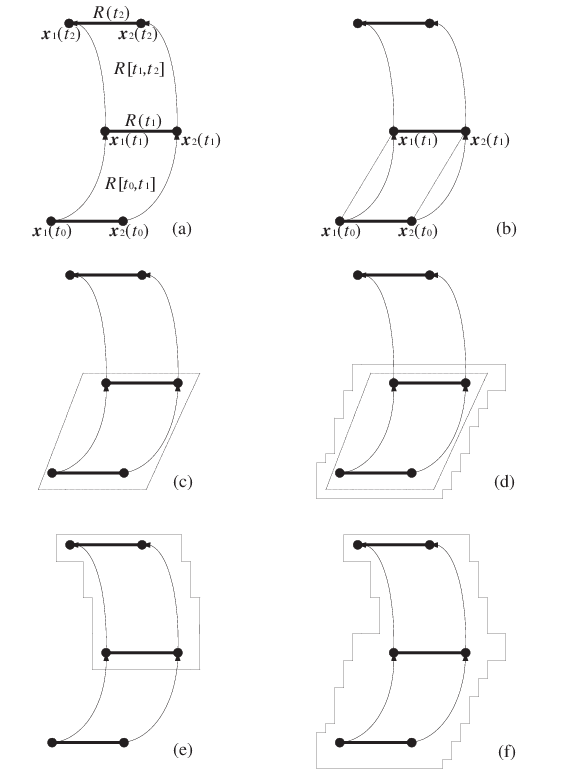
\includegraphics{ddt.png}
\caption{Reach set approximation by union of rectangles}\label{chap_intro:ddtfig}\end{figure}

The algorithm works as follows. First, given the set of initial
conditions defined as a polytope, the evolution in time of the
polytope’s extreme points is computed (\hyperref[chap_intro:ddtfig]{figure  \ref*{chap_intro:ddtfig}} (a)).

$R(t_1)$ in \hyperref[chap_intro:ddtfig]{figure  \ref*{chap_intro:ddtfig}} (a) is the reach set of the system at
time $t_1$, and $R[t_0, t_1]$ is the set of all points that
can be reached during $[t_0, t_1]$. Second, the algorithm computes
the convex hull of vertices of both, the initial polytope and
$R(t_1)$ (\hyperref[chap_intro:ddtfig]{figure  \ref*{chap_intro:ddtfig}} (b)). The resulting polytope is then
bloated to include all the reachable states in $[t_0,t_1]$ (\hyperref[chap_intro:ddtfig]{figure  \ref*{chap_intro:ddtfig}} (c)).
Finally, this overapproximating polytope is in its turn
overapproximated by the union of rectangles (\hyperref[chap_intro:ddtfig]{figure  \ref*{chap_intro:ddtfig}} (d)). The
same procedure is repeated for the next time interval $[t_1,t_2]$,
and the union of both rectangular approximations is taken (\hyperref[chap_intro:ddtfig]{figure  \ref*{chap_intro:ddtfig}} (e,f)),
and so on. Rectangular polytopes are easy to represent
and the number of facets grows linearly with dimension, but a large
number of rectangles must be used to assure the approximation is not
overly conservative. Besides, the important part of this method is again
the convex hull calculation whose implementation relies on the same
CDD/CDD+ library. This limits the dimension of the system and time
interval for which it is feasible to calculate the reach set.

Polytopes can give arbitrarily close approximations to any convex set,
but the number of vertices can grow prohibitively large and, as shown in
Avis, Bremner, and Seidel (1997), the computation of a polytope by its
convex hull becomes intractable for large number of vertices in high
dimensions.

The method of zonotopes for approximation of reach sets Girard (2005;
A.Girard, Guernic, and O.Maler 2006; “MATISSE Homepage”) uses a special
class of polytopes (see (“Zonotope Methods on Wolfgang Kühn Homepage”))
of the form,
\begin{gather}
\begin{split}Z=\{x \in {\bf R}^n ~|~
x=c+\sum_{i=1}^p\alpha_ig_i,~ -1\leqslant\alpha_i\leqslant1\},\end{split}\notag
\end{gather}
wherein $c$ and $g_1, ..., g_p$ are vectors in
${\bf R}^n$. Thus, a zonotope $Z$ is represented by its
center $c$ and ‘generator’ vectors $g_1, ..., g_p$. The
value $p/n$ is called the order of the zonotope. The main benefit
of zonotopes over general polytopes is that a symmetric polytope can be
represented more compactly than a general polytope. The geometric sum of
two zonotopes is a zonotope:
\begin{gather}
\begin{split}Z(c_1, G_1)\oplus Z(c_2, G_2) = Z(c_1+c_2, [G_1 ~ G_2]),\end{split}\notag\\\begin{split}\end{split}\notag
\end{gather}
wherein $G_1$ and $G_2$ are matrices whose columns are
generator vectors, and $[G_1 ~ G_2]$ is their concatenation. Thus,
in the reach set computation, the order of the zonotope increases by
$p/n$ with every time step. This difficulty can be averted by
limiting the number of generator vectors, and overapproximating
zonotopes whose number of generator vectors exceeds the limit by lower
order zonotopes. The benefits of the compact zonotype representation,
however, appear to diminish because in order to plot them or check if
they intersect with given objects and compute those intersections, these
operations are performed after converting zonotopes to polytopes.

CheckMate (“CheckMate Homepage”) is a Matlab toolbox that can evaluate
specifications for trajectories starting from the set of initial
(continuous) states corresponding to the parameter values at the
vertices of the parameter set. This provides preliminary insight into
whether the specifications will be true for all parameter values. The
method of oriented rectangluar polytopes for external approximation of
reach sets is introduced in Stursberg and Krogh (2003). The basic idea
is to construct an oriented rectangular hull of the reach set for every
time step, whose orientation is determined by the singular value
decomposition of the sample covariance matrix for the states reachable
from the vertices of the initial polytope. The limitation of CheckMate
and the method of oriented rectangles is that only autonomous (i.e.
uncontrolled) systems, or systems with fixed input are allowed, and only
an external approximation of the reach set is provided.

All the methods described so far employ the notion of time step, and
calculate the reach set or its approximation at each time step. This
approach can be used only with discrete-time systems. By contrast, the
analytic methods which we are about to discuss, provide a formula or
differential equation describing the (continuous) time evolution of the
reach set or its approximation.

The level set method Mitchell and Tomlin (2000; “Level Set Toolbox
Homepage”) deals with general nonlinear controlled systems and gives
exact representation of their reach sets, but requires solving the HJB
equation and finding the set of states that belong to sub-zero level set
of the value function. The method (“Level Set Toolbox Homepage”) is
impractical for systems of dimension higher than three.

Requiem (“Requiem Homepage”) is a Mathematica notebook which, given a
linear system, the set of initial conditions and control bounds,
symbolically computes the exact reach set, using the experimental
quantifier elimination package. Quantifier elimination is the removal of
all quantifiers (the universal quantifier $\forall$ and the
existential quantifier $\exists$) from a quantified system. Each
quantified formula is substituted with quantifier-free expression with
operations $+$, $\times$, $=$ and $<$. For
example, consider the discrete-time system
\begin{gather}
\begin{split}x_{k+1} = Ax_k + Bu_k\end{split}\notag\\\begin{split}\end{split}\notag
\end{gather}
with $A=\left[\begin{array}{cc}0 & 1\\0 & 0\end{array}\right]$
and $B=\left[\begin{array}{c}0\\1\end{array}\right]$.

For initial conditions $x_0\in\{x\in {\bf R}^2 ~|~ \|x\|_{\infty} \leqslant1\}$ and
controls $u_k\in\{u\in {\bf R} ~|~ -1\leqslant u\leqslant1\}$, the
reach set for $k\geqslant0$ is given by the quantified formula
\begin{gather}
\begin{split}\{ x\in{\bf R}^2 ~|~ \exists x_0, ~~ \exists k\geqslant0, ~~
\exists u_i, ~ 0\leqslant i\leqslant k: ~~
x = A^kx_0+\sum_{i=0}^{k-1}A^{k-i-1}Bu_i \},\end{split}\notag
\end{gather}
which is equivalent to the quantifier-free expression
\begin{gather}
\begin{split}-1\leqslant[1 ~~ 0]x\leqslant1 ~ \wedge ~ -1\leqslant[0 ~~ 1]x\leqslant1.\end{split}\notag\\\begin{split}\end{split}\notag
\end{gather}
It is proved in Lafferriere, Pappas, and Yovine (2001) that for
continuous-time systems, $\dot{x}(t) = Ax(t) + Bu(t)$, if
$A$ is constant and nilpotent or is diagonalizable with rational
real or purely imaginary eigenvalues, and with suitable restrictions on
the control and initial conditions, the quantifier elimination package
returns a quantifier free formula describing the reach set. Quantifier
elimination has limited applicability.

The reach set approximation via parallelotopes Kostousova (2001) employs
the idea of parametrization described in Kurzhanski and Varaiya (2000)
for ellipsoids. The reach set is represented as the intersection of
tight external, and the union of tight internal, parallelotopes. The
evolution equations for the centers and orientation matrices of both
external and internal parallelotopes are provided. This method also
finds controls that can drive the system to the boundary points of the
reach set, similarly to Varaiya (1998) and Kurzhanski and Varaiya
(2000). It works for general linear systems. The computation to solve
the evolution equation for tight approximating parallelotopes, however,
is more involved than that for ellipsoids, and for discrete-time systems
this method does not deal with singular state transition matrices.

\emph{Ellipsoidal Toolbox} (ET) implements in MATLAB the ellipsoidal calculus
Kurzhanski and Vályi (1997) and its application to the reachability
analysis of continuous-time Kurzhanski and Varaiya (2000), discrete-time
A. A. Kurzhanskiy (2007), possibly time-varying linear systems, and
linear systems with disturbances A.B.Kurzhanski and P.Varaiya (2001),
for which ET calculates both open-loop and close-loop reach sets. The
ellipsoidal calculus provides the following benefits:
\begin{itemize}
\item {} 
The complexity of the ellipsoidal representation is quadratic in the
dimension of the state space, and linear in the number of time steps.

\item {} 
It is possible to exactly represent the reach set of linear system
through both external and internal ellipsoids.

\item {} 
It is possible to single out individual external and internal
approximating ellipsoids that are optimal to some given criterion
(e.g. trace, volume, diameter), or combination of such criteria.

\item {} 
We obtain simple analytical expressions for the control that steers
the state to a desired target.

\end{itemize}

The report is organized as follows. Chapter 2 describes the operations
of the ellipsoidal calculus: affine transformation, geometric sum,
geometric difference, intersections with hyperplane, ellipsoid,
halfspace and polytope, calculation of maximum ellipsoid, calculation of
minimum ellipsoid. Chapter 3 presents the reachability problem and
ellipsoidal methods for the reach set approximation. Chapter 4 contains
\emph{Ellipsoidal Toolbox} installation and quick start instructions, and
lists the software packages used by the toolbox. Chapter 5 describes
structures and objects implemented and used in toolbox. Also it
describes the implementation of methods from chapters 2 and 3 and
visualization routines. Chapter 6 describes structures and objects
implemented and used in the toolbox. Chapter 6 gives examples of how to
use the toolbox. Chapter 7 collects some conclusions and plans for
future toolbox development. The functions provided by the toolbox
together with their descriptions are listed in appendix A.


\chapter{Ellipsoidal Calculus}
\label{chap_ellcalc:ellipsoidal-calculus}\label{chap_ellcalc::doc}

\section{Basic Notions}
\label{chap_ellcalc:basic-notions}
We start with basic definitions.
Ellipsoid ${\mathcal E}(q,Q)$ in
${\bf R}^n$ with center $q$ and shape matrix $Q$ is
the set
\phantomsection\label{chap_ellcalc:equation-ellipsoid}\begin{gather}
\begin{split}{\mathcal E}(q,Q) = \{ x \in {\bf R}^n ~|~ \langle (x-q), Q^{-1}(x-q)\rangle\leqslant1 \},\end{split}\label{chap_ellcalc-ellipsoid}
\end{gather}
wherein $Q$ is positive definite ($Q=Q^T$ and
$\langle x, Qx\rangle>0$ for all nonzero $x\in{\bf R}^n$).
Here $\langle\cdot,\cdot\rangle$ denotes inner
product. The support function of a set
${\mathcal X}\subseteq{\bf R}^n$ is
\begin{gather}
\begin{split}\rho(l~|~{\mathcal X}) = \sup_{x\in{\mathcal X}} \langle l,x\rangle.\end{split}\notag\\\begin{split}\end{split}\notag
\end{gather}
In particular, the support function of the ellipsoid \eqref{chap_ellcalc-ellipsoid} is
\phantomsection\label{chap_ellcalc:equation-ellsupp}\begin{gather}
\begin{split}\rho(l~|~{\mathcal E}(q,Q)) = \langle l, q\rangle + \langle l, Ql\rangle^{1/2}.\end{split}\label{chap_ellcalc-ellsupp}
\end{gather}
Although in \eqref{chap_ellcalc-ellipsoid} $Q$ is assumed to be positive definite,
in practice we may deal with situations when $Q$ is singular, that
is, with degenerate ellipsoids flat in those directions for which the
corresponding eigenvalues are zero. Therefore, it is useful to give an
alternative definition of an ellipsoid using the expression \eqref{chap_ellcalc-ellsupp}.
Ellipsoid ${\mathcal E}(q,Q)$ in ${\bf R}^n$ with center
$q$ and shape matrix $Q$ is the set
\phantomsection\label{chap_ellcalc:equation-ellipsoid2}\begin{gather}
\begin{split}{\mathcal E}(q,Q) = \{ x \in {\bf R}^n ~|~
\langle l,x\rangle\leqslant\langle l,q\rangle + \langle l,Ql\rangle^{1/2}
\mbox{ for all } l\in{\bf R}^n \},\end{split}\label{chap_ellcalc-ellipsoid2}
\end{gather}
wherein matrix $Q$ is positive semidefinite ($Q=Q^T$ and
$\langle x, Qx\rangle\geqslant0$ for all $x\in{\bf R}^n$).
The volume of ellipsoid ${\mathcal E}(q,Q)$ is
\phantomsection\label{chap_ellcalc:equation-ellvolume}\begin{gather}
\begin{split}{\bf Vol}(E(q,Q)) = {\bf Vol}_{\langle x,x\rangle\leqslant1}\sqrt{\det Q},\end{split}\label{chap_ellcalc-ellvolume}
\end{gather}
where ${\bf Vol}_{\langle x,x\rangle\leqslant1}$ is the volume of
the unit ball in ${\bf R}^n$:
\phantomsection\label{chap_ellcalc:equation-ellunitball}\begin{gather}
\begin{split}{\bf Vol}_{\langle x,x\rangle\leqslant1} = \left\{\begin{array}{ll}
\frac{\pi^{n/2}}{(n/2)!}, &
\mbox{ for even } n,\\
\frac{2^n\pi^{(n-1)/2}\left((n-1)/2\right)!}{n!}, &
\mbox{ for odd } n. \end{array}\right.\end{split}\label{chap_ellcalc-ellunitball}
\end{gather}
The distance from ${\mathcal E}(q,Q)$ to the fixed point $a$
is
\phantomsection\label{chap_ellcalc:equation-dist_point}\begin{gather}
\begin{split}{\bf dist}({\mathcal E}(q,Q),a) = \max_{\langle l,l\rangle=1}\left(\langle l,a\rangle -
\rho(l ~|~ {\mathcal E}(q,Q)) \right) =
\max_{\langle l,l\rangle=1}\left(\langle l,a\rangle - \langle l,q\rangle -
\langle l,Ql\rangle^{1/2}\right).\end{split}\label{chap_ellcalc-dist_point}
\end{gather}
If ${\bf dist}({\mathcal E}(q,Q),a) > 0$, $a$ lies outside
${\mathcal E}(q,Q)$; if
${\bf dist}({\mathcal E}(q,Q),a) = 0$, $a$ is a boundary
point of ${\mathcal E}(q,Q)$; if
${\bf dist}({\mathcal E}(q,Q),a) < 0$, $a$ is an internal
point of ${\mathcal E}(q,Q)$.

Given two ellipsoids, ${\mathcal E}(q_1,Q_1)$ and
${\mathcal E}(q_2,Q_2)$, the distance between them is
\phantomsection\label{chap_ellcalc:equation-dist_ell}\begin{gather}
\begin{split}\begin{aligned}
{\bf dist}({\mathcal E}(q_1,Q_1),{\mathcal E}(q_2,Q_2)) & = & \max_{\langle l,l\rangle=1}
\left(-\rho(-l ~|~ {\mathcal E}(q_1,Q_1)) - \rho(l ~|~ {\mathcal E}(q_2,Q_2))\right) \\
& = & \max_{\langle l,l\rangle=1}\left(\langle l,q_1\rangle -
\langle l,Q_1l\rangle^{1/2} - \langle l,q_2\rangle -
\langle l,Q_2l\rangle^{1/2}\right).
\end{aligned}\end{split}\label{chap_ellcalc-dist_ell}
\end{gather}
If ${\bf dist}({\mathcal E}(q_1,Q_1),{\mathcal E}(q_2,Q_2)) > 0$,
the ellipsoids have no common points; if
${\bf dist}({\mathcal E}(q_1,Q_1),{\mathcal E}(q_2,Q_2)) = 0$, the
ellipsoids have one common point - they touch; if
${\bf dist}({\mathcal E}(q_1,Q_1),{\mathcal E}(q_2,Q_2)) < 0$, the
ellipsoids intersect.

Finding ${\bf dist}({\mathcal E}(q_1,Q_1),{\mathcal E}(q_2,Q_2))$
using QCQP is
\begin{gather}
\begin{split}d({\mathcal E}(q_1,Q_1),{\mathcal E}(q_2,Q_2)) = \min \langle (x-y), (x-y)\rangle\end{split}\notag\\\begin{split}\end{split}\notag
\end{gather}
subject to:
\begin{gather}
\begin{split}\begin{aligned}
\langle (q_1-x), Q_1^{-1}(q_1-x)\rangle & \leqslant& 1,\\
\langle (q_2-x), Q_2^{-1}(q_2-y)\rangle & \leqslant& 1,\end{aligned}\end{split}\notag
\end{gather}
where
\begin{gather}
\begin{split}d({\mathcal E}(q_1,Q_1),{\mathcal E}(q_2,Q_2))=\left\{\begin{array}{ll}
{\bf dist}^2({\mathcal E}(q_1,Q_1),{\mathcal E}(q_2,Q_2)) &
\mbox{ if } {\bf dist}({\mathcal E}(q_1,Q_1),{\mathcal E}(q_2,Q_2))>0, \\
0 & \mbox{ otherwise}. \end{array}\right.\end{split}\notag
\end{gather}
Checking if $k$ nondegenerate ellipsoids
${\mathcal E}(q_1,Q_1),\cdots,{\mathcal E}(q_k,Q_k)$ have nonempty
intersection, can be cast as a quadratically constrained quadratic
programming (QCQP) problem:
\begin{gather}
\begin{split}\min 0\end{split}\notag\\\begin{split}\end{split}\notag
\end{gather}
subject to:
\begin{gather}
\begin{split}\langle (x-q_i),Q_i^{-1}(x-q_i)\rangle - 1 \leqslant0, ~~~ i=1,\cdots,k.\end{split}\notag\\\begin{split}\end{split}\notag
\end{gather}
If this problem is feasible, the intersection is nonempty. Given
compact convex set ${\mathcal X}\subseteq{\bf R}^n$, its polar
set, denoted ${\mathcal X}^\circ$, is
\begin{gather}
\begin{split}{\mathcal X}^\circ = \{x\in{\bf R}^n ~|~ \langle x,y\rangle\leqslant1, ~ y\in{\mathcal X}\},\end{split}\notag\\\begin{split}\end{split}\notag
\end{gather}
or, equivalently,
\begin{gather}
\begin{split}{\mathcal X}^\circ = \{l\in{\bf R}^n ~|~ \rho(l ~|~ {\mathcal X})\leqslant1\}.\end{split}\notag\\\begin{split}\end{split}\notag
\end{gather}
The properties of the polar set are
\begin{itemize}
\item {} 
If ${\mathcal X}$ contains the origin,
$({\mathcal X}^\circ)^\circ = {\mathcal X}$;

\item {} 
If ${\mathcal X}_1\subseteq{\mathcal X}_2$,
${\mathcal X}_2^\circ\subseteq{\mathcal X}_1^\circ$;

\item {} 
For any nonsingular matrix $A\in{\bf R}^{n\times n}$,
$(A{\mathcal X})^\circ = (A^T)^{-1}{\mathcal X}^\circ$.

\end{itemize}

If a nondegenerate ellipsoid ${\mathcal E}(q,Q)$ contains the
origin, its polar set is also an ellipsoid:
\begin{gather}
\begin{split}\begin{aligned}
{\mathcal E}^\circ(q,Q) & = & \{l\in{\bf R}^n ~|~ \langle l,q\rangle +
\langle l,Ql\rangle^{1/2}\leqslant1 \}\\
& = & \{l\in{\bf R}^n ~|~ \langle l,(Q-qq^T)^{-1}l\rangle +
2\langle l,q\rangle\leqslant1 \}\\
& = & \{l\in{\bf R}^n ~|~ \langle(l+(Q-qq^T)^{-1}q),
(Q-qq^T)(l+(Q-qq^T)^{-1}q)\rangle\leqslant1+\langle q,(Q-qq^T)^{-1}q\rangle \}.\end{aligned}\end{split}\notag
\end{gather}
The special case is
\begin{gather}
\begin{split}{\mathcal E}^\circ(0,Q) = {\mathcal E}(0,Q^{-1}).\end{split}\notag\\\begin{split}\end{split}\notag
\end{gather}
Given $k$ compact sets
${\mathcal X}_1, \cdots, {\mathcal X}_k\subseteq{\bf R}^n$, their
geometric (Minkowski) sum is
\phantomsection\label{chap_ellcalc:equation-minksum}\begin{gather}
\begin{split}{\mathcal X}_1\oplus\cdots\oplus{\mathcal X}_k=\bigcup_{x_1\in{\mathcal X}_1}\cdots\bigcup_{x_k\in{\mathcal X}_k}
\{x_1 + \cdots + x_k\} .\end{split}\label{chap_ellcalc-minksum}
\end{gather}
Given two compact sets
${\mathcal X}_1, {\mathcal X}_2 \subseteq{\bf R}^n$, their
geometric (Minkowski) difference is
\phantomsection\label{chap_ellcalc:equation-minkdiff}\begin{gather}
\begin{split}{\mathcal X}_1\dot{-}{\mathcal X}_2 = \{x\in{\bf R}^n ~|~ x + {\mathcal X}_2 \subseteq {\mathcal X}_1 \}.\end{split}\label{chap_ellcalc-minkdiff}
\end{gather}
Ellipsoidal calculus concerns the following set of operations:
\begin{itemize}
\item {} 
affine transformation of ellipsoid;

\item {} 
geometric sum of finite number of ellipsoids;

\item {} 
geometric difference of two ellipsoids;

\item {} 
intersection of finite number of ellipsoids.

\end{itemize}

These operations occur in reachability calculation and verification of
piecewise affine dynamical systems. The result of all of these
operations, except for the affine transformation, is \emph{not} generally an
ellipsoid but some convex set, for which we can compute external and
internal ellipsoidal approximations.

Additional operations implemented in the \emph{Ellipsoidal Toolbox} include
external and internal approximations of intersections of ellipsoids with
hyperplanes, halfspaces and polytopes. Hyperplane $H(c,\gamma)$ in
${\bf R}^n$ is the set
\phantomsection\label{chap_ellcalc:equation-hyperplane}\begin{gather}
\begin{split}H = \{x\in{\bf R}^n ~|~ \langle c, x\rangle = \gamma\}\end{split}\label{chap_ellcalc-hyperplane}
\end{gather}
with $c\in{\bf R}^n$ and $\gamma\in{\bf R}$ fixed.
The distance from ellipsoid ${\mathcal E}(q,Q)$ to
hyperplane $H(c,\gamma)$ is
\phantomsection\label{chap_ellcalc:equation-dist_hp}\begin{gather}
\begin{split}{\bf dist}({\mathcal E}(q,Q),H(c,\gamma)) =
\frac{\left|\gamma-\langle c,q\rangle\right| -
\langle c,Qc\rangle^{1/2}}{\langle c,c\rangle^{1/2}}.\end{split}\label{chap_ellcalc-dist_hp}
\end{gather}
If ${\bf dist}({\mathcal E}(q,Q),H(c,\gamma))>0$, the ellipsoid
and the hyperplane do not intersect; if
${\bf dist}({\mathcal E}(q,Q),H(c,\gamma))=0$, the hyperplane is a
supporting hyperplane for the ellipsoid; if
${\bf dist}({\mathcal E}(q,Q),H(c,\gamma))<0$, the ellipsoid
intersects the hyperplane. The intersection of an ellipsoid with a
hyperplane is always an ellipsoid and can be computed directly.

Checking if the intersection of $k$ nondegenerate ellipsoids
$E(q_1,Q_1),\cdots,{\mathcal E}(q_k,Q_k)$ intersects hyperplane
$H(c,\gamma)$, is equivalent to the feasibility check of the QCQP
problem:
\begin{gather}
\begin{split}\min 0\end{split}\notag\\\begin{split}\end{split}\notag
\end{gather}
subject to:
\begin{gather}
\begin{split}\begin{aligned}
\langle (x-q_i),Q_i^{-1}(x-q_i)\rangle - 1 \leqslant0, & & i=1,\cdots,k,\\
\langle c, x\rangle - \gamma = 0. & &\end{aligned}\end{split}\notag
\end{gather}
A hyperplane defines two (closed) \emph{halfspaces}:
\phantomsection\label{chap_ellcalc:equation-halfspace1}\begin{gather}
\begin{split}{\bf S}_1 = \{x\in{\bf R}^n ~|~ \langle c, x\rangle \leqslant\gamma\}\end{split}\label{chap_ellcalc-halfspace1}
\end{gather}
and
\phantomsection\label{chap_ellcalc:equation-halfspace2}\begin{gather}
\begin{split}{\bf S}_2 = \{x\in{\bf R}^n ~|~ \langle c, x\rangle \geqslant\gamma\}.\end{split}\label{chap_ellcalc-halfspace2}
\end{gather}
To avoid confusion, however, we shall further assume that a hyperplane
$H(c,\gamma)$ specifies the halfspace in the sense \eqref{chap_ellcalc-halfspace1}.
In order to refer to the other halfspace, the same hyperplane should be
defined as $H(-c,-\gamma)$.

The idea behind the calculation of intersection of an ellipsoid with a
halfspace is to treat the halfspace as an unbounded ellipsoid, that is,
as the ellipsoid with the shape matrix all but one of whose eigenvalues
are $\infty$.
Polytope $P(C,g)$ is the
intersection of a finite number of closed halfspaces:
\phantomsection\label{chap_ellcalc:equation-polytope}\begin{gather}
\begin{split}P = \{x\in{\bf R}^n ~|~ Cx\leqslant g\},\end{split}\label{chap_ellcalc-polytope}
\end{gather}
wherein $C=[c_1 ~ \cdots ~ c_m]^T\in{\bf R}^{m\times n}$ and
$g=[\gamma_1 ~ \cdots ~ \gamma_m]^T\in{\bf R}^m$.
The distance
from ellipsoid ${\mathcal E}(q,Q)$ to the polytope $P(C,g)$
is
\phantomsection\label{chap_ellcalc:equation-dist_poly}\begin{gather}
\begin{split}{\bf dist}({\mathcal E}(q,Q),P(C,g))=\min_{y\in P(C,g)}{\bf dist}({\mathcal E}(q,Q),y),\end{split}\label{chap_ellcalc-dist_poly}
\end{gather}
where ${\bf dist}({\mathcal E}(q,Q),y)$ comes from
({[}dist:sub:\emph{p}oint{]}). If
${\bf dist}({\mathcal E}(q,Q),P(C,g))>0$, the ellipsoid and the
polytope do not intersect; if
${\bf dist}({\mathcal E}(q,Q),P(C,g))=0$, the ellipsoid touches
the polytope; if ${\bf dist}({\mathcal E}(q,Q),P(C,g))<0$, the
ellipsoid intersects the polytope.

Checking if the intersection of $k$ nondegenerate ellipsoids
$E(q_1,Q_1),\cdots,{\mathcal E}(q_k,Q_k)$ intersects polytope
$P(C,g)$ is equivalent to the feasibility check of the QCQP
problem:
\begin{gather}
\begin{split}\min 0\end{split}\notag\\\begin{split}\end{split}\notag
\end{gather}
subject to:
\begin{gather}
\begin{split}\begin{aligned}
\langle (x-q_i),Q_i^{-1}(x-q_i)\rangle - 1 \leqslant0, & & i=1,\cdots,k,\\
\langle c_j, x\rangle - \gamma_j \leqslant0, & & j=1,\cdots,m.\end{aligned}\end{split}\notag
\end{gather}

\section{Operations with Ellipsoids}
\label{chap_ellcalc:operations-with-ellipsoids}

\subsection{Affine Transformation}
\label{chap_ellcalc:affine-transformation}
The simplest operation with ellipsoids is an affine transformation. Let
ellipsoid ${\mathcal E}(q,Q)\subseteq{\bf R}^n$, matrix
$A\in{\bf R}^{m\times n}$ and vector $b\in{\bf R}^m$. Then
\phantomsection\label{chap_ellcalc:equation-affinetrans}\begin{gather}
\begin{split}A{\mathcal E}(q,Q) + b = {\mathcal E}(Aq+b, AQA^T) .\end{split}\label{chap_ellcalc-affinetrans}
\end{gather}
Thus, ellipsoids are preserved under affine transformation. If the rows
of $A$ are linearly independent (which implies
$m\leqslant n$), and $b=0$, the affine transformation is
called \emph{projection}.


\subsection{Geometric Sum}
\label{chap_ellcalc:geometric-sum}
Consider the geometric sum \eqref{chap_ellcalc-minksum} in which
${\mathcal X}_1,\cdots$,${\mathcal X}_k$ are nondegenerate
ellipsoids ${\mathcal E}(q_1,Q_1),\cdots$,
${\mathcal E}(q_k,Q_k)\subseteq{\bf R}^n$. The resulting set is
not generally an ellipsoid. However, it can be tightly approximated by
the parametrized families of external and internal ellipsoids.

Let parameter $l$ be some nonzero vector in ${\bf R}^n$.
Then the external approximation ${\mathcal E}(q,Q_l^+)$ and the
internal approximation ${\mathcal E}(q,Q_l^-)$ of the sum
${\mathcal E}(q_1,Q_1)\oplus\cdots\oplus{\mathcal E}(q_k,Q_k)$ are
\emph{tight} along direction $l$, i.e.,
\begin{gather}
\begin{split}{\mathcal E}(q,Q_l^-)\subseteq{\mathcal E}(q_1,Q_1)\oplus\cdots\oplus{\mathcal E}(q_k,Q_k)
\subseteq{\mathcal E}(q,Q_l^+)\end{split}\notag
\end{gather}
and
\begin{gather}
\begin{split}\rho(\pm l ~|~ {\mathcal E}(q,Q_l^-)) =
\rho(\pm l ~|~ {\mathcal E}(q_1,Q_1)\oplus\cdots\oplus{\mathcal E}(q_k,Q_k)) =
\rho(\pm l ~|~ {\mathcal E}(q,Q_l^+)).\end{split}\notag
\end{gather}
Here the center $q$ is
\phantomsection\label{chap_ellcalc:equation-minksum_c}\begin{gather}
\begin{split}q = q_1 + \cdots + q_k ,\end{split}\label{chap_ellcalc-minksum_c}
\end{gather}
the shape matrix of the external ellipsoid $Q_l^+$ is
\phantomsection\label{chap_ellcalc:equation-minksum_ea}\begin{gather}
\begin{split}Q_l^+ = \left(\langle l,Q_1l\rangle^{1/2} + \cdots
+ \langle l,Q_kl\rangle^{1/2}\right)
\left(\frac{1}{\langle l,Q_1l\rangle^{1/2}}Q_1 + \cdots +
\frac{1}{\langle l,Q_kl\rangle^{1/2}}Q_k\right),\end{split}\label{chap_ellcalc-minksum_ea}
\end{gather}
and the shape matrix of the internal ellipsoid $Q_l^-$ is
\phantomsection\label{chap_ellcalc:equation-minksum_ia}\begin{gather}
\begin{split}Q_l^- = \left(Q_1^{1/2} + S_2Q_2^{1/2} + \cdots + S_kQ_k^{1/2}\right)^T
\left(Q_1^{1/2} + S_2Q_2^{1/2} + \cdots + S_kQ_k^{1/2}\right),\end{split}\label{chap_ellcalc-minksum_ia}
\end{gather}
with matrices $S_i$, $i=2,\cdots,k$, being orthogonal
($S_iS_i^T=I$) and such that vectors
$Q_1^{1/2}l, S_2Q_2^{1/2}l, \cdots, S_kQ_k^{1/2}l$ are parallel.

Varying vector $l$ we get exact external and internal
approximations,
\begin{gather}
\begin{split}\bigcup_{\langle l,l\rangle=1} {\mathcal E}(q,Q_l^-) =
{\mathcal E}(q_1,Q_1)\oplus\cdots\oplus{\mathcal E}(q_k,Q_k) =
\bigcap_{\langle l,l\rangle=1} {\mathcal E}(q,Q_l^+) .\end{split}\notag
\end{gather}
For proofs of formulas given in this section, see Kurzhanski and Vályi
(1997), Kurzhanski and Varaiya (2000).

One last comment is about how to find orthogonal matrices
$S_2,\cdots,S_k$ that align vectors
$Q_2^{1/2}l, \cdots, Q_k^{1/2}l$ with $Q_1^{1/2}l$. Let
$v_1$ and $v_2$ be some unit vectors in ${\bf R}^n$.
We have to find matrix $S$ such that
$Sv_2\uparrow\uparrow v_1$. We suggest explicit formulas for the
calculation of this matrix ( Dariyn and Kurzhanski (2012)):
\phantomsection\label{chap_ellcalc:equation-valign1}\begin{gather}
\begin{split}&&T = I + Q_1(S - I)Q_1^T, \\\end{split}\label{chap_ellcalc-valign1}
\end{gather}\phantomsection\label{chap_ellcalc:equation-valign2}\begin{gather}
\begin{split}&&S = \begin{pmatrix}
     c & s\\
     -s & c
    \end{pmatrix},\quad c = \langle\hat{v_1},\ \hat{v_2}\rangle,\ \quad s = \sqrt{1 - c^2},\ \quad \hat{v_i} = \dfrac{v_i}{\|v_i\|}\\\end{split}\label{chap_ellcalc-valign2}
\end{gather}\phantomsection\label{chap_ellcalc:equation-valign3}\begin{gather}
\begin{split}&&Q_1 = [q_1 \, q_2]\in \mathbb{R}^{n\times2},\ \quad q_1 = \hat{v_1},\ \quad q_2 = \begin{cases}
s^{-1}(\hat{v_2} - c\hat{v_1}),& s\ne 0\\
0,& s = 0.
\end{cases}\end{split}\label{chap_ellcalc-valign3}
\end{gather}

\subsection{Geometric Difference}
\label{chap_ellcalc:geometric-difference}
Consider the geometric difference \eqref{chap_ellcalc-minkdiff} in which the sets
${\mathcal X}_1$ and ${\mathcal X}_2$ are nondegenerate
ellipsoids ${\mathcal E}(q_1,Q_1)$ and
${\mathcal E}(q_2,Q_2)$. We say that ellipsoid
${\mathcal E}(q_1,Q_1)$ is \emph{bigger} than ellipsoid
${\mathcal E}(q_2,Q_2)$ if
\begin{gather}
\begin{split}{\mathcal E}(0,Q_2) \subseteq {\mathcal E}(0,Q_1).\end{split}\notag\\\begin{split}\end{split}\notag
\end{gather}
If this condition is not fulfilled, the geometric difference
${\mathcal E}(q_1,Q_1)\dot{-}{\mathcal E}(q_2,Q_2)$ is an empty
set:
\begin{gather}
\begin{split}{\mathcal E}(0,Q_2) \not\subseteq {\mathcal E}(0,Q_1) ~~~ \Rightarrow ~~~
{\mathcal E}(q_1,Q_1) \dot{-}{\mathcal E}(q_2,Q_2) = \emptyset.\end{split}\notag
\end{gather}
If ${\mathcal E}(q_1,Q_1)$ is bigger than
${\mathcal E}(q_2,Q_2)$ and ${\mathcal E}(q_2,Q_2)$ is
bigger than ${\mathcal E}(q_1,Q_1)$, in other words, if
$Q_1=Q_2$,
\begin{gather}
\begin{split}{\mathcal E}(q_1,Q_1) \dot{-}{\mathcal E}(q_2,Q_2) = \{q_1-q_2\} ~~~ \mbox{and} ~~~
{\mathcal E}(q_2,Q_2) \dot{-}{\mathcal E}(q_1,Q_1) = \{q_2-q_1\}.\end{split}\notag
\end{gather}
To check if ellipsoid ${\mathcal E}(q_1,Q_1)$ is bigger than
ellipsoid ${\mathcal E}(q_2,Q_2)$, we perform simultaneous
diagonalization of matrices $Q_1$ and $Q_2$, that is, we
find matrix $T$ such that
\begin{gather}
\begin{split}TQ_1T^T = I ~~~ \mbox{and} ~~~ TQ_2T^T=D,\end{split}\notag\\\begin{split}\end{split}\notag
\end{gather}
where $D$ is some diagonal matrix. Simultaneous diagonalization
of $Q_1$ and $Q_2$ is possible because both are symmetric
positive definite (see Gantmacher (1960)). To find such matrix
$T$, we first do the SVD of $Q_1$:
\phantomsection\label{chap_ellcalc:equation-simdiag1}\begin{gather}
\begin{split}Q_1 = U_1\Sigma_1V_1^T .\end{split}\label{chap_ellcalc-simdiag1}
\end{gather}
Then the SVD of matrix
$\Sigma_1^{-1/2}U_1^TQ_2U_1\Sigma_1^{-1/2}$:
\phantomsection\label{chap_ellcalc:equation-simdiag2}\begin{gather}
\begin{split}\Sigma_1^{-1/2}U_1^TQ_2U_1\Sigma_1^{-1/2} = U_2\Sigma_2V_2^T.\end{split}\label{chap_ellcalc-simdiag2}
\end{gather}
Now, $T$ is defined as
\phantomsection\label{chap_ellcalc:equation-simdiag3}\begin{gather}
\begin{split}T = U_2^T \Sigma_1^{-1/2}U_1^T.\end{split}\label{chap_ellcalc-simdiag3}
\end{gather}
If the biggest diagonal element (eigenvalue) of matrix $D=TQ_2T^T$
is less than or equal to $1$,
${\mathcal E}(0,Q_2)\subseteq{\mathcal E}(0,Q_1)$.

Once it is established that ellipsoid ${\mathcal E}(q_1,Q_1)$ is
bigger than ellipsoid ${\mathcal E}(q_2,Q_2)$, we know that their
geometric difference
${\mathcal E}(q_1,Q_1)\dot{-}{\mathcal E}(q_2,Q_2)$ is a nonempty
convex compact set. Although it is not generally an ellipsoid, we can
find tight external and internal approximations of this set parametrized
by vector $l\in{\bf R}^n$. Unlike geometric sum, however,
ellipsoidal approximations for the geometric difference do not exist for
every direction $l$. Vectors for which the approximations do not
exist are called \emph{bad directions}.

Given two ellipsoids ${\mathcal E}(q_1,Q_1)$ and
${\mathcal E}(q_2,Q_2)$ with
${\mathcal E}(0,Q_2)\subseteq{\mathcal E}(0,Q_1)$, $l$ is a
bad direction if
\begin{gather}
\begin{split}\frac{\langle l,Q_1l\rangle^{1/2}}{\langle l,Q_2l\rangle^{1/2}}>r,\end{split}\notag\\\begin{split}\end{split}\notag
\end{gather}
in which $r$ is a minimal root of the equation
\begin{gather}
\begin{split}{\bf det}(Q_1-rQ_2) = 0.\end{split}\notag\\\begin{split}\end{split}\notag
\end{gather}
To find $r$, compute matrix $T$ by \eqref{chap_ellcalc-simdiag1}-\eqref{chap_ellcalc-simdiag3}
and define
\begin{gather}
\begin{split}r = \frac{1}{\max({\bf diag}(TQ_2T^T))}.\end{split}\notag\\\begin{split}\end{split}\notag
\end{gather}
If $l$ is \emph{not} a bad direction, we can find tight external and
internal ellipsoidal approximations ${\mathcal E}(q,Q^+_l)$ and
${\mathcal E}(q,Q^-_l)$ such that
\begin{gather}
\begin{split}{\mathcal E}(q,Q^-_l)\subseteq{\mathcal E}(q_1,Q_1)\dot{-}{\mathcal E}(q_2,Q_2)\subseteq{\mathcal E}(q,Q^+_l)\end{split}\notag\\\begin{split}\end{split}\notag
\end{gather}
and
\begin{gather}
\begin{split}\rho(\pm l ~|~ {\mathcal E}(q,Q_l^-)) =
\rho(\pm l ~|~ {\mathcal E}(q_1,Q_1)\dot{-}{\mathcal E}(q_2,Q_2)) =
\rho(\pm l ~|~ {\mathcal E}(q,Q_l^+)).\end{split}\notag
\end{gather}
The center $q$ is
\phantomsection\label{chap_ellcalc:equation-minkdiff_c}\begin{gather}
\begin{split}q = q_1 - q_2;\end{split}\label{chap_ellcalc-minkdiff_c}
\end{gather}
the shape matrix of the internal ellipsoid $Q^-_l$ is
\begin{gather}
\begin{split}\begin{aligned}
&& P = \frac{\sqrt{\langle l, Q_1 l\rangle}}{\sqrt{\langle l, Q_2 \rangle}};\nonumber\\
&& Q^-_l = \left(1 - \dfrac{1}{P}\right)Q_1 + \left(1 - P\right)Q_2.
\label{minkdiff_ia}\end{aligned}\end{split}\notag
\end{gather}
and the shape matrix of the external ellipsoid $Q^+_l$ is
\phantomsection\label{chap_ellcalc:equation-minkdiff_ea}\begin{gather}
\begin{split}Q^+_l = \left(Q_1^{1/2} - SQ_2^{1/2}\right)^T
\left(Q_1^{1/2} - SQ_2^{1/2}\right).\end{split}\label{chap_ellcalc-minkdiff_ea}
\end{gather}
Here $S$ is an orthogonal matrix such that vectors
$Q_1^{1/2}l$ and $SQ_2^{1/2}l$ are parallel. $S$ is
found from \eqref{chap_ellcalc-valign1}-\eqref{chap_ellcalc-valign3}, with $v_1=Q_2^{1/2}l$ and
$v_2=Q_1^{1/2}l$.

Running $l$ over all unit directions that are not bad, we get
\begin{gather}
\begin{split}\bigcup_{\langle l,l\rangle=1} {\mathcal E}(q,Q_l^-) =
{\mathcal E}(q_1,Q_1)\dot{-}{\mathcal E}(q_2,Q_2) =
\bigcap_{\langle l,l\rangle=1} {\mathcal E}(q,Q_l^+) .\end{split}\notag
\end{gather}
For proofs of formulas given in this section, see Kurzhanski and Vályi
(1997).


\subsection{Geometric Difference-Sum}
\label{chap_ellcalc:geometric-difference-sum}
Given ellipsoids ${\mathcal E}(q_1,Q_1)$,
${\mathcal E}(q_2,Q_2)$ and ${\mathcal E}(q_3,Q_3)$, it is
possible to compute families of external and internal approximating
ellipsoids for
\phantomsection\label{chap_ellcalc:equation-minkmp}\begin{gather}
\begin{split}{\mathcal E}(q_1,Q_1) \dot{-} {\mathcal E}(q_2,Q_2) \oplus {\mathcal E}(q_3,Q_3)\end{split}\label{chap_ellcalc-minkmp}
\end{gather}
parametrized by direction $l$, if this set is nonempty
(${\mathcal E}(0,Q_2)\subseteq{\mathcal E}(0,Q_1)$).

First, using the result of the previous section, for any direction
$l$ that is not bad, we obtain tight external
${\mathcal E}(q_1-q_2, Q_l^{0+})$ and internal
${\mathcal E}(q_1-q_2, Q_l^{0-})$ approximations of the set
${\mathcal E}(q_1,Q_1)\dot{-}{\mathcal E}(q_2,Q_2)$.

The second and last step is, using the result of section 2.2.2, to find
tight external ellipsoidal approximation
${\mathcal E}(q_1-q_2+q_3,Q_l^+)$ of the sum
${\mathcal E}(q_1-q_2,Q_l^{0+})\oplus{\mathcal E}(q_3,Q_3)$, and
tight internal ellipsoidal approximation
${\mathcal E}(q_1-q_2+q_3,Q_l^-)$ for the sum
${\mathcal E}(q_1-q_2,Q_l^{0-})\oplus{\mathcal E}(q_3,Q_3)$.

As a result, we get
\begin{gather}
\begin{split}{\mathcal E}(q_1-q_2+q_3,Q_l^-) \subseteq
{\mathcal E}(q_1,Q_1)\dot{-}{\mathcal E}(q_2,Q_2)\oplus{\mathcal E}(q_3,Q_3) \subseteq
{\mathcal E}(q_1-q_2+q_3,Q_l^+)\end{split}\notag
\end{gather}
and
\begin{gather}
\begin{split}\rho(\pm l ~|~{\mathcal E}(q_1-q_2+q_3,Q_l^-)) =
\rho(\pm l ~|~ {\mathcal E}(q_1,Q_1)\dot{-}{\mathcal E}(q_2,Q_2)\oplus{\mathcal E}(q_3,Q_3)) =
\rho(\pm l ~|~ {\mathcal E}(q_1-q_2+q_3,Q_l^+)).\end{split}\notag
\end{gather}
Running $l$ over all unit vectors that are not bad, this
translates to
\begin{gather}
\begin{split}\bigcup_{\langle l,l\rangle=1} {\mathcal E}(q_1-q_2+q_3,Q_l^-) =
{\mathcal E}(q_1,Q_1)\dot{-}{\mathcal E}(q_2,Q_2)\oplus{\mathcal E}(q_3,Q_3) =
\bigcap_{\langle l,l\rangle=1} {\mathcal E}(q_1-q_2+q_3,Q_l^+) .\end{split}\notag
\end{gather}

\subsection{Geometric Sum-Difference}
\label{chap_ellcalc:geometric-sum-difference}
Given ellipsoids ${\mathcal E}(q_1,Q1)$,
${\mathcal E}(q_2,Q_2)$ and ${\mathcal E}(q_3,Q_3)$, it is
possible to compute families of external and internal approximating
ellipsoids for
\phantomsection\label{chap_ellcalc:equation-minkpm}\begin{gather}
\begin{split}{\mathcal E}(q_1,Q_1) \oplus {\mathcal E}(q_2,Q_2) \dot{-} {\mathcal E}(q_3,Q_3)\end{split}\label{chap_ellcalc-minkpm}
\end{gather}
parametrized by direction $l$, if this set is nonempty
(${\mathcal E}(0,Q_3)\subseteq{\mathcal E}(0,Q_1)\oplus{\mathcal E}(0,Q_2)$).

First, using the result of section 2.2.2, we obtain tight external
${\mathcal E}(q_1+q_2,Q_l^{0+})$ and internal
${\mathcal E}(q_1+q_2,Q_l^{0-})$ ellipsoidal approximations of the
set ${\mathcal E}(q_1,Q_1)\oplus{\mathcal E}(q_2,Q_2)$. In order
for the set \eqref{chap_ellcalc-minkpm} to be nonempty, inclusion
${\mathcal E}(0,Q_3)\subseteq{\mathcal E}(0,Q_l^{0+})$ must be
true for any $l$. Note, however, that even if \eqref{chap_ellcalc-minkpm} is
nonempty, it may be that
${\mathcal E}(0,Q_3)\not\subseteq{\mathcal E}(0,Q_l^{0-})$, then
internal approximation for this direction does not exist.

Assuming that \eqref{chap_ellcalc-minkpm} is nonempty and
${\mathcal E}(0,Q_3)\subseteq{\mathcal E}(0,Q_l^{0-})$, the second
step would be, using the results of section 2.2.3, to compute tight
external ellipsoidal approximation
${\mathcal E}(q_1+q_2-q_3,Q_l^+)$ of the difference
${\mathcal E}(q_1+q_2,Q_l^{0+})\dot{-}{\mathcal E}(q_3,Q_3)$,
which exists only if $l$ is not bad, and tight internal
ellipsoidal approximation ${\mathcal E}(q_1+q_2-q_3,Q_l^-)$ of the
difference
${\mathcal E}(q_1+q_2,Q_l^{0-})\dot{-}{\mathcal E}(q_3,Q_3)$,
which exists only if $l$ is not bad for this difference.

If approximation ${\mathcal E}(q_1+q_2-q_3,Q_l^+)$ exists, then
\begin{gather}
\begin{split}{\mathcal E}(q_1,Q_1)\oplus{\mathcal E}(q_2,Q_2)\dot{-}{\mathcal E}(q_3,Q_3) \subseteq
{\mathcal E}(q_1+q_2-q_3,Q_l^+)\end{split}\notag
\end{gather}
and
\begin{gather}
\begin{split}\rho(\pm l ~|~ {\mathcal E}(q_1,Q_1)\oplus{\mathcal E}(q_2,Q_2)\dot{-}{\mathcal E}(q_3,Q_3)) =
\rho(\pm l ~|~ {\mathcal E}(q_1+q_2-q_3,Q_l^+)).\end{split}\notag
\end{gather}
If approximation ${\mathcal E}(q_1+q_2-q_3,Q_l^-)$ exists, then
\begin{gather}
\begin{split}{\mathcal E}(q_1+q_2-q_3,Q_l^-) \subseteq
{\mathcal E}(q_1,Q_1)\oplus{\mathcal E}(q_2,Q_2)\dot{-}{\mathcal E}(q_3,Q_3)\end{split}\notag
\end{gather}
and
\begin{gather}
\begin{split}\rho(\pm l ~|~{\mathcal E}(q_1+q_2-q_3,Q_l^-)) =
\rho(\pm l ~|~ {\mathcal E}(q_1,Q_1)\oplus{\mathcal E}(q_2,Q_2)\dot{-}{\mathcal E}(q_3,Q_3)) .\end{split}\notag
\end{gather}
For any fixed direction $l$ it may be the case that neither
external nor internal tight ellipsoidal approximations exist.


\subsection{Intersection of Ellipsoid and Hyperplane}
\label{chap_ellcalc:intersection-of-ellipsoid-and-hyperplane}
Let nondegenerate ellipsoid ${\mathcal E}(q,Q)$ and hyperplane
$H(c,\gamma)$ be such that
${\bf dist}({\mathcal E}(q,Q),H(c,\gamma))<0$. In other words,
\begin{gather}
\begin{split}{\mathcal E}_H(w,W) = {\mathcal E}(q,Q)\cap H(c,\gamma) \neq \emptyset .\end{split}\notag\\\begin{split}\end{split}\notag
\end{gather}
The intersection of ellipsoid with hyperplane, if nonempty, is always
an ellipsoid. Here we show how to find it.

First of all, we transform the hyperplane $H(c,\gamma)$ into
$H([1~0~\cdots~0]^T, 0)$ by the affine transformation
\begin{gather}
\begin{split}y = Sx - \frac{\gamma}{\langle c,c\rangle^{1/2}}Sc,\end{split}\notag\\\begin{split}\end{split}\notag
\end{gather}
where $S$ is an orthogonal matrix found by \eqref{chap_ellcalc-valign1}-\eqref{chap_ellcalc-valign3}
with $v_1=c$ and $v_2=[1~0~\cdots~0]^T$. The ellipsoid in
the new coordinates becomes ${\mathcal E}(q',Q')$ with
\begin{gather}
\begin{split}\begin{aligned}
q' & = & q-\frac{\gamma}{\langle c,c\rangle^{1/2}}Sc, \\
Q' & = & SQS^T.\end{aligned}\end{split}\notag
\end{gather}
Define matrix $M=Q'^{-1}$; $m_{11}$ is its element in
position $(1,1)$, $\bar{m}$ is the first column of $M$
without the first element, and $\bar{M}$ is the submatrix of
$M$ obtained by stripping $M$ of its first row and first
column:
\begin{gather}
\begin{split}M = \left[\begin{array}{c|cl}
m_{11} & & \bar{m}^T\\
 & \\
\hline
 & \\
\bar{m} & & \bar{M}\end{array}\right].\end{split}\notag
\end{gather}
The ellipsoid resulting from the intersection is
${\mathcal E}_H(w',W')$ with
\begin{gather}
\begin{split}\begin{aligned}
w' & = & q' + q_1'\left[\begin{array}{c}
-1\\
\bar{M}^{-1}\bar{m}\end{array}\right],\\
W' & = & \left(1-q_1'^2(m_{11}-
\langle\bar{m},\bar{M}^{-1}\bar{m}\rangle)\right)\left[\begin{array}{c|cl}
0 & & {\bf 0}\\
 & \\
\hline
 & \\
{\bf 0} & & \bar{M}^{-1}\end{array}\right],\end{aligned}\end{split}\notag
\end{gather}
in which $q_1'$ represents the first element of vector $q'$.

Finally, it remains to do the inverse transform of the coordinates to
obtain ellipsoid ${\mathcal E}_H(w,W)$:
\begin{gather}
\begin{split}\begin{aligned}
w & = & S^Tw' + \frac{\gamma}{\langle c,c\rangle^{1/2}}c, \\
W & = & S^TW'S.\end{aligned}\end{split}\notag
\end{gather}

\subsection{Intersection of Ellipsoid and Ellipsoid}
\label{chap_ellcalc:intersection-of-ellipsoid-and-ellipsoid}
Given two nondegenerate ellipsoids ${\mathcal E}(q_1,Q_1)$ and
${\mathcal E}(q_2,Q_2)$,
${\bf dist}({\mathcal E}(q_1,Q_1),{\mathcal E}(q_2,Q_2))<0$
implies that
\begin{gather}
\begin{split}{\mathcal E}(q_1,Q_1)\cap{\mathcal E}(q_2,Q_2)\neq\emptyset .\end{split}\notag\\\begin{split}\end{split}\notag
\end{gather}
This intersection can be approximated by ellipsoids from the outside
and from the inside. Trivially, both ${\mathcal E}(q_1,Q_1)$ and
${\mathcal E}(q_2,Q_2)$ are external approximations of this
intersection. Here, however, we show how to find the external
ellipsoidal approximation of minimal volume.

Define matrices
\begin{gather}
\begin{split}W_1 = Q_1^{-1}, ~~~~ W_2 = Q_2^{-1} .\label{wmatrices}\end{split}\notag\\\begin{split}\end{split}\notag
\end{gather}
Minimal volume external ellipsoidal approximation
${\mathcal E}(q+,Q^+)$ of the intersection
${\mathcal E}(q_1,Q_1)\cap{\mathcal E}(q_2,Q_2)$ is determined
from the set of equations:
\phantomsection\label{chap_ellcalc:equation-fusion1}\begin{gather}
\begin{split}Q^+  = \alpha X^{-1}, \\\end{split}\label{chap_ellcalc-fusion1}
\end{gather}\phantomsection\label{chap_ellcalc:equation-fusion2}\begin{gather}
\begin{split}X  =  \pi W_1 + (1-\pi)W_2,\\\end{split}\label{chap_ellcalc-fusion2}
\end{gather}\phantomsection\label{chap_ellcalc:equation-fusion3}\begin{gather}
\begin{split}\alpha  =  1-\pi(1-\pi)\langle(q_2-q_1), W_2X^{-1}W_1(q_2-q_1)\rangle, \\\end{split}\label{chap_ellcalc-fusion3}
\end{gather}\phantomsection\label{chap_ellcalc:equation-fusion4}\begin{gather}
\begin{split}q^+  = X^{-1}(\pi W_1q_1 + (1-\pi)W_2q_2), \\\end{split}\label{chap_ellcalc-fusion4}
\end{gather}\phantomsection\label{chap_ellcalc:equation-fusion5}\begin{gather}
\begin{split}0 &=  \alpha({\bf det}(X))^2{\bf trace}(X^{-1}(W_1-W_2)) - {}\\
  &- n({\bf det}(X))^2 (2\langle q^+,W_1q_1-W_2q_2\rangle + \langle q^+,(W_2-W_1)q^+\rangle - {}\\
  &- \langle q_1,W_1q_1\rangle + \langle q_2,W_2q_2\rangle),\end{split}\label{chap_ellcalc-fusion5}
\end{gather}
with $0\leqslant\pi\leqslant1$. We substitute $X$,
$\alpha$, $q^+$ defined in \eqref{chap_ellcalc-fusion2}-\eqref{chap_ellcalc-fusion4} into
\eqref{chap_ellcalc-fusion5} and get a polynomial of degree $2n-1$ with respect to
$\pi$, which has only one root in the interval $[0,1]$,
$\pi_0$. Then, substituting $\pi=\pi_0$ into
\eqref{chap_ellcalc-fusion1}-\eqref{chap_ellcalc-fusion4}, we obtain $q^+$ and $Q^+$. Special
cases are $\pi_0=1$, whence
${\mathcal E}(q^+,Q^+)={\mathcal E}(q_1,Q_1)$, and
$\pi_0=0$, whence
${\mathcal E}(q^+,Q^+)={\mathcal E}(q_2,Q_2)$. These situations
may occur if, for example, one ellipsoid is contained in the other:
\begin{gather}
\begin{split}{\mathcal E}(q_1,Q_1)\subseteq{\mathcal E}(q_2,Q_2) & \Rightarrow & \pi_0 = 1,\\\end{split}\notag\\\begin{split}{\mathcal E}(q_2,Q_2)\subseteq{\mathcal E}(q_1,Q_1) & \Rightarrow & \pi_0 = 0.\\\end{split}\notag
\end{gather}
The proof that the system of equations \eqref{chap_ellcalc-fusion1}-\eqref{chap_ellcalc-fusion5} correctly
defines the minimal volume external ellipsoidal approximationi of the
intersection ${\mathcal E}(q_1,Q_1)\cap{\mathcal E}(q_2,Q_2)$ is
given in L. Ros (2002).

To find the internal approximating ellipsoid
${\mathcal E}(q^-,Q^-)\subseteq{\mathcal E}(q_1,Q_1)\cap{\mathcal E}(q_2,Q_2)$,
define
\phantomsection\label{chap_ellcalc:equation-beta1}\begin{gather}
\begin{split}\beta_1 & = & \min_{\langle x,W_2x\rangle=1}\langle x,W_1x\rangle,\\\end{split}\label{chap_ellcalc-beta1}
\end{gather}\phantomsection\label{chap_ellcalc:equation-beta2}\begin{gather}
\begin{split}\beta_2 & = & \min_{\langle x,W_1x\rangle=1}\langle x,W_2x\rangle,\end{split}\label{chap_ellcalc-beta2}
\end{gather}
Notice that \eqref{chap_ellcalc-beta1} and \eqref{chap_ellcalc-beta2} are QCQP problems. Parameters
$\beta_1$ and $\beta_2$ are invariant with respect to affine
coordinate transformation and describe the position of ellipsoids
${\mathcal E}(q_1,Q_1)$, ${\mathcal E}(q_2,Q_2)$ with
respect to each other:
\begin{gather}
\begin{split}\beta_1\geqslant1,~\beta_2\geqslant1 & \Rightarrow &
{\bf int}({\mathcal E}(q_1,Q_1)\cap{\mathcal E}(q_2,Q_2))=\emptyset, \\\end{split}\notag\\\begin{split}\beta_1\geqslant1,~\beta_2\leqslant1 & \Rightarrow & {\mathcal E}(q_1,Q_1)\subseteq{\mathcal E}(q_2,Q_2), \\\end{split}\notag\\\begin{split}\beta_1\leqslant1,~\beta_2\geqslant1 & \Rightarrow & {\mathcal E}(q_2,Q_2)\subseteq{\mathcal E}(q_1,Q_1), \\\end{split}\notag\\\begin{split}\beta_1<1,~\beta_2<1 & \Rightarrow &
{\bf int}({\mathcal E}(q_1,Q_1)\cap{\mathcal E}(q_2,Q_2))\neq\emptyset \\\end{split}\notag\\\begin{split}& & \mbox{and} ~ {\mathcal E}(q_1,Q_1)\not\subseteq{\mathcal E}(q_2,Q_2) \\\end{split}\notag\\\begin{split}& & \mbox{and} ~ {\mathcal E}(q_2,Q_2)\not\subseteq{\mathcal E}(q_1,Q_1).\end{split}\notag
\end{gather}
Define parametrized family of internal ellipsoids
${\mathcal E}(q^-_{\theta_1\theta_2},Q^-_{\theta_1\theta_2})$ with
\phantomsection\label{chap_ellcalc:equation-paramell1}\begin{gather}
\begin{split}q^-_{\theta_1\theta_2}  =  (\theta_1W_1 +
\theta_2W_2)^{-1}(\theta_1W_1q_1 + \theta_2W_2q_2),\\\end{split}\label{chap_ellcalc-paramell1}
\end{gather}\phantomsection\label{chap_ellcalc:equation-paramell2}\begin{gather}
\begin{split}Q^-_{\theta_1\theta_2} =  (1 - \theta_1\langle q_1,W_1q_1\rangle -
\theta_2\langle q_2,W_2q_2\rangle +
\langle q^-_{\theta_1\theta_2},(Q^-)^{-1}q^-_{\theta_1\theta_2}\rangle)
(\theta_1W_1 + \theta_2W_2)^{-1} .\end{split}\label{chap_ellcalc-paramell2}
\end{gather}
The best internal ellipsoid
${\mathcal E}(q^-_{\hat{\theta}_1\hat{\theta}_2},Q^-_{\hat{\theta}_1\hat{\theta}_2})$
in the class \eqref{chap_ellcalc-paramell1}-\eqref{chap_ellcalc-paramell2}, namely, such that
\begin{gather}
\begin{split}{\mathcal E}(q^-_{{\theta}_1{\theta}_2},Q^-_{{\theta}_1{\theta}_2})\subseteq
{\mathcal E}(q^-_{\hat{\theta}_1\hat{\theta}_2},Q^-_{\hat{\theta}_1\hat{\theta}_2})
\subseteq {\mathcal E}(q_1,Q_1)\cap{\mathcal E}(q_2,Q_2)\end{split}\notag
\end{gather}
for all $0\leqslant\theta_1,\theta_2\leqslant1$, is specified by
the parameters
\phantomsection\label{chap_ellcalc:equation-thetapar}\begin{gather}
\begin{split}\hat{\theta}_1 = \frac{1-\hat{\beta}_2}{1-\hat{\beta}_1\hat{\beta}_2}, ~~~~
\hat{\theta}_2 = \frac{1-\hat{\beta}_1}{1-\hat{\beta}_1\hat{\beta}_2},\end{split}\label{chap_ellcalc-thetapar}
\end{gather}
with
\begin{gather}
\begin{split}\hat{\beta}_1=\min(1,\beta_1), ~~~~ \hat{\beta}_2=\min(1,\beta_2).\end{split}\notag\\\begin{split}\end{split}\notag
\end{gather}
It is the ellipsoid that we look for:
${\mathcal E}(q^-,Q^-)={\mathcal E}(q^-_{\hat{\theta}_1\hat{\theta}_2},Q^-_{\hat{\theta}_1\hat{\theta}_2})$.
Two special cases are
\begin{gather}
\begin{split}\hat{\theta}_1=1, ~ \hat{\theta}_2=0 ~~~ \Rightarrow ~~~
{\mathcal E}(q_1,Q_1)\subseteq{\mathcal E}(q_2,Q_2) ~~~ \Rightarrow ~~~
{\mathcal E}(q^-,Q^-)={\mathcal E}(q_1,Q_1),\end{split}\notag
\end{gather}
and
\begin{gather}
\begin{split}\hat{\theta}_1=0, ~ \hat{\theta}_2=1 ~~~ \Rightarrow ~~~
{\mathcal E}(q_2,Q_2)\subseteq{\mathcal E}(q_1,Q_1) ~~~ \Rightarrow ~~~
{\mathcal E}(q^-,Q^-)={\mathcal E}(q_2,Q_2).\end{split}\notag
\end{gather}
The method of finding the internal ellipsoidal approximation of the
intersection of two ellipsoids is described in Vazhentsev (1999).


\subsection{Intersection of Ellipsoid and Halfspace}
\label{chap_ellcalc:intersection-of-ellipsoid-and-halfspace}
Finding the intersection of ellipsoid and halfspace can be reduced to
finding the intersection of two ellipsoids, one of which is unbounded.
Let ${\mathcal E}(q_1,Q_1)$ be a nondegenerate ellipsoid and let
$H(c,\gamma)$ define the halfspace
\begin{gather}
\begin{split}{\bf S}(c,\gamma) = \{x\in{\bf R}^n ~|~ \langle c,x\rangle\leqslant\gamma\}.\end{split}\notag\\\begin{split}\end{split}\notag
\end{gather}
We have to determine if the intersection
${\mathcal E}(q_1,Q_1)\cap{\bf S}(c,\gamma)$ is empty, and if not,
find its external and internal ellipsoidal approximations,
${\mathcal E}(q^+,Q^+)$ and ${\mathcal E}(q^-,Q^-)$. Two
trivial situations are:
\begin{itemize}
\item {} 
${\bf dist}({\mathcal E}(q_1,Q_1),H(c,\gamma))>0$ and
$\langle c, q_1\rangle>0$, which implies that
${\mathcal E}(q_1,Q_1)\cap{\bf S}(c,\gamma)=\emptyset$;

\item {} 
${\bf dist}({\mathcal E}(q_1,Q_1),H(c,\gamma))>0$ and
$\langle c, q_1\rangle<0$, so that
${\mathcal E}(q_1,Q_1)\subseteq{\bf S}(c,\gamma)$, and then
${\mathcal E}(q^+,Q^+)={\mathcal E}(q^-,Q^-)={\mathcal E}(q_1,Q_1)$.

\end{itemize}

In case ${\bf dist}({\mathcal E}(q_1,Q_1),H(c,\gamma)<0$, i.e. the
ellipsoid intersects the hyperplane,
\begin{gather}
\begin{split}{\mathcal E}(q_1,Q_1)\cap{\bf S}(c,\gamma) =
{\mathcal E}(q_1,Q_1)\cap\{x ~|~ \langle (x-q_2),W_2(x-q_2)\rangle\leqslant1\},\end{split}\notag
\end{gather}
with
\phantomsection\label{chap_ellcalc:equation-hsell1}\begin{gather}
\begin{split}q_2  =  (\gamma + 2\sqrt{\overline{\lambda}})c,\\\end{split}\label{chap_ellcalc-hsell1}
\end{gather}\phantomsection\label{chap_ellcalc:equation-hsell2}\begin{gather}
\begin{split}W_2  =  \frac{1}{4\overline{\lambda}}cc^T,\end{split}\label{chap_ellcalc-hsell2}
\end{gather}
$\overline{\lambda}$ being the biggest eigenvalue of matrix
$Q_1$. After defining $W_1=Q_1^{-1}$, we obtain
${\mathcal E}(q^+,Q^+)$ from equations \eqref{chap_ellcalc-fusion1}-\eqref{chap_ellcalc-fusion5}, and
${\mathcal E}(q^-,Q^-)$ from \eqref{chap_ellcalc-paramell1}-\eqref{chap_ellcalc-paramell2},
\eqref{chap_ellcalc-thetapar}.

\textbf{Remark.} Notice that matrix $W_2$ has rank $1$, which
makes it singular for $n>1$. Nevertheless, expressions
\eqref{chap_ellcalc-fusion1}-\eqref{chap_ellcalc-fusion2}, \eqref{chap_ellcalc-paramell1}-\eqref{chap_ellcalc-paramell2} make sense because
$W_1$ is nonsingular, $\pi_0\neq0$ and
$\hat{\theta}_1\neq0$.

To find the ellipsoidal approximations ${\mathcal E}(q^+,Q^+)$ and
${\mathcal E}(q^-,Q^-)$ of the intersection of ellipsoid
${\mathcal E}(q,Q)$ and polytope $P(C,g)$,
$C\in{\bf R}^{m\times n}$, $b\in{\bf R}^m$, such that
\begin{gather}
\begin{split}{\mathcal E}(q^-,Q^-)\subseteq{\mathcal E}(q,Q)\cap P(C,g)\subseteq{\mathcal E}(q^+,Q^+),\end{split}\notag\\\begin{split}\end{split}\notag
\end{gather}
we first compute
\begin{gather}
\begin{split}{\mathcal E}(q^-_1,Q^-_1)\subseteq{\mathcal E}(q,Q)\cap{\bf S}(c_1,\gamma_1)\subseteq
{\mathcal E}(q^+_1,Q^+_1),\end{split}\notag
\end{gather}
wherein ${\bf S}(c_1,\gamma_1)$ is the halfspace defined by the
first row of matrix $C$, $c_1$, and the first element of
vector $g$, $\gamma_1$. Then, one by one, we get
\begin{gather}
\begin{split}\begin{aligned}
& & {\mathcal E}(q^-_2,Q^-_2)\subseteq{\mathcal E}(q^-_1,Q^-_1)\cap{\bf S}(c_2,\gamma_2), ~~~
{\mathcal E}(q^+_1,Q^+_1)\cap{\bf S}(c_2,\gamma_2)\subseteq{\mathcal E}(q^+_2,Q^+_2), \\
& & {\mathcal E}(q^-_3,Q^-_3)\subseteq{\mathcal E}(q^-_2,Q^-_2)\cap{\bf S}(c_3,\gamma_3), ~~~
{\mathcal E}(q^+_2,Q^+_2)\cap{\bf S}(c_3,\gamma_3)\subseteq{\mathcal E}(q^+_3,Q^+_3), \\
& & \cdots \\
& & {\mathcal E}(q^-_m,Q^-_m)\subseteq{\mathcal E}(q^-_{m-1},Q^-_{m-1})\cap{\bf S}(c_m,\gamma_m), ~~~
{\mathcal E}(q^+_{m-1},Q^+_{m-1})\cap{\bf S}(c_m,\gamma_m)\subseteq{\mathcal E}(q^+_m,Q^+_m), \\\end{aligned}\end{split}\notag
\end{gather}
The resulting ellipsoidal approximations are
\begin{gather}
\begin{split}{\mathcal E}(q^+,Q^+)={\mathcal E}(q^+_m,Q^+_m), ~~~~ {\mathcal E}(q^-,Q^-)={\mathcal E}(q^-_m,Q^-_m) .\end{split}\notag\\\begin{split}\end{split}\notag
\end{gather}

\subsection{Checking if $\EE(q_1,Q_1)\subseteq\EE(q_2,Q_2)$}
\label{chap_ellcalc:checking-if}
Theorem of alternatives, also known as $S$-procedure Boyd and
Vandenberghe (2004), states that the implication
\begin{gather}
\begin{split}\langle x, A_1x\rangle + 2\langle b_1,x\rangle + c_1 \leqslant0
~~ \Rightarrow ~~
\langle x, A_2x\rangle + 2\langle b_2,x\rangle + c_2 \leqslant0,\end{split}\notag
\end{gather}
where $A_i\in{\bf R}^{n\times n}$ are symmetric matrices,
$b_i\in{\bf R}^n$, $c_i\in{\bf R}$, $i=1,2$, holds if
and only if there exists $\lambda>0$ such that
\begin{gather}
\begin{split}\left[\begin{array}{cc}
A_2 & b_2\\
b_2^T & c_2\end{array}\right]
\preceq
\lambda\left[\begin{array}{cc}
A_1 & b_1\\
b_1^T & c_1\end{array}\right].\end{split}\notag
\end{gather}
By $S$-procedure,
${\mathcal E}(q_1,Q_1)\subseteq{\mathcal E}(q_2,Q_2)$ (both
ellipsoids are assumed to be nondegenerate) if and only if the following
SDP problem is feasible:
\begin{gather}
\begin{split}\min 0\end{split}\notag\\\begin{split}\end{split}\notag
\end{gather}
subject to:
\begin{gather}
\begin{split}\begin{aligned}
\lambda & > & 0, \\
\left[\begin{array}{cc}
Q_2^{-1} & -Q_2^{-1}q_2\\
(-Q_2^{-1}q_2)^T & q_2^TQ_2^{-1}q_2-1\end{array}\right]
& \preceq &
\lambda \left[\begin{array}{cc}
Q_1^{-1} & -Q_1^{-1}q_1\\
(-Q_1^{-1}q_1)^T & q_1^TQ_1^{-1}q_1-1\end{array}\right]\end{aligned}\end{split}\notag
\end{gather}
where $\lambda\in{\bf R}$ is the variable.


\subsection{Minimum Volume Ellipsoids}
\label{chap_ellcalc:minimum-volume-ellipsoids}
The minimum volume ellipsoid that contains set $S$ is called
\emph{Löwner-John ellipsoid} of the set $S$. To characterize it we
rewrite general ellipsoid ${\mathcal E}(q,Q)$ as
\begin{gather}
\begin{split}{\mathcal E}(q,Q) = \{x ~|~ \langle (Ax + b), (Ax + b)\rangle \},\end{split}\notag\\\begin{split}\end{split}\notag
\end{gather}
where
\begin{gather}
\begin{split}A = Q^{-1/2} ~~~ \mbox{ and } ~~~ b = -Aq .\end{split}\notag\\\begin{split}\end{split}\notag
\end{gather}
For positive definite matrix $A$, the volume of
${\mathcal E}(q,Q)$ is proportional to $\det A^{-1}$. So,
finding the minimum volume ellipsoid containing $S$ can be
expressed as semidefinite programming (SDP) problem
\begin{gather}
\begin{split}\min \log \det A^{-1}\end{split}\notag\\\begin{split}\end{split}\notag
\end{gather}
subject to:
\begin{gather}
\begin{split}\sup_{v\in S} \langle (Av + b), (Av + b)\rangle \leqslant1,\end{split}\notag\\\begin{split}\end{split}\notag
\end{gather}
where the variables are $A\in{\bf R}^{n\times n}$ and
$b\in{\bf R}^n$, and there is an implicit constraint
$A\succ 0$ ($A$ is positive definite). The objective and
constraint functions are both convex in $A$ and $b$, so this
problem is convex. Evaluating the constraint function, however, requires
solving a convex maximization problem, and is tractable only in certain
special cases.

For a finite set $S=\{x_1,\cdots,x_m\}\subset{\bf R}^n$, an
ellipsoid covers $S$ if and only if it covers its convex hull. So,
finding the minimum volume ellipsoid covering $S$ is the same as
finding the minimum volume ellipsoid containing the polytope
${\bf conv}\{x_1,\cdots,x_m\}$. The SDP problem is
\begin{gather}
\begin{split}\min \log \det A^{-1}\end{split}\notag\\\begin{split}\end{split}\notag
\end{gather}
subject to:
\begin{gather}
\begin{split}\begin{aligned}
A & \succ & 0, \\
\langle (Ax_i + b), (Ax_i + b)\rangle & \leqslant& 1, ~~~ i=1..m.\end{aligned}\end{split}\notag
\end{gather}
We can find the minimum volume ellipsoid containing the union of
ellipsoids $\bigcup_{i=1}^m{\mathcal E}(q_i,Q_i)$. Using the fact
that for $i=1..m$
${\mathcal E}(q_i,Q_i)\subseteq{\mathcal E}(q,Q)$ if and only if
there exists $\lambda_i>0$ such that
\begin{gather}
\begin{split}\left[\begin{array}{cc}
A^2 - \lambda_i Q_i^{-1} & Ab + \lambda_i Q_i^{-1}q_i\\
(Ab + \lambda_i Q_i^{-1}q_i)^T & b^Tb-1 - \lambda_i (q_i^TQ_i^{-1}q_i-1) \end{array}
\right] \preceq 0 .\end{split}\notag
\end{gather}
Changing variable $\tilde{b}=Ab$, we get convex SDP in the
variables $A$, $\tilde{b}$, and
$\lambda_1,\cdots,\lambda_m$:
\begin{gather}
\begin{split}\min \log \det A^{-1}\end{split}\notag\\\begin{split}\end{split}\notag
\end{gather}
subject to:
\begin{gather}
\begin{split}\begin{aligned}
\lambda_i & > & 0,\\
\left[\begin{array}{ccc}
A^2-\lambda_iQ_i^{-1} & \tilde{b}+\lambda_iQ_i^{-1}q_i & 0 \\
(\tilde{b}+\lambda_iQ_i^{-1}q_i)^T & -1-\lambda_i(q_i^TQ_i^{-1}q_i-1) & \tilde{b}^T \\
0 & \tilde{b} & -A^2\end{array}\right] & \preceq & 0, ~~~ i=1..m.\end{aligned}\end{split}\notag
\end{gather}
After $A$ and $b$ are found,
\begin{gather}
\begin{split}q=-A^{-1}b ~~~ \mbox{ and } ~~~ Q=(A^TA)^{-1}.\end{split}\notag\\\begin{split}\end{split}\notag
\end{gather}
The results on the minimum volume ellipsoids are explained and proven in
Boyd and Vandenberghe (2004).


\subsection{Maximum Volume Ellipsoids}
\label{chap_ellcalc:maximum-volume-ellipsoids}
Consider a problem of finding the maximum volume ellipsoid that lies
inside a bounded convex set $S$ with nonempty interior. To
formulate this problem we rewrite general ellipsoid
${\mathcal E}(q,Q)$ as
\begin{gather}
\begin{split}{\mathcal E}(q,Q) = \{Bx + q ~|~ \langle x,x\rangle\leqslant1\},\end{split}\notag\\\begin{split}\end{split}\notag
\end{gather}
where $B=Q^{1/2}$, so the volume of ${\mathcal E}(q,Q)$ is
proportional to $\det B$.

The maximum volume ellipsoid that lies inside $S$ can be found by
solving the following SDP problem:
\begin{gather}
\begin{split}\max \log \det B\end{split}\notag\\\begin{split}\end{split}\notag
\end{gather}
subject to:
\begin{gather}
\begin{split}\sup_{\langle v,v\rangle\leqslant1} I_S(Bv+q)\leqslant0 ,\end{split}\notag\\\begin{split}\end{split}\notag
\end{gather}
in the variables $B\in{\bf R}^{n\times n}$ - symmetric matrix,
and $q\in{\bf R}^n$, with implicit constraint $B\succ 0$,
where $I_S$ is the indicator function:
\begin{gather}
\begin{split}I_S(x) = \left\{\begin{array}{ll}
0, & \mbox{ if } x\in S,\\
\infty, & \mbox{ otherwise.}\end{array}\right.\end{split}\notag
\end{gather}
In case of polytope, $S=P(C,g)$ with $P(C,g)$ defined in
\eqref{chap_ellcalc-polytope}, the SDP has the form
\begin{gather}
\begin{split}\min \log \det B^{-1}\end{split}\notag\\\begin{split}\end{split}\notag
\end{gather}
subject to:
\begin{gather}
\begin{split}\begin{aligned}
B & \succ & 0,\\
\langle c_i, Bc_i\rangle + \langle c_i, q\rangle & \leqslant& \gamma_i,
~~~ i=1..m.\end{aligned}\end{split}\notag
\end{gather}
We can find the maximum volume ellipsoid that lies inside the
intersection of given ellipsoids
$\bigcap_{i=1}^m{\mathcal E}(q_i,Q_i)$. Using the fact that for
$i=1..m$ ${\mathcal E}(q,Q)\subseteq{\mathcal E}(q_i,Q_i)$
if and only if there exists $\lambda_i>0$ such that
\begin{gather}
\begin{split}\left[\begin{array}{cc}
-\lambda_i - q^TQ_i^{-1}q + 2q_i^TQ_i^{-1}q - q_i^TQ_i^{-1}q_i + 1 & (Q_i^{-1}q-Q_i^{-1}q_i)^TB\\
B(Q_i^{-1}q-Q_i^{-1}q_i) & \lambda_iI-BQ_i^{-1}B\end{array}\right] \succeq 0.\end{split}\notag
\end{gather}
To find the maximum volume ellipsoid, we solve convex SDP in variables
$B$, $q$, and $\lambda_1,\cdots,\lambda_m$:
\begin{gather}
\begin{split}\min \log \det B^{-1}\end{split}\notag\\\begin{split}\end{split}\notag
\end{gather}
subject to:
\begin{gather}
\begin{split}\begin{aligned}
\lambda_i & > & 0, \\
\left[\begin{array}{ccc}
1-\lambda_i & 0 & (q - q_i)^T\\
0 & \lambda_iI & B\\
q - q_i & B & Q_i\end{array}\right] & \succeq & 0, ~~~ i=1..m.\end{aligned}\end{split}\notag
\end{gather}
After $B$ and $q$ are found,
\begin{gather}
\begin{split}Q = B^TB.\end{split}\notag\\\begin{split}\end{split}\notag
\end{gather}
The results on the maximum volume ellipsoids are explained and proven in
Boyd and Vandenberghe (2004).


\chapter{Reachability}
\label{chap_reach:reachability}\label{chap_reach::doc}

\section{Basics of Reachability Analysis}
\label{chap_reach:basics-of-reachability-analysis}

\subsection{Systems without disturbances}
\label{chap_reach:systems-without-disturbances}
Consider a general continuous-time
\phantomsection\label{chap_reach:equation-ctds1}\begin{gather}
\begin{split}\dot{x}(t) = f(t, x, u),\end{split}\label{chap_reach-ctds1}
\end{gather}
or discrete-time dynamical system
\phantomsection\label{chap_reach:equation-dtds1}\begin{gather}
\begin{split}x(t+1) = f(t, x, u),\end{split}\label{chap_reach-dtds1}
\end{gather}
wherein $t$ is time \footnote{
In discrete-time case $t$ assumes integer values.
}, $x\in{\bf R}^n$ is the state,
$u\in{\bf R}^m$ is the control, and $f$ is a measurable
vector function taking values in ${\bf R}^n$. \footnote{
We are being general when giving the basic definitions. However, it
is important to understand that for any specific \emph{continuous-time}
dynamical system it must be determined whether the solution exists
and is unique, and in which class of solutions these conditions are
met. Here we shall assume that function $f$ is such that the
solution of the differential equation ({[}ctds1{]}) exists and is unique
in Fillipov sense. This allows the right-hand side to be
discontinuous. For discrete-time systems this problem does not exist.
} The control
values $u(t, x(t))$ are restricted to a closed compact control set
${\mathcal U}(t)\subset{\bf R}^m$. An \emph{open-loop} control does not
depend on the state, $u=u(t)$; for a \emph{closed-loop} control,
$u=u(t, x(t))$.

The (forward) reach set ${\mathcal X}(t, t_0, x_0)$ at time
$t>t_0$ from the initial position $(t_0, x_0)$ is the set of
all states $x(t)$ reachable at time $t$ by system \eqref{chap_reach-ctds1},
or \eqref{chap_reach-dtds1}, with $x(t_0)=x_0$ through all possible controls
$u(\tau, x(\tau))\in{\mathcal U}(\tau)$,
$t_0\leqslant\tau< t$. For a given set of initial states
${\mathcal X}_0$, the reach set
${\mathcal X}(t, t_0, {\mathcal X}_0)$ is
\begin{gather}
\begin{split}{\mathcal X}(t, t_0, {\mathcal X}_0) = \bigcup_{x_0\in{\mathcal X}_0}{\mathcal X}(t, t_0, x_0).\end{split}\notag\\\begin{split}\end{split}\notag
\end{gather}
Here are two facts about forward reach sets.
\begin{enumerate}
\item {} 
${\mathcal X}(t, t_0, {\mathcal X}_0)$ is the same for
open-loop and closed-loop control.

\item {} 
${\mathcal X}(t, t_0, {\mathcal X}_0)$ satisfies the semigroup
property,
\phantomsection\label{chap_reach:equation-semigroup}\begin{gather}
\begin{split}{\mathcal X}(t, t_0, {\mathcal X}_0) = {\mathcal X}(t, \tau, {\mathcal X}(\tau, t_0, {\mathcal X}_0)), \;\;\;
t_0\leqslant\tau< t.\end{split}\label{chap_reach-semigroup}
\end{gather}
\end{enumerate}

For linear systems
\phantomsection\label{chap_reach:equation-linearrhs}\begin{gather}
\begin{split}f(t, x, u) = A(t)x(t) + B(t)u,\end{split}\label{chap_reach-linearrhs}
\end{gather}
with matrices $A(t)$ in ${\bf R}^{n\times n}$ and
$B(t)$ in ${\bf R}^{m\times n}$. For continuous-time linear
system the state transition matrix is
\begin{gather}
\begin{split}\dot{\Phi}(t, t_0) = A(t)\Phi(t, t_0), \Phi(t, t) = I,\end{split}\notag\\\begin{split}\end{split}\notag
\end{gather}
which for constant $A(t)\equiv A$ simplifies as
\begin{gather}
\begin{split}\Phi(t, t_0) = e^{A(t-t_0)} .\end{split}\notag\\\begin{split}\end{split}\notag
\end{gather}
For discrete-time linear system the state transition matrix is
\begin{gather}
\begin{split}\Phi(t+1, t_0) = A(t)\Phi(t, t_0), \Phi(t, t) = I,\end{split}\notag\\\begin{split}\end{split}\notag
\end{gather}
which for constant $A(t)\equiv A$ simplifies as
\begin{gather}
\begin{split}\Phi(t, t_0) = A^{t-t_0} .\end{split}\notag\\\begin{split}\end{split}\notag
\end{gather}
If the state transition matrix is invertible,
$\Phi^{-1}(t, t_0) = \Phi(t_0, t)$. The transition matrix is
always invertible for continuous-time and for sampled discrete-time
systems. However, if for some $\tau$, $t_0\leqslant\tau<t$,
$A(\tau)$ is degenerate (singular),
$\Phi(t, t_0)=\prod_{\tau=t_0}^{t-1}A(\tau)$, is also degenerate
and cannot be inverted.

Following Cauchy’s formula, the reach set
${\mathcal X}(t, t_0, {\mathcal X}_0)$ for a linear system can be
expressed as
\phantomsection\label{chap_reach:equation-ctlsrs}\begin{gather}
\begin{split}{\mathcal X}(t, t_0, {\mathcal X}_0) =
\Phi(t, t_0){\mathcal X}_0 \oplus \int_{t_0}^t\Phi(t, \tau)B(\tau){\mathcal U}(\tau)d\tau\end{split}\label{chap_reach-ctlsrs}
\end{gather}
in continuous-time, and as
\phantomsection\label{chap_reach:equation-dtlsrs}\begin{gather}
\begin{split}{\mathcal X}(t, t_0, {\mathcal X}_0) =
\Phi(t, t_0){\mathcal X}_0 \oplus \sum_{\tau=t_0}^{t-1}\Phi(t, \tau+1)B(\tau){\mathcal U}(\tau)\end{split}\label{chap_reach-dtlsrs}
\end{gather}
in discrete-time case.

The operation ‘$\oplus$’ is the \emph{geometric sum}, also known as
\emph{Minkowski sum}. \footnote{
Minkowski sum of sets
${\mathcal W}, {\mathcal Z}\subseteq {\bf R}^n$ is defined as
${\mathcal W}\oplus {\mathcal Z}= \{w+z ~|~ w\in{\mathcal W}, ~ z\in{\mathcal Z}\}$.
Set ${\mathcal W}\oplus{\mathcal Z}$ is nonempty if and only if
both, ${\mathcal W}$ and ${\mathcal Z}$ are nonempty. If
${\mathcal W}$ and ${\mathcal Z}$ are convex, set
${\mathcal W}\oplus{\mathcal Z}$ is convex.
} The geometric sum and linear (or affine)
transformations preserve compactness and convexity. Hence, if the
initial set ${\mathcal X}_0$ and the control sets
${\mathcal U}(\tau)$, $t_0\leqslant\tau<t$, are compact and
convex, so is the reach set
${\mathcal X}(t, t_0, {\mathcal X}_0)$.

The backward reach set ${\mathcal Y}(t_1, t, y_1)$ for the target
position $(t_1, y_1)$ is the set of all states $y(t)$ for
which there exists some control
$u(\tau, x(\tau))\in{\mathcal U}(\tau)$,
$t\leqslant\tau<t_1$, that steers system \eqref{chap_reach-ctds1}, or \eqref{chap_reach-dtds1} to
the state $y_1$ at time $t_1$. For the target set
${\mathcal Y}_1$ at time $t_1$, the backward reach set
${\mathcal Y}(t_1, t, {\mathcal Y}_1)$ is
\begin{gather}
\begin{split}{\mathcal Y}(t_1, t, {\mathcal Y}_1) = \bigcup_{y_1\in{\mathcal Y}_1}{\mathcal Y}(t_1, t, y_1).\end{split}\notag\\\begin{split}\end{split}\notag
\end{gather}
The backward reach set
${\mathcal Y}(t_1, t, {\mathcal Y}_1)$ is the largest \emph{weakly
invariant} set with respect to the target set ${\mathcal Y}_1$ and
time values $t$ and $t_1$. \footnote{
${\mathcal M}$ is weakly invariant with respect to the target
set ${\mathcal Y}_1$ and times $t_0$ and $t$, if
for every state $x_0\in{\mathcal M}$ there exists a control
$u(\tau, x(\tau))\in{\mathcal U}(\tau)$,
$t_0\leqslant\tau< t$, that steers the system from $x_0$
at time $t_0$ to some state in ${\mathcal Y}_1$ at time
$t$. If \emph{all} controls in ${\mathcal U}(\tau)$,
$t_0\leqslant\tau<t$ steer the system from every
$x_0\in{\mathcal M}$ at time $t_0$ to
${\mathcal Y}_1$ at time $t$, set ${\mathcal M}$ is
said to be \emph{strongly} invariant with respect to
${\mathcal Y}_1$, $t_0$ and $t$.
}

\textbf{Remark.} Backward reach set can be computed for continuous-time
system only if the solution of \eqref{chap_reach-ctds1} exists for $t<t_1$; and
for discrete-time system only if the right hand side of \eqref{chap_reach-dtds1} is
invertible \footnote{
There exists $f^{-1}(t,x,u)$ such that
$x(t)=f^{-1}(t, x(t+1), u, v)$.
}.

These two facts about the backward reach set ${\mathcal Y}$ are
similar to those for forward reach sets.
\begin{enumerate}
\item {} 
${\mathcal Y}(t_1, t, {\mathcal Y}_1)$ is the same for
open-loop and closed-loop control.

\item {} 
${\mathcal Y}(t_1, t, {\mathcal Y}_1)$ satisfies the semigroup
property,
\phantomsection\label{chap_reach:equation-semigroup_b}\begin{gather}
\begin{split}{\mathcal Y}(t_1, t, {\mathcal Y}_1) = {\mathcal Y}(\tau, t, {\mathcal Y}(t_1, \tau, {\mathcal Y}_1)), \;\;\;
t\leqslant\tau< t_1.\end{split}\label{chap_reach-semigroup_b}
\end{gather}
\end{enumerate}

For the linear system \eqref{chap_reach-linearrhs} the backward reach set can be
expressed as
\phantomsection\label{chap_reach:equation-ctlsbrs}\begin{gather}
\begin{split}{\mathcal Y}(t_1, t, {\mathcal Y}_1) =
\Phi(t, t_1){\mathcal Y}_1 \oplus \int_{t_1}^t\Phi(t, \tau)B(\tau){\mathcal U}(\tau)d\tau\end{split}\label{chap_reach-ctlsbrs}
\end{gather}
in the continuous-time case, and as
\phantomsection\label{chap_reach:equation-dtlsbrs}\begin{gather}
\begin{split}{\mathcal Y}(t_1, t, {\mathcal Y}_1) =
\Phi(t, t_1){\mathcal Y}_1 \oplus \sum_{\tau =t}^{t_1-1}-\Phi(t, \tau)B(\tau){\mathcal U}(\tau)\end{split}\label{chap_reach-dtlsbrs}
\end{gather}
in discrete-time case. The last formula makes sense only for
discrete-time linear systems with invertible state transition matrix.
Degenerate discrete-time linear systems have unbounded backward reach
sets and such sets cannot be computed with available software tools.

Just as in the case of forward reach set, the backward reach set of a
linear system ${\mathcal Y}(t_1, t, {\mathcal Y}_1)$ is compact
and convex if the target set ${\mathcal Y}_1$ and the control sets
${\mathcal U}(\tau)$, $t\leqslant\tau<t_1$, are compact and
convex.

\textbf{Remark.} In the computer science literature the reach set is said to
be the result of operator \emph{post}, and the backward reach set is the
result of operator \emph{pre}. In the control literature the backward reach
set is also called the \emph{solvability set}.


\subsection{Systems with disturbances}
\label{chap_reach:systems-with-disturbances}
Consider the continuous-time dynamical system with disturbance
\phantomsection\label{chap_reach:equation-ctds2}\begin{gather}
\begin{split}\dot{x}(t) = f(t, x, u, v),\end{split}\label{chap_reach-ctds2}
\end{gather}
or the discrete-time dynamical system with disturbance
\phantomsection\label{chap_reach:equation-dtds2}\begin{gather}
\begin{split}x(t+1) = f(t, x, u, v),\end{split}\label{chap_reach-dtds2}
\end{gather}
in which we also have the disturbance input $v\in{\bf R}^d$ with
values $v(t)$ restricted to a closed compact set
${\mathcal V}(t)\subset{\bf R}^d$.

In the presence of disturbances the open-loop reach set (OLRS) is
different from the closed-loop reach set (CLRS).

Given the initial time $t_0$, the set of initial states
${\mathcal X}_0$, and terminal time $t$, there are two types
of OLRS.

The maxmin open-loop reach set
$\overline{{\mathcal X}}_{OL}(t, t_0, {\mathcal X}_0)$ is the set
of all states $x$, such that for any disturbance
$v(\tau)\in{\mathcal V}(\tau)$, there exist an initial state
$x_0\in{\mathcal X}_0$ and a control
$u(\tau)\in{\mathcal U}(\tau)$, $t_0\leqslant\tau<t$, that
steers system \eqref{chap_reach-ctds2} or \eqref{chap_reach-dtds2} from $x(t_0)=x_0$ to
$x(t)=x$.

The minmax open-loop reach set
$\underline{{\mathcal X}}_{OL}(t, t_0, {\mathcal X}_0)$ is the set
of all states $x$, such that there exists a control
$u(\tau)\in{\mathcal U}(\tau)$ that for all disturbances
$v(\tau)\in{\mathcal V}(\tau)$, $t_0\leqslant\tau<t$,
assigns an initial state $x_0\in{\mathcal X}_0$ and steers system
\eqref{chap_reach-ctds2}, or \eqref{chap_reach-dtds2}, from $x(t_0)=x_0$ to $x(t)=x$.

In the maxmin case the control is chosen
\emph{after} knowing the disturbance over the entire time interval
$[t_0, t]$, whereas in the minmax case the control is chosen
\emph{before} any knowledge of the disturbance. Consequently, the OLRS do not
satisfy the semigroup property.

The terms ‘maxmin’ and ‘minmax’ come from the fact that
$\overline{{\mathcal X}}_{OL}(t, t_0, {\mathcal X}_0)$ is the
subzero level set of the value function
\phantomsection\label{chap_reach:equation-maxminvf}\begin{gather}
\begin{split}\underline{V}(t, x) =
\max_v\min_u\{{\bf dist}(x(t_0), {\mathcal X}_0) ~|~ x(t)=x, \; u(\tau)\in{\mathcal U}(\tau), \;
v(\tau)\in{\mathcal V}(\tau), \; t_0\leqslant\tau<t\},\end{split}\label{chap_reach-maxminvf}
\end{gather}
i.e.,
$\overline{{\mathcal X}}_{OL}(t, t_0, {\mathcal X}_0) = \{ x~|~\underline{V}(t, x) \leqslant0\}$,
and $\underline{{\mathcal X}}_{OL}(t, t_0, {\mathcal X}_0)$ is the
subzero level set of the value function
\phantomsection\label{chap_reach:equation-minmaxvf}\begin{gather}
\begin{split}\overline{V}(t, x) =
\min_u\max_v\{{\bf dist}(x(t_0), {\mathcal X}_0) ~|~ x(t)=x, \; u(\tau)\in{\mathcal U}(\tau), \;
v(\tau)\in{\mathcal V}(\tau), \; t_0\leqslant\tau<t\},\end{split}\label{chap_reach-minmaxvf}
\end{gather}
in which ${\bf dist}(\cdot, \cdot)$ denotes Hausdorff
semidistance. \footnote{
Hausdorff semidistance between compact sets
${\mathcal W}, {\mathcal Z}\subseteq {\bf R}^n$ is defined as
\begin{gather}
\begin{split}{\bf dist}({\mathcal W}, {\mathcal Z}) = \min\{\langle w-z, w-z\rangle^{1/2}
~|~ w\in{\mathcal W}, \; z\in{\mathcal Z}\},\end{split}\notag
\end{gather}
where $\langle\cdot, \cdot\rangle$ denotes inner product.
} Since
$\underline{V}(t, x)\leqslant\overline{V}(t, x)$,
$\underline{{\mathcal X}}_{OL}(t, t_0, {\mathcal X}_0)\subseteq\overline{{\mathcal X}}_{OL}(t, t_0, {\mathcal X}_0)$.

Note that maxmin and minmax OLRS imply \emph{guarantees}: these are states
that can be reached no matter what the disturbance is, whether it is
known in advance (maxmin case) or not (minmax case). The OLRS may be
empty.

Fixing time instant $\tau_1$, $t_0<\tau_1<t$, define the
\emph{piecewise maxmin open-loop reach set with one correction},
\phantomsection\label{chap_reach:equation-maxmin1}\begin{gather}
\begin{split}\overline{{\mathcal X}}_{OL}^1(t, t_0, {\mathcal X}_0) = \overline{{\mathcal X}}_{OL}(t, \tau_1, \overline{{\mathcal X}}_{OL}(\tau_1, t_0, {\mathcal X}_0)),\end{split}\label{chap_reach-maxmin1}
\end{gather}
and the \emph{piecewise minmax open-loop reach set with one correction},
\phantomsection\label{chap_reach:equation-minmax1}\begin{gather}
\begin{split}\underline{{\mathcal X}}_{OL}^1(t, t_0, {\mathcal X}_0) = \underline{{\mathcal X}}_{OL}(t, \tau_1, \underline{{\mathcal X}}_{OL}(\tau_1, t_0, {\mathcal X}_0)).\end{split}\label{chap_reach-minmax1}
\end{gather}
The piecewise maxmin OLRS
$\overline{{\mathcal X}}_{OL}^1(t, t_0, {\mathcal X}_0)$ is the
subzero level set of the value function
\phantomsection\label{chap_reach:equation-maxminvf1}\begin{gather}
\begin{split}\underline{V}^1(t, x) =
\max_v\min_u\{\underline{V}(\tau_1, x(\tau_1)) ~|~ x(t)=x, \;
u(\tau)\in{\mathcal U}(\tau), \; v(\tau)\in{\mathcal V}(\tau), \; \tau_1\leqslant\tau<t\},\end{split}\label{chap_reach-maxminvf1}
\end{gather}
with $V(\tau_1, x(\tau_1))$ given by \eqref{chap_reach-maxminvf}, which yields
\begin{gather}
\begin{split}\underline{V}^1(t, x) \geqslant\underline{V}(t, x),\end{split}\notag\\\begin{split}\end{split}\notag
\end{gather}
and thus,
\begin{gather}
\begin{split}\overline{{\mathcal X}}_{OL}^1(t, t_0 {\mathcal X}_0) \subseteq \overline{{\mathcal X}}_{OL}(t, t_0, {\mathcal X}_0) .\end{split}\notag\\\begin{split}\end{split}\notag
\end{gather}
On the other hand, the piecewise minmax OLRS
$\underline{{\mathcal X}}_{OL}^1(t, t_0, {\mathcal X}_0)$ is the
subzero level set of the value function
\phantomsection\label{chap_reach:equation-minmaxvf1}\begin{gather}
\begin{split}\overline{V}^1(t, x) =
\min_u\max_v\{\overline{V}(\tau_1, x(\tau_1)) ~|~ x(t)=x, \;
u(\tau)\in{\mathcal U}(\tau), \; v(\tau)\in{\mathcal V}(\tau), \; \tau_1\leqslant\tau<t\},\end{split}\label{chap_reach-minmaxvf1}
\end{gather}
with $V(\tau_1, x(\tau_1))$ given by \eqref{chap_reach-minmaxvf}, which yields
\begin{gather}
\begin{split}\overline{V}(t, x) \geqslant\overline{V}^1(t, x),\end{split}\notag\\\begin{split}\end{split}\notag
\end{gather}
and thus,
\begin{gather}
\begin{split}\underline{{\mathcal X}}_{OL}(t, t_0 {\mathcal X}_0) \subseteq \underline{{\mathcal X}}_{OL}^1(t, t_0, {\mathcal X}_0) .\end{split}\notag\\\begin{split}\end{split}\notag
\end{gather}
We can now recursively define piecewise maxmin and minmax OLRS with
$k$ corrections for $t_0<\tau_1<\cdots<\tau_k<t$. The maxmin
piecewise OLRS with $k$ corrections is
\phantomsection\label{chap_reach:equation-maxmink}\begin{gather}
\begin{split}\overline{{\mathcal X}}_{OL}^k(t, t_0, {\mathcal X}_0) =
\overline{{\mathcal X}}_{OL}(t, \tau_k, \overline{{\mathcal X}}_{OL}^{k-1}(\tau_k, t_0, {\mathcal X}_0)),\end{split}\label{chap_reach-maxmink}
\end{gather}
which is the subzero level set of the corresponding value function
\phantomsection\label{chap_reach:equation-maxminvfk}\begin{gather}
\begin{split}\begin{aligned}
&&\underline{V}^k(t, x) = \nonumber \\
&&\max_v\min_u\{\underline{V}^{k-1}(\tau_k, x(\tau_k)) ~|~ x(t)=x, \;
u(\tau)\in{\mathcal U}(\tau), \; v(\tau)\in{\mathcal V}(\tau), \; \tau_k\leqslant\tau<t\}.
\end{aligned}\end{split}\label{chap_reach-maxminvfk}
\end{gather}
The minmax piecewise OLRS with $k$ corrections is
\phantomsection\label{chap_reach:equation-minmaxk}\begin{gather}
\begin{split}\underline{{\mathcal X}}_{OL}^k(t, t_0, {\mathcal X}_0) =
\underline{{\mathcal X}}_{OL}(t, \tau_k, \underline{{\mathcal X}}_{OL}^{k-1}(\tau_k, t_0, {\mathcal X}_0)),\end{split}\label{chap_reach-minmaxk}
\end{gather}
which is the subzero level set of the corresponding value function
\phantomsection\label{chap_reach:equation-minmaxvfk}\begin{gather}
\begin{split}\begin{aligned}
&&\overline{V}^k(t, x) = \nonumber \\
&&\min_u\max_v\{\overline{V}^{k-1}(\tau_k, x(\tau_k)) ~|~ x(t)=x, \;
u(\tau)\in{\mathcal U}(\tau), \; v(\tau)\in{\mathcal V}(\tau), \; \tau_k\leqslant\tau<t\}.
\end{aligned}\end{split}\label{chap_reach-minmaxvfk}
\end{gather}
From \eqref{chap_reach-maxminvf1}, \eqref{chap_reach-minmaxvf1}, \eqref{chap_reach-maxminvfk} and \eqref{chap_reach-minmaxvfk} it
follows that
\begin{gather}
\begin{split}\underline{V}(t, x) \leqslant\underline{V}^1(t, x)\leqslant\cdots
\leqslant\underline{V}^k(t, x) \leqslant\overline{V}^k(t, x) \leqslant\cdots
\leqslant\overline{V}^1(t, x) \leqslant\overline{V}(t, x) .\end{split}\notag
\end{gather}
Hence,
\phantomsection\label{chap_reach:equation-olrsinclusion}\begin{gather}
\begin{split}\begin{aligned}
&&\underline{{\mathcal X}}_{OL}(t, t_0, {\mathcal X}_0) \subseteq \underline{{\mathcal X}}_{OL}^1(t, t_0, {\mathcal X}_0) \subseteq \cdots
\subseteq \underline{{\mathcal X}}_{OL}^k(t, t_0, {\mathcal X}_0) \subseteq \nonumber \\
&&\overline{{\mathcal X}}_{OL}^k(t, t_0, {\mathcal X}_0) \subseteq \cdots \subseteq \overline{{\mathcal X}}_{OL}^1(t, t_0, {\mathcal X}_0)
\subseteq \overline{{\mathcal X}}_{OL}(t, t_0, {\mathcal X}_0) .
\end{aligned}\end{split}\label{chap_reach-olrsinclusion}
\end{gather}
We call
\phantomsection\label{chap_reach:equation-maxminclrs}\begin{gather}
\begin{split}\overline{{\mathcal X}}_{CL}(t, t_0, {\mathcal X}_0) = \overline{{\mathcal X}}_{OL}^k(t, t_0, {\mathcal X}_0), \;\;
k = \left\{\begin{array}{ll}
\infty & \mbox{ for continuous-time system}\\
t-t_0-1 & \mbox{ for discrete-time system}\end{array}\right.\end{split}\label{chap_reach-maxminclrs}
\end{gather}
the \emph{maxmin closed-loop reach set} of system \eqref{chap_reach-ctds2} or \eqref{chap_reach-dtds2} at
time $t$, and we call
\phantomsection\label{chap_reach:equation-minmaxclrs}\begin{gather}
\begin{split}\underline{{\mathcal X}}_{CL}(t, t_0, {\mathcal X}_0) = \underline{{\mathcal X}}_{OL}^k(t, t_0, {\mathcal X}_0), \;\;
k = \left\{\begin{array}{ll}
\infty & \mbox{ for continuous-time system}\\
t-t_0-1 & \mbox{ for discrete-time system}\end{array}\right.\end{split}\label{chap_reach-minmaxclrs}
\end{gather}
the \emph{minmax closed-loop reach set} of system \eqref{chap_reach-ctds2} or \eqref{chap_reach-dtds2} at
time $t$.
Given initial time $t_0$ and the set of initial
states ${\mathcal X}_0$, the maxmin CLRS
$\overline{{\mathcal X}}_{CL}(t, t_0, {\mathcal X}_0)$ of system
\eqref{chap_reach-ctds2} or \eqref{chap_reach-dtds2} at time $t>t_0$, is the set of all states
$x$, for each of which and for every disturbance
$v(\tau)\in{\mathcal V}(\tau)$, there exist an initial state
$x_0\in{\mathcal X}_0$ and a control
$u(\tau, x(\tau))\in{\mathcal U}(\tau)$, such that the trajectory
$x(\tau | v(\tau), u(\tau, x(\tau)))$ satisfying
$x(t_0) = x_0$ and
\begin{gather}
\begin{split}\dot{x}(\tau | v(\tau), u(\tau, x(\tau))) \in
f(\tau, x(\tau), u(\tau, x(\tau)), v(\tau))\end{split}\notag
\end{gather}
in the continuous-time case, or
\begin{gather}
\begin{split}x(\tau+1 | v(\tau), u(\tau, x(\tau))) \in
f(\tau, x(\tau), u(\tau, x(\tau)), v(\tau))\end{split}\notag
\end{gather}
in the discrete-time case, with $t_0\leqslant\tau<t$, is such
that $x(t)=x$.
Given initial time $t_0$ and the set of initial states ${\mathcal X}_0$, the
maxmin CLRS $\underline{{\mathcal X}}_{CL}(t, t_0, {\mathcal X}_0)$ of system
\eqref{chap_reach-ctds2} or \eqref{chap_reach-dtds2}, at time $t>t_0$, is the set of all states
$x$, for each of which there exists a control
$u(\tau, x(\tau))\in{\mathcal U}(\tau)$, and for every disturbance
$v(\tau)\in{\mathcal V}(\tau)$ there exists an initial state
$x_0\in{\mathcal X}_0$, such that the trajectory
$x(\tau, v(\tau) | u(\tau, x(\tau)))$ satisfying
$x(t_0) = x_0$ and
\begin{gather}
\begin{split}\dot{x}(\tau, v(\tau) | u(\tau, x(\tau))) \in
f(\tau, x(\tau), u(\tau, x(\tau)), v(\tau))\end{split}\notag
\end{gather}
in the continuous-time case, or
\begin{gather}
\begin{split}x(\tau+1, v(\tau) | u(\tau, x(\tau))) \in
f(\tau, x(\tau), u(\tau, x(\tau)), v(\tau))\end{split}\notag
\end{gather}
in the discrete-time case, with $t_0\leqslant\tau<t$, is such
that $x(t)=x$.
By construction, both
maxmin and minmax CLRS satisfy the semigroup property \eqref{chap_reach-semigroup}.

For some classes of dynamical systems and some types of constraints on
initial conditions, controls and disturbances, the maxmin and minmax
CLRS may coincide. This is the case for continuous-time linear systems
with convex compact bounds on the initial set, controls and disturbances
under the condition that the initial set ${\mathcal X}_0$ is large
enough to ensure that
${\mathcal X}(t_0+\epsilon, t_0, {\mathcal X}_0)$ is nonempty for
some small $\epsilon>0$.

Consider the linear system case,
\phantomsection\label{chap_reach:equation-linearrhsdist}\begin{gather}
\begin{split}f(t, x, u) = A(t)x(t) + B(t)u + G(t)v,\end{split}\label{chap_reach-linearrhsdist}
\end{gather}
where $A(t)$ and $B(t)$ are as in \eqref{chap_reach-linearrhs}, and
$G(t)$ takes its values in ${\bf R}^d$.

The maxmin OLRS for the continuous-time linear system can be expressed
through set valued integrals,
\phantomsection\label{chap_reach:equation-ctlsmaxmin}\begin{gather}
\begin{split}\begin{array}{l}
\overline{{\mathcal X}}_{OL}(t, t_0, {\mathcal X}_0) = \\
\left(\Phi(t, t_0){\mathcal X}_0 \oplus
\int_{t_0}^t\Phi(t, \tau)B(\tau){\mathcal U}(\tau)d\tau\right) \dot{-} \\
\int_{t_0}^t\Phi(t, \tau)(-G(\tau)){\mathcal V}(\tau)d\tau,
\end{array}\end{split}\label{chap_reach-ctlsmaxmin}
\end{gather}
and for discrete-time linear system through set-valued sums,
\phantomsection\label{chap_reach:equation-dtlsmaxmin}\begin{gather}
\begin{split}\begin{array}{l}
\overline{{\mathcal X}}_{OL}(t, t_0, {\mathcal X}_0) = \\
\left(\Phi(t, t_0){\mathcal X}_0 \oplus \sum_{\tau=t_0}^{t-1}\Phi(t, \tau+1)B(\tau){\mathcal U}(\tau)\right) \dot{-} \\
\sum_{\tau=t_0}^{t-1}\Phi(t, \tau+1)(-G(\tau)){\mathcal V}(\tau).
\end{array}\end{split}\label{chap_reach-dtlsmaxmin}
\end{gather}
Similarly, the minmax OLRS for the continuous-time linear system is
\phantomsection\label{chap_reach:equation-ctlsminmax}\begin{gather}
\begin{split}\begin{array}{l}
\underline{{\mathcal X}}_{OL}(t, t_0, {\mathcal X}_0) = \\
\left(\Phi(t, t_0){\mathcal X}_0 \dot{-}
\int_{t_0}^t\Phi(t, \tau)(-G(\tau)){\mathcal V}(\tau)d\tau\right)
\oplus \\
\int_{t_0}^t\Phi(t, \tau)B(\tau){\mathcal U}(\tau)d\tau,
\end{array}\end{split}\label{chap_reach-ctlsminmax}
\end{gather}
and for the discrete-time linear system it is
\phantomsection\label{chap_reach:equation-dtlsminmax}\begin{gather}
\begin{split}\begin{array}{l}
\underline{{\mathcal X}}_{OL}(t, t_0, {\mathcal X}_0) = \\
\left(\Phi(t, t_0){\mathcal X}_0 \dot{-} \sum_{\tau=t_0}^{t-1}\Phi(t, \tau+1)(-G(\tau)){\mathcal V}(\tau)\right) \oplus \\
\sum_{\tau=t_0}^{t-1}\Phi(t, \tau+1)B(\tau){\mathcal U}(\tau).
\end{array}\end{split}\label{chap_reach-dtlsminmax}
\end{gather}
The operation ‘$\dot{-}$’ is \emph{geometric difference}, also known as
\emph{Minkowski difference}. \footnote{
The Minkowski difference of sets
${\mathcal W}, {\mathcal Z}\in{\bf R}^n$ is defined as
${\mathcal W}\dot{-}{\mathcal Z}= \left\{\xi\in{\bf R}^n ~|~
\xi \oplus {\mathcal Z}\subseteq {\mathcal W}\right\}$. If
${\mathcal W}$ and ${\mathcal Z}$ are convex,
${\mathcal W}\dot{-}{\mathcal Z}$ is convex if it is nonempty.
}

Now consider the piecewise OLRS with $k$ corrections. Expression
\eqref{chap_reach-maxmink} translates into
\begin{gather}
\begin{split}:label:ctlsmaxmink\end{split}\notag\\\begin{split}\begin{array}{l}
\overline{{\mathcal X}}_{OL}^k(t, t_0, {\mathcal X}_0) = \\
\left(\Phi(t, \tau_k)\overline{{\mathcal X}}_{OL}^{k-1}(\tau_k, t_0, {\mathcal X}_0) \oplus
\int_{\tau_k}^t\Phi(t, \tau)B(\tau){\mathcal U}(\tau)d\tau\right) \dot{-} \\
\int_{\tau_k}^t\Phi(t, \tau)(-G(\tau)){\mathcal V}(\tau)d\tau,
\end{array}\end{split}\notag
\end{gather}
in the continuous-time case, and for the discrete-time case into
\phantomsection\label{chap_reach:equation-dtlsmaxmink}\begin{gather}
\begin{split}\begin{array}{l}
\overline{{\mathcal X}}_{OL}^k(t, t_0, {\mathcal X}_0) = \\
\left(\Phi(t, \tau_k)\overline{{\mathcal X}}_{OL}^{k-1}(\tau_k, t_0, {\mathcal X}_0) \oplus
\sum_{\tau=\tau_k}^{t-1}\Phi(t, \tau+1)B(\tau){\mathcal U}(\tau)\right) \dot{-} \\
\sum_{\tau=\tau_k}^{t-1}\Phi(t, \tau+1)(-G(\tau)){\mathcal V}(\tau).
\end{array}\end{split}\label{chap_reach-dtlsmaxmink}
\end{gather}
Expression \eqref{chap_reach-minmaxk} translates into
\phantomsection\label{chap_reach:equation-ctlsminmaxk}\begin{gather}
\begin{split}\begin{array}{l}
\underline{{\mathcal X}}_{OL}^k(t, t_0, {\mathcal X}_0) = \\
\left(\Phi(t, \tau_k)\underline{{\mathcal X}}_{OL}^{k-1}(t, t_0, {\mathcal X}_0) \dot{-}
\int_{\tau_k}^t\Phi(t, \tau)(-G(\tau)){\mathcal V}(\tau)d\tau\right)
\oplus \\
\int_{\tau_k}^t\Phi(t, \tau)B(\tau){\mathcal U}(\tau)d\tau,
\end{array}\end{split}\label{chap_reach-ctlsminmaxk}
\end{gather}
in the continuous-time case, and for the discrete-time case into
\phantomsection\label{chap_reach:equation-dtlsminmaxk}\begin{gather}
\begin{split}\begin{array}{l}
\underline{{\mathcal X}}_{OL}^k(t, t_0, {\mathcal X}_0) = \\
\left(\Phi(t, \tau_k)\underline{{\mathcal X}}_{OL}^{k-1}(\tau_k, t_0, {\mathcal X}_0) \dot{-}
\sum_{\tau=\tau_k}^{t-1}\Phi(t, \tau+1)(-G(\tau)){\mathcal V}(\tau)\right)
\oplus \\
\sum_{\tau=\tau_k}^{t-1}\Phi(t, \tau+1)B(\tau){\mathcal U}(\tau).
\end{array}\end{split}\label{chap_reach-dtlsminmaxk}
\end{gather}
Since for any
${\mathcal W}_1, {\mathcal W}_2, {\mathcal W}_3 \subseteq {\bf R}^n$
it is true that
\begin{gather}
\begin{split}({\mathcal W}_1 \dot{-} {\mathcal W}_2) \oplus {\mathcal W}_3 =
({\mathcal W}_1 \oplus {\mathcal W}_3) \dot{-} ({\mathcal W}_2 \oplus {\mathcal W}_3) \subseteq
({\mathcal W}_1 \oplus {\mathcal W}_3) \dot{-} {\mathcal W}_2,\end{split}\notag
\end{gather}
from \eqref{chap_reach-ctlsmaxmink}, \eqref{chap_reach-ctlsminmaxk} and from \eqref{chap_reach-dtlsmaxmink},
\eqref{chap_reach-dtlsminmaxk}, it is clear that \eqref{chap_reach-olrsinclusion} is true.
For linear systems, if the initial set ${\mathcal X}_0$, control
bounds ${\mathcal U}(\tau)$ and disturbance bounds
${\mathcal V}(\tau)$, $t_0\leqslant\tau<t$, are compact and
convex, the CLRS
$\overline{{\mathcal X}}_{CL}(t, t_0, {\mathcal X}_0)$ and
$\underline{{\mathcal X}}_{CL}(t, t_0, {\mathcal X}_0)$ are
compact and convex, provided they are nonempty. For continuous-time
linear systems,
$\overline{{\mathcal X}}_{CL}(t, t_0, {\mathcal X}_0) = \underline{{\mathcal X}}_{CL}(t, t_0, {\mathcal X}_0) = {\mathcal X}_{CL}(t, t_0, {\mathcal X}_0)$.

Just as for forward reach sets, the backward reach sets can be open-loop
(OLBRS) or closed-loop (CLBRS).

Given the terminal time $t_1$ and target set
${\mathcal Y}_1$, the maxmin open-loop backward reach set
$\overline{{\mathcal Y}}_{OL}(t_1, t, {\mathcal Y}_1)$ of system
\eqref{chap_reach-ctds2} or \eqref{chap_reach-dtds2} at time $t<t_1$, is the set of all $y$,
such that for any disturbance $v(\tau)\in{\mathcal V}(\tau)$ there
exists a terminal state $y_1\in{\mathcal Y}_1$ and control
$u(\tau)\in{\mathcal U}(\tau)$, $t\leqslant\tau<t_1$, which
steers the system from $y(t)=y$ to $y(t_1)=y_1$.

$\overline{{\mathcal Y}}_{OL}(t_1, t, {\mathcal Y}_1)$ is the
subzero level set of the value function
\phantomsection\label{chap_reach:equation-maxminvfb}\begin{gather}
\begin{split}\begin{aligned}
&&\underline{V}_b(t, y) = \nonumber \\
&&\max_v\min_u\{{\bf dist}(y(t_1), {\mathcal Y}_1) ~|~ y(t)=y, \; u(\tau)\in{\mathcal U}(\tau), \;
v(\tau)\in{\mathcal V}(\tau), \; t\leqslant\tau<t_1\},
\end{aligned}\end{split}\label{chap_reach-maxminvfb}
\end{gather}
Given the terminal time $t_1$ and target set
${\mathcal Y}_1$, the minmax open-loop backward reach set
$\underline{{\mathcal Y}}_{OL}(t_1, t, {\mathcal Y}_1)$ of system
\eqref{chap_reach-ctds2} or \eqref{chap_reach-dtds2} at time $t<t_1$, is the set of all $y$,
such that there exists a control $u(\tau)\in{\mathcal U}(\tau)$
that for all disturbances $v(\tau\in{\mathcal V}(\tau)$,
$t\leqslant\tau<t_1$, assigns a terminal state
$y_1\in{\mathcal Y}_1$ and steers the system from $y(t)=y$
to $y(t_1)=y_1$.
$\underline{{\mathcal Y}}_{OL}(t_1, t, {\mathcal Y}_1)$ is the
subzero level set of the value function
\phantomsection\label{chap_reach:equation-minmaxvfb}\begin{gather}
\begin{split}\begin{aligned}
&&\overline{V}_b(t, y) = \nonumber \\
&&\min_u\max_v\{{\bf dist}(y(t_1), {\mathcal Y}_1) ~|~ y(t)=y, \; u(\tau)\in{\mathcal U}(\tau), \;
v(\tau)\in{\mathcal V}(\tau), \; t\leqslant\tau<t_1\},
\end{aligned}\end{split}\label{chap_reach-minmaxvfb}
\end{gather}
\textbf{Remark.} The backward reach set can be computed for a continuous-time
system only if the solution of \eqref{chap_reach-ctds2} exists for $t<t_1$, and
for a discrete-time system only if the right hand side of \eqref{chap_reach-dtds2} is
invertible.

Similarly to the forward reachability case, we construct piecewise OLBRS
with one correction at time $\tau_1$, $t<\tau_1<t_1$. The
piecewise maxmin OLBRS with one correction is
\phantomsection\label{chap_reach:equation-maxminb1}\begin{gather}
\begin{split}\overline{{\mathcal Y}}_{OL}^1(t_1, t, {\mathcal Y}_1) = \overline{{\mathcal Y}}_{OL}(\tau_1, t, \overline{{\mathcal Y}}_{OL}(t_1, \tau_1, {\mathcal Y}_1)),\end{split}\label{chap_reach-maxminb1}
\end{gather}
and it is the subzero level set of the function
\phantomsection\label{chap_reach:equation-maxminvfb1}\begin{gather}
\begin{split}\begin{aligned}
&&\underline{V}^1_b(t, y) = \nonumber \\
&&\max_v\min_u\{\underline{V}_b(\tau_1, y(\tau_1)) ~|~
y(t)=y, \; u(\tau)\in{\mathcal U}(\tau), \;
v(\tau)\in{\mathcal V}(\tau), \; t\leqslant\tau<\tau_1\}.
\end{aligned}\end{split}\label{chap_reach-maxminvfb1}
\end{gather}
The piecewise minmax OLBRS with one correction is
\phantomsection\label{chap_reach:equation-minmaxb1}\begin{gather}
\begin{split}\underline{{\mathcal Y}}_{OL}^1(t_1, t, {\mathcal Y}_1) = \underline{{\mathcal Y}}_{OL}(\tau_1, t, \underline{{\mathcal Y}}_{OL}(t_1, \tau_1, {\mathcal Y}_1)),\end{split}\label{chap_reach-minmaxb1}
\end{gather}
and it is the subzero level set of the function
\phantomsection\label{chap_reach:equation-minmaxvfb1}\begin{gather}
\begin{split}\begin{aligned}
&&\overline{V}^1_b(t, y) = \nonumber \\
&&\min_u\max_v\{\overline{V}_b(\tau_1, y(\tau_1)) ~|~
y(t)=y, \; u(\tau)\in{\mathcal U}(\tau), \;
v(\tau)\in{\mathcal V}(\tau), \; t\leqslant\tau<\tau_1\},
\end{aligned}\end{split}\label{chap_reach-minmaxvfb1}
\end{gather}
Recursively define maxmin and minmax OLBRS with $k$ corrections
for $t<\tau_k<\cdots<\tau_1<t_1$. The maxmin OLBRS with $k$
corrections is
\phantomsection\label{chap_reach:equation-maxminbk}\begin{gather}
\begin{split}\overline{{\mathcal Y}}_{OL}^k(t_1, t, {\mathcal Y}_1) = \overline{{\mathcal Y}}_{OL}(\tau_k, t, \overline{{\mathcal Y}}_{OL}^{k-1}(t_1, \tau_k, {\mathcal Y}_1)),\end{split}\label{chap_reach-maxminbk}
\end{gather}
which is the subzero level set of function
\phantomsection\label{chap_reach:equation-maxminvfbk}\begin{gather}
\begin{split}\begin{aligned}
&&\underline{V}^k_b(t, y) = \nonumber \\
&&\max_v\min_u\{\underline{V}^{k-1}_b(\tau_k, y(\tau_k)) ~|~
y(t)=y, \; u(\tau)\in{\mathcal U}(\tau), \;
v(\tau)\in{\mathcal V}(\tau), \; t\leqslant\tau<\tau_k\}.
\end{aligned}\end{split}\label{chap_reach-maxminvfbk}
\end{gather}
The minmax OLBRS with $k$ corrections is
\phantomsection\label{chap_reach:equation-minmaxbk}\begin{gather}
\begin{split}\underline{{\mathcal Y}}_{OL}^k(t_1, t, {\mathcal Y}_1) = \underline{{\mathcal Y}}_{OL}(\tau_k, t, \underline{{\mathcal Y}}_{OL}^{k-1}(t_1, \tau_k, {\mathcal Y}_1)),\end{split}\label{chap_reach-minmaxbk}
\end{gather}
which is the subzero level set of the function
\phantomsection\label{chap_reach:equation-minmaxvfbk}\begin{gather}
\begin{split}\begin{aligned}
&&\overline{V}^k_b(t, y) = \nonumber \\
&&\min_u\max_v\{\overline{V}^{k-1}_b(\tau_k, y(\tau_k)) ~|~
y(t)=y, \; u(\tau)\in{\mathcal U}(\tau), \;
v(\tau)\in{\mathcal V}(\tau), \; t\leqslant\tau<\tau_k\},
\end{aligned}\end{split}\label{chap_reach-minmaxvfbk}
\end{gather}
From \eqref{chap_reach-maxminvfb1}, \eqref{chap_reach-minmaxvfb1}, \eqref{chap_reach-maxminvfbk} and \eqref{chap_reach-minmaxvfbk}
it follows that
\begin{gather}
\begin{split}\underline{V}_b(t, y) \leqslant\underline{V}^1_b(t, y)\leqslant\cdots
\leqslant\underline{V}^k_b(t, y) \leqslant\overline{V}^k_b(t, y) \leqslant\cdots
\leqslant\overline{V}^1_b(t, y) \leqslant\overline{V}_b(t, y) .\end{split}\notag
\end{gather}
Hence,
\phantomsection\label{chap_reach:equation-olbrsinclusion}\begin{gather}
\begin{split}\begin{aligned}
&&\underline{{\mathcal Y}}_{OL}(t_1, t, {\mathcal Y}_1) \subseteq \underline{{\mathcal Y}}_{OL}^1(t_1, t, {\mathcal Y}_1) \subseteq \cdots
\subseteq \underline{{\mathcal Y}}_{OL}^k(t_1, t, {\mathcal Y}_1) \subseteq \nonumber \\
&&\overline{{\mathcal Y}}_{OL}^k(t_1, t, {\mathcal Y}_1) \subseteq \cdots \subseteq \overline{{\mathcal Y}}_{OL}^1(t_1, t, {\mathcal Y}_1)
\subseteq \overline{{\mathcal Y}}_{OL}(t_1, t, {\mathcal Y}_1) .
\end{aligned}\end{split}\label{chap_reach-olbrsinclusion}
\end{gather}
We say that
\phantomsection\label{chap_reach:equation-maxminclbrs}\begin{gather}
\begin{split}\overline{{\mathcal Y}}_{CL}(t_1, t, {\mathcal Y}_1) = \overline{{\mathcal Y}}_{OL}^k(t_1, t, {\mathcal Y}_1), \;\;
k = \left\{\begin{array}{ll}
\infty & \mbox{ for continuous-time system}\\
t_1-t-1 & \mbox{ for discrete-time system}\end{array}\right.\end{split}\label{chap_reach-maxminclbrs}
\end{gather}
is the \emph{maxmin closed-loop backward reach set} of system \eqref{chap_reach-ctds2} or
\eqref{chap_reach-dtds2} at time $t$.

We say that
\phantomsection\label{chap_reach:equation-minmaxclbrs}\begin{gather}
\begin{split}\underline{{\mathcal Y}}_{CL}(t_1, t, {\mathcal Y}_1) = \underline{{\mathcal Y}}_{OL}^k(t_1, t, {\mathcal Y}_1), \;\;
k = \left\{\begin{array}{ll}
\infty & \mbox{ for continuous-time system}\\
t_1-t-1 & \mbox{ for discrete-time system}\end{array}\right.\end{split}\label{chap_reach-minmaxclbrs}
\end{gather}
is the \emph{minmax closed-loop backward reach set} of system \eqref{chap_reach-ctds2} or
\eqref{chap_reach-dtds2} at time $t$.

Given the terminal time $t_1$ and
target set ${\mathcal Y}_1$, the maxmin CLBRS
$\overline{{\mathcal Y}}_{CL}(t_1, t, {\mathcal Y}_1)$ of system
\eqref{chap_reach-ctds2} or \eqref{chap_reach-dtds2} at time $t<t_1$, is the set of all states
$y$, for each of which for every disturbance
$v(\tau)\in{\mathcal V}(\tau)$ there exists terminal state
$y_1\in{\mathcal Y}_1$ and control
$u(\tau, y(\tau))\in{\mathcal U}(\tau)$ that assigns trajectory
$y(\tau, | v(\tau), u(\tau, y(\tau)))$ satisfying
\begin{gather}
\begin{split}\dot{y}(\tau | v(\tau), u(\tau, y(\tau))) \in
f(\tau, y(\tau), u(\tau, y(\tau)), v(\tau))\end{split}\notag
\end{gather}
in continuous-time case, or
\begin{gather}
\begin{split}y(\tau+1 | v(\tau), u(\tau, y(\tau))) \in
f(\tau, y(\tau), u(\tau, y(\tau)), v(\tau))\end{split}\notag
\end{gather}
in discrete-time case, with $t\leqslant\tau<t_1$, such that
$y(t) = y$ and $y(t_1)=y_1$.

Given the terminal time $t_1$ and target set ${\mathcal Y}_1$, the
minmax CLBRS $\underline{{\mathcal Y}}_{CL}(t_1, t, {\mathcal Y}_1)$ of system
({[}ctds2{]}) or {[}dtds2{]} at time $t<t_1$, is the set of all states
$y$, for each of which there exists control
$u(\tau, y(\tau))\in{\mathcal U}(\tau)$ that for every disturbance
$v(\tau)\in{\mathcal V}(\tau)$ assigns terminal state
$y_1\in{\mathcal Y}_1$ and trajectory
$y(\tau, v(\tau) | u(\tau, y(\tau)))$ satisfying
\begin{gather}
\begin{split}\dot{y}(\tau, v(\tau) | u(\tau, y(\tau))) \in
f(\tau, y(\tau), u(\tau, y(\tau)), v(\tau))\end{split}\notag
\end{gather}
in the continuous-time case, or
\begin{gather}
\begin{split}y(\tau+1, v(\tau) | u(\tau, y(\tau))) \in
f(\tau, y(\tau), u(\tau, y(\tau)), v(\tau))\end{split}\notag
\end{gather}
in the discrete-time case, with $t\leqslant\tau<t_1$, such that
$y(t) = y$ and $y(t_1)=y_1$.

Both
maxmin and minmax CLBRS satisfy the semigroup property
\eqref{chap_reach-semigroup_b}.

The maxmin OLBRS for the continuous-time linear system can be expressed
through set valued integrals,
\phantomsection\label{chap_reach:equation-ctlsmaxminb}\begin{gather}
\begin{split}\begin{array}{l}
\overline{{\mathcal Y}}_{OL}(t_1, t, {\mathcal Y}_1) = \\
\left(\Phi(t, t_1){\mathcal Y}_1 \oplus
\int_{t_1}^t\Phi(t, \tau)B(\tau){\mathcal U}(\tau)d\tau\right) \dot{-} \\
\int_{t}^{t_1}\Phi(t, \tau)G(\tau){\mathcal V}(\tau)d\tau,
\end{array}\end{split}\label{chap_reach-ctlsmaxminb}
\end{gather}
and for the discrete-time linear system through set-valued sums,
\phantomsection\label{chap_reach:equation-dtlsmaxminb}\begin{gather}
\begin{split}\begin{array}{l}
\overline{{\mathcal Y}}_{OL}(t_1, t, {\mathcal Y}_1) = \\
\left(\Phi(t, t_1){\mathcal Y}_1 \oplus
\sum_{\tau=t}^{t_1-1}-\Phi(t, \tau+1)B(\tau){\mathcal U}(\tau)\right) \dot{-} \\
\sum_{\tau=t}^{t_1-1}\Phi(t, \tau+1)G(\tau){\mathcal V}(\tau).
\end{array}\end{split}\label{chap_reach-dtlsmaxminb}
\end{gather}
Similarly, the minmax OLBRS for the continuous-time linear system is
\phantomsection\label{chap_reach:equation-ctlsminmaxb}\begin{gather}
\begin{split}\begin{array}{l}
\underline{{\mathcal Y}}_{OL}(t_1, t, {\mathcal Y}_1) = \\
\left(\Phi(t, t_1){\mathcal Y}_1 \dot{-}
\int_{t}^{t_1}\Phi(t, \tau)G(\tau){\mathcal V}(\tau)d\tau\right)
\oplus \\
\int_{t_1}^{t}\Phi(t, \tau)B(\tau){\mathcal U}(\tau)d\tau,
\end{array}\end{split}\label{chap_reach-ctlsminmaxb}
\end{gather}
and for the discrete-time linear system it is
\phantomsection\label{chap_reach:equation-dtlsminmaxb}\begin{gather}
\begin{split}\begin{array}{l}
\underline{{\mathcal Y}}_{OL}(t_1, t, {\mathcal Y}_1) = \\
\left(\Phi(t, t_1){\mathcal Y}_1 \dot{-}
\sum_{\tau=t}^{t_1-1}\Phi(t, \tau+1)G(\tau){\mathcal V}(\tau)\right)
\oplus \\
\sum_{\tau=t}^{t_1-1}-\Phi(t, \tau+1)B(\tau){\mathcal U}(\tau).
\end{array}\end{split}\label{chap_reach-dtlsminmaxb}
\end{gather}
Now consider piecewise OLBRS with $k$ corrections. Expression
\eqref{chap_reach-maxminbk} translates into
\phantomsection\label{chap_reach:equation-ctlsmaxminbk}\begin{gather}
\begin{split}\begin{array}{l}
\overline{{\mathcal Y}}_{OL}^k(t_1, t, {\mathcal Y}_1) = \\
\left(\Phi(t, \tau_k)\overline{{\mathcal Y}}_{OL}^{k-1}(t_1, \tau_k, {\mathcal Y}_1) \oplus
\int_{\tau_k}^t\Phi(t, \tau)B(\tau){\mathcal U}(\tau)d\tau\right) \dot{-} \\
\int^{\tau_k}_t\Phi(t, \tau)G(\tau){\mathcal V}(\tau)d\tau,
\end{array}\end{split}\label{chap_reach-ctlsmaxminbk}
\end{gather}
in the continuous-time case, and for the discrete-time case into
\phantomsection\label{chap_reach:equation-dtlsmaxminbk}\begin{gather}
\begin{split}\begin{array}{l}
\overline{{\mathcal Y}}_{OL}^k(t_1, t, {\mathcal Y}_1) = \\
\left(\Phi(t, \tau_k)\overline{{\mathcal Y}}_{OL}^{k-1}(t_1, \tau_k, {\mathcal Y}_1) \oplus
\sum_{\tau=t}^{\tau_k-1}-\Phi(t, \tau+1)B(\tau){\mathcal U}(\tau)\right) \dot{-} \\
\sum_{\tau=t}^{\tau_k-1}\Phi(t, \tau+1)G(\tau){\mathcal V}(\tau).
\end{array}\end{split}\label{chap_reach-dtlsmaxminbk}
\end{gather}
Expression \eqref{chap_reach-minmaxbk} translates into
\phantomsection\label{chap_reach:equation-ctlsminmaxbk}\begin{gather}
\begin{split}\begin{array}{l}
\underline{{\mathcal Y}}_{OL}^k(t_1, t, {\mathcal Y}_1) = \\
\left(\Phi(t, \tau_k)\overline{{\mathcal Y}}_{OL}^{k-1}(t_1, \tau_k, {\mathcal Y}_1) \dot{-}
\int^{\tau_k}_t\Phi(t, \tau)G(\tau){\mathcal V}(\tau)d\tau\right)
\oplus \\
\int_{\tau_k}^t\Phi(t, \tau)B(\tau){\mathcal U}(\tau)d\tau,
\end{array}\end{split}\label{chap_reach-ctlsminmaxbk}
\end{gather}
in the continuous-time case, and for the discrete-time case into
\phantomsection\label{chap_reach:equation-dtlsminmaxbk}\begin{gather}
\begin{split}\begin{array}{l}
\underline{{\mathcal Y}}_{OL}^k(t_1, t, {\mathcal Y}_1) = \\
(\Phi(t, \tau_k)\overline{{\mathcal Y}}_{OL}^{k-1}(t_1, \tau_k, {\mathcal Y}_1) \dot{-}
\sum_{\tau=t}^{\tau_k-1}\Phi(t, \tau+1)G(\tau){\mathcal V}(\tau))
\oplus \\
\sum_{\tau=t}^{\tau_k-1}-\Phi(t, \tau+1)B(\tau){\mathcal U}(\tau).
\end{array}\end{split}\label{chap_reach-dtlsminmaxbk}
\end{gather}
For continuous-time linear systems
$\overline{{\mathcal Y}}_{CL}(t_1, t, {\mathcal Y}_1) = \underline{{\mathcal Y}}_{CL}(t_1, t, {\mathcal Y}_1) = {\mathcal Y}_{CL}(t_1, t, {\mathcal Y}_1)$
under the condition that the target set ${\mathcal Y}_1$ is large
enough to ensure that
$\underline{{\mathcal Y}}_{CL}(t_1, t_1-\epsilon, {\mathcal Y}_1)$
is nonempty for some small $\epsilon>0$.

Computation of backward reach sets for discrete-time linear systems
makes sense only if the state transition matrix $\Phi(t_1, t)$ is
invertible.

If the target set ${\mathcal Y}_1$, control sets
${\mathcal U}(\tau)$ and disturbance sets
${\mathcal V}(\tau)$, $t\leqslant\tau<t_1$, are compact and
convex, then CLBRS
$\overline{{\mathcal Y}}_{CL}(t_1, t, {\mathcal Y}_1)$ and
$\underline{{\mathcal Y}}_{CL}(t_1, t, {\mathcal Y}_1)$ are
compact and convex, if they are nonempty.


\subsection{Reachability problem}
\label{chap_reach:reachability-problem}
Reachability analysis is concerned with the computation of the forward
${\mathcal X}(t, t_0, {\mathcal X}_0)$ and backward
${\mathcal Y}(t_1, t, {\mathcal Y}_1)$ reach sets (the reach sets
may be maxmin or minmax) in a way that can effectively meet requests
like the following:
\begin{enumerate}
\item {} 
For the given time interval $[t_0, t]$, determine whether the
system can be steered into the given target set
${\mathcal Y}_1$. In other words, is the set
${\mathcal Y}_1\cap\bigcup_{t_0 \leqslant\tau\leqslantt}{\mathcal X}(\tau, t_0, {\mathcal X}_0)$
nonempty? And if the answer is ‘yes’, find a control that steers the
system to the target set (or avoids the target set). \footnote{
So-called verification problems often consist in ensuring that the
system is unable to reach an ‘unsafe’ target set within a given time
interval.
}

\item {} 
If the target set ${\mathcal Y}_1$ is reachable from the given
initial condition $\{t_0, {\mathcal X}_0\}$ in the time
interval $[t_0, t]$, find the shortest time to reach
${\mathcal Y}_1$,
\begin{gather}
\begin{split}\arg\min_{\tau}
\{{\mathcal X}(\tau,t_0,{\mathcal X}_0)\cap{\mathcal Y}_1\neq\emptyset ~|~ t_0\leqslant\tau\leqslant t\}.\end{split}\notag
\end{gather}
\item {} 
Given the terminal time $t_1$, target set
${\mathcal Y}_1$ and time $t<t_1$ find the set of states
starting at time $t$ from which the system can reach
${\mathcal Y}_1$ within time interval $[t, t_1]$. In
other words, find
$\bigcup_{t\leqslant\tau<t_1}{\mathcal Y}(t_1, \tau, {\mathcal Y}_1)$.

\item {} 
Find a closed-loop control that steers a system with disturbances to
the given target set in given time.

\item {} 
Graphically display the projection of the reach set along any
specified two- or three-dimensional subspace.

\end{enumerate}

For linear systems, if the initial set ${\mathcal X}_0$, target
set ${\mathcal Y}_1$, control bounds ${\mathcal U}(\cdot)$
and disturbance bounds ${\mathcal V}(\cdot)$ are compact and
convex, so are the forward ${\mathcal X}(t, t_0, {\mathcal X}_0)$
and backward ${\mathcal Y}(t_1, t, {\mathcal Y}_1)$ reach sets.
Hence reachability analysis requires the computationally effective
manipulation of convex sets, and performing the set-valued operations of
unions, intersections, geometric sums and differences.

Existing reach set computation tools can deal reliably only with linear
systems with convex constraints. A claim that certain tool or method can
be used \emph{effectively} for nonlinear systems must be treated with
caution, and the first question to ask is for what class of nonlinear
systems and with what limit on the state space dimension does this tool
work? Some “reachability methods for nonlinear systems” reduce to the
local linearization of a system followed by the use of well-tested
techniques for linear system reach set computation. Thus these
approaches in fact use reachability methods for linear systems.


\section{Ellipsoidal Method}
\label{chap_reach:ellipsoidal-method}

\subsection{Continuous-time systems}
\label{chap_reach:continuous-time-systems}
Consider the system
\phantomsection\label{chap_reach:equation-ctsystem}\begin{gather}
\begin{split}\dot{x}(t) = A(t)x(t) + B(t)u + G(t)v,\end{split}\label{chap_reach-ctsystem}
\end{gather}
in which $x\in{\bf R}^n$ is the state, $u\in{\bf R}^m$ is
the control and $v\in{\bf R}^d$ is the disturbance. $A(t)$,
$B(t)$ and $G(t)$ are continuous and take their values in
${\bf R}^{n\times n}$, ${\bf R}^{n\times m}$ and
${\bf R}^{n\times d}$ respectively. Control $u(t,x(t))$ and
disturbance $v(t)$ are measurable functions restricted by
ellipsoidal constraints: $u(t,x(t)) \in {\mathcal E}(p(t), P(t))$
and $v(t) \in {\mathcal E}(q(t), Q(t))$. The set of initial states
at initial time $t_0$ is assumed to be the ellipsoid
${\mathcal E}(x_0,X_0)$.

The reach sets for systems with disturbances computed by the Ellipsoidal
Toolbox are CLRS. Henceforth, when describing backward reachability,
reach sets refer to CLRS or CLBRS. Recall that for continuous-time
linear systems maxmin and minmax CLRS coincide, and the same is true for
maxmin and minmax CLBRS.

If the matrix $Q(\cdot)=0$, the system \eqref{chap_reach-ctsystem} becomes an
ordinary affine system with known $v(\cdot)=q(\cdot)$. If
$G(\cdot) = 0$, the system becomes linear. For these two cases
($Q(\cdot)=0$ or $G(\cdot)=0$) the reach set is as given in
Definition {[}def:sub:\emph{o}lrs{]}, and so the reach set will be denoted as
${\mathcal X}_{CL}(t, t_0, {\mathcal E}(x_0, X_0)) = {\mathcal X}(t, t_0, {\mathcal E}(x_0,X_0))$.

The reach set ${\mathcal X}(t,t_0,{\mathcal E}(x_0,X_0))$ is a
symmetric compact convex set, whose center evolves in time according to
\phantomsection\label{chap_reach:equation-fwdcenter}\begin{gather}
\begin{split}\dot{x}_c(t) = A(t)x_c(t) + B(t)p(t) + G(t)q(t), \;\;\;
x_c(t_0)=x_0.\end{split}\label{chap_reach-fwdcenter}
\end{gather}
Fix a vector $l_0\in{\bf R}^n$, and consider the solution
$l(t)$ of the adjoint equation
\phantomsection\label{chap_reach:equation-adjointct}\begin{gather}
\begin{split}\dot{l}(t) = -A^T(t)l(t), \;\;\; l(t_0) = l_0,\end{split}\label{chap_reach-adjointct}
\end{gather}
which is equivalent to
\begin{gather}
\begin{split}l(t) = \Phi^T(t_0, t)l_0.\end{split}\notag\\\begin{split}\end{split}\notag
\end{gather}
If the reach set ${\mathcal X}(t, t_0, {\mathcal E}(x_0,X_0))$ is
nonempty, there exist tight external and tight internal approximating
ellipsoids ${\mathcal E}(x_c(t), X^+_l(t))$ and
${\mathcal E}(x_c(t), X^-_l(t))$, respectively, such that
\phantomsection\label{chap_reach:equation-fwdinclusion}\begin{gather}
\begin{split}{\mathcal E}(x_c(t), X^-_l(t))\subseteq{\mathcal X}(t,t_0,{\mathcal E}(x_0,X_0))
\subseteq {\mathcal E}(x_c(t), X^+_l(t)),\end{split}\label{chap_reach-fwdinclusion}
\end{gather}
and
\phantomsection\label{chap_reach:equation-fwdtightness}\begin{gather}
\begin{split}\rho(l(t) ~|~ {\mathcal E}(x_c(t), X^-_l(t))) =
\rho(l(t) ~|~ {\mathcal X}(t, t_0, {\mathcal E}(x_0,X_0))) =
\rho(l(t) ~|~ {\mathcal E}(x_c(t), X^+_l(t))) .\end{split}\label{chap_reach-fwdtightness}
\end{gather}
The equation for the shape matrix of the external ellipsoid is
\phantomsection\label{chap_reach:equation-fwdext1}\begin{gather}
\begin{split}\dot{X}^+_l(t) & = & A(t)X^+_l(t) + X^+_l(t)A^T(t) +\nonumber \\
& & \pi_l(t)X^+_l(t) + \frac{1}{\pi_l(t)}B(t)P(t)B^T(t) -\nonumber \\
& & (X_l^{+}(t))^{1/2}S_l(t)(G(t)Q(t)G^T(t))^{1/2} \nonumber -\\
& & (G(t)Q(t)G^T(t))^{1/2}S_l^T(t)(X_l^{+}(t))^{1/2}, \\\end{split}\label{chap_reach-fwdext1}
\end{gather}\phantomsection\label{chap_reach:equation-fwdext2}\begin{gather}
\begin{split}X^+_l(t_0) & = & X_0,\end{split}\label{chap_reach-fwdext2}
\end{gather}
in which
\begin{gather}
\begin{split}\pi_l(t) = \frac{\langle l(t),
B(t)P(t)B^T(t)l(t)\rangle^{1/2}}{\langle l(t), X^+_l(t)l(t)\rangle^{1/2}},\end{split}\notag
\end{gather}
and the orthogonal matrix $S_l(t)$ ($S_l(t)S_l^T(t) = I$)
is determined by the equation
\begin{gather}
\begin{split}S_l(t)(G(t)Q(t)G^T(t))^{1/2}l(t) = \frac{\langle l(t),
G(t)Q(t)G^T(t)l(t)\rangle^{1/2}}{\langle l(t),
X_l^+(t)l(t)\rangle^{1/2}}(X_l^{+}(t))^{1/2}l(t).\end{split}\notag
\end{gather}
In the presence of disturbance, if the reach set is empty, the matrix
$X^+_l(t)$ becomes sign indefinite. For a system without
disturbance, the terms containing $G(t)$ and $Q(t)$ vanish
from the equation \eqref{chap_reach-fwdext1}.

The equation for the shape matrix of the internal ellipsoid is
\phantomsection\label{chap_reach:equation-fwdint1}\begin{gather}
\begin{split}\dot{X}^-_l(t) & = & A(t)X^-_l(t) + X^-_l(t)A^T(t) +\nonumber \\
& & (X_l^{-}(t))^{1/2}T_l(t)(B(t)P(t)B^T(t))^{1/2} +\nonumber \\
& & (B(t)P(t)B^T(t))^{1/2}T_l^T(t)(X_l^{-}(t))^{1/2} -\nonumber \\
& & \eta_l(t)X^-_l(t) - \frac{1}{\eta_l(t)}G(t)Q(t)G^T(t), \\\end{split}\label{chap_reach-fwdint1}\\\begin{split}X^-_l(t_0) & = & X_0, \label{fwdint2}\end{split}\notag
\end{gather}
in which
\begin{gather}
\begin{split}\eta_l(t) = \frac{\langle l(t),
G(t)Q(t)G^T(t)l(t)\rangle^{1/2}}{\langle l(t), X^+_l(t)l(t)\rangle^{1/2}},\end{split}\notag
\end{gather}
and the orthogonal matrix $T_l(t)$ is determined by the equation
\begin{gather}
\begin{split}T_l(t)(B(t)P(t)B^T(t))^{1/2}l(t) = \frac{\langle l(t),
B(t)P(t)B^T(t)l(t)\rangle^{1/2}}{\langle l(t),
X_l^-(t)l(t)\rangle^{1/2}}(X_l^{-}(t))^{1/2}l(t).\end{split}\notag
\end{gather}
Similarly to the external case, the terms containing $G(t)$ and
$Q(t)$ vanish from the equation ({[}fwdint1{]}) for a system without
disturbance.

The point where the external and internal ellipsoids touch the boundary
of the reach set is given by
\begin{gather}
\begin{split}x_l^*(t) = x_c(t) +
\frac{X^+_l(t)l(t)}{\langle l(t), X^+_l(t)l(t)\rangle^{1/2}} .\end{split}\notag
\end{gather}
The boundary points $x^*_l(t)$ form trajectories, which we call
\emph{extremal trajectories}. Due to the nonsingular nature of the state
transition matrix $\Phi(t,t_0)$, every boundary point of the reach
set belongs to an extremal trajectory. To follow an extremal trajectory
specified by parameter $l_0$, the system has to start at time
$t_0$ at initial state
\phantomsection\label{chap_reach:equation-x0lct}\begin{gather}
\begin{split}x^0_l = x_0 + \frac{X_0l_0}{\langle l_0,X_0l_0\rangle^{1/2}}.\end{split}\label{chap_reach-x0lct}
\end{gather}
In the absence of disturbances, the open-loop control
\phantomsection\label{chap_reach:equation-uct}\begin{gather}
\begin{split}u_l(t) = p(t) + \frac{P(t)B^T(t)l(t)}{\langle l(t),
B(t)P(t)B^T(t)l(t)\rangle^{1/2}}.\end{split}\label{chap_reach-uct}
\end{gather}
steers the system along the extremal trajectory defined by the vector
$l_0$. When a disturbance is present, this control keeps the
system on an extremal trajectory if and only if the disturbance plays
against the control always taking its extreme values.

Expressions \eqref{chap_reach-fwdinclusion} and \eqref{chap_reach-fwdtightness} lead to the following
fact,
\begin{gather}
\begin{split}\bigcup_{\langle l_0,l_0\rangle=1}{\mathcal E}(x_c(t),X^-_l(t)) =
{\mathcal X}(t,t_0,{\mathcal E}(x_0,X_0)) =
\bigcap_{\langle l_0,l_0\rangle=1}{\mathcal E}(x_c(t),X^+_l(t)).\end{split}\notag
\end{gather}
In practice this means that the more values of $l_0$ we use to
compute $X^+_l(t)$ and $X^-_l(t)$, the better will be our
approximation.

Analogous results hold for the backward reach set.

Given the terminal time $t_1$ and ellipsoidal target set
${\mathcal E}_(y_1,Y_1)$, the CLBRS
${\mathcal Y}_{CL}(t_1, t, {\mathcal Y}_1)={\mathcal Y}(t_1, t, {\mathcal Y}_1)$,
$t<t_1$, if it is nonempty, is a symmetric compact convex set
whose center is governed by
\phantomsection\label{chap_reach:equation-bckcenter}\begin{gather}
\begin{split}y_c(t) = Ay_c(t) + B(t)p(t) + G(t)q(t), \;\;\; y_c(t_1) = y_1.\end{split}\label{chap_reach-bckcenter}
\end{gather}
Fix a vector $l_1\in{\bf R}^n$, and consider
\phantomsection\label{chap_reach:equation-bckadjoint}\begin{gather}
\begin{split}l(t) = \Phi(t_1, t)^Tl_1 .\end{split}\label{chap_reach-bckadjoint}
\end{gather}
If the backward reach set
${\mathcal Y}(t_1, t, {\mathcal E}(y_1,Y_1))$ is nonempty, there
exist tight external and tight internal approximating ellipsoids
${\mathcal E}(y_c(t), Y^+_l(t))$ and
${\mathcal E}(y_c(t), Y^-_l(t))$ respectively, such that
\phantomsection\label{chap_reach:equation-bckinclusion}\begin{gather}
\begin{split}{\mathcal E}(y_c(t), Y^-_l(t))\subseteq{\mathcal Y}(t_1,t,{\mathcal E}(y_1,Y_1))
\subseteq {\mathcal E}(y_c(t), Y^+_l(t)),\end{split}\label{chap_reach-bckinclusion}
\end{gather}
and
\phantomsection\label{chap_reach:equation-bcktightness}\begin{gather}
\begin{split}\rho(l(t) ~|~ {\mathcal E}(y_c(t), Y^-_l(t))) =
\rho(l(t) ~|~ {\mathcal Y}(t_1, t, {\mathcal E}(y_0,Y_0))) =
\rho(l(t) ~|~ {\mathcal E}(y_c(t), Y^+_l(t))) .\end{split}\label{chap_reach-bcktightness}
\end{gather}
The equation for the shape matrix of the external ellipsoid is
\phantomsection\label{chap_reach:equation-bckext1}\begin{gather}
\begin{split}\dot{Y}^+_l(t) & = & A(t)Y^+_l(t) + Y^+_l(t)A^T(t) -\nonumber \\
& & \pi_l(t)Y^+_l(t) - \frac{1}{\pi_l(t)}B(t)P(t)B^T(t) +\nonumber \\
& & (Y_l^{+}(t))^{1/2}S_l(t)(G(t)Q(t)G^T(t))^{1/2} +\nonumber \\
& & (G(t)Q(t)G^T(t))^{1/2}S_l^T(t)(Y_l^{+}(t))^{1/2},\\\end{split}\label{chap_reach-bckext1}
\end{gather}\phantomsection\label{chap_reach:equation-bckext2}\begin{gather}
\begin{split}Y^+_l(t_1) & = & Y_1,\end{split}\label{chap_reach-bckext2}
\end{gather}
in which
\begin{gather}
\begin{split}\pi_l(t) = \frac{\langle l(t),
B(t)P(t)B^T(t)l(t)\rangle^{1/2}}{\langle l(t),
Y^+_l(t)l(t)\rangle^{1/2}},\end{split}\notag
\end{gather}
and the orthogonal matrix $S_l(t)$ satisfies the equation
\begin{gather}
\begin{split}S_l(t)(G(t)Q(t)G^T(t))^{1/2}l(t) = \frac{\langle l(t),
G(t)Q(t)G^T(t)l(t)\rangle^{1/2}}{\langle l(t),
Y_l^+(t)l(t)\rangle^{1/2}}(Y_l^{+}(t))^{1/2}l(t).\end{split}\notag
\end{gather}
The equation for the shape matrix of the internal ellipsoid is
\phantomsection\label{chap_reach:equation-bckint1}\begin{gather}
\begin{split}\dot{Y}^-_l(t) & = & A(t)Y^-_l(t) + Y^-_l(t)A^T(t) -\nonumber \\
& & (Y_l^{-}(t))^{1/2}T_l(t)(B(t)P(t)B^T(t))^{1/2} -\nonumber \\
& & (B(t)P(t)B^T(t))^{1/2}T_l^T(t)(Y_l^{-}(t))^{1/2} +\nonumber \\
& & \eta_l(t)Y^-_l(t) + \frac{1}{\eta_l(t)}G(t)Q(t)G^T(t),\\\end{split}\label{chap_reach-bckint1}
\end{gather}\phantomsection\label{chap_reach:equation-bckint2}\begin{gather}
\begin{split}Y^-_l(t_1) & = & Y_1,\end{split}\label{chap_reach-bckint2}
\end{gather}
in which
\begin{gather}
\begin{split}\eta_l(t) = \frac{\langle l(t),
G(t)Q(t)G^T(t)l(t)\rangle^{1/2}}{\langle l(t),
Y^+_l(t)l(t)\rangle^{1/2}},\end{split}\notag
\end{gather}
and the orthogonal matrix $T_l(t)$ is determined by the equation
\begin{gather}
\begin{split}T_l(t)(B(t)P(t)B^T(t))^{1/2}l(t) = \frac{\langle l(t),
B(t)P(t)B^T(t)l(t)\rangle^{1/2}}{\langle l(t),
Y_l^-(t)l(t)\rangle^{1/2}}(Y_l^{-}(t))^{1/2}l(t).\end{split}\notag
\end{gather}
Just as in the forward reachability case, the terms containing
$G(t)$ and $Q(t)$ vanish from equations \eqref{chap_reach-bckext1} and
\eqref{chap_reach-bckint1} in the absence of disturbances. The boundary value problems
\eqref{chap_reach-bckcenter}, \eqref{chap_reach-bckext1} and \eqref{chap_reach-bckint1} are converted to the initial
value problems by the change of variables $s = -t$.

Due to \eqref{chap_reach-bckinclusion} and \eqref{chap_reach-bcktightness},
\begin{gather}
\begin{split}\bigcup_{\langle l_1,l_1\rangle=1}{\mathcal E}(y_c(t),Y^-_l(t)) =
{\mathcal Y}(t_1,t,{\mathcal E}(y_1,Y_1)) =
\bigcap_{\langle l_1,l_1\rangle=1}{\mathcal E}(y_c(t),Y^+_l(t)).\end{split}\notag
\end{gather}
\textbf{Remark.} In expressions \eqref{chap_reach-fwdext1}, \eqref{chap_reach-fwdint1}, \eqref{chap_reach-bckext1} and
\eqref{chap_reach-bckint1} the terms $\frac{1}{\pi_l(t)}$ and
$\frac{1}{\eta_l(t)}$ may not be well defined for some vectors
$l$, because matrices $B(t)P(t)B^T(t)$ and
$G(t)Q(t)G^T(t)$ may be singular. In such cases, we set these
entire expressions to zero.


\subsection{Discrete-time systems}
\label{chap_reach:discrete-time-systems}
Consider the discrete-time linear system,
\phantomsection\label{chap_reach:equation-dtsystem}\begin{gather}
\begin{split}x(t+1) = A(t)x(t) + B(t)u(t,x(t)) + G(t)v(t),\end{split}\label{chap_reach-dtsystem}
\end{gather}
in which $x(t)\in{\bf R}^n$ is the state,
$u(t, x(t))\in{\bf R}^m$ is the control bounded by the ellipsoid
${\mathcal E}(p(t),P(t))$, $v(t)\in{\bf R}^d$ is disturbance
bounded by ellipsoid ${\mathcal E}(q(t),Q(t))$, and matrices
$A(t)$, $B(t)$, $G(t)$ are in
${\bf R}^{n\times n}$, ${\bf R}^{n\times m}$,
${\bf R}^{n\times d}$ respectively. Here we shall assume
$A(t)$ to be nonsingular. \footnote{
The case when $A(t)$ is singular is described in A. A.
Kurzhanskiy (2007). The idea is to substitute $A(t)$ with the
nonsingular $A_\delta(t) = A(t) + \delta U(t)W(t)$, in which
$U(t)$ and $W(t)$ are obtained from the singular value
decomposition
\begin{gather}
\begin{split}A(t) = U(t)\Sigma(t)V(t) .\end{split}\notag\\\begin{split}\end{split}\notag
\end{gather}
The parameter $\delta$ can be chosen based on the number of
time steps for which the reach set must be computed and the required
accuracy. The issue of inverting ill-conditioned matrices is also
addressed in A. A. Kurzhanskiy (2007).
} The set of initial conditions at
initial time $t_0$ is ellipsoid ${\mathcal E}(x_0,X_0)$.

Ellipsoidal Toolbox computes maxmin and minmax CLRS
$\overline{{\mathcal X}}_{CL}(t, t_0, {\mathcal E}(x_0, X_0)$ and
$\underline{{\mathcal X}}_{CL}(t, t_0, {\mathcal E}(x_0, X_0)$ for
discrete-time systems.

If matrix $Q(\cdot)=0$, the system \eqref{chap_reach-dtsystem} becomes an
ordinary affine system with known $v(\cdot)=q(\cdot)$. If matrix
$G(\cdot)=0$, the system reduces to a linear controlled system. In
the absence of disturbance ($Q(\cdot)=0$ or $G(\cdot)=0$),
$\overline{{\mathcal X}}_{CL}(t,t_0,{\mathcal E}(x_0,X_0))=\underline{{\mathcal X}}_{CL}(t,t_0,{\mathcal E}(x_0,X_0))={\mathcal X}(t,t_0,{\mathcal E}(x_0,X_0))$,
the reach set is as in Definition {[}def:sub:\emph{o}lrs{]}. !!!!!!!!!!!! WATCH !!!!!!!!!!!!

Maxmin and minmax CLRS
$\overline{{\mathcal X}}_{CL}(t, t_0, {\mathcal E}(x_0, X_0)$ and
$\underline{{\mathcal X}}_{CL}(t, t_0, {\mathcal E}(x_0, X_0)$, if
nonempty, are symmetric convex and compact, with the center evolving in
time according to
\phantomsection\label{chap_reach:equation-fwdcenterd}\begin{gather}
\begin{split}x_c(t+1) = A(t)x_c(t) + B(t)p(t) + G(t)v(t), \;\;\; x_c(t_0)=x_0.\end{split}\label{chap_reach-fwdcenterd}
\end{gather}
Fix some vector $l_0\in{\bf R}^n$ and consider $l(t)$ that
satisfies the discrete-time adjoint equation, \footnote{
Note that for \eqref{chap_reach-adjointdt} $A(t)$ must be invertible.
}
\phantomsection\label{chap_reach:equation-adjointdt}\begin{gather}
\begin{split}l(t+1) = \left(A^T\right)^{-1}(t)l(t), \;\;\; l(t_0) = l_0,\end{split}\label{chap_reach-adjointdt}
\end{gather}
or, equivalently
\begin{gather}
\begin{split}l(t) = \Phi^T(t_0, t)l_0 .\end{split}\notag\\\begin{split}\end{split}\notag
\end{gather}
There exist tight external ellipsoids
${\mathcal E}(x_c(t), \overline{X}^+_l(t))$,
${\mathcal E}(x_c(t), \underline{X}^+_l(t))$ and tight internal
ellipsoids ${\mathcal E}(x_c(t), \overline{X}^-_l(t))$,
${\mathcal E}(x_c(t), \underline{X}^-_l(t))$ such that
\phantomsection\label{chap_reach:equation-maxmininclusion}\begin{gather}
\begin{split}{\mathcal E}(x_c(t), \overline{X}^-_l(t))\subseteq\overline{{\mathcal X}}_{CL}(t,t_0,{\mathcal E}(x_0,X_0))
\subseteq {\mathcal E}(x_c(t), \overline{X}^+_l(t)),\end{split}\label{chap_reach-maxmininclusion}
\end{gather}\phantomsection\label{chap_reach:equation-maxmintightness}\begin{gather}
\begin{split}\rho(l(t) ~|~ {\mathcal E}(x_c(t), \overline{X}^-_l(t))) =
\rho(l(t) ~|~ \overline{{\mathcal X}}_{CL}(t, t_0, {\mathcal E}(x_0,X_0))) =
\rho(l(t) ~|~ {\mathcal E}(x_c(t), \overline{X}^+_l(t))) .\end{split}\label{chap_reach-maxmintightness}
\end{gather}
and
\phantomsection\label{chap_reach:equation-minmaxinclusion}\begin{gather}
\begin{split}{\mathcal E}(x_c(t), \underline{X}^-_l(t))\subseteq\underline{{\mathcal X}}_{CL}(t,t_0,{\mathcal E}(x_0,X_0))
\subseteq {\mathcal E}(x_c(t), \underline{X}^+_l(t)),\end{split}\label{chap_reach-minmaxinclusion}
\end{gather}\phantomsection\label{chap_reach:equation-minmaxtightness}\begin{gather}
\begin{split}\rho(l(t) ~|~ {\mathcal E}(x_c(t), \underline{X}^-_l(t))) =
\rho(l(t) ~|~ \underline{{\mathcal X}}_{CL}(t, t_0, {\mathcal E}(x_0,X_0))) =
\rho(l(t) ~|~ {\mathcal E}(x_c(t), \underline{X}^+_l(t))) .\end{split}\label{chap_reach-minmaxtightness}
\end{gather}
The shape matrix of the external ellipsoid for maxmin reach set is
determined from
\phantomsection\label{chap_reach:equation-fwdextmaxmin1}\begin{gather}
\begin{split}\hat{X}^+_l(t) & = & (1+\overline{\pi}_l(t))A(t)\overline{X}^+_l(t)A^T(t) +
\left(1+\frac{1}{\overline{\pi}_l(t)}\right)
B(t)P(t)B^T(t),  \\\end{split}\label{chap_reach-fwdextmaxmin1}
\end{gather}\phantomsection\label{chap_reach:equation-fwdextmaxmin2}\begin{gather}
\begin{split}\overline{X}^+_l(t+1) & = & \left((\hat{X}^+_l(t))^{1/2} +
\overline{S}_l(t)(G(t)Q(t)G^T(t))^{1/2}\right)^T
\times \nonumber \\
& &\left((\hat{X}^+_l(t))^{1/2} + \overline{S}_l(t)(G(t)Q(t)G^T(t))^{1/2}\right),\\\end{split}\label{chap_reach-fwdextmaxmin2}
\end{gather}\phantomsection\label{chap_reach:equation-fwdextmaxmin3}\begin{gather}
\begin{split}\overline{X}^+_l(t_0) & = & X_0,\end{split}\label{chap_reach-fwdextmaxmin3}
\end{gather}
wherein
\begin{gather}
\begin{split}\overline{\pi}_l(t) = \frac{\langle l(t+1),
B(t)P(t)B^T(t)l(t+1)\rangle^{1/2}}{\langle l(t),
\overline{X}^+_l(t)l(t)\rangle^{1/2}},\end{split}\notag
\end{gather}
and the orthogonal matrix $\overline{S}_l(t)$ is determined by
the equation
\begin{gather}
\begin{split}\begin{aligned}
& & \overline{S}_l(t)(G(t)Q(t)G^T(t))^{1/2}l(t+1) = \\
& & \frac{\langle l(t+1),
G(t)Q(t)G^T(t)l(t+1)\rangle^{1/2}}{\langle l(t+1),
\hat{X}^+_l(t)l(t+1)\rangle^{1/2}}(\hat{X}^+_l(t))^{1/2}l(t+1).\end{aligned}\end{split}\notag
\end{gather}
Equation \eqref{chap_reach-fwdextmaxmin2} is valid only if
${\mathcal E}(0,G(t)Q(t)G^T(t))\subseteq{\mathcal E}(0,\hat{X}^+_l(t))$,
otherwise the maxmin CLRS
$\overline{{\mathcal X}}_{CL}(t,t_0,{\mathcal E}(x_0,X_0))$ is
empty.

The shape matrix of the external ellipsoid for minmax reach set is
determined from
\phantomsection\label{chap_reach:equation-fwdextminmax1}\begin{gather}
\begin{split}\breve{X}^+_l(t) & = &
\left((A(t)\underline{X}^+_l(t)A^T(t))^{1/2} +
\underline{S}_l(t)(G(t)Q(t)G^T(t))^{1/2}\right)^T
\times \nonumber \\
& &\left((A(t)\underline{X}^+_l(t)A^T(t))^{1/2} +
\underline{S}_l(t)(G(t)Q(t)G^T(t))^{1/2}\right)\\\end{split}\label{chap_reach-fwdextminmax1}
\end{gather}\phantomsection\label{chap_reach:equation-fwdextminmax2}\begin{gather}
\begin{split}\underline{X}^+_l(t+1) & = &
(1+\underline{\pi}_l(t))\breve{X}^+_l(t) +
\left(1+\frac{1}{\underline{\pi}_l(t)}\right)
B(t)P(t)B^T(t),\\\end{split}\label{chap_reach-fwdextminmax2}
\end{gather}\phantomsection\label{chap_reach:equation-fwdextminmax3}\begin{gather}
\begin{split}\underline{X}^+_l(t_0) & = & X_0,\end{split}\label{chap_reach-fwdextminmax3}
\end{gather}
where
\begin{gather}
\begin{split}\underline{\pi}_l(t) = \frac{\langle l(t+1),
B(t)P(t)B^T(t)l(t+1)\rangle^{1/2}}{\langle l(t+1),
\breve{X}^+_l(t)l(t+1)\rangle^{1/2}},\end{split}\notag
\end{gather}
and $\underline{S}_l(t)$ is orthogonal matrix determined from the
equation
\begin{gather}
\begin{split}\begin{aligned}
& & \underline{S}_l(t)(G(t)Q(t)G^T(t))^{1/2}l(t+1) = \\
& & \frac{\langle l(t+1),
G(t)Q(t)G^T(t)l(t+1)\rangle^{1/2}}{\langle l(t),
\underline{X}^+_l(t)l(t)\rangle^{1/2}}(A(t)\underline{X}^+_l(t)A^T(t))^{1/2}l(t+1).\end{aligned}\end{split}\notag
\end{gather}
Equations \eqref{chap_reach-fwdextminmax1}, \eqref{chap_reach-fwdextminmax2} are valid only if
${\mathcal E}(0,G(t)Q(t)G^T(t)\subseteq{\mathcal E}(0,A(t)\underline{X}^+_l(t)A^T(t))$,
otherwise minmax CLRS
$\underline{{\mathcal X}}_{CL}(t,t_0,{\mathcal E}(x_0,X_0))$ is
empty.

The shape matrix of the internal ellipsoid for maxmin reach set is
determined from
\phantomsection\label{chap_reach:equation-fwdintmaxmin1}\begin{gather}
\begin{split}\hat{X}^-_l(t) & = &
\left((A(t)\overline{X}^-_l(t)A^T(t))^{1/2} +
\overline{T}_l(t)(B(t)P(t)B^T(t))^{1/2}\right)^T
\times \nonumber \\
& &\left((A(t)\overline{X}^-_l(t)A^T(t))^{1/2} +
\overline{T}_l(t)(B(t)P(t)B^T(t))^{1/2}\right)\\\end{split}\label{chap_reach-fwdintmaxmin1}
\end{gather}\phantomsection\label{chap_reach:equation-fwdintmaxmin2}\begin{gather}
\begin{split}\overline{X}^-_l(t+1) & = &
(1+\overline{\eta}_l(t))\hat{X}^-_l(t) +
\left(1+\frac{1}{\underline{\eta}_l(t)}\right)
G(t)Q(t)G^T(t), \\\end{split}\label{chap_reach-fwdintmaxmin2}
\end{gather}\phantomsection\label{chap_reach:equation-fwdintmaxmin3}\begin{gather}
\begin{split}\overline{X}^-_l(t_0) & = & X_0,\end{split}\label{chap_reach-fwdintmaxmin3}
\end{gather}
where
\begin{gather}
\begin{split}\overline{\eta}_l(t) = \frac{\langle l(t+1),
G(t)Q(t)G^T(t)l(t+1)\rangle^{1/2}}{\langle l(t+1),
\hat{X}^-_l(t)l(t+1)\rangle^{1/2}},\end{split}\notag
\end{gather}
and $\overline{T}_l(t)$ is orthogonal matrix determined from the
equation
\begin{gather}
\begin{split}\begin{aligned}
& & \overline{T}_l(t)(B(t)P(t)B^T(t))^{1/2}l(t+1) = \\
& & \frac{\langle l(t+1),
B(t)P(t)B^T(t)l(t+1)\rangle^{1/2}}{\langle l(t),
\overline{X}^-_l(t)l(t)\rangle^{1/2}}(A(t)\overline{X}^-_l(t)A^T(t))^{1/2}l(t+1).\end{aligned}\end{split}\notag
\end{gather}
Equation \eqref{chap_reach-fwdintmaxmin2} is valid only if
${\mathcal E}(0,G(t)Q(t)G^T(t)\subseteq{\mathcal E}(0,\hat{X}^-_l(t))$.

The shape matrix of the internal ellipsoid for the minmax reach set is
determined by
\phantomsection\label{chap_reach:equation-fwdintminmax1}\begin{gather}
\begin{split}\breve{X}^-_l(t) & = & (1+\underline{\eta}_l(t))A(t)\underline{X}^-_l(t)A^T(t) +
\left(1+\frac{1}{\underline{\eta}_l(t)}\right)
G(t)Q(t)G^T(t),\\\end{split}\label{chap_reach-fwdintminmax1}
\end{gather}\phantomsection\label{chap_reach:equation-fwdintminmax2}\begin{gather}
\begin{split}\underline{X}^-_l(t+1) & = & \left((\breve{X}^-_l(t))^{1/2} +
\underline{T}_l(t)(B(t)P(t)B^T(t))^{1/2}\right)^T
\times \nonumber \\
& &\left((\breve{X}^-_l(t))^{1/2} + \underline{T}_l(t)(B(t)P(t)B^T(t))^{1/2}\right),\\\end{split}\label{chap_reach-fwdintminmax2}
\end{gather}\phantomsection\label{chap_reach:equation-fwdintminmax3}\begin{gather}
\begin{split}\underline{X}^-_l(t_0) & = & X_0,\end{split}\label{chap_reach-fwdintminmax3}
\end{gather}
wherein
\begin{gather}
\begin{split}\underline{\eta}_l(t) = \frac{\langle l(t+1),
G(t)Q(t)G^T(t)l(t+1)\rangle^{1/2}}{\langle l(t),
\underline{X}^-_l(t)l(t)\rangle^{1/2}},\end{split}\notag
\end{gather}
and the orthogonal matrix $\underline{T}_l(t)$ is determined by
the equation
\begin{gather}
\begin{split}\begin{aligned}
& & \underline{T}_l(t)(B(t)P(t)B^T(t))^{1/2}l(t+1) = \\
& & \frac{\langle l(t+1),
B(t)P(t)B^T(t)l(t+1)\rangle^{1/2}}{\langle l(t+1),
\breve{X}^-_l(t)l(t+1)\rangle^{1/2}}(\breve{X}^-_l(t))^{1/2}l(t+1).\end{aligned}\end{split}\notag
\end{gather}
Equations \eqref{chap_reach-fwdintminmax1}, \eqref{chap_reach-fwdintminmax2} are valid only if
${\mathcal E}(0,G(t)Q(t)G^T(t)\subseteq{\mathcal E}(0,A(t)\underline{X}^-_l(t)A^T(t))$.

The point where the external and the internal ellipsoids both touch the
boundary of the maxmin CLRS is
\begin{gather}
\begin{split}x_l^+(t) = x_c(t) + \frac{\overline{X}^+_l(t)l(t)}{\langle l(t),
\overline{X}^+_l(t)l(t)\rangle^{1/2}} ,\end{split}\notag
\end{gather}
and the bounday point of minmax CLRS is
\begin{gather}
\begin{split}x_l^-(t) = x_c(t) + \frac{\overline{X}^-_l(t)l(t)}{\langle l(t),
\overline{X}^-_l(t)l(t)\rangle^{1/2}} .\end{split}\notag
\end{gather}
Points $x^{\pm}_l(t)$, $t\geqslantt_0$, form extremal
trajectories. In order for the system to follow the extremal trajectory
specified by some vector $l_0$, the initial state must be
\phantomsection\label{chap_reach:equation-dx01}\begin{gather}
\begin{split}x_l^0 = x_0 + \frac{X_0l_0}{\langle l_0, X_0l_0\rangle^{1/2}}.\end{split}\label{chap_reach-dx01}
\end{gather}
When there is no disturbance ($G(t)=0$ or $Q(t)=0$),
$\overline{X}^+_l(t)=\underline{X}^+_l(t)$ and
$\overline{X}^-_l(t)=\underline{X}^-_l(t)$, and the open-loop
control that steers the system along the extremal trajectory defined by
$l_0$ is
\phantomsection\label{chap_reach:equation-udt}\begin{gather}
\begin{split}u_l(t) = p(t) + \frac{P(t)B^T(t)l(t+1)}{\langle l(t+1),
B(t)P(t)B^T(t)l(t+1)\rangle^{1/2}}.\end{split}\label{chap_reach-udt}
\end{gather}
Each choice of $l_0$ defines an external and internal
approximation. If $\overline{{\mathcal X}}_{CL}(t,t_0,{\mathcal E}(x_0,X_0))$ is
nonempty,
\begin{gather}
\begin{split}\bigcup_{\langle l_0,l_0\rangle=1}{\mathcal E}(x_c(t),\overline{X}^-_l(t)) =
\overline{{\mathcal X}}_{CL}(t,t_0,{\mathcal E}(x_0,X_0)) =
\bigcap_{\langle l_0,l_0\rangle=1}{\mathcal E}(x_c(t),\overline{X}^+_l(t)).\end{split}\notag
\end{gather}
Similarly for
$\underline{{\mathcal X}}_{CL}(t,t_0,{\mathcal E}(x_0,X_0))$,
\begin{gather}
\begin{split}\bigcup_{\langle l_0,l_0\rangle=1}{\mathcal E}(x_c(t),\underline{X}^-_l(t)) =
\underline{{\mathcal X}}_{CL}(t,t_0,{\mathcal E}(x_0,X_0)) =
\bigcap_{\langle l_0,l_0\rangle=1}{\mathcal E}(x_c(t),\underline{X}^+_l(t)).\end{split}\notag
\end{gather}
Similarly, tight ellipsoidal approximations of maxmin and minmax CLBRS
with terminating conditions $(t_1, {\mathcal E}(y_1,Y_1))$ can be
obtained for those directions $l(t)$ satisfying
\phantomsection\label{chap_reach:equation-bckadjointd}\begin{gather}
\begin{split}l(t) = \Phi^T(t_1,t)l_1,\end{split}\label{chap_reach-bckadjointd}
\end{gather}
with some fixed $l_1$, for which they exist.

With boundary conditions
\phantomsection\label{chap_reach:equation-bndconds}\begin{gather}
\begin{split}y_c(t_1)=y_1, ~~~ \overline{Y}^+_l(t_1)=\overline{Y}^-_l(t_1)=\underline{Y}^+_l(t_1)=\underline{Y}^-_l(t_1)=Y_1,\end{split}\label{chap_reach-bndconds}
\end{gather}
external and internal ellipsoids for maxmin CLBRS
$\overline{{\mathcal Y}}_{CL}(t_1,t,{\mathcal E}(y_1,Y_1))$ at
time $t$, ${\mathcal E}(y_c(t),\overline{Y}^+_l(t))$ and
${\mathcal E}(y_c(t),\overline{Y}^-_l(t))$, are computed as
external and internal ellipsoidal approximations of the geometric
sum-difference
\begin{gather}
\begin{split}A^{-1}(t)\left(
{\mathcal E}(y_c(t+1),\overline{Y}^+_l(t+1)) \oplus B(t){\mathcal E}(-p(t),P(t))
\dot{-}G(t){\mathcal E}(-q(t),Q(t))
\right)\end{split}\notag
\end{gather}
and
\begin{gather}
\begin{split}A^{-1}(t)\left(
{\mathcal E}(y_c(t+1),\overline{Y}^-_l(t+1)) \oplus B(t){\mathcal E}(-p(t),P(t))
\dot{-}G(t){\mathcal E}(-q(t),Q(t))
\right)\end{split}\notag
\end{gather}
in direction $l(t)$ from \eqref{chap_reach-bckadjointd}. Section
{[}subsec:sub:\emph{s}umdiff{]} describes the operation of geometric
sum-difference for ellipsoids.

External and internal ellipsoids for minmax CLBRS
$\underline{{\mathcal Y}}_{CL}(t_1,t,{\mathcal E}(y_1,Y_1))$ at
time $t$, ${\mathcal E}(y_c(t),\underline{Y}^+_l(t))$ and
${\mathcal E}(y_c(t),\underline{Y}^-_l(t))$, are computed as
external and internal ellipsoidal approximations of the geometric
difference-sum
\begin{gather}
\begin{split}A^{-1}(t)\left(
{\mathcal E}(y_c(t+1),\underline{Y}^+_l(t+1))
\dot{-}G(t){\mathcal E}(-q(t),Q(t))
\oplus B(t){\mathcal E}(-p(t),P(t))
\right)\end{split}\notag
\end{gather}
and
\begin{gather}
\begin{split}A^{-1}(t)\left(
{\mathcal E}(y_c(t+1),\underline{Y}^-_l(t+1))
\dot{-}G(t){\mathcal E}(-q(t),Q(t))
\oplus B(t){\mathcal E}(-p(t),P(t))
\right)\end{split}\notag
\end{gather}
in direction $l(t)$ from \eqref{chap_reach-bckadjointd}. Section
{[}subsec:sub:\emph{d}iffsum{]} describes the operation of geometric
difference-sum for ellipsoids.

A. A. Kurzhanskiy, P. Varaiya. 2007. “Ellipsoidal Techniques for
Reachability Analysis of Discrete-time Linear Systems.” \emph{IEEE
Transactions on Automatic Control} 52 (1): 26–38.


\chapter{Installation}
\label{chap_install:installation}\label{chap_install::doc}

\section{Additional Software}
\label{chap_install:additional-software}
These packages aren’t included in the ET distribution. So, you need to
download them separately.


\subsection{CVX}
\label{chap_install:cvx}
Some methods of the \emph{Ellipsoidal Toolbox}, namely,
\begin{itemize}
\item {} 
distance

\item {} 
intersect

\item {} 
isInside

\item {} 
doesContain

\item {} 
ellintersection\_ia

\item {} 
ellunion\_ea

\end{itemize}

require solving semidefinite programming (SDP) problems. We use CVX (
(“CVX Homepage”)) as an interface to an external SDP solver. CVX is a
reliable toolbox for solving SDP problems of high dimensionality. CVX is
implemented in Matlab, effectively turning Matlab into an optimization
modeling language. Model specifications are constructed using common
Matlab operations and functions, and standard Matlab code can be freely
mixed with these specifications. This combination makes it simple to
perform the calculations needed to form optimization problems, or to
process the results obtained from their solution. CVX distribution
includes two freeware solvers: SeDuMi(Sturm (1999), (“SeDuMi Homepage”))
and SDPT3( (“SDPT3 Homepage”)). The default solver used in the toolbox
is SeDuMi.


\subsection{MPT}
\label{chap_install:mpt}
Multi-Parametric Toolbox( (“Multi-Parametric Toolbox Homepage”)) - a
Matlab toolbox for multi-parametric optimization and computational
geometry. MPT is a toolbox that defines polytope class used in \emph{ET}. We
need MPT for the following methods operating with polytopes.
\begin{itemize}
\item {} 
distance

\item {} 
intersect

\item {} 
intersection\_ia

\item {} 
intersection\_ea

\item {} 
isInside

\item {} 
hyperplane2polytope

\item {} 
polytope2hyperplane

\end{itemize}


\section{Installation and Quick Start}
\label{chap_install:installation-and-quick-start}\begin{enumerate}
\item {} 
Go to and download the \emph{Ellipsoidal Toolbox}.

\item {} 
Unzip the distribution file into the directory where you would like
the toolbox to be.

\item {} 
Unzip CVX into cvx folder next to products folder.

\item {} 
Unzip MPT into mpt folder next to products folder.

\item {} 
Read the copyright notice.

\item {} 
In MATLAB command window change the working directory to the one
where you unzipped the toolbox and type

\item {} 
At this point, the directory tree of the \emph{Ellipsoidal Toolbox} is
added to the MATLAB path list. In order to save the updated path
list, in your MATLAB window menu go to File $\rightarrow$ Set
Path... and click Save.

\item {} 
To get an idea of what the toolbox is about, type

This will produce a demo of basic \emph{ET} functionality: how to create
and manipulate ellipsoids.

Type

to learn how to plot ellipsoids and hyperplanes in 2 and 3D. For a
quick tutorial on how to use the toolbox for reachability analysis
and verification, type

\end{enumerate}

“CVX Homepage.” cvxr.com/cvx.

“Multi-Parametric Toolbox Homepage.” control.ee.ethz.ch/\textbackslash{}\textasciitilde{}mpt.

“SDPT3 Homepage.” \href{http://www.math.nus.edu.sg/}{http://www.math.nus.edu.sg/}\textbackslash{}\textasciitilde{}mattohkc/sdpt3.html.

“SeDuMi Homepage.” sedumi.mcmaster.ca.

Sturm, J. F. 1999. “Using SeDuMi 1.02, A MATLAB Toolbox for Optimization
over Symmetric Cones.” \emph{Optimization Methods and Software} 11-12:
625–653.


\chapter{Implementation}
\label{chap_implement:implementation}\label{chap_implement::doc}

\section{Operations with ellipsoids}
\label{chap_implement:operations-with-ellipsoids}
In the \emph{Ellipsoidal Toolbox} we define a new class ellipsoid inside the
MATLAB programming environment. The following three commands define the
same ellipsoid ${\mathcal E}(q,Q)$, with $q\in{\bf R}^n$ and
$Q\in{\bf R}^{n\times n}$ being symmetric positive semidefinite:

\begin{Verbatim}[commandchars=\\\{\},numbers=left,firstnumber=1,stepnumber=1]
 \PYG{n}{centVec} \PYG{o}{=} \PYG{p}{[}\PYG{l+m+mi}{1} \PYG{l+m+mi}{2}\PYG{p}{]}\PYG{err}{\PYGZsq{}}\PYG{p}{;}
 \PYG{n}{shMat} \PYG{o}{=} \PYG{n}{eye}\PYG{p}{(}\PYG{l+m+mi}{2}\PYG{p}{,} \PYG{l+m+mi}{2}\PYG{p}{)}\PYG{p}{;}
 \PYG{n}{ellObj} \PYG{o}{=} \PYG{n}{ellipsoid}\PYG{p}{(}\PYG{n}{centVec}\PYG{p}{,} \PYG{n}{shMat}\PYG{p}{)}\PYG{p}{;}
 \PYG{n}{ellObj} \PYG{o}{=} \PYG{n}{ellipsoid}\PYG{p}{(}\PYG{n}{shMat}\PYG{p}{)} \PYG{o}{+} \PYG{n}{centVec}\PYG{p}{;}
 \PYG{n}{ellObj} \PYG{o}{=} \PYG{n}{sqrtm}\PYG{p}{(}\PYG{n}{shMat}\PYG{p}{)}\PYG{o}{*}\PYG{n}{ell\PYGZus{}unitball}\PYG{p}{(}\PYG{n}{size}\PYG{p}{(}\PYG{n}{shMat}\PYG{p}{,} \PYG{l+m+mi}{1}\PYG{p}{)}\PYG{p}{)} \PYG{o}{+} \PYG{n}{centVec}\PYG{p}{;}
\end{Verbatim}

For the ellipsoid class we overload the following functions and
operators:
\begin{itemize}
\item {} 
isEmpty(ellObj) - checks if ${\mathcal E}(q,Q)$ is an empty
ellipsoid.

\item {} 
display(ellObj) - displays the details of ellipsoid
${\mathcal E}(q,Q)$, namely, its center $q$ and the shape
matrix $Q$.

\item {} 
plot(ellObj) - plots ellipsoid ${\mathcal E}(q,Q)$ if its
dimension is not greater than 3.

\item {} 
firstEllObj == secEllObj - checks if ellipsoids
${\mathcal E}(q_1,Q_1)$ and ${\mathcal E}(q_2,Q_2)$ are
equal.

\item {} 
firstEllObj \textasciitilde{}= secEllObj - checks if ellipsoids
${\mathcal E}(q_1,Q_1)$ and ${\mathcal E}(q_2,Q_2)$ are
not equal.

\item {} 
{[} , {]} - concatenates the ellipsoids into the horizontal array, e.g. ellVec
= {[}firstEllObj secEllObj thirdEllObj{]}.

\item {} 
{[} ; {]} - concatenates the ellipsoids into the vertical array, e.g. ellMat =
{[}firstEllObj secEllObj; thirdEllObj fourthEllObj{]} defines
$2\times 2$ array of ellipsoids.

\item {} 
firstEllObj \textgreater{}= secEllObj - checks if the ellipsoid firstEllObj is
bigger than the ellipsoid secEllObj, or equivalently
${\mathcal E}(0,Q_1)\subseteq{\mathcal E}(0,Q_2)$.

\item {} 
firstEllObj \textless{}= secEllObj - checks if
${\mathcal E}(0,Q_2)\subseteq{\mathcal E}(0,Q_1)$.

\item {} 
-ellObj - defines ellipsoid ${\mathcal E}(-q,Q)$.

\item {} 
ellObj + bScal - defines ellipsoid ${\mathcal E}(q+b,Q)$.

\item {} 
ellObj - bScal - defines ellipsoid ${\mathcal E}(q-b,Q)$.

\item {} 
aMat * ellObj - defines ellipsoid ${\mathcal E}(q,AQA^T)$.

\item {} 
ellObj.inv() - inverts the shape matrix of the ellipsoid:
${\mathcal E}(q,Q^{-1})$.

\end{itemize}

All the listed operations can be applied to a single ellipsoid as well
as to a two-dimensional array of ellipsoids. For example,

\begin{Verbatim}[commandchars=\\\{\},numbers=left,firstnumber=1,stepnumber=1]
\PYG{c}{\PYGZpc{} nondegenerate ellipsoid in R\PYGZca{}2}
\PYG{n}{firstEllObj} \PYG{p}{=} \PYG{n}{ellipsoid}\PYG{p}{(}\PYG{p}{[}\PYG{l+m+mi}{2}\PYG{p}{;} \PYG{o}{\PYGZhy{}}\PYG{l+m+mi}{1}\PYG{p}{]}\PYG{p}{,} \PYG{p}{[}\PYG{l+m+mi}{9} \PYG{o}{\PYGZhy{}}\PYG{l+m+mi}{5}\PYG{p}{;} \PYG{o}{\PYGZhy{}}\PYG{l+m+mi}{5} \PYG{l+m+mi}{4}\PYG{p}{]}\PYG{p}{)}\PYG{p}{;} 
\PYG{n}{secEllObj} \PYG{p}{=} \PYG{n}{firstEllObj}\PYG{p}{.}\PYG{n}{polar}\PYG{p}{(}\PYG{p}{)}\PYG{p}{;}\PYG{c}{\PYGZpc{} secEll is polar ellipsoid for firstEllObj}
\PYG{c}{\PYGZpc{} thirdEllObj is generated from secEllObj by inverting its shape matrix}
\PYG{n}{thirdEllObj} \PYG{p}{=} \PYG{n}{secEllObj}\PYG{p}{.}\PYG{n}{getInv}\PYG{p}{(}\PYG{p}{)}\PYG{p}{;} 
\PYG{c}{\PYGZpc{} 2x2 array of ellipsoids}
\PYG{n}{ellMat} \PYG{p}{=} \PYG{p}{[}\PYG{n}{firstEllObj} \PYG{n}{secEllObj}\PYG{p}{;} \PYG{n}{thirdEllObj} \PYG{n}{ellipsoid}\PYG{p}{(}\PYG{p}{[}\PYG{l+m+mi}{1}\PYG{p}{;} \PYG{l+m+mi}{1}\PYG{p}{]}\PYG{p}{,} \PYG{n+nb}{eye}\PYG{p}{(}\PYG{l+m+mi}{2}\PYG{p}{)}\PYG{p}{)}\PYG{p}{]}\PYG{p}{;} 
\PYG{c}{\PYGZpc{} check if firstEllObj is bigger than each of the ellipsoids in ellMat}
\PYG{n}{ellMat} \PYG{o}{\PYGZlt{}}\PYG{p}{=} \PYG{n}{firstEllObj}  

\PYG{c}{\PYGZpc{} ans =}
\PYG{c}{\PYGZpc{} }
\PYG{c}{\PYGZpc{}      1     0}
\PYG{c}{\PYGZpc{}      1     0}
\end{Verbatim}

To access individual elements of the array, the usual MATLAB subindexing is used:

\begin{Verbatim}[commandchars=\\\{\},numbers=left,firstnumber=1,stepnumber=1]
\PYG{n}{aMat} \PYG{o}{=} \PYG{p}{[}\PYG{l+m+mi}{0} \PYG{l+m+mi}{1}\PYG{p}{;} \PYG{o}{\PYGZhy{}}\PYG{l+m+mi}{2} \PYG{l+m+mi}{0}\PYG{p}{]}\PYG{p}{;}  \PYG{o}{\PYGZpc{}} \PYG{n}{aMat} \PYG{o}{\PYGZhy{}} \PYG{l+m+mi}{2}\PYG{n}{x2} \PYG{n}{real} \PYG{n}{matrix}
\PYG{n}{bVec} \PYG{o}{=} \PYG{p}{[}\PYG{l+m+mi}{3}\PYG{p}{;} \PYG{l+m+mi}{0}\PYG{p}{]}\PYG{p}{;} \PYG{o}{\PYGZpc{}} \PYG{n}{bVec} \PYG{o}{\PYGZhy{}} \PYG{n}{vector} \PYG{n}{in} \PYG{n}{R}\PYG{o}{\PYGZca{}}\PYG{l+m+mi}{2}
\PYG{o}{\PYGZpc{}} \PYG{n}{affine} \PYG{n}{transformation} \PYG{n}{of} \PYG{n}{ellipsoids} \PYG{n}{in} \PYG{n}{the} \PYG{n}{second} \PYG{n}{column} \PYG{n}{of} \PYG{n}{ellMat}
\PYG{n}{aTransMat} \PYG{o}{=} \PYG{n}{aMat} \PYG{o}{*} \PYG{n}{ellMat}\PYG{p}{(}\PYG{o}{:}\PYG{p}{,} \PYG{l+m+mi}{2}\PYG{p}{)} \PYG{o}{+} \PYG{n}{bVec}\PYG{p}{;}
\end{Verbatim}

Sometimes it may be useful to modify the shape of the ellipsoid without
affecting its center. Say, we would like to bloat or squeeze the
ellipsoid:

\begin{Verbatim}[commandchars=\\\{\},numbers=left,firstnumber=1,stepnumber=1]
\PYG{n}{bltEllObj} \PYG{o}{=} \PYG{n}{firstEllObj}\PYG{p}{.}\PYG{n}{getShape}\PYG{p}{(}\PYG{l+m+mi}{2}\PYG{p}{)}\PYG{p}{;}  \PYG{o}{\PYGZpc{}} \PYG{n}{bloats} \PYG{n}{ellipsoid} \PYG{n}{firstEllObj}
\PYG{n}{sqzEllObj} \PYG{o}{=} \PYG{n}{firstEllObj}\PYG{p}{.}\PYG{n}{getShape}\PYG{p}{(}\PYG{l+m+mf}{0.5}\PYG{p}{)}\PYG{p}{;}  \PYG{o}{\PYGZpc{}} \PYG{n}{squeezes} \PYG{n}{ellipsoid} \PYG{n}{firstEllObj}
\end{Verbatim}

Since function shape does not change the center of the
ellipsoid, it only accepts scalars or square matrices as its second
input parameter. Several functions access the internal data of the
ellipsoid object:

\begin{Verbatim}[commandchars=\\\{\},numbers=left,firstnumber=1,stepnumber=1]
\PYG{p}{[}\PYG{n}{centVec}\PYG{p}{,} \PYG{n}{shMat}\PYG{p}{]} \PYG{o}{=} \PYG{n}{secEllObj}\PYG{p}{.}\PYG{k+kt}{double}\PYG{p}{(}\PYG{p}{)}
\PYG{o}{\PYGZpc{}} \PYG{n}{centVec} \PYG{o}{=}
\PYG{o}{\PYGZpc{}} 
\PYG{o}{\PYGZpc{}}    \PYG{o}{\PYGZhy{}}\PYG{l+m+mf}{0.5000}
\PYG{o}{\PYGZpc{}}    \PYG{o}{\PYGZhy{}}\PYG{l+m+mf}{0.1667}
\PYG{o}{\PYGZpc{}} 
\PYG{o}{\PYGZpc{}} \PYG{n}{shMat} \PYG{o}{=}
\PYG{o}{\PYGZpc{}} 
\PYG{o}{\PYGZpc{}}    \PYG{l+m+mf}{0.9167}     \PYG{l+m+mf}{0.9167}
\PYG{o}{\PYGZpc{}}    \PYG{l+m+mf}{0.9167}     \PYG{l+m+mf}{1.5278}
\end{Verbatim}

\begin{Verbatim}[commandchars=\\\{\},numbers=left,firstnumber=1,stepnumber=1]
\PYG{c}{\PYGZpc{} define new ellipsoid}
\PYG{n}{fourthEllObj} \PYG{p}{=} \PYG{n}{ellipsoid}\PYG{p}{(}\PYG{p}{[}\PYG{l+m+mi}{42} \PYG{o}{\PYGZhy{}}\PYG{l+m+mi}{7} \PYG{o}{\PYGZhy{}}\PYG{l+m+mi}{2} \PYG{l+m+mi}{4}\PYG{p}{;} \PYG{o}{\PYGZhy{}}\PYG{l+m+mi}{7} \PYG{l+m+mi}{10} \PYG{l+m+mi}{3} \PYG{l+m+mi}{1}\PYG{p}{;} \PYG{o}{\PYGZhy{}}\PYG{l+m+mi}{2} \PYG{l+m+mi}{3} \PYG{l+m+mi}{5} \PYG{o}{\PYGZhy{}}\PYG{l+m+mi}{2}\PYG{p}{;} \PYG{l+m+mi}{4} \PYG{l+m+mi}{1} \PYG{o}{\PYGZhy{}}\PYG{l+m+mi}{2} \PYG{l+m+mi}{2}\PYG{p}{]}\PYG{p}{)}\PYG{p}{;}  
\PYG{n}{bufEllVec} \PYG{p}{=} \PYG{p}{[}\PYG{n}{ellMat}\PYG{p}{(}\PYG{l+m+mi}{1}\PYG{p}{,} \PYG{p}{:}\PYG{p}{)} \PYG{n}{fourthEllObj}\PYG{p}{]}\PYG{p}{;}
\PYG{n}{bufEllVec}\PYG{p}{.}\PYG{n}{isdegenerate}\PYG{p}{(}\PYG{p}{)} \PYG{c}{\PYGZpc{} check if given ellipsoids are degenerate}

\PYG{c}{\PYGZpc{} ans =}
\PYG{c}{\PYGZpc{} }
\PYG{c}{\PYGZpc{}      0     0     1}
\end{Verbatim}

\begin{Verbatim}[commandchars=\\\{\},numbers=left,firstnumber=1,stepnumber=1]
\PYG{n}{bufEllVec} \PYG{o}{=} \PYG{p}{[}\PYG{n}{ellMat}\PYG{p}{(}\PYG{l+m+mi}{1}\PYG{p}{,} \PYG{o}{:}\PYG{p}{)} \PYG{n}{fourthEllObj}\PYG{p}{]}\PYG{p}{;}
\PYG{p}{[}\PYG{n}{dimVec}\PYG{p}{,} \PYG{n}{rankVec}\PYG{p}{]} \PYG{o}{=} \PYG{n}{bufEllVec}\PYG{p}{.}\PYG{n}{dimension}\PYG{p}{(}\PYG{p}{)} 


\PYG{o}{\PYGZpc{}} \PYG{n}{dimVec} \PYG{o}{=}
\PYG{o}{\PYGZpc{}} 
\PYG{o}{\PYGZpc{}}    \PYG{l+m+mi}{2}     \PYG{l+m+mi}{2}     \PYG{l+m+mi}{4}
\PYG{o}{\PYGZpc{}} 
\PYG{o}{\PYGZpc{}} \PYG{n}{rankVec} \PYG{o}{=}
\PYG{o}{\PYGZpc{}} 
\PYG{o}{\PYGZpc{}}    \PYG{l+m+mi}{2}     \PYG{l+m+mi}{2}     \PYG{l+m+mi}{3}
\end{Verbatim}

One way to check if two ellipsoids intersect, is to
compute the distance between them ( (“Stanley Chan Article Homepage”),
Lin and Han (2002)):

\begin{Verbatim}[commandchars=\\\{\},numbers=left,firstnumber=1,stepnumber=1]
\PYG{c}{\PYGZpc{} distance between thirdEllObj and each of the ellipsoids in ellMat}
\PYG{n}{ellMat}\PYG{p}{.}\PYG{n}{distance}\PYG{p}{(}\PYG{n}{thirdEllObj}\PYG{p}{)} 

\PYG{c}{\PYGZpc{} ans =}
\PYG{c}{\PYGZpc{} }
\PYG{c}{\PYGZpc{}          0         0}
\PYG{c}{\PYGZpc{}          0    0.1683}
\end{Verbatim}

This result indicates that the ellipsoid
thirdEllObj does not intersect with the ellipsoid ellMat(2, 2), with all
the other ellipsoids in ellMat it has nonempty intersection. If the
intersection of the two ellipsoids is nonempty, it can be approximated
by ellipsoids from the outside as well as from the inside. See
L. Ros, A. Sabater, F. Thomas (2002)
for more information about these methods.

\begin{Verbatim}[commandchars=\\\{\},numbers=left,firstnumber=1,stepnumber=1]
\PYG{c}{\PYGZpc{} external approximation of intersection of firstEllObj and thirdEllObj}
\PYG{n}{externalEllObj} \PYG{p}{=} \PYG{n}{firstEllObj}\PYG{p}{.}\PYG{n}{intersection\PYGZus{}ea}\PYG{p}{(}\PYG{n}{thirdEllObj}\PYG{p}{)}\PYG{p}{;} 
\PYG{c}{\PYGZpc{} internal approximation of intersection of firstEllObj and thirdEllObj}
\PYG{n}{internalEllObj} \PYG{p}{=} \PYG{n}{firstEllObj}\PYG{p}{.}\PYG{n}{intersection\PYGZus{}ia}\PYG{p}{(}\PYG{n}{thirdEllObj}\PYG{p}{)}\PYG{p}{;}
\end{Verbatim}

It can be checked that
resulting ellipsoid externalEllObj contains the given intersection,
whereas internalEllObj is contained in this intersection:

\begin{Verbatim}[commandchars=\\\{\},numbers=left,firstnumber=1,stepnumber=1]
\PYG{c}{\PYGZpc{} array [firstEllObj secEllObj] should be treated as intersection}
\PYG{n}{externalEllObj}\PYG{p}{.}\PYG{n}{doesIntersectionContain}\PYG{p}{(}\PYG{p}{[}\PYG{n}{firstEllObj} \PYG{n}{secEllObj}\PYG{p}{]}\PYG{p}{,} \PYG{l+s}{\PYGZsq{}}\PYG{l+s}{i\PYGZsq{}}\PYG{p}{)}  

\PYG{c}{\PYGZpc{} ans =}
\PYG{c}{\PYGZpc{} }
\PYG{c}{\PYGZpc{}      1}
\end{Verbatim}

\begin{Verbatim}[commandchars=\\\{\},numbers=left,firstnumber=1,stepnumber=1]
\PYG{n}{bufEllVec} \PYG{o}{=} \PYG{p}{[}\PYG{n}{firstEllObj} \PYG{n}{thirdEllObj}\PYG{p}{]}
\PYG{n}{bufEllVec}\PYG{p}{.}\PYG{n}{doesIntersectionContain}\PYG{p}{(}\PYG{n}{internalEllObj}\PYG{p}{)} 

\PYG{o}{\PYGZpc{}} \PYG{n}{ans} \PYG{o}{=}
\PYG{o}{\PYGZpc{}} 
\PYG{o}{\PYGZpc{}}      \PYG{l+m+mi}{1}
\end{Verbatim}

Function
isInside in general checks if the intersection of ellipsoids in the
given array contains the union or intersection of ellipsoids or
polytopes.

It is also possible to solve the feasibility problem, that is, to check
if the intersection of more than two ellipsoids is empty:

\begin{Verbatim}[commandchars=\\\{\},numbers=left,firstnumber=1,stepnumber=1]
\PYG{n}{ellMat}\PYG{p}{.}\PYG{n}{intersect}\PYG{p}{(}\PYG{n}{ellMat}\PYG{p}{(}\PYG{l+m+mi}{1}\PYG{p}{,} \PYG{l+m+mi}{1}\PYG{p}{)}\PYG{p}{,} \PYG{l+s+sc}{\PYGZsq{}i\PYGZsq{}}\PYG{p}{)}  

\PYG{o}{\PYGZpc{}} \PYG{n}{ans} \PYG{o}{=}
\PYG{o}{\PYGZpc{}} 
\PYG{o}{\PYGZpc{}}      \PYG{o}{\PYGZhy{}}\PYG{l+m+mi}{1}
\end{Verbatim}

In this
particular example the result $-1$ indicates that the intersection
of ellipsoids in ellMat is empty. Function intersect in general checks
if an ellipsoid, hyperplane or polytope intersects the union or the
intersection of ellipsoids in the given array:

\begin{Verbatim}[commandchars=\\\{\},numbers=left,firstnumber=1,stepnumber=1]
\PYG{n}{bufEllVec} \PYG{o}{=} \PYG{p}{[}\PYG{n}{firstEllObj} \PYG{n}{secEllObj} \PYG{n}{thirdEllObj}\PYG{p}{]}
\PYG{n}{bufEllVec}\PYG{p}{.}\PYG{n}{intersect}\PYG{p}{(}\PYG{n}{ellMat}\PYG{p}{(}\PYG{l+m+mi}{2}\PYG{p}{,} \PYG{l+m+mi}{2}\PYG{p}{)}\PYG{p}{,} \PYG{l+s+sc}{\PYGZsq{}i\PYGZsq{}}\PYG{p}{)}

\PYG{o}{\PYGZpc{}} \PYG{n}{ans} \PYG{o}{=}
\PYG{o}{\PYGZpc{}} 
\PYG{o}{\PYGZpc{}}      \PYG{l+m+mi}{0}
\end{Verbatim}

\begin{Verbatim}[commandchars=\\\{\},numbers=left,firstnumber=1,stepnumber=1]
\PYG{n}{bufEllVec} \PYG{o}{=} \PYG{p}{[}\PYG{n}{firstEllObj} \PYG{n}{secEllObj} \PYG{n}{thirdEllObj}\PYG{p}{]}\PYG{p}{;}
\PYG{n}{bufEllVec}\PYG{p}{.}\PYG{n}{intersect}\PYG{p}{(}\PYG{n}{ellMat}\PYG{p}{(}\PYG{l+m+mi}{2}\PYG{p}{,} \PYG{l+m+mi}{2}\PYG{p}{)}\PYG{p}{,} \PYG{l+s+sc}{\PYGZsq{}u\PYGZsq{}}\PYG{p}{)}

\PYG{o}{\PYGZpc{}} \PYG{n}{ans} \PYG{o}{=}
\PYG{o}{\PYGZpc{}} 
\PYG{o}{\PYGZpc{}}      \PYG{l+m+mi}{1}
\end{Verbatim}

For the ellipsoids in
${\bf R}$, ${\bf R}^2$ and ${\bf R}^3$ the geometric
sum can be computed explicitely and plotted:

\begin{Verbatim}[commandchars=\\\{\},numbers=left,firstnumber=1,stepnumber=1]
\PYG{n}{ellMat}\PYG{p}{.}\PYG{n}{minksum}\PYG{p}{(}\PYG{p}{)}\PYG{p}{;}
\end{Verbatim}
\begin{figure}[htbp]
\centering
\capstart

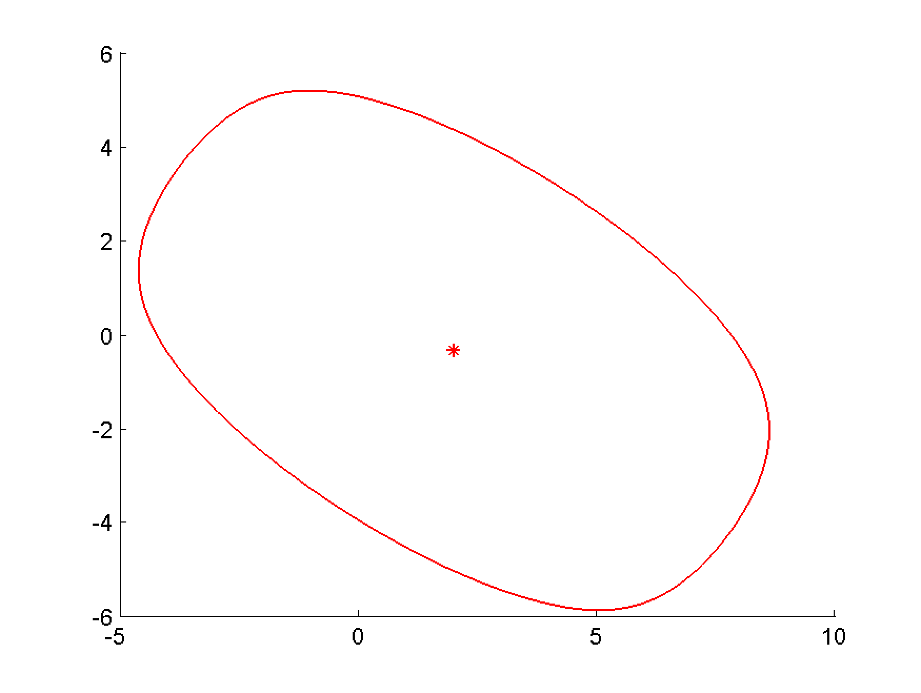
\includegraphics{minksum.png}
\caption{The geometric sum of ellipsoids.}\label{chap_implement:minksumpic}\end{figure}

Figure \hyperref[chap_implement:minksumPic]{ \ref*{chap_implement:minksumPic}} displays the geometric sum of ellipsoids. If
the dimension of the space in which the ellipsoids are defined exceeds
$3$, an error is returned. The result of the geometric sum
operation is not generally an ellipsoid, but it can be approximated by
families of external and internal ellipsoids parametrized by the
direction vector:

\begin{Verbatim}[commandchars=\\\{\},numbers=left,firstnumber=1,stepnumber=1]
\PYG{c}{\PYGZpc{} define the set of directions:}
\PYG{c}{\PYGZpc{} columns of matrix dirsMat are vectors in R\PYGZca{}2}
\PYG{n}{dirsMat} \PYG{p}{=} \PYG{p}{[}\PYG{l+m+mi}{1} \PYG{l+m+mi}{0}\PYG{p}{;} \PYG{l+m+mi}{1} \PYG{l+m+mi}{1}\PYG{p}{;} \PYG{l+m+mi}{0} \PYG{l+m+mi}{1}\PYG{p}{;} \PYG{o}{\PYGZhy{}}\PYG{l+m+mi}{1} \PYG{l+m+mi}{1}\PYG{p}{;} \PYG{l+m+mi}{1} \PYG{l+m+mi}{3}\PYG{p}{]}\PYG{o}{\PYGZsq{}}\PYG{p}{;}
\PYG{c}{\PYGZpc{} compute external ellipsoids for the directions in dirsMat}
\PYG{n}{externalEllVec} \PYG{p}{=} \PYG{n}{ellMat}\PYG{p}{.}\PYG{n}{minksum\PYGZus{}ea}\PYG{p}{(}\PYG{n}{dirsMat}\PYG{p}{)} 

\PYG{c}{\PYGZpc{} externalEllVec =}
\PYG{c}{\PYGZpc{} Array of ellipsoids with dimensionality 1x5}

\PYG{c}{\PYGZpc{} compute internal ellipsoids for the directions in dirsMat}
\PYG{n}{internalEllVec} \PYG{p}{=} \PYG{n}{ellMat}\PYG{p}{.}\PYG{n}{minksum\PYGZus{}ia}\PYG{p}{(}\PYG{n}{dirsMat}\PYG{p}{)}  

\PYG{c}{\PYGZpc{} internalEllVec =}
\PYG{c}{\PYGZpc{} Array of ellipsoids with dimensionality 1x5}

\PYG{c}{\PYGZpc{} intersection of external ellipsoids should always contain }
\PYG{c}{\PYGZpc{} the union of internal ellipsoids:}
\PYG{n}{externalEllVec}\PYG{p}{.}\PYG{n}{doesIntersectionContain}\PYG{p}{(}\PYG{n}{internalEllVec}\PYG{p}{,} \PYG{l+s}{\PYGZsq{}}\PYG{l+s}{u\PYGZsq{}}\PYG{p}{)} 
\PYG{c}{\PYGZpc{} }
\PYG{c}{\PYGZpc{} ans =}
\PYG{c}{\PYGZpc{} }
\PYG{c}{\PYGZpc{}      1}
\end{Verbatim}

Functions minksum\_ea and minksum\_ia work for
ellipsoids of arbitrary dimension. They should be used for general
computations whereas minksum is there merely for visualization purposes.

If the geometric difference of two ellipsoids is not an empty set, it
can be computed explicitely and plotted for ellipsoids in
${\bf R}$, ${\bf R}^2$ and ${\bf R}^3$:

\begin{Verbatim}[commandchars=\\\{\},numbers=left,firstnumber=1,stepnumber=1]
\PYG{c}{\PYGZpc{} ellipsoid defined by squeezing the ellipsoid ellMat(2, 2)}
\PYG{n}{fourthEllObj} \PYG{p}{=} \PYG{n}{ellMat}\PYG{p}{(}\PYG{l+m+mi}{2}\PYG{p}{,} \PYG{l+m+mi}{2}\PYG{p}{)}\PYG{p}{.}\PYG{n}{getShape}\PYG{p}{(}\PYG{l+m+mf}{0.4}\PYG{p}{)}\PYG{p}{;}  
\PYG{c}{\PYGZpc{} check if the geometric difference firstEllObj \PYGZhy{} fourthEllObj is nonempty}
\PYG{n}{firstEllObj} \PYG{o}{\PYGZgt{}}\PYG{p}{=} \PYG{n}{fourthEllObj}  
\PYG{c}{\PYGZpc{} }
\PYG{c}{\PYGZpc{} ans =}
\PYG{c}{\PYGZpc{} }
\PYG{c}{\PYGZpc{}      1}

\PYG{c}{\PYGZpc{} compute and plot this geometric difference}
\PYG{n}{firstEllObj}\PYG{p}{.}\PYG{n}{minkdiff}\PYG{p}{(}\PYG{n}{fourthEllObj}\PYG{p}{)}\PYG{p}{;}
\end{Verbatim}
\begin{figure}[htbp]
\centering
\capstart

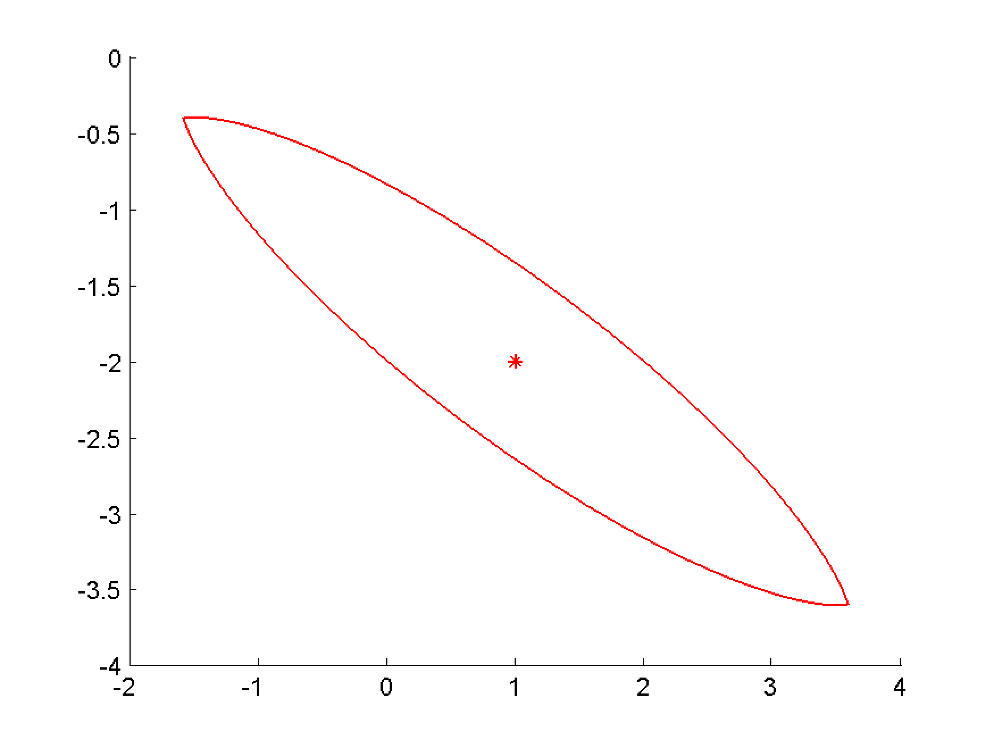
\includegraphics{minkdiff.png}
\caption{The geometric difference of ellipsoids.}\label{chap_implement:minkdiffpic}\end{figure}

Figure \hyperref[chap_implement:minkdiffPic]{ \ref*{chap_implement:minkdiffPic}} shows the geometric difference of ellipsoids.

Similar to minksum, minkdiff is there for visualization purpose. It
works only for dimensions $1$, $2$ and $3$, and for
higher dimensions it returns an error. For arbitrary dimensions, the
geometric difference can be approximated by families of external and
internal ellipsoids parametrized by the direction vector, provided this
direction is not bad:

\begin{Verbatim}[commandchars=\\\{\},numbers=left,firstnumber=1,stepnumber=1]
\PYG{n}{absTol} \PYG{o}{=} \PYG{n}{getAbsTol}\PYG{p}{(}\PYG{n}{firstEllObj}\PYG{p}{)}\PYG{p}{;}
\PYG{o}{\PYGZpc{}} \PYG{n}{find} \PYG{n}{out} \PYG{n}{which} \PYG{n}{of} \PYG{n}{the} \PYG{n}{directions} \PYG{n}{in} \PYG{n}{dirsMat} \PYG{n}{are} \PYG{n}{bad}
\PYG{n}{firstEllObj}\PYG{p}{.}\PYG{n}{isbaddirection}\PYG{p}{(}\PYG{n}{fourthEllObj}\PYG{p}{,} \PYG{n}{dirsMat}\PYG{p}{,} \PYG{n}{absTol}\PYG{p}{)}  

\PYG{o}{\PYGZpc{}} \PYG{n}{ans} \PYG{o}{=}
\PYG{o}{\PYGZpc{}} 
\PYG{o}{\PYGZpc{}}      \PYG{l+m+mi}{1}     \PYG{l+m+mi}{0}     \PYG{l+m+mi}{0}     \PYG{l+m+mi}{1}     \PYG{l+m+mi}{0} 


\PYG{o}{\PYGZpc{}} \PYG{n}{two} \PYG{n}{of} \PYG{n}{five} \PYG{n}{directions} \PYG{n}{specified} \PYG{n}{by} \PYG{n}{dirsMat} \PYG{n}{are} \PYG{n}{bad}\PYG{p}{,}
\PYG{o}{\PYGZpc{}} \PYG{n}{so}\PYG{p}{,} \PYG{n}{only} \PYG{n}{three} \PYG{n}{ellipsoidal} \PYG{n}{approximations} 
\PYG{o}{\PYGZpc{}} \PYG{n}{can} \PYG{n}{be} \PYG{n}{produced} \PYG{k}{for} \PYG{n}{this} \PYG{n}{dirsMat}\PYG{o}{:}
\PYG{n}{externalEllVec} \PYG{o}{=} \PYG{n}{firstEllObj}\PYG{p}{.}\PYG{n}{minkdiff\PYGZus{}ea}\PYG{p}{(}\PYG{n}{fourthEllObj}\PYG{p}{,} \PYG{n}{dirsMat}\PYG{p}{)} 

\PYG{o}{\PYGZpc{}} \PYG{n}{externalEllVec} \PYG{o}{=}
\PYG{o}{\PYGZpc{}} \PYG{n}{Array} \PYG{n}{of} \PYG{n}{ellipsoids} \PYG{n}{with} \PYG{n}{dimensionality} \PYG{l+m+mi}{1}\PYG{n}{x3}

\PYG{n}{internalEllVec} \PYG{o}{=} \PYG{n}{firstEllObj}\PYG{p}{.}\PYG{n}{minkdiff\PYGZus{}ia}\PYG{p}{(}\PYG{n}{fourthEllObj}\PYG{p}{,} \PYG{n}{dirsMat}\PYG{p}{)}

\PYG{o}{\PYGZpc{}} \PYG{n}{internalEllVec} \PYG{o}{=}
\PYG{o}{\PYGZpc{}} \PYG{n}{Array} \PYG{n}{of} \PYG{n}{ellipsoids} \PYG{n}{with} \PYG{n}{dimensionality} \PYG{l+m+mi}{1}\PYG{n}{x3}
\end{Verbatim}

Operation ’difference-sum’ described in section
2.2.4 is implemented in functions minkmp, minkmp\_ea, minkmp\_ia, the
first one of which is used for visualization and works for dimensions
not higher than $3$, whereas the last two can deal with ellipsoids
of arbitrary dimension.

\begin{Verbatim}[commandchars=\\\{\},numbers=left,firstnumber=1,stepnumber=1]
\PYG{c}{\PYGZpc{} ellipsoidal approximations for (firstEllObj \PYGZhy{} thirdEllObj + secEllObj)}

\PYG{c}{\PYGZpc{} external}
\PYG{n}{externalEllVec} \PYG{p}{=} \PYG{n}{firstEllObj}\PYG{p}{.}\PYG{n}{minkmp\PYGZus{}ea}\PYG{p}{(}\PYG{n}{thirdEllObj}\PYG{p}{,} \PYG{n}{secEllObj}\PYG{p}{,} \PYG{n}{dirsMat}\PYG{p}{)} 
\PYG{c}{\PYGZpc{} externalEllVec =}
\PYG{c}{\PYGZpc{} Array of ellipsoids with dimensionality 1x5}

\PYG{c}{\PYGZpc{} internal}
\PYG{n}{internalEllVec} \PYG{p}{=} \PYG{n}{firstEllObj}\PYG{p}{.}\PYG{n}{minkmp\PYGZus{}ia}\PYG{p}{(}\PYG{n}{thirdEllObj}\PYG{p}{,} \PYG{n}{secEllObj}\PYG{p}{,} \PYG{n}{dirsMat}\PYG{p}{)}
\PYG{c}{\PYGZpc{} internalEllVec =}
\PYG{c}{\PYGZpc{} Array of ellipsoids with dimensionality 1x5}

\PYG{c}{\PYGZpc{} plot the set (firstEllObj \PYGZhy{} thirdEllObj + secEllObj)}
\PYG{n}{firstEllObj}\PYG{p}{.}\PYG{n}{minkmp}\PYG{p}{(}\PYG{n}{thirdEllObj}\PYG{p}{,} \PYG{n}{secEllObj}\PYG{p}{)}\PYG{p}{;}
\end{Verbatim}
\begin{figure}[htbp]
\centering
\capstart

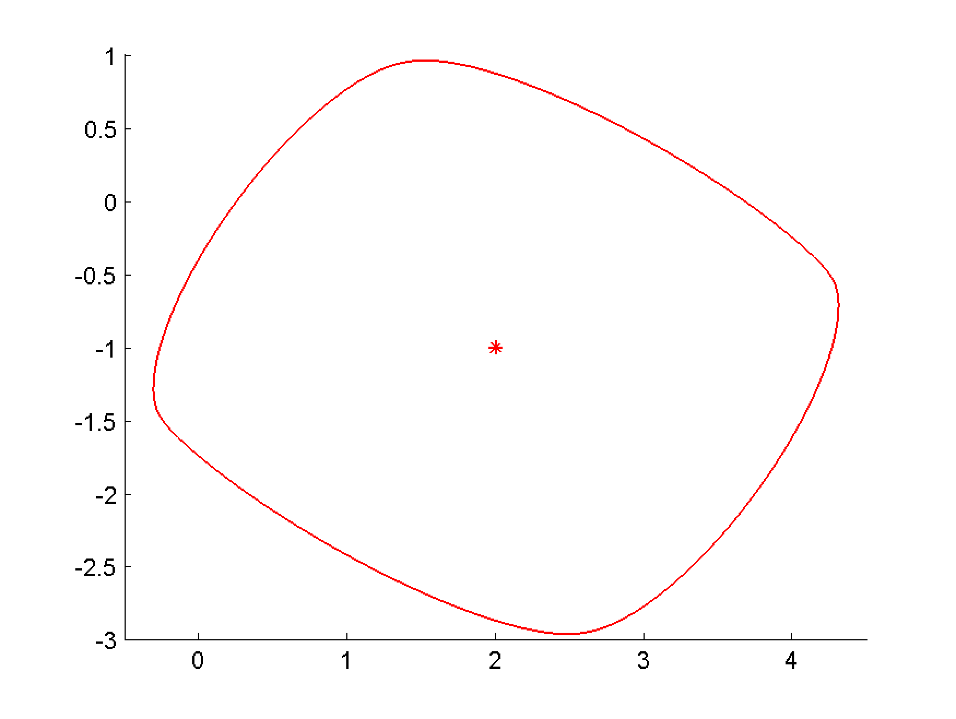
\includegraphics{minkpm.png}
\caption{Implementation of an operation `sum-difference'.}\label{chap_implement:minkpmpic}\end{figure}
\begin{figure}[htbp]
\centering
\capstart

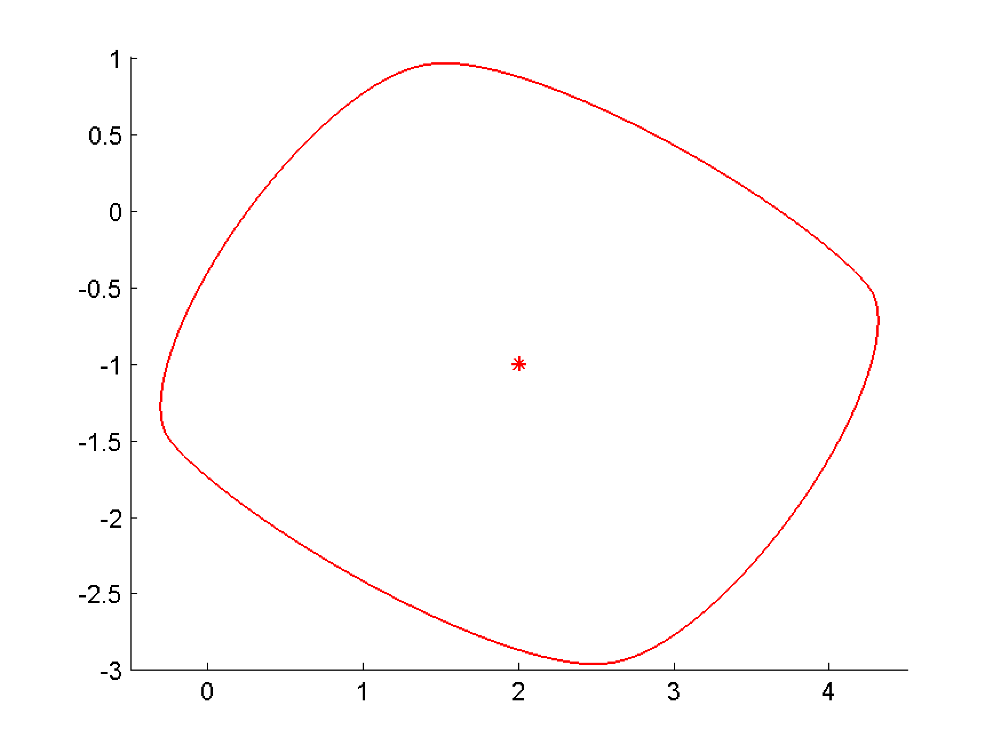
\includegraphics{minkmp.png}
\caption{Implementation of an operation `difference-sum'.}\label{chap_implement:minkmppic}\end{figure}

Figure $\ref{minkPic}$ displays results of
the implementation of minkpm and minkmp operations.

Similarly, operation
’sum-difference’ described in section 2.2.5 is implemented in functions
minkpm, minkpm\_ea, minkpm\_ia, the first one of which is used for
visualization and works for dimensions not higher than $3$,
whereas the last two can deal with ellipsoids of arbitrary dimension.

\begin{Verbatim}[commandchars=\\\{\},numbers=left,firstnumber=1,stepnumber=1]
\PYG{c}{\PYGZpc{} ellipsoidal approximations for (firstEllObj + secEllObj \PYGZhy{} thirdEllObj)}
\PYG{n}{bufEllVec} \PYG{p}{=} \PYG{p}{[}\PYG{n}{firstEllObj} \PYG{n}{secEllObj}\PYG{p}{]}\PYG{p}{;}
\PYG{n}{externalEllVec} \PYG{p}{=} \PYG{n}{bufEllVec}\PYG{p}{.}\PYG{n}{minkpm\PYGZus{}ea}\PYG{p}{(}\PYG{n}{thirdEllObj}\PYG{p}{,} \PYG{n}{dirsMat}\PYG{p}{)}  \PYG{c}{\PYGZpc{} external}

\PYG{c}{\PYGZpc{} externalEllVec =}
\PYG{c}{\PYGZpc{} Array of ellipsoids with dimensionality 1x5}

\PYG{n}{internalEllVec} \PYG{p}{=} \PYG{n}{bufEllVec}\PYG{p}{.}\PYG{n}{minkpm\PYGZus{}ia}\PYG{p}{(}\PYG{n}{thirdEllObj}\PYG{p}{,} \PYG{n}{dirsMat}\PYG{p}{)}  \PYG{c}{\PYGZpc{} internal}

\PYG{c}{\PYGZpc{} internalEllVec =}
\PYG{c}{\PYGZpc{} Array of ellipsoids with dimensionality 1x4}

\PYG{c}{\PYGZpc{} plot the set (firstEllObj + secEllObj \PYGZhy{} thirdEllObj)}
\PYG{n}{firstEllObj}\PYG{p}{.}\PYG{n}{minkpm}\PYG{p}{(}\PYG{n}{secEllObj}\PYG{p}{,} \PYG{n}{thirdEllObj}\PYG{p}{)}
\end{Verbatim}


\section{Operations with hyperplanes}
\label{chap_implement:operations-with-hyperplanes}
The class hyperplane of the \emph{Ellipsoidal Toolbox} is used to describe
hyperplanes and halfspaces. The following two commands define one and
the same hyperplane but two different halfspaces:

\begin{Verbatim}[commandchars=\\\{\},numbers=left,firstnumber=1,stepnumber=1]
\PYG{n}{firstHypObj} \PYG{o}{=} \PYG{n}{hyperplane}\PYG{p}{(}\PYG{p}{[}\PYG{l+m+mi}{1}\PYG{p}{;} \PYG{l+m+mi}{1}\PYG{p}{]}\PYG{p}{,} \PYG{l+m+mi}{1}\PYG{p}{)}\PYG{p}{;}  \PYG{o}{\PYGZpc{}} \PYG{n}{defines} \PYG{n}{halfspace} \PYG{n}{x1} \PYG{o}{+} \PYG{n}{x2} \PYG{o}{\PYGZlt{}}\PYG{o}{=} \PYG{l+m+mi}{1}
\PYG{n}{firstHypObj} \PYG{o}{=} \PYG{n}{hyperplane}\PYG{p}{(}\PYG{p}{[}\PYG{o}{\PYGZhy{}}\PYG{l+m+mi}{1}\PYG{p}{;} \PYG{o}{\PYGZhy{}}\PYG{l+m+mi}{1}\PYG{p}{]}\PYG{p}{,} \PYG{o}{\PYGZhy{}}\PYG{l+m+mi}{1}\PYG{p}{)}\PYG{p}{;}  \PYG{o}{\PYGZpc{}} \PYG{n}{defines} \PYG{n}{halfspace} \PYG{n}{x1} \PYG{o}{+} \PYG{n}{x2} \PYG{o}{\PYGZgt{}}\PYG{o}{=} \PYG{l+m+mi}{1}
\end{Verbatim}

The following functions and operators are overloaded for the hyperplane
class:
\begin{itemize}
\item {} 
isempty(hypObj) -- checks if hypObj is an empty hyperplane.

\item {} 
display(hypObj) -- displays the details of hyperplane
$H(c,\gamma)$, namely, its normal $c$ and the scalar
$\gamma$.

\item {} 
plot(hypObj) -- plots hyperplane $H(c,\gamma)$ if the dimension
of the space in which it is defined is not greater than 3.

\item {} 
firstHypObj == secHypObj -- checks if hyperplanes
$H(c_1,\gamma_1)$ and $H(c_2,\gamma_2)$ are equal.

\item {} 
firstHypObj = secHypObj -- checks if hyperplanes
$H(c_1,\gamma_1)$ and $H(c_2,\gamma_2)$ are not equal.

\item {} 
{[} , {]} -- concatenates the hyperplanes into the horizontal array, e.g. hypVec
= {[}firstHypObj secHypObj thirdHypObj{]}.

\item {} 
{[} ; {]} -- concatenates the hyperplanes into the vertical array, e.g. hypMat =
{[}firstHypObj secHypObj; thirdHypObj fourthHypObj{]} -- defines
$2\times 2$ array of hyperplanes.

\item {} 
-hypObj -- defines hyperplane $H(-c,-\gamma)$, which is the same
as $H(c,\gamma)$ but specifies different halfspace.

\end{itemize}

There are several ways to access the internal data of the hyperplane
object:

\begin{Verbatim}[commandchars=\\\{\},numbers=left,firstnumber=1,stepnumber=1]
\PYG{p}{[}\PYG{n}{normVec}\PYG{p}{,} \PYG{n}{hypScal}\PYG{p}{]} \PYG{o}{=} \PYG{n}{firstHypObj}\PYG{p}{.}\PYG{k+kt}{double}\PYG{p}{(}\PYG{p}{)}

\PYG{o}{\PYGZpc{}} \PYG{n}{normVec} \PYG{o}{=}
\PYG{o}{\PYGZpc{}} 
\PYG{o}{\PYGZpc{}}    \PYG{o}{\PYGZhy{}}\PYG{l+m+mi}{1}
\PYG{o}{\PYGZpc{}}    \PYG{o}{\PYGZhy{}}\PYG{l+m+mi}{1}
\PYG{o}{\PYGZpc{}} 
\PYG{o}{\PYGZpc{}} \PYG{n}{hypScal} \PYG{o}{=}
\PYG{o}{\PYGZpc{}} 
\PYG{o}{\PYGZpc{}}    \PYG{o}{\PYGZhy{}}\PYG{l+m+mi}{1}
\end{Verbatim}

\begin{Verbatim}[commandchars=\\\{\},numbers=left,firstnumber=1,stepnumber=1]
\PYG{n}{firstHypObj}\PYG{p}{.}\PYG{n}{dimension}\PYG{p}{(}\PYG{p}{)}

\PYG{o}{\PYGZpc{}} \PYG{n}{ans} \PYG{o}{=}
\PYG{o}{\PYGZpc{}} 
\PYG{o}{\PYGZpc{}}      \PYG{l+m+mi}{2}
\end{Verbatim}

\begin{Verbatim}[commandchars=\\\{\},numbers=left,firstnumber=1,stepnumber=1]
\PYG{c}{\PYGZpc{} define two hyperplanes passing through the origin}
\PYG{n}{secHypObj} \PYG{p}{=} \PYG{n}{hyperplane}\PYG{p}{(}\PYG{p}{[}\PYG{l+m+mi}{1} \PYG{o}{\PYGZhy{}}\PYG{l+m+mi}{1}\PYG{p}{;} \PYG{l+m+mi}{1} \PYG{l+m+mi}{1}\PYG{p}{]}\PYG{p}{)}\PYG{p}{;} 
\PYG{n}{firstHypObj}\PYG{p}{.}\PYG{n}{isparallel}\PYG{p}{(}\PYG{n}{secHypObj}\PYG{p}{)} 

\PYG{c}{\PYGZpc{} ans =}
\PYG{c}{\PYGZpc{} }
\PYG{c}{\PYGZpc{}      1     0}
\end{Verbatim}

All the functions of \emph{Ellipsoidal Toolbox} that accept
hyperplane object as parameter, work with single hyperplanes as well as
with hyperplane arrays. One exception is the function parameters that
allows only single hyperplane object.

An array of hyperplanes can be converted to the polytope object of the
Multi-Parametric Toolbox (Kvasnica et al. (2004), (“Multi-Parametric
Toolbox Homepage”)), and back:

\begin{Verbatim}[commandchars=\\\{\},numbers=left,firstnumber=1,stepnumber=1]
\PYG{c}{\PYGZpc{}define array of four hyperplanes:}
\PYG{n}{hypVec} \PYG{p}{=} \PYG{n}{hyperplane}\PYG{p}{(}\PYG{p}{[}\PYG{l+m+mi}{1} \PYG{l+m+mi}{1}\PYG{p}{;} \PYG{o}{\PYGZhy{}}\PYG{l+m+mi}{1} \PYG{o}{\PYGZhy{}}\PYG{l+m+mi}{1}\PYG{p}{;} \PYG{l+m+mi}{1} \PYG{o}{\PYGZhy{}}\PYG{l+m+mi}{1}\PYG{p}{;} \PYG{o}{\PYGZhy{}}\PYG{l+m+mi}{1} \PYG{l+m+mi}{1}\PYG{p}{]}\PYG{o}{\PYGZsq{}}\PYG{p}{,} \PYG{p}{[}\PYG{l+m+mi}{2} \PYG{l+m+mi}{2} \PYG{l+m+mi}{2} \PYG{l+m+mi}{2}\PYG{p}{]}\PYG{p}{)}

\PYG{c}{\PYGZpc{} array of hyperplanes: }
\PYG{c}{\PYGZpc{} size: [1 4]}
\PYG{c}{\PYGZpc{} }
\PYG{c}{\PYGZpc{} Element: [1 1]}
\PYG{c}{\PYGZpc{} Normal:}
\PYG{c}{\PYGZpc{}      1}
\PYG{c}{\PYGZpc{}      1}
\PYG{c}{\PYGZpc{} }
\PYG{c}{\PYGZpc{} Shift:}
\PYG{c}{\PYGZpc{}      2}
\PYG{c}{\PYGZpc{} }
\PYG{c}{\PYGZpc{} Hyperplane in R\PYGZca{}2.}
\PYG{c}{\PYGZpc{} }
\PYG{c}{\PYGZpc{} }
\PYG{c}{\PYGZpc{} Element: [1 2]}
\PYG{c}{\PYGZpc{} Normal:}
\PYG{c}{\PYGZpc{}     \PYGZhy{}1}
\PYG{c}{\PYGZpc{}     \PYGZhy{}1}
\PYG{c}{\PYGZpc{} }
\PYG{c}{\PYGZpc{} Shift:}
\PYG{c}{\PYGZpc{}      2}
\PYG{c}{\PYGZpc{} }
\PYG{c}{\PYGZpc{} Hyperplane in R\PYGZca{}2.}
\PYG{c}{\PYGZpc{} }
\PYG{c}{\PYGZpc{} }
\PYG{c}{\PYGZpc{} Element: [1 3]}
\PYG{c}{\PYGZpc{} Normal:}
\PYG{c}{\PYGZpc{}      1}
\PYG{c}{\PYGZpc{}     \PYGZhy{}1}
\PYG{c}{\PYGZpc{} }
\PYG{c}{\PYGZpc{} Shift:}
\PYG{c}{\PYGZpc{}      2}
\PYG{c}{\PYGZpc{} }
\PYG{c}{\PYGZpc{} Hyperplane in R\PYGZca{}2.}
\PYG{c}{\PYGZpc{} }
\PYG{c}{\PYGZpc{} }
\PYG{c}{\PYGZpc{} Element: [1 4]}
\PYG{c}{\PYGZpc{} Normal:}
\PYG{c}{\PYGZpc{}     \PYGZhy{}1}
\PYG{c}{\PYGZpc{}      1}
\PYG{c}{\PYGZpc{} }
\PYG{c}{\PYGZpc{} Shift:}
\PYG{c}{\PYGZpc{}      2}
\PYG{c}{\PYGZpc{} }
\PYG{c}{\PYGZpc{} Hyperplane in R\PYGZca{}2.}

\PYG{c}{\PYGZpc{} convert array of hyperplanes to polytope}
\PYG{n}{firstPolObj}  \PYG{p}{=} \PYG{n}{hyperplane2polytope}\PYG{p}{(}\PYG{n}{hypVec}\PYG{p}{)}\PYG{p}{;}
\PYG{c}{\PYGZpc{} covert polytope to array of hyperplanes  }
\PYG{n}{convertedHypVec} \PYG{p}{=} \PYG{n}{polytope2hyperplane}\PYG{p}{(}\PYG{n}{firstPolObj}\PYG{p}{)}\PYG{p}{;}  
\PYG{n}{convertedHypVec} \PYG{o}{==} \PYG{n}{hypVec}

\PYG{c}{\PYGZpc{} ans =}
\PYG{c}{\PYGZpc{} }
\PYG{c}{\PYGZpc{}      1     1     1     1}
\end{Verbatim}

Functions hyperplane2polytope and
polytope2hyperplane require the Multi-Parametric Toolbox to be
installed.

We can compute distance from ellipsoids to hyperplanes and polytopes:

\begin{Verbatim}[commandchars=\\\{\},numbers=left,firstnumber=1,stepnumber=1]
\PYG{c}{\PYGZpc{} distance from ellipsoid firstEllObj to each of the hyperplanes in hypVec}
\PYG{n}{firstEllObj}\PYG{p}{.}\PYG{n}{distance}\PYG{p}{(}\PYG{n}{hypVec}\PYG{p}{)}  

\PYG{c}{\PYGZpc{} ans =}
\PYG{c}{\PYGZpc{} }
\PYG{c}{\PYGZpc{}      \PYGZhy{}0.5176    0.8966   \PYGZhy{}2.6841    0.1444}

\PYG{c}{\PYGZpc{} distance from each of the ellipsoids in ellMat to the polytope}
\PYG{c}{\PYGZpc{} firstPolObj}
\PYG{n}{ellMat}\PYG{p}{.}\PYG{n}{distance}\PYG{p}{(}\PYG{n}{firstPolObj}\PYG{p}{)}  

\PYG{c}{\PYGZpc{} ans =}
\PYG{c}{\PYGZpc{} }
\PYG{c}{\PYGZpc{}      0     0}
\PYG{c}{\PYGZpc{}      0     0}
\end{Verbatim}

A negative distance value in the case of ellipsoid and hyperplane means
that the ellipsoid intersects the hyperplane. As we see in this example,
ellipsoid firstEllObj intersects hyperplanes hypVec(1) and hypVec(3) and
has no common points with hypVec(2) and hypVec(4). When distance
function has a polytope as a parameter, it always returns nonnegative
values to be consistent with distance function of the Multi-Parametric
Toolbox. Here, the zero distance values mean that each ellipsoid in
ellMat has nonempty intersection with polytope firstPolObj.

It can be checked if the union or intersection of given ellipsoids
intersects given hyperplanes or polytopes:

\begin{Verbatim}[commandchars=\\\{\},numbers=left,firstnumber=1,stepnumber=1]
\PYG{n}{ellMat}\PYG{p}{.}\PYG{n}{intersect}\PYG{p}{(}\PYG{n}{hypVec}\PYG{p}{,} \PYG{l+s+sc}{\PYGZsq{}u\PYGZsq{}}\PYG{p}{)}

\PYG{o}{\PYGZpc{}} \PYG{n}{ans} \PYG{o}{=}
\PYG{o}{\PYGZpc{}} 
\PYG{o}{\PYGZpc{}}      \PYG{l+m+mi}{1}     \PYG{l+m+mi}{1}     \PYG{l+m+mi}{1}     \PYG{l+m+mi}{1}
\end{Verbatim}

\begin{Verbatim}[commandchars=\\\{\},numbers=left,firstnumber=1,stepnumber=1]
\PYG{n}{ellMat}\PYG{p}{(}\PYG{o}{:}\PYG{p}{,} \PYG{l+m+mi}{1}\PYG{p}{)}\PYG{p}{.}\PYG{n}{intersect}\PYG{p}{(}\PYG{n}{hypVec}\PYG{p}{,} \PYG{l+s+sc}{\PYGZsq{}i\PYGZsq{}}\PYG{p}{)}

\PYG{o}{\PYGZpc{}} \PYG{n}{ans} \PYG{o}{=}
\PYG{o}{\PYGZpc{}} 
\PYG{o}{\PYGZpc{}}      \PYG{l+m+mi}{0}     \PYG{l+m+mi}{0}     \PYG{l+m+mi}{1}     \PYG{l+m+mi}{0}
\end{Verbatim}

\begin{Verbatim}[commandchars=\\\{\},numbers=left,firstnumber=1,stepnumber=1]
\PYG{n}{bufEllVec} \PYG{o}{=} \PYG{p}{[}\PYG{n}{firstEllObj} \PYG{n}{secEllObj} \PYG{n}{thirdEllObj}\PYG{p}{]}\PYG{p}{;}
\PYG{n}{bufEllVec}\PYG{p}{.}\PYG{n}{intersect}\PYG{p}{(}\PYG{n}{firstPolObj}\PYG{p}{,} \PYG{l+s+sc}{\PYGZsq{}i\PYGZsq{}}\PYG{p}{)}

\PYG{o}{\PYGZpc{}} \PYG{n}{ans} \PYG{o}{=}
\PYG{o}{\PYGZpc{}} 
\PYG{o}{\PYGZpc{}}      \PYG{l+m+mi}{1}
\end{Verbatim}

The intersection of ellipsoid and hyperplane can be computed exactly:

\begin{Verbatim}[commandchars=\\\{\},numbers=left,firstnumber=1,stepnumber=1]
\PYG{c}{\PYGZpc{} compute the intersections of ellipsoids in the second column of ellMat}
\PYG{c}{\PYGZpc{} with hyperplane firstHypObj: }

\PYG{n}{intersectEllMat} \PYG{p}{=} \PYG{n}{ellMat}\PYG{p}{(}\PYG{p}{:}\PYG{p}{,} \PYG{l+m+mi}{2}\PYG{p}{)}\PYG{p}{.}\PYG{n}{hpintersection}\PYG{p}{(}\PYG{n}{firstHypObj}\PYG{p}{)}

\PYG{c}{\PYGZpc{} intersectEllMat =}
\PYG{c}{\PYGZpc{} Array of ellipsoids with dimensionality 2x1}

\PYG{n}{intersectEllMat}\PYG{p}{.}\PYG{n}{isdegenerate}\PYG{p}{(}\PYG{p}{)}  \PYG{c}{\PYGZpc{} resulting ellipsoids should lose rank}

\PYG{c}{\PYGZpc{} ans =}
\PYG{c}{\PYGZpc{} }
\PYG{c}{\PYGZpc{}      1}
\PYG{c}{\PYGZpc{}      1}
\end{Verbatim}

Functions intersection\_ea and intersection\_ia can be used with
hyperplane objects, which in this case define halfspaces and polytope
objects:

\begin{Verbatim}[commandchars=\\\{\},numbers=left,firstnumber=1,stepnumber=1]
\PYG{c}{\PYGZpc{} compute external and internal ellipsoidal approximations}
\PYG{c}{\PYGZpc{} of the intersections of ellipsoids in the first column of ellMat}
\PYG{c}{\PYGZpc{} with the halfspace x1 \PYGZhy{} x2 \PYGZlt{}= 2:}

\PYG{c}{\PYGZpc{} get external ellipsoids}
\PYG{n}{firstExternalEllMat} \PYG{p}{=} \PYG{n}{ellMat}\PYG{p}{(}\PYG{p}{:}\PYG{p}{,} \PYG{l+m+mi}{1}\PYG{p}{)}\PYG{p}{.}\PYG{n}{intersection\PYGZus{}ea}\PYG{p}{(}\PYG{n}{firstHypObj}\PYG{p}{(}\PYG{l+m+mi}{1}\PYG{p}{)}\PYG{p}{)}  
\PYG{c}{\PYGZpc{} firstExternalEllMat =}
\PYG{c}{\PYGZpc{} Array of ellipsoids with dimensionality 2x1}

\PYG{c}{\PYGZpc{} get internal ellipsoids}
\PYG{n}{firstInternalEllMat} \PYG{p}{=} \PYG{n}{ellMat}\PYG{p}{(}\PYG{p}{:}\PYG{p}{,} \PYG{l+m+mi}{1}\PYG{p}{)}\PYG{p}{.}\PYG{n}{intersection\PYGZus{}ia}\PYG{p}{(}\PYG{n}{firstHypObj}\PYG{p}{(}\PYG{l+m+mi}{1}\PYG{p}{)}\PYG{p}{)}  
\PYG{c}{\PYGZpc{} firstInternalEllMat =}
\PYG{c}{\PYGZpc{} Array of ellipsoids with dimensionality 2x1}

\PYG{c}{\PYGZpc{} compute external and internal ellipsoidal approximations}
\PYG{c}{\PYGZpc{} of the intersections of ellipsoids in the first column of ellMat}
\PYG{c}{\PYGZpc{} with the halfspace x1 \PYGZhy{} x2 \PYGZgt{}= 2:}

\PYG{c}{\PYGZpc{} get external ellipsoids}
\PYG{n}{secExternalEllMat} \PYG{p}{=} \PYG{n}{ellMat}\PYG{p}{(}\PYG{p}{:}\PYG{p}{,} \PYG{l+m+mi}{1}\PYG{p}{)}\PYG{p}{.}\PYG{n}{intersection\PYGZus{}ea}\PYG{p}{(}\PYG{o}{\PYGZhy{}}\PYG{n}{firstHypObj}\PYG{p}{(}\PYG{l+m+mi}{1}\PYG{p}{)}\PYG{p}{)}\PYG{p}{;}
  
\PYG{c}{\PYGZpc{} get internal ellipsoids}
\PYG{n}{secInternalEllMat} \PYG{p}{=} \PYG{n}{ellMat}\PYG{p}{(}\PYG{p}{:}\PYG{p}{,} \PYG{l+m+mi}{1}\PYG{p}{)}\PYG{p}{.}\PYG{n}{intersection\PYGZus{}ia}\PYG{p}{(}\PYG{o}{\PYGZhy{}}\PYG{n}{firstHypObj}\PYG{p}{(}\PYG{l+m+mi}{1}\PYG{p}{)}\PYG{p}{)}\PYG{p}{;}  
\PYG{c}{\PYGZpc{} compute ellipsoidal approximations of the intersection}
\PYG{c}{\PYGZpc{} of ellipsoid firstEll and polytope firstPol:}

\PYG{c}{\PYGZpc{} get external ellipsoid}
\PYG{n}{externalEllMat} \PYG{p}{=} \PYG{n}{ellMat}\PYG{p}{(}\PYG{p}{:}\PYG{p}{,} \PYG{l+m+mi}{1}\PYG{p}{)}\PYG{p}{.}\PYG{n}{intersection\PYGZus{}ea}\PYG{p}{(}\PYG{n}{firstPolObj}\PYG{p}{)}\PYG{p}{;}
\PYG{c}{\PYGZpc{} get internal ellipsoid}
\PYG{n}{internalEllMat} \PYG{p}{=} \PYG{n}{ellMat}\PYG{p}{(}\PYG{p}{:}\PYG{p}{,} \PYG{l+m+mi}{1}\PYG{p}{)}\PYG{p}{.}\PYG{n}{intersection\PYGZus{}ia}\PYG{p}{(}\PYG{n}{firstPolObj}\PYG{p}{)}\PYG{p}{;}
\end{Verbatim}

Function isInside can be used to check if a polytope or union of
polytopes is contained in the intersection of given ellipsoids:

\begin{Verbatim}[commandchars=\\\{\},numbers=left,firstnumber=1,stepnumber=1]
\PYG{c}{\PYGZpc{} polytope secPolObj is obtained by affine transformation of firstPolObj}
\PYG{n}{secPolObj} \PYG{p}{=} \PYG{l+m+mf}{0.5}\PYG{o}{*}\PYG{n}{firstPolObj} \PYG{o}{+} \PYG{p}{[}\PYG{l+m+mi}{1}\PYG{p}{;} \PYG{l+m+mi}{1}\PYG{p}{]}\PYG{p}{;}  

\PYG{c}{\PYGZpc{} check if the intersection of ellipsoids in the first column of ellMat}
\PYG{c}{\PYGZpc{} contains the union of polytopes firstPolObj and secPolObj:}

\PYG{c}{\PYGZpc{} equivalent to: doesIntersectionContain(ellMat(:, 1), firstPolObj \textbar{} secPolObj)}
\PYG{n}{ellMat}\PYG{p}{(}\PYG{p}{:}\PYG{p}{,} \PYG{l+m+mi}{1}\PYG{p}{)}\PYG{p}{.}\PYG{n}{doesIntersectionContain}\PYG{p}{(}\PYG{p}{[}\PYG{n}{firstPolObj} \PYG{n}{secPolObj}\PYG{p}{]}\PYG{p}{)}  

\PYG{c}{\PYGZpc{} ans =}
\PYG{c}{\PYGZpc{} }
\PYG{c}{\PYGZpc{}      0}
\end{Verbatim}

\begin{Verbatim}[commandchars=\\\{\},numbers=left,firstnumber=1,stepnumber=1]
\PYG{c}{\PYGZpc{} equivalent to: doesIntersectionContain(ellMat(2, 2),...}
\PYG{c}{\PYGZpc{}                                  firstPolObj \PYGZam{} secPolObj)}
\PYG{n}{ellMat}\PYG{p}{(}\PYG{l+m+mi}{2}\PYG{p}{,} \PYG{l+m+mi}{2}\PYG{p}{)}\PYG{p}{.}\PYG{n}{doesIntersectionContain}\PYG{p}{(}\PYG{p}{[}\PYG{n}{firstPolObj} \PYG{n}{secPolObj}\PYG{p}{]}\PYG{p}{,} \PYG{l+s}{\PYGZsq{}}\PYG{l+s}{i\PYGZsq{}}\PYG{p}{)}  

\PYG{c}{\PYGZpc{} ans =}
\PYG{c}{\PYGZpc{} }
\PYG{c}{\PYGZpc{}      1}
\end{Verbatim}

Functions distance, intersect, intersection\_ia and isInside use the CVX
interface ( (“CVX Homepage”)) to the external optimization package. The
default optimization package included in the distribution of the
\emph{Ellipsoidal Toolbox} is SeDuMi (Sturm (1999), (“SeDuMi Homepage”)).


\section{Operations with ellipsoidal tubes}
\label{chap_implement:operations-with-ellipsoidal-tubes}
There are several classes in \emph{Ellipsoidal Toolbox} for operations with
ellipsoidal tubes. The class gras.ellapx.smartdb.rels.EllTube is used to
describe ellipsoidal tubes. The class
gras.ellapx.smartdb.rels.EllUnionTube is used to store tubes by the
instant of time:
\begin{gather}
\begin{split}{\mathcal X}_{U}[t]=\bigcup \limits_{\tau\leqslant t}{\mathcal X}[\tau],\end{split}\notag\\\begin{split}\end{split}\notag
\end{gather}
where ${\mathcal X}[\tau]$ is single ellipsoidal tube. The class
gras.ellapx.smartdb.rels.EllTubeProj is used to describe the projection
of the ellipsoidal tubes onto time dependent subspaces.There are two
types of projection: static and dynamic. Also there is class
gras.ellapx.smartdb.rels.EllUnionTubeStaticProj for description of the
projection on static plane tubes by the instant of time. Next we provide
some examples of the operations with ellipsoidal tubes.

\begin{Verbatim}[commandchars=\\\{\},numbers=left,firstnumber=1,stepnumber=1]
\PYG{n}{nPoints}\PYG{o}{=}\PYG{l+m+mi}{5}\PYG{p}{;}
\PYG{n}{calcPrecision}\PYG{o}{=}\PYG{l+m+mf}{0.001}\PYG{p}{;}
\PYG{n}{approxSchemaDescr}\PYG{o}{=}\PYG{k+kt}{char}\PYG{p}{.}\PYG{n}{empty}\PYG{p}{(}\PYG{l+m+mi}{1}\PYG{p}{,}\PYG{l+m+mi}{0}\PYG{p}{)}\PYG{p}{;}
\PYG{n}{approxSchemaName}\PYG{o}{=}\PYG{k+kt}{char}\PYG{p}{.}\PYG{n}{empty}\PYG{p}{(}\PYG{l+m+mi}{1}\PYG{p}{,}\PYG{l+m+mi}{0}\PYG{p}{)}\PYG{p}{;}
\PYG{n}{nDims}\PYG{o}{=}\PYG{l+m+mi}{3}\PYG{p}{;}
\PYG{n}{nTubes}\PYG{o}{=}\PYG{l+m+mi}{1}\PYG{p}{;}
\PYG{n}{lsGoodDirVec}\PYG{o}{=}\PYG{p}{[}\PYG{l+m+mi}{1}\PYG{p}{;}\PYG{l+m+mi}{0}\PYG{p}{;}\PYG{l+m+mi}{1}\PYG{p}{]}\PYG{p}{;}
\PYG{n}{aMat}\PYG{o}{=}\PYG{n}{zeros}\PYG{p}{(}\PYG{n}{nDims}\PYG{p}{,}\PYG{n}{nPoints}\PYG{p}{)}\PYG{p}{;}
\PYG{n}{timeVec}\PYG{o}{=}\PYG{l+m+mi}{1}\PYG{o}{:}\PYG{n}{nPoints}\PYG{p}{;}
\PYG{n}{sTime}\PYG{o}{=}\PYG{n}{nPoints}\PYG{p}{;}
\PYG{n}{approxType}\PYG{o}{=}\PYG{n}{gras}\PYG{p}{.}\PYG{n}{ellapx}\PYG{p}{.}\PYG{n}{enums}\PYG{p}{.}\PYG{n}{EApproxType}\PYG{p}{.}\PYG{n}{Internal}\PYG{p}{;}
\PYG{n}{qArrayList}\PYG{o}{=}\PYG{n}{repmat}\PYG{p}{(}\PYG{p}{\PYGZob{}}\PYG{n}{repmat}\PYG{p}{(}\PYG{n}{diag}\PYG{p}{(}\PYG{p}{[}\PYG{l+m+mi}{1} \PYG{l+m+mi}{2} \PYG{l+m+mi}{3}\PYG{p}{]}\PYG{p}{)}\PYG{p}{,}\PYG{p}{[}\PYG{l+m+mi}{1}\PYG{p}{,}\PYG{l+m+mi}{1}\PYG{p}{,}\PYG{n}{nPoints}\PYG{p}{]}\PYG{p}{)}\PYG{p}{\PYGZcb{}}\PYG{p}{,}\PYG{l+m+mi}{1}\PYG{p}{,}\PYG{n}{nTubes}\PYG{p}{)}\PYG{p}{;}
\PYG{n}{ltGoodDirArray}\PYG{o}{=}\PYG{n}{repmat}\PYG{p}{(}\PYG{n}{lsGoodDirVec}\PYG{p}{,}\PYG{p}{[}\PYG{l+m+mi}{1}\PYG{p}{,}\PYG{n}{nTubes}\PYG{p}{,}\PYG{n}{nPoints}\PYG{p}{]}\PYG{p}{)}\PYG{p}{;}
\PYG{n}{fromMatEllTube}\PYG{o}{=}\PYG{n}{gras}\PYG{p}{.}\PYG{n}{ellapx}\PYG{p}{.}\PYG{n}{smartdb}\PYG{p}{.}\PYG{n}{rels}\PYG{p}{.}\PYG{n}{EllTube}\PYG{p}{.}\PYG{n}{fromQArrays}\PYG{p}{(}\PYG{n}{qArrayList}\PYG{p}{,}\PYG{p}{.}\PYG{p}{.}\PYG{p}{.}
                \PYG{n}{aMat}\PYG{p}{,} \PYG{n}{timeVec}\PYG{p}{,}\PYG{n}{ltGoodDirArray}\PYG{p}{,} \PYG{n}{sTime}\PYG{p}{,} \PYG{n}{approxType}\PYG{p}{,}\PYG{p}{.}\PYG{p}{.}\PYG{p}{.}
                \PYG{n}{approxSchemaName}\PYG{p}{,} \PYG{n}{approxSchemaDescr}\PYG{p}{,} \PYG{n}{calcPrecision}\PYG{p}{)}\PYG{p}{;}
\end{Verbatim}

\begin{Verbatim}[commandchars=\\\{\},numbers=left,firstnumber=1,stepnumber=1]
\PYG{n}{ellArray}\PYG{p}{(}\PYG{n}{nPoints}\PYG{p}{)} \PYG{o}{=} \PYG{n}{ellipsoid}\PYG{p}{(}\PYG{p}{)}\PYG{p}{;}
\PYG{n}{approxType}\PYG{o}{=}\PYG{n}{gras}\PYG{p}{.}\PYG{n}{ellapx}\PYG{p}{.}\PYG{n}{enums}\PYG{p}{.}\PYG{n}{EApproxType}\PYG{p}{.}\PYG{n}{Internal}\PYG{p}{;}
\PYG{n}{sTime}\PYG{o}{=} \PYG{l+m+mi}{2}\PYG{p}{;}
\PYG{k}{for} \PYG{n}{iElem} \PYG{o}{=} \PYG{l+m+mi}{1}\PYG{o}{:}\PYG{n}{nPoints}
   \PYG{n}{ellArray}\PYG{p}{(}\PYG{n}{iElem}\PYG{p}{)} \PYG{o}{=} \PYG{n}{ellipsoid}\PYG{p}{(}\PYG{p}{.}\PYG{p}{.}\PYG{p}{.}
   \PYG{n}{aMat}\PYG{p}{(}\PYG{o}{:}\PYG{p}{,}\PYG{n}{iElem}\PYG{p}{)}\PYG{p}{,} \PYG{n}{qArrayList}\PYG{p}{\PYGZob{}}\PYG{l+m+mi}{1}\PYG{p}{\PYGZcb{}}\PYG{p}{(}\PYG{o}{:}\PYG{p}{,}\PYG{o}{:}\PYG{p}{,}\PYG{n}{iElem}\PYG{p}{)}\PYG{p}{)}\PYG{p}{;} 
\PYG{n}{end}
\PYG{n}{fromEllArrayEllTube} \PYG{o}{=} \PYG{n}{gras}\PYG{p}{.}\PYG{n}{ellapx}\PYG{p}{.}\PYG{n}{smartdb}\PYG{p}{.}\PYG{n}{rels}\PYG{p}{.}\PYG{n}{EllTube}\PYG{p}{.}\PYG{n}{fromEllArray}\PYG{p}{(}\PYG{p}{.}\PYG{p}{.}\PYG{p}{.}
                \PYG{n}{ellArray}\PYG{p}{,} \PYG{n}{timeVec}\PYG{p}{,}\PYG{n}{ltGoodDirArray}\PYG{p}{,} \PYG{n}{sTime}\PYG{p}{,} \PYG{n}{approxType}\PYG{p}{,}\PYG{p}{.}\PYG{p}{.}\PYG{p}{.}
                \PYG{n}{approxSchemaName}\PYG{p}{,}\PYG{n}{approxSchemaDescr}\PYG{p}{,} \PYG{n}{calcPrecision}\PYG{p}{)}\PYG{p}{;}
\end{Verbatim}

We may be
interested in the data about ellipsoidal tube in some particular time
interval, smaller than the one for which the ellipsoidal tube was
computed, say $2\leqslant t\leqslant4$. This data can be extracted
by the cut function:

\begin{Verbatim}[commandchars=\\\{\},numbers=left,firstnumber=1,stepnumber=1]
\PYG{n}{cutTimeVec} \PYG{o}{=} \PYG{p}{[}\PYG{l+m+mi}{2}\PYG{p}{,} \PYG{l+m+mi}{4}\PYG{p}{]}\PYG{p}{;}
\PYG{n}{cutEllTube} \PYG{o}{=} \PYG{n}{fromMatEllTube}\PYG{p}{.}\PYG{n}{cut}\PYG{p}{(}\PYG{n}{cutTimeVec}\PYG{p}{)}\PYG{p}{;}
\end{Verbatim}

\begin{Verbatim}[commandchars=\\\{\},numbers=left,firstnumber=1,stepnumber=1]
\PYG{k+kd}{function} \PYG{n+nx}{example}
   \PYG{n+nx}{aMat} \PYG{o}{=} \PYG{c+cp}{[}\PYG{l+m+mi}{0} \PYG{l+m+mi}{1}\PYG{p}{;} \PYG{l+m+mi}{0} \PYG{l+m+mi}{0}\PYG{c+cp}{]}\PYG{p}{;} \PYG{n+nx}{bMat} \PYG{o}{=} \PYG{n+nx}{eye}\PYG{p}{(}\PYG{l+m+mi}{2}\PYG{p}{)}\PYG{p}{;}  
   \PYG{n+nx}{SUBounds} \PYG{o}{=} \PYG{n+nx}{struct}\PYG{p}{(}\PYG{p}{)}\PYG{p}{;}
   \PYG{n+nx}{SUBounds}\PYG{p}{.}\PYG{n+nx}{center} \PYG{o}{=} \PYG{p}{\PYGZob{}}\PYG{l+s+s1}{\PYGZsq{}sin(t)\PYGZsq{}}\PYG{p}{;} \PYG{l+s+s1}{\PYGZsq{}cos(t)\PYGZsq{}}\PYG{p}{\PYGZcb{}}\PYG{p}{;}  
   \PYG{n+nx}{SUBounds}\PYG{p}{.}\PYG{n+nx}{shape} \PYG{o}{=} \PYG{c+cp}{[}\PYG{l+m+mi}{9} \PYG{l+m+mi}{0}\PYG{p}{;} \PYG{l+m+mi}{0} \PYG{l+m+mi}{2}\PYG{c+cp}{]}\PYG{p}{;} 
   \PYG{n+nx}{sys} \PYG{o}{=} \PYG{n+nx}{elltool}\PYG{p}{.}\PYG{n+nx}{linsys}\PYG{p}{.}\PYG{n+nx}{LinSysContinuous}\PYG{p}{(}\PYG{n+nx}{aMat}\PYG{p}{,} \PYG{n+nx}{bMat}\PYG{p}{,} \PYG{n+nx}{SUBounds}\PYG{p}{)}\PYG{p}{;}
   \PYG{n+nx}{x0EllObj} \PYG{o}{=} \PYG{n+nx}{ell\PYGZus{}unitball}\PYG{p}{(}\PYG{l+m+mi}{2}\PYG{p}{)}\PYG{p}{;}
   \PYG{n+nx}{timeVec} \PYG{o}{=} \PYG{c+cp}{[}\PYG{l+m+mi}{0} \PYG{l+m+mi}{10}\PYG{c+cp}{]}\PYG{p}{;} 
   \PYG{n+nx}{dirsMat} \PYG{o}{=} \PYG{c+cp}{[}\PYG{l+m+mi}{1} \PYG{l+m+mi}{0}\PYG{p}{;} \PYG{l+m+mi}{0} \PYG{l+m+mi}{1}\PYG{c+cp}{]}\PYG{l+s+s1}{\PYGZsq{};  }
\PYG{l+s+s1}{   rsObj = elltool.reach.ReachContinuous(sys, x0EllObj, dirsMat, timeVec);}
\PYG{l+s+s1}{   ellTubeObj = rsObj.getEllTubeRel();}
\PYG{l+s+s1}{   projSpaceList = \PYGZob{}}\PYG{c+cp}{[}\PYG{l+m+mi}{1} \PYG{l+m+mi}{0}\PYG{p}{;}\PYG{l+m+mi}{0} \PYG{l+m+mi}{1}\PYG{c+cp}{]}\PYG{l+s+s1}{\PYGZcb{};}
\PYG{l+s+s1}{   projType = gras.ellapx.enums.EProjType.Static;}
\PYG{l+s+s1}{   statEllTubeProj = ellTubeObj.project(projType,projSpaceList,...}
\PYG{l+s+s1}{      @fGetProjMat);}
\PYG{l+s+s1}{   projType = gras.ellapx.enums.EProjType.DynamicAlongGoodCurve;}
\PYG{l+s+s1}{   dynEllTubeProj=ellTubeObj.project(projType,projSpaceList,...}
\PYG{l+s+s1}{      @fGetProjMat);}
\PYG{l+s+s1}{   plObj=smartdb.disp.RelationDataPlotter();}
\PYG{l+s+s1}{   statEllTubeProj.plot(plObj);}
\PYG{l+s+s1}{   dynEllTubeProj.plot(plObj);}

\PYG{l+s+s1}{end}

\PYG{l+s+s1}{function }\PYG{c+cp}{[}\PYG{n+nx}{projOrthMatArray}\PYG{p}{,}\PYG{n+nx}{projOrthMatTransArray}\PYG{c+cp}{]}\PYG{l+s+s1}{=fGetProjMat(projMat,...}
\PYG{l+s+s1}{    timeVec,varargin)}
\PYG{l+s+s1}{  nTimePoints=length(timeVec);}
\PYG{l+s+s1}{  projOrthMatArray=repmat(projMat,}\PYG{c+cp}{[}\PYG{l+m+mi}{1}\PYG{p}{,}\PYG{l+m+mi}{1}\PYG{p}{,}\PYG{n+nx}{nTimePoints}\PYG{c+cp}{]}\PYG{l+s+s1}{);}
\PYG{l+s+s1}{  projOrthMatTransArray=repmat(projMat.\PYGZsq{}}\PYG{p}{,}\PYG{c+cp}{[}\PYG{l+m+mi}{1}\PYG{p}{,}\PYG{l+m+mi}{1}\PYG{p}{,}\PYG{n+nx}{nTimePoints}\PYG{c+cp}{]}\PYG{p}{)}\PYG{p}{;}
 \PYG{n+nx}{end}
\end{Verbatim}

We can compute the projection of the ellipsoidal
tube onto time-dependent subspace.
\begin{figure}[htbp]
\centering
\capstart

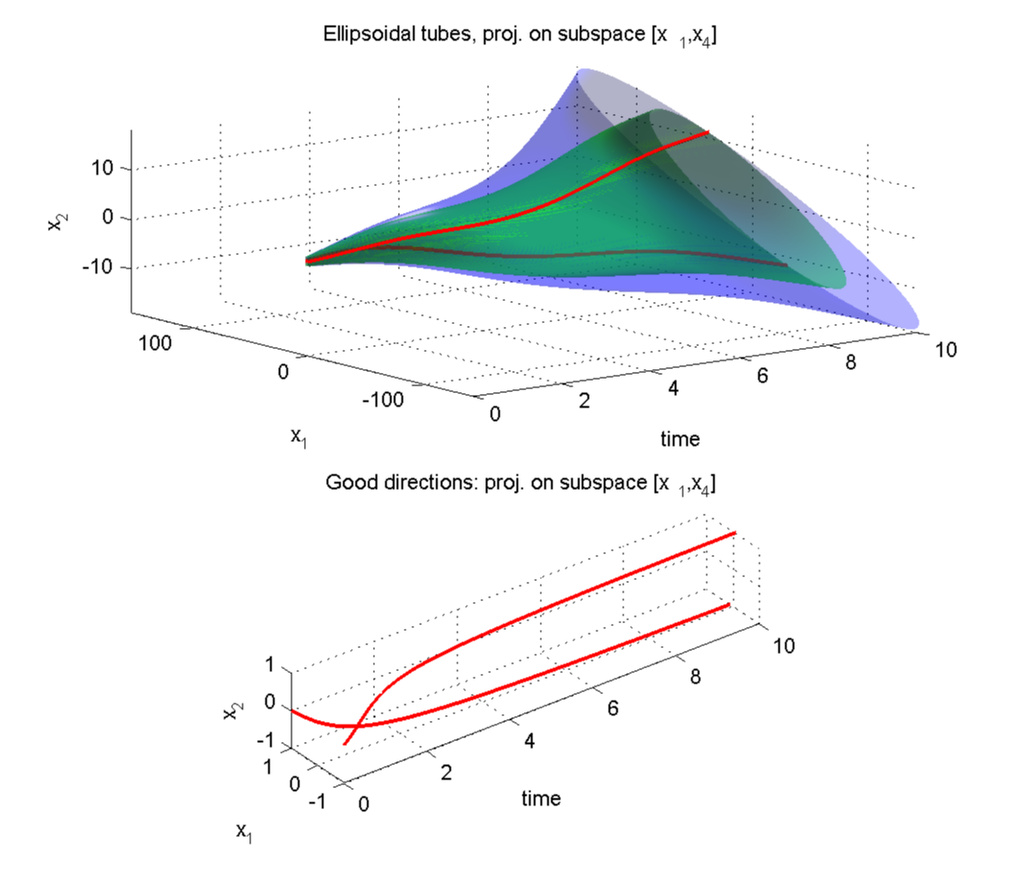
\includegraphics{reachTubeStatProj.png}
\caption{Static projection of the ellipsoidal tube.}\label{chap_implement:stat-proj}\end{figure}
\begin{figure}[htbp]
\centering
\capstart

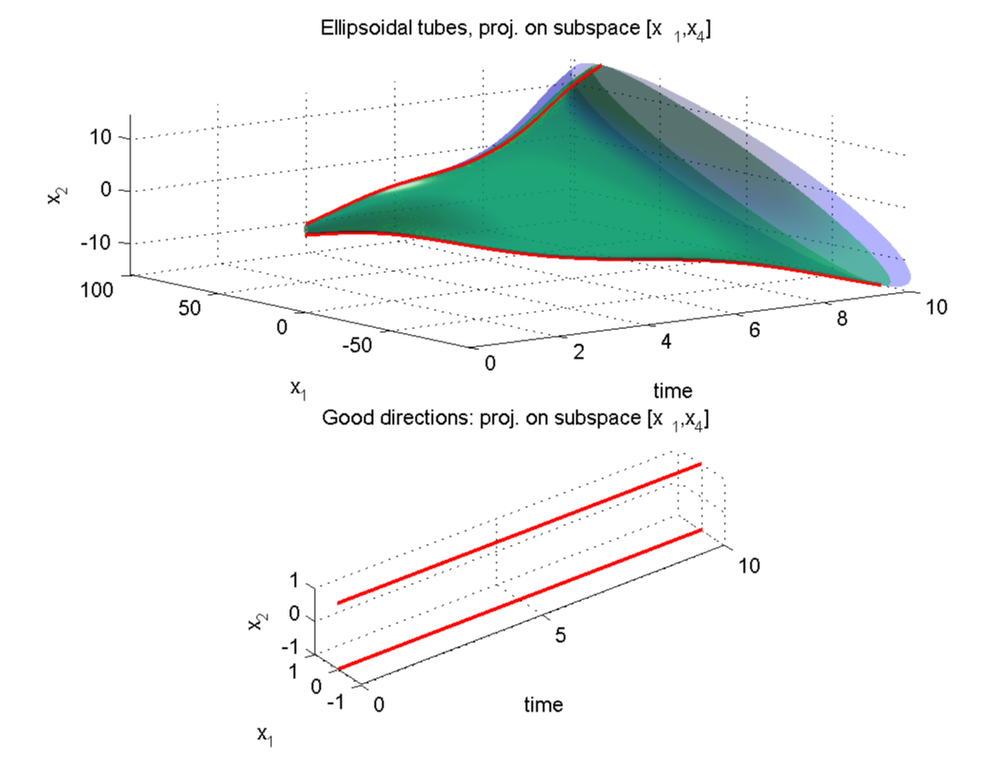
\includegraphics{reachTubeDynProj.png}
\caption{Dynamic projection of the ellipsoidal tube.}\label{chap_implement:dyn-proj}\end{figure}

Figure $\ref{project}$ displays static and dynamic projections.
Also we can see projections of good directions for ellipsoidal tubes.

We can compute tubes by the instant of time using methodfromEllTubes:

\begin{Verbatim}[commandchars=\\\{\},numbers=left,firstnumber=1,stepnumber=1]
\PYG{k+kd}{function} \PYG{n+nx}{example}
   \PYG{n+nx}{aMat} \PYG{o}{=} \PYG{c+cp}{[}\PYG{l+m+mi}{0} \PYG{l+m+mi}{1}\PYG{p}{;} \PYG{l+m+mi}{0} \PYG{l+m+mi}{0}\PYG{c+cp}{]}\PYG{p}{;} \PYG{n+nx}{bMat} \PYG{o}{=} \PYG{n+nx}{eye}\PYG{p}{(}\PYG{l+m+mi}{2}\PYG{p}{)}\PYG{p}{;}  
   \PYG{n+nx}{SUBounds} \PYG{o}{=} \PYG{n+nx}{struct}\PYG{p}{(}\PYG{p}{)}\PYG{p}{;}
   \PYG{n+nx}{SUBounds}\PYG{p}{.}\PYG{n+nx}{center} \PYG{o}{=} \PYG{p}{\PYGZob{}}\PYG{l+s+s1}{\PYGZsq{}sin(t)\PYGZsq{}}\PYG{p}{;} \PYG{l+s+s1}{\PYGZsq{}cos(t)\PYGZsq{}}\PYG{p}{\PYGZcb{}}\PYG{p}{;}  
   \PYG{n+nx}{SUBounds}\PYG{p}{.}\PYG{n+nx}{shape} \PYG{o}{=} \PYG{c+cp}{[}\PYG{l+m+mi}{9} \PYG{l+m+mi}{0}\PYG{p}{;} \PYG{l+m+mi}{0} \PYG{l+m+mi}{2}\PYG{c+cp}{]}\PYG{p}{;} 
   \PYG{n+nx}{sys} \PYG{o}{=} \PYG{n+nx}{elltool}\PYG{p}{.}\PYG{n+nx}{linsys}\PYG{p}{.}\PYG{n+nx}{LinSysContinuous}\PYG{p}{(}\PYG{n+nx}{aMat}\PYG{p}{,} \PYG{n+nx}{bMat}\PYG{p}{,} \PYG{n+nx}{SUBounds}\PYG{p}{)}\PYG{p}{;}
   \PYG{n+nx}{x0EllObj} \PYG{o}{=} \PYG{n+nx}{ell\PYGZus{}unitball}\PYG{p}{(}\PYG{l+m+mi}{2}\PYG{p}{)}\PYG{p}{;}
   \PYG{n+nx}{timeVec} \PYG{o}{=} \PYG{c+cp}{[}\PYG{l+m+mi}{0} \PYG{l+m+mi}{10}\PYG{c+cp}{]}\PYG{p}{;} 
   \PYG{n+nx}{dirsMat} \PYG{o}{=} \PYG{c+cp}{[}\PYG{l+m+mi}{1} \PYG{l+m+mi}{0}\PYG{p}{;} \PYG{l+m+mi}{0} \PYG{l+m+mi}{1}\PYG{c+cp}{]}\PYG{l+s+s1}{\PYGZsq{};  }
\PYG{l+s+s1}{   rsObj = elltool.reach.ReachContinuous(sys, x0EllObj, dirsMat, timeVec);}
\PYG{l+s+s1}{   ellTubeObj = rsObj.getEllTubeRel();}
\PYG{l+s+s1}{   unionEllTube = ...}
\PYG{l+s+s1}{    gras.ellapx.smartdb.rels.EllUnionTube.fromEllTubes(ellTubeObj);}
\PYG{l+s+s1}{   projSpaceList = \PYGZob{}}\PYG{c+cp}{[}\PYG{l+m+mi}{1} \PYG{l+m+mi}{0}\PYG{p}{;}\PYG{l+m+mi}{0} \PYG{l+m+mi}{1}\PYG{c+cp}{]}\PYG{l+s+s1}{\PYGZcb{};}
\PYG{l+s+s1}{   projType = gras.ellapx.enums.EProjType.Static;}
\PYG{l+s+s1}{   statEllTubeProj = unionEllTube.project(projType,projSpaceList,...}
\PYG{l+s+s1}{      @fGetProjMat);}
\PYG{l+s+s1}{   plObj=smartdb.disp.RelationDataPlotter();}
\PYG{l+s+s1}{   statEllTubeProj.plot(plObj);}
\PYG{l+s+s1}{end}

\PYG{l+s+s1}{function }\PYG{c+cp}{[}\PYG{n+nx}{projOrthMatArray}\PYG{p}{,}\PYG{n+nx}{projOrthMatTransArray}\PYG{c+cp}{]}\PYG{l+s+s1}{=fGetProjMat(projMat,...}
\PYG{l+s+s1}{    timeVec,varargin)}
\PYG{l+s+s1}{  nTimePoints=length(timeVec);}
\PYG{l+s+s1}{  projOrthMatArray=repmat(projMat,}\PYG{c+cp}{[}\PYG{l+m+mi}{1}\PYG{p}{,}\PYG{l+m+mi}{1}\PYG{p}{,}\PYG{n+nx}{nTimePoints}\PYG{c+cp}{]}\PYG{l+s+s1}{);}
\PYG{l+s+s1}{  projOrthMatTransArray=repmat(projMat.\PYGZsq{}}\PYG{p}{,}\PYG{c+cp}{[}\PYG{l+m+mi}{1}\PYG{p}{,}\PYG{l+m+mi}{1}\PYG{p}{,}\PYG{n+nx}{nTimePoints}\PYG{c+cp}{]}\PYG{p}{)}\PYG{p}{;}
 \PYG{n+nx}{end}
\end{Verbatim}
\begin{figure}[htbp]
\centering
\capstart

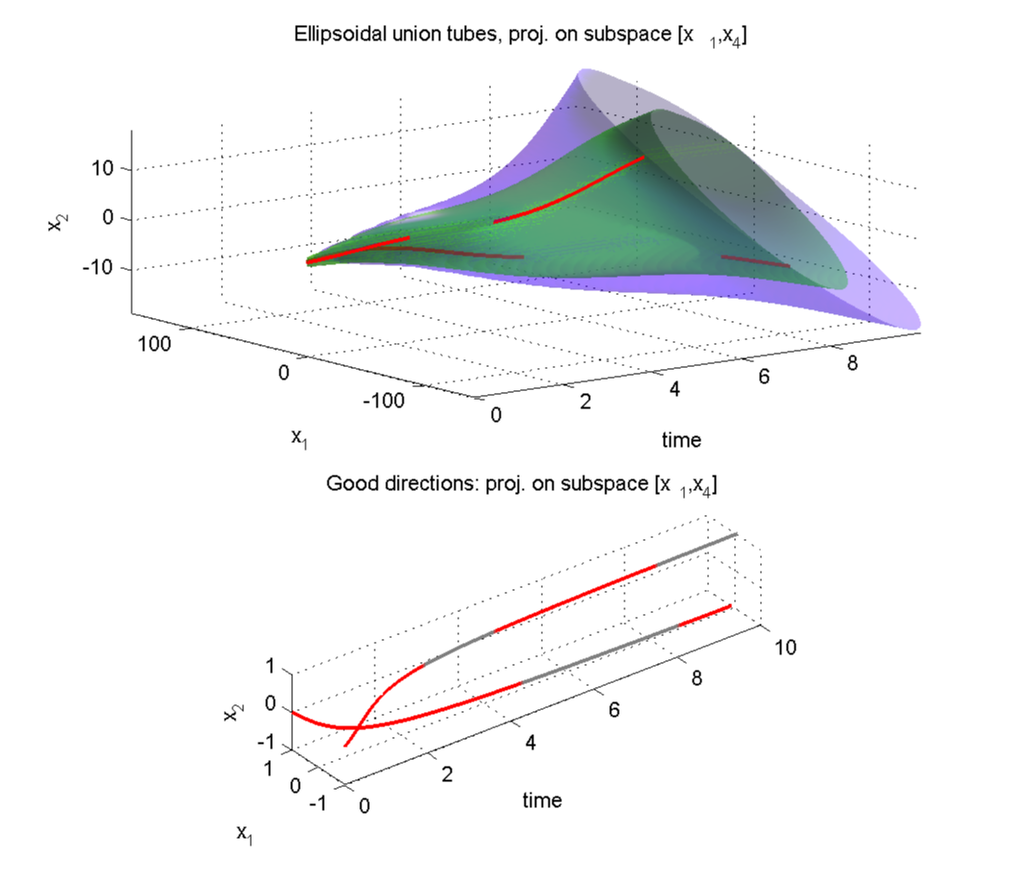
\includegraphics{unionTubeStatProj.png}
\caption{Ellipsoidal tubes by the instant of time.}\label{chap_implement:uniontubestatproj}\end{figure}

Figure \hyperref[chap_implement:unionTubeStatProj]{ \ref*{chap_implement:unionTubeStatProj}} shows projection of ellipsoidal
tubes by the instant of time.

Also we can get initial data from the resulting tube:

\begin{Verbatim}[commandchars=\\\{\},numbers=left,firstnumber=1,stepnumber=1]
\PYG{n}{approxType}\PYG{o}{=}\PYG{n}{gras}\PYG{p}{.}\PYG{n}{ellapx}\PYG{p}{.}\PYG{n}{enums}\PYG{p}{.}\PYG{n}{EApproxType}\PYG{p}{.}\PYG{n}{Internal}\PYG{p}{;}
\PYG{n}{ellArray} \PYG{o}{=} \PYG{n}{fromEllArrayEllTube}\PYG{p}{.}\PYG{n}{getEllArray}\PYG{p}{(}\PYG{n}{approxType}\PYG{p}{)}

\PYG{o}{\PYGZpc{}} \PYG{n}{ellArray} \PYG{o}{=}
\PYG{o}{\PYGZpc{}} \PYG{n}{Array} \PYG{n}{of} \PYG{n}{ellipsoids} \PYG{n}{with} \PYG{n}{dimensionality} \PYG{l+m+mi}{5}\PYG{n}{x1}
\end{Verbatim}

There is a method
to display a content of ellipsoidal tubes.

\begin{Verbatim}[commandchars=\\\{\},numbers=left,firstnumber=1,stepnumber=1]
\PYG{n}{aMat} \PYG{o}{=} \PYG{p}{[}\PYG{l+m+mi}{0} \PYG{l+m+mi}{1}\PYG{p}{;} \PYG{l+m+mi}{0} \PYG{l+m+mi}{0}\PYG{p}{]}\PYG{p}{;} \PYG{n}{bMat} \PYG{o}{=} \PYG{n}{eye}\PYG{p}{(}\PYG{l+m+mi}{2}\PYG{p}{)}\PYG{p}{;}  
\PYG{n}{SUBounds} \PYG{o}{=} \PYG{k}{struct}\PYG{p}{(}\PYG{p}{)}\PYG{p}{;}
\PYG{n}{SUBounds}\PYG{p}{.}\PYG{n}{center} \PYG{o}{=} \PYG{p}{\PYGZob{}}\PYG{err}{\PYGZsq{}}\PYG{n}{sin}\PYG{p}{(}\PYG{n}{t}\PYG{p}{)}\PYG{err}{\PYGZsq{}}\PYG{p}{;} \PYG{err}{\PYGZsq{}}\PYG{n}{cos}\PYG{p}{(}\PYG{n}{t}\PYG{p}{)}\PYG{err}{\PYGZsq{}}\PYG{p}{\PYGZcb{}}\PYG{p}{;}  
\PYG{n}{SUBounds}\PYG{p}{.}\PYG{n}{shape} \PYG{o}{=} \PYG{p}{[}\PYG{l+m+mi}{9} \PYG{l+m+mi}{0}\PYG{p}{;} \PYG{l+m+mi}{0} \PYG{l+m+mi}{2}\PYG{p}{]}\PYG{p}{;} 
\PYG{n}{sys} \PYG{o}{=} \PYG{n}{elltool}\PYG{p}{.}\PYG{n}{linsys}\PYG{p}{.}\PYG{n}{LinSysContinuous}\PYG{p}{(}\PYG{n}{aMat}\PYG{p}{,} \PYG{n}{bMat}\PYG{p}{,} \PYG{n}{SUBounds}\PYG{p}{)}\PYG{p}{;}
\PYG{n}{x0EllObj} \PYG{o}{=} \PYG{n}{ell\PYGZus{}unitball}\PYG{p}{(}\PYG{l+m+mi}{2}\PYG{p}{)}\PYG{p}{;}
\PYG{n}{timeVec} \PYG{o}{=} \PYG{p}{[}\PYG{l+m+mi}{0} \PYG{l+m+mi}{10}\PYG{p}{]}\PYG{p}{;} 
\PYG{k}{for} \PYG{n}{iElem} \PYG{o}{=} \PYG{l+m+mi}{1}\PYG{o}{:}\PYG{l+m+mi}{5}
    \PYG{n}{dirInitial}\PYG{o}{=} \PYG{n}{rand}\PYG{p}{(}\PYG{l+m+mi}{2}\PYG{p}{,} \PYG{l+m+mi}{1}\PYG{p}{)}\PYG{p}{;} 
    \PYG{n}{dirInitial} \PYG{o}{=} \PYG{n}{dirInitial} \PYG{p}{.}\PYG{o}{/} \PYG{n}{norm}\PYG{p}{(}\PYG{n}{dirInitial}\PYG{p}{)}\PYG{p}{;}
    \PYG{n}{dirsMat}\PYG{p}{(}\PYG{o}{:}\PYG{p}{,} \PYG{n}{iElem}\PYG{p}{)} \PYG{o}{=} \PYG{n}{dirInitial}\PYG{p}{;}
\PYG{n}{end}
\PYG{n}{rsObj} \PYG{o}{=} \PYG{n}{elltool}\PYG{p}{.}\PYG{n}{reach}\PYG{p}{.}\PYG{n}{ReachContinuous}\PYG{p}{(}\PYG{n}{sys}\PYG{p}{,} \PYG{n}{x0EllObj}\PYG{p}{,} \PYG{n}{dirsMat}\PYG{p}{,} \PYG{n}{timeVec}\PYG{p}{)}\PYG{p}{;}
\PYG{n}{ellTubeObj} \PYG{o}{=} \PYG{n}{rsObj}\PYG{p}{.}\PYG{n}{getEllTubeRel}\PYG{p}{(}\PYG{p}{)}\PYG{p}{;}
\PYG{n}{ellTubeObj}\PYG{p}{.}\PYG{n}{dispOnUI}\PYG{p}{(}\PYG{p}{)}\PYG{p}{;}
\end{Verbatim}
\begin{figure}[htbp]
\centering
\capstart

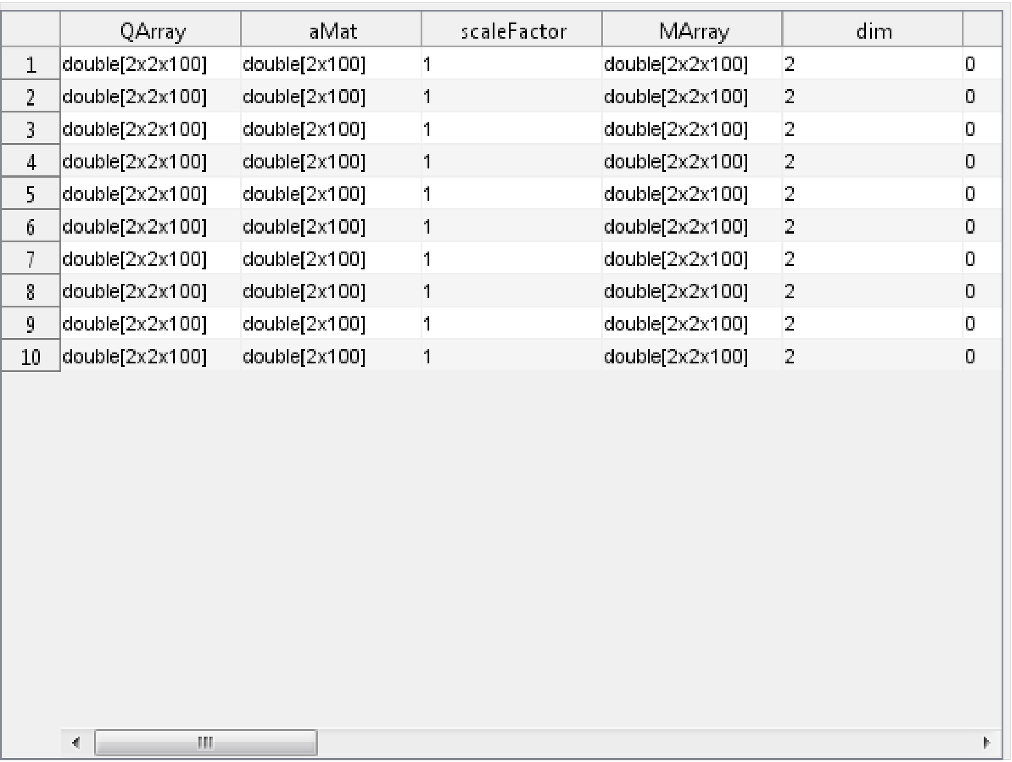
\includegraphics{dispPic.png}
\caption{Content of the ellipsoidal tube.}\label{chap_implement:disppic}\end{figure}

Figure \hyperref[chap_implement:dispPic]{ \ref*{chap_implement:dispPic}}
displays all fields of the ellipsoidal tube.

There are several methods to find the tubes with necessary parameters.

\begin{Verbatim}[commandchars=\\\{\},numbers=left,firstnumber=1,stepnumber=1]
\PYG{n}{newEllTube} \PYG{o}{=} \PYG{n}{fromMatEllTube}\PYG{p}{.}\PYG{n}{getTuplesFilteredBy}\PYG{p}{(}\PYG{err}{\PYGZsq{}}\PYG{n}{sTime}\PYG{err}{\PYGZsq{}}\PYG{p}{,} \PYG{l+m+mi}{5}\PYG{p}{)}\PYG{p}{;}
\PYG{n}{newEllTube}\PYG{p}{.}\PYG{n}{getNTuples}\PYG{p}{(}\PYG{p}{)}
\PYG{o}{\PYGZpc{}}
\PYG{o}{\PYGZpc{}} \PYG{n}{ans} \PYG{o}{=}
\PYG{o}{\PYGZpc{}} 
\PYG{o}{\PYGZpc{}}      \PYG{l+m+mi}{1}
\PYG{o}{\PYGZpc{}} 
\PYG{n}{newEllTube} \PYG{o}{=} \PYG{n}{fromMatEllTube}\PYG{p}{.}\PYG{n}{getTuplesFilteredBy}\PYG{p}{(}\PYG{err}{\PYGZsq{}}\PYG{n}{sTime}\PYG{err}{\PYGZsq{}}\PYG{p}{,} \PYG{l+m+mi}{2}\PYG{p}{)}\PYG{p}{;}
\PYG{n}{newEllTube}\PYG{p}{.}\PYG{n}{getNTuples}\PYG{p}{(}\PYG{p}{)}
\PYG{o}{\PYGZpc{}}
\PYG{o}{\PYGZpc{}} \PYG{n}{ans} \PYG{o}{=}
\PYG{o}{\PYGZpc{}} 
\PYG{o}{\PYGZpc{}}      \PYG{l+m+mi}{0}
\PYG{o}{\PYGZpc{}}
\end{Verbatim}

Also you can use the method display to see the result of the method’s
work.

\begin{Verbatim}[commandchars=\\\{\},numbers=left,firstnumber=1,stepnumber=1]
\PYG{n}{fromMatEllTube}\PYG{p}{.}\PYG{n}{getNTuples}\PYG{p}{(}\PYG{p}{)}
\PYG{o}{\PYGZpc{}}
\PYG{o}{\PYGZpc{}} \PYG{n}{ans} \PYG{o}{=}
\PYG{o}{\PYGZpc{}} 
\PYG{o}{\PYGZpc{}}      \PYG{l+m+mi}{1}
\PYG{o}{\PYGZpc{}} 
\PYG{n}{fromEllArrayEllTube}\PYG{p}{.}\PYG{n}{getNTuples}\PYG{p}{(}\PYG{p}{)}
\PYG{o}{\PYGZpc{}}
\PYG{o}{\PYGZpc{}} \PYG{n}{ans} \PYG{o}{=}
\PYG{o}{\PYGZpc{}} 
\PYG{o}{\PYGZpc{}}      \PYG{l+m+mi}{1}
\PYG{o}{\PYGZpc{}} 
\PYG{n}{origFromMatEllTube}\PYG{o}{=}\PYG{n}{fromMatEllTube}\PYG{p}{.}\PYG{n}{getCopy}\PYG{p}{(}\PYG{p}{)}\PYG{p}{;}
\PYG{n}{fromMatEllTube}\PYG{p}{.}\PYG{n}{unionWith}\PYG{p}{(}\PYG{n}{fromEllArrayEllTube}\PYG{p}{)}\PYG{p}{;}
\PYG{o}{\PYGZpc{}}
\PYG{o}{\PYGZpc{}} \PYG{n}{ans} \PYG{o}{=}
\PYG{o}{\PYGZpc{}} 
\PYG{o}{\PYGZpc{}}      \PYG{l+m+mi}{2}
\PYG{o}{\PYGZpc{}} 
\PYG{n}{fromMatEllTube}\PYG{p}{.}\PYG{n}{getNTuples}\PYG{p}{(}\PYG{p}{)}
\PYG{n}{isOk}\PYG{o}{=}\PYG{n}{fromMatEllTube}\PYG{p}{.}\PYG{n}{getTuples}\PYG{p}{(}\PYG{l+m+mi}{1}\PYG{p}{)}\PYG{p}{.}\PYG{n}{isEqual}\PYG{p}{(}\PYG{n}{origFromMatEllTube}\PYG{p}{)}
\PYG{o}{\PYGZpc{}}
\PYG{o}{\PYGZpc{}} \PYG{n}{isOk} \PYG{o}{=}
\PYG{o}{\PYGZpc{}}
\PYG{o}{\PYGZpc{}}     \PYG{l+m+mi}{1}

\PYG{n}{isOk}\PYG{o}{=}\PYG{n}{fromMatEllTube}\PYG{p}{.}\PYG{n}{getTuples}\PYG{p}{(}\PYG{l+m+mi}{2}\PYG{p}{)}\PYG{p}{.}\PYG{n}{isEqual}\PYG{p}{(}\PYG{n}{fromEllArrayEllTube}\PYG{p}{)}

\PYG{o}{\PYGZpc{}}
\PYG{o}{\PYGZpc{}} \PYG{n}{isOk} \PYG{o}{=}
\PYG{o}{\PYGZpc{}}
\PYG{o}{\PYGZpc{}}     \PYG{l+m+mi}{1}
\end{Verbatim}

We can sort our tubes by certain fields:

\begin{Verbatim}[commandchars=\\\{\},numbers=left,firstnumber=1,stepnumber=1]
\PYG{n}{fromMatEllTube}\PYG{p}{.}\PYG{n}{display}\PYG{p}{(}\PYG{p}{)}\PYG{p}{;}
\PYG{n}{fromMatEllTube}\PYG{p}{.}\PYG{n}{sortBy}\PYG{p}{(}\PYG{err}{\PYGZsq{}}\PYG{n}{sTime}\PYG{err}{\PYGZsq{}}\PYG{p}{)}\PYG{p}{;}
\PYG{n}{fromMatEllTube}\PYG{p}{.}\PYG{n}{display}\PYG{p}{(}\PYG{p}{)}\PYG{p}{;}
\end{Verbatim}


\section{Reachability}
\label{chap_implement:reachability}
To compute the reach sets of the systems described in chapter 3, we
define few new classes in the \emph{Ellipsoidal Toolbox}: class
LinSysContinuous for the continuous-time system description, class
LinSysDiscrete for the discrete-time system description and classes
ReachContinuous$\backslash$ReachDiscrete for the reach set
data. We start by explaining how to define a system using
LinSysContinuous object. Also we can use LinSysFactory class for the
description of this system. Through it’s method create user can get
LinSysContinuous or LinSysDiscrete object. For example, description of
the system
\begin{gather}
\begin{split}\left[\begin{array}{cc}
\dot{x}_1\\
\dot{x}_2\end{array}\right] = \left[\begin{array}{cc}
0 & 1\\
0 & 0\end{array}\right]\left[\begin{array}{c}
x_1\\
x_2\end{array}\right] + \left[\begin{array}{c}
u_1(t)\\
u_2(t)\end{array}\right], ~~~ u(t)\in{\mathcal E}(p(t), P)\end{split}\notag
\end{gather}
with
\begin{gather}
\begin{split}p(t) = \left[\begin{array}{c}
\sin(t)\\
\cos(t)\end{array}\right], ~~~ P = \left[\begin{array}{cc}
9 & 0\\
0 & 2\end{array}\right],\end{split}\notag
\end{gather}
is done by the following sequence of commands:

\begin{Verbatim}[commandchars=\\\{\},numbers=left,firstnumber=1,stepnumber=1]
\PYG{n}{aMat} \PYG{o}{=} \PYG{p}{[}\PYG{l+m+mi}{0} \PYG{l+m+mi}{1}\PYG{p}{;} \PYG{l+m+mi}{0} \PYG{l+m+mi}{0}\PYG{p}{]}\PYG{p}{;} \PYG{n}{bMat} \PYG{o}{=} \PYG{n}{eye}\PYG{p}{(}\PYG{l+m+mi}{2}\PYG{p}{)}\PYG{p}{;}  \PYG{o}{\PYGZpc{}} \PYG{n}{matrices} \PYG{n}{A} \PYG{n}{and} \PYG{n}{B}\PYG{p}{,} \PYG{n}{B} \PYG{n}{is} \PYG{n}{identity}
\PYG{n}{SUBounds} \PYG{o}{=} \PYG{k}{struct}\PYG{p}{(}\PYG{p}{)}\PYG{p}{;}
\PYG{o}{\PYGZpc{}} \PYG{n}{center} \PYG{n}{of} \PYG{n}{the} \PYG{n}{ellipsoid} \PYG{n}{depends} \PYG{n}{on} \PYG{n}{t}
\PYG{n}{SUBounds}\PYG{p}{.}\PYG{n}{center} \PYG{o}{=} \PYG{p}{\PYGZob{}}\PYG{err}{\PYGZsq{}}\PYG{n}{sin}\PYG{p}{(}\PYG{n}{t}\PYG{p}{)}\PYG{err}{\PYGZsq{}}\PYG{p}{;} \PYG{err}{\PYGZsq{}}\PYG{n}{cos}\PYG{p}{(}\PYG{n}{t}\PYG{p}{)}\PYG{err}{\PYGZsq{}}\PYG{p}{\PYGZcb{}}\PYG{p}{;}  
\PYG{n}{SUBounds}\PYG{p}{.}\PYG{n}{shape} \PYG{o}{=} \PYG{p}{[}\PYG{l+m+mi}{9} \PYG{l+m+mi}{0}\PYG{p}{;} \PYG{l+m+mi}{0} \PYG{l+m+mi}{2}\PYG{p}{]}\PYG{p}{;} \PYG{o}{\PYGZpc{}} \PYG{n}{shape} \PYG{n}{matrix} \PYG{n}{of} \PYG{n}{the} \PYG{n}{ellipsoid} \PYG{n}{is} \PYG{k}{static}
\PYG{o}{\PYGZpc{}} \PYG{n}{create} \PYG{n}{linear} \PYG{n}{system} \PYG{n}{object}
\PYG{n}{sys} \PYG{o}{=} \PYG{n}{elltool}\PYG{p}{.}\PYG{n}{linsys}\PYG{p}{.}\PYG{n}{LinSysContinuous}\PYG{p}{(}\PYG{n}{aMat}\PYG{p}{,} \PYG{n}{bMat}\PYG{p}{,} \PYG{n}{SUBounds}\PYG{p}{)}\PYG{p}{;} 
\PYG{o}{\PYGZpc{}} \PYG{n}{is} \PYG{n}{equal} \PYG{n}{to} \PYG{n}{sys} \PYG{o}{=} \PYG{n}{elltool}\PYG{p}{.}\PYG{n}{linsys}\PYG{p}{.}\PYG{n}{LinSysFactory}\PYG{p}{.}\PYG{n}{create}\PYG{p}{(}\PYG{n}{aMat}\PYG{p}{,} \PYG{n}{bMat}\PYG{p}{,} \PYG{n}{SUBounds}\PYG{p}{)}
\end{Verbatim}

If matrices $A$ or
$B$ depend on time, say $A(t)=\left[\begin{array}{cc}
0 & 1-\cos(2t)\\
-\frac{1}{t} & 0\end{array}\right]$, then matrix aMat should be
symbolic:

\begin{Verbatim}[commandchars=\\\{\},numbers=left,firstnumber=1,stepnumber=1]
\PYG{n}{atMat} \PYG{o}{=} \PYG{p}{\PYGZob{}}\PYG{l+s+sc}{\PYGZsq{}0\PYGZsq{}} \PYG{err}{\PYGZsq{}}\PYG{l+m+mi}{1} \PYG{o}{\PYGZhy{}} \PYG{n}{cos}\PYG{p}{(}\PYG{l+m+mi}{2}\PYG{o}{*}\PYG{n}{t}\PYG{p}{)}\PYG{err}{\PYGZsq{}}\PYG{p}{;} \PYG{err}{\PYGZsq{}}\PYG{o}{\PYGZhy{}}\PYG{l+m+mi}{1}\PYG{o}{/}\PYG{n}{t}\PYG{l+s+sc}{\PYGZsq{} \PYGZsq{}}\PYG{l+m+mi}{0}\PYG{err}{\PYGZsq{}}\PYG{p}{\PYGZcb{}}\PYG{p}{;}  
\PYG{k+kt}{sys\PYGZus{}t} \PYG{o}{=} \PYG{n}{elltool}\PYG{p}{.}\PYG{n}{linsys}\PYG{p}{.}\PYG{n}{LinSysFactory}\PYG{p}{.}\PYG{n}{create}\PYG{p}{(}\PYG{n}{atMat}\PYG{p}{,} \PYG{n}{bMat}\PYG{p}{,} \PYG{n}{SUBounds}\PYG{p}{)}\PYG{p}{;}
\end{Verbatim}

To describe the system with disturbance
\begin{gather}
\begin{split}\left[\begin{array}{cc}
\dot{x}_1\\
\dot{x}_2\end{array}\right] = \left[\begin{array}{cc}
0 & 1\\
0 & 0\end{array}\right]\left[\begin{array}{c}
x_1\\
x_2\end{array}\right] + \left[\begin{array}{c}
u_1(t)\\
u_2(t)\end{array}\right] + \left[\begin{array}{c}
0\\
1\end{array}\right]v(t),\end{split}\notag
\end{gather}
with bounds on control as before, and disturbance being
$-1\leqslant v(t)\leqslant1$, we type:

\begin{Verbatim}[commandchars=\\\{\},numbers=left,firstnumber=1,stepnumber=1]
\PYG{n}{gMat} \PYG{o}{=} \PYG{p}{[}\PYG{l+m+mi}{0}\PYG{p}{;} \PYG{l+m+mi}{1}\PYG{p}{]}\PYG{p}{;}  \PYG{o}{\PYGZpc{}} \PYG{n}{matrix} \PYG{n}{G}
\PYG{n}{vEllObj} \PYG{o}{=} \PYG{n}{ellipsoid}\PYG{p}{(}\PYG{l+m+mi}{1}\PYG{p}{)}\PYG{p}{;}  \PYG{o}{\PYGZpc{}} \PYG{n}{disturbance} \PYG{n}{bounds}\PYG{o}{:} \PYG{n}{unit} \PYG{n}{ball} \PYG{n}{in} \PYG{n}{R}
\PYG{n}{sys\PYGZus{}d} \PYG{o}{=} \PYG{n}{elltool}\PYG{p}{.}\PYG{n}{linsys}\PYG{p}{.}\PYG{n}{LinSysContinuous}\PYG{p}{(}\PYG{n}{aMat}\PYG{p}{,} \PYG{n}{bMat}\PYG{p}{,} \PYG{n}{SUBounds}\PYG{p}{,}\PYG{p}{.}\PYG{p}{.}\PYG{p}{.}
    \PYG{n}{gMat}\PYG{p}{,} \PYG{n}{vEllObj}\PYG{p}{)}\PYG{p}{;}
\end{Verbatim}

Control and disturbance
bounds SUBounds and vEllObj can have different types. If the bound is
constant, it should be described by ellipsoid object. If the bound
depends on time, then it is represented by a structure with fields
center and shape, one or both of which are symbolic. In system sys, the
control bound SUBounds is defined as such a structure. Finally, if the
control or disturbance is known and fixed, it should be defined as a
vector, of type double if constant, or symbolic, if it depends on time.

To declare a discrete-time system
\begin{gather}
\begin{split}\left[\begin{array}{c}
x_1[k+1]\\
x_2[k+1]\end{array}\right] = \left[\begin{array}{cc}
0 & 1\\
-1 & -0.5\end{array}\right]\left[\begin{array}{c}
x_1[k]\\
x_2[k]\end{array}\right] + \left[\begin{array}{c}
0\\
1\end{array}\right]u[k], ~~~ -1\leqslant u[k]\leqslant1,\end{split}\notag
\end{gather}
we use LinSysDiscrete constructor:

\begin{Verbatim}[commandchars=\\\{\},numbers=left,firstnumber=1,stepnumber=1]
\PYG{n}{adMat} \PYG{o}{=} \PYG{p}{[}\PYG{l+m+mi}{0} \PYG{l+m+mi}{1}\PYG{p}{;} \PYG{o}{\PYGZhy{}}\PYG{l+m+mi}{1} \PYG{o}{\PYGZhy{}}\PYG{l+m+mf}{0.5}\PYG{p}{]}\PYG{p}{;} \PYG{n}{bdMat} \PYG{o}{=} \PYG{p}{[}\PYG{l+m+mi}{0}\PYG{p}{;} \PYG{l+m+mi}{1}\PYG{p}{]}\PYG{p}{;}  \PYG{o}{\PYGZpc{}} \PYG{n}{matrices} \PYG{n}{A} \PYG{n}{and} \PYG{n}{B}
\PYG{n}{udBoundsEllObj}  \PYG{o}{=} \PYG{n}{ellipsoid}\PYG{p}{(}\PYG{l+m+mi}{1}\PYG{p}{)}\PYG{p}{;}  \PYG{o}{\PYGZpc{}} \PYG{n}{control} \PYG{n}{bounds}\PYG{o}{:} \PYG{n}{unit} \PYG{n}{ball} \PYG{n}{in} \PYG{n}{R}
\PYG{o}{\PYGZpc{}} \PYG{n}{discrete}\PYG{o}{\PYGZhy{}}\PYG{n}{time} \PYG{n}{system}
\PYG{n}{dtsys} \PYG{o}{=} \PYG{n}{elltool}\PYG{p}{.}\PYG{n}{linsys}\PYG{p}{.}\PYG{n}{LinSysDiscrete}\PYG{p}{(}\PYG{n}{adMat}\PYG{p}{,} \PYG{n}{bdMat}\PYG{p}{,} \PYG{n}{udBoundsEllObj}\PYG{p}{)}\PYG{p}{;} 
\PYG{o}{\PYGZpc{}} \PYG{n}{is} \PYG{n}{equal} \PYG{n}{to} \PYG{n}{dtsys} \PYG{o}{=} \PYG{n}{elltool}\PYG{p}{.}\PYG{n}{linsys}\PYG{p}{.}\PYG{n}{LinSysFactory}\PYG{p}{.}\PYG{n}{create}\PYG{p}{(}\PYG{n}{adMat}\PYG{p}{,} \PYG{n}{bdMat}\PYG{p}{,}\PYG{p}{.}\PYG{p}{.}\PYG{p}{.}
\PYG{o}{\PYGZpc{}}         \PYG{n}{udBoundsEllObj}\PYG{p}{,}\PYG{p}{.}\PYG{p}{.}\PYG{p}{.}\PYG{p}{[}\PYG{p}{]}\PYG{p}{,} \PYG{p}{[}\PYG{p}{]}\PYG{p}{,} \PYG{p}{[}\PYG{p}{]}\PYG{p}{,} \PYG{p}{[}\PYG{p}{]}\PYG{p}{,} \PYG{l+s+sc}{\PYGZsq{}d\PYGZsq{}}\PYG{p}{)}\PYG{p}{;}
\end{Verbatim}

Once the LinSysDiscrete object is
created, we need to specify the set of initial conditions, the time
interval and values of the direction vector, for which the reach set
approximations must be computed:

\begin{Verbatim}[commandchars=\\\{\},numbers=left,firstnumber=1,stepnumber=1]
\PYG{n}{x0EllObj} \PYG{o}{=} \PYG{n}{ell\PYGZus{}unitball}\PYG{p}{(}\PYG{l+m+mi}{2}\PYG{p}{)}\PYG{p}{;}  \PYG{o}{\PYGZpc{}} \PYG{n}{set} \PYG{n}{of} \PYG{n}{initial} \PYG{n}{conditions}
\PYG{n}{timeVec} \PYG{o}{=} \PYG{p}{[}\PYG{l+m+mi}{0} \PYG{l+m+mi}{10}\PYG{p}{]}\PYG{p}{;}  \PYG{o}{\PYGZpc{}} \PYG{n}{time} \PYG{n}{interval}
\PYG{n}{dirsMat} \PYG{o}{=} \PYG{p}{[}\PYG{l+m+mi}{1} \PYG{l+m+mi}{0}\PYG{p}{;} \PYG{l+m+mi}{0} \PYG{l+m+mi}{1}\PYG{p}{]}\PYG{err}{\PYGZsq{}}\PYG{p}{;}  \PYG{o}{\PYGZpc{}} \PYG{n}{columns} \PYG{n}{of} \PYG{n}{L} \PYG{n}{specify} \PYG{n}{the} \PYG{n}{directions}
\end{Verbatim}

The reach set approximation is computed
by calling the constructor of the ReachContinuous object:

\begin{Verbatim}[commandchars=\\\{\},numbers=left,firstnumber=1,stepnumber=1]
\PYG{c}{\PYGZpc{} reach set of continuos\PYGZhy{}time system}
\PYG{n}{firstRsObj} \PYG{p}{=} \PYG{n}{elltool}\PYG{p}{.}\PYG{n}{reach}\PYG{p}{.}\PYG{n}{ReachContinuous}\PYG{p}{(}\PYG{n}{sys}\PYG{p}{,} \PYG{n}{x0EllObj}\PYG{p}{,} \PYG{n}{dirsMat}\PYG{p}{,} \PYG{n}{timeVec}\PYG{p}{)}\PYG{p}{;}
\end{Verbatim}

At this point,
variable firstRsObj contains the reach set approximations for the
specified continuous-time system, time interval and set of initial
conditions computed for given directions. Both external and internal
approximations are computed. The reach set approximation data can be
extracted in the form of arrays of ellipsoids:

\begin{Verbatim}[commandchars=\\\{\},numbers=left,firstnumber=1,stepnumber=1]
\PYG{n}{externallEllMat} \PYG{o}{=} \PYG{n}{firstRsObj}\PYG{p}{.}\PYG{n}{get\PYGZus{}ea}\PYG{p}{(}\PYG{p}{)}  \PYG{o}{\PYGZpc{}} \PYG{n}{external} \PYG{n}{approximating} \PYG{n}{ellipsoids}

\PYG{o}{\PYGZpc{}} \PYG{n}{externallEllMat} \PYG{o}{=}
\PYG{o}{\PYGZpc{}} \PYG{n}{Array} \PYG{n}{of} \PYG{n}{ellipsoids} \PYG{n}{with} \PYG{n}{dimensionality} \PYG{l+m+mi}{2}\PYG{n}{x100}

\PYG{o}{\PYGZpc{}} \PYG{n}{internal} \PYG{n}{approximating} \PYG{n}{ellipsoids}
\PYG{p}{[}\PYG{n}{internalEllMat}\PYG{p}{,} \PYG{n}{timeVec}\PYG{p}{]} \PYG{o}{=} \PYG{n}{firstRsObj}\PYG{p}{.}\PYG{n}{get\PYGZus{}ia}\PYG{p}{(}\PYG{p}{)}\PYG{p}{;}
\end{Verbatim}

Ellipsoidal arrays externallEllMat and internalEllMat have $4$
rows because we computed the reach set approximations for $4$
directions. Each row of ellipsoids corresponds to one direction. The
number of columns in externallEllMat and internalEllMat is defined by
the nTimeGridPoints parameter, which is available from
elltool.conf.Properties static class (see chapter 6 for details). It
represents the number of time values in our time interval, at which the
approximations are evaluated. These time values are returned in the
optinal output parameter, array timeVec, whose length is the same as the
number of columns in externallEllMat and internalEllMat. Intersection of
ellipsoids in a particular column of externallEllMat gives external
ellipsoidal approximation of the reach set at corresponding time.
Internal ellipsoidal approximation of this set at this time is given by
the union of ellipsoids in the same column of internalEllMat.

We may be interested in the reachability data of our system in some
particular time interval, smaller than the one for which the reach set
was computed, say $3\leqslant t\leqslant5$. This data can be
extracted and returned in the form of ReachContinuous object by the cut
function:

\begin{Verbatim}[commandchars=\\\{\},numbers=left,firstnumber=1,stepnumber=1]
\PYG{n}{cutObj} \PYG{o}{=} \PYG{n}{firstRsObj}\PYG{p}{.}\PYG{n}{cut}\PYG{p}{(}\PYG{p}{[}\PYG{l+m+mi}{3} \PYG{l+m+mi}{5}\PYG{p}{]}\PYG{p}{)}\PYG{p}{;}  \PYG{o}{\PYGZpc{}} \PYG{n}{reach} \PYG{n}{set} \PYG{k}{for} \PYG{n}{the} \PYG{n}{time} \PYG{n}{interval} \PYG{p}{[}\PYG{l+m+mi}{3}\PYG{p}{,} \PYG{l+m+mi}{5}\PYG{p}{]}
\end{Verbatim}

To obtain a snap shot of the reach set at given time, the same function
cut is used:

\begin{Verbatim}[commandchars=\\\{\},numbers=left,firstnumber=1,stepnumber=1]
\PYG{n}{cutObj} \PYG{o}{=} \PYG{n}{firstRsObj}\PYG{p}{.}\PYG{n}{cut}\PYG{p}{(}\PYG{l+m+mi}{5}\PYG{p}{)}\PYG{p}{;}  \PYG{o}{\PYGZpc{}} \PYG{n}{reach} \PYG{n}{set} \PYG{n}{at} \PYG{n}{time} \PYG{n}{t} \PYG{o}{=} \PYG{l+m+mi}{5}
\end{Verbatim}

It can be checked if the external or internal reach set
approximation intersects with given ellipsoids, hyperplanes or
polytopes:

\begin{Verbatim}[commandchars=\\\{\},numbers=left,firstnumber=1,stepnumber=1]
\PYG{n}{ellObj} \PYG{o}{=} \PYG{n}{ellipsoid}\PYG{p}{(}\PYG{p}{[}\PYG{o}{\PYGZhy{}}\PYG{l+m+mi}{17}\PYG{p}{;} \PYG{l+m+mi}{0}\PYG{p}{]}\PYG{p}{,} \PYG{p}{[}\PYG{l+m+mi}{4} \PYG{o}{\PYGZhy{}}\PYG{l+m+mi}{1}\PYG{p}{;} \PYG{o}{\PYGZhy{}}\PYG{l+m+mi}{1} \PYG{l+m+mi}{1}\PYG{p}{]}\PYG{p}{)}\PYG{p}{;}  \PYG{o}{\PYGZpc{}} \PYG{n}{define} \PYG{n}{ellipsoid}
\PYG{o}{\PYGZpc{}} \PYG{n}{define} \PYG{l+m+mi}{4} \PYG{n}{hyperplanes}
\PYG{n}{hypVec} \PYG{o}{=} \PYG{n}{hyperplane}\PYG{p}{(}\PYG{p}{[}\PYG{l+m+mi}{1} \PYG{l+m+mi}{1}\PYG{p}{;} \PYG{o}{\PYGZhy{}}\PYG{l+m+mi}{1} \PYG{o}{\PYGZhy{}}\PYG{l+m+mi}{1}\PYG{p}{;} \PYG{l+m+mi}{1} \PYG{o}{\PYGZhy{}}\PYG{l+m+mi}{1}\PYG{p}{;} \PYG{o}{\PYGZhy{}}\PYG{l+m+mi}{1} \PYG{l+m+mi}{1}\PYG{p}{]}\PYG{err}{\PYGZsq{}}\PYG{p}{,} \PYG{p}{[}\PYG{l+m+mi}{2} \PYG{l+m+mi}{2} \PYG{l+m+mi}{2} \PYG{l+m+mi}{2}\PYG{p}{]}\PYG{p}{)}\PYG{p}{;} 
\PYG{n}{polObj} \PYG{o}{=} \PYG{n}{hyperplane2polytope}\PYG{p}{(}\PYG{n}{hypVec}\PYG{p}{)} \PYG{o}{+} \PYG{p}{[}\PYG{l+m+mi}{2}\PYG{p}{;} \PYG{l+m+mi}{10}\PYG{p}{]}\PYG{p}{;}  \PYG{o}{\PYGZpc{}} \PYG{n}{define} \PYG{n}{polytope}
\PYG{o}{\PYGZpc{}} \PYG{n}{check} \PYG{k}{if} \PYG{n}{ellipsoid} \PYG{n}{ell} \PYG{n}{intersects} \PYG{n}{with} \PYG{n}{external} \PYG{n}{approximation}\PYG{o}{:}
\PYG{n}{cutObj}\PYG{p}{.}\PYG{n}{intersect}\PYG{p}{(}\PYG{n}{ellObj}\PYG{p}{,} \PYG{l+s+sc}{\PYGZsq{}e\PYGZsq{}}\PYG{p}{)}

\PYG{o}{\PYGZpc{}} \PYG{n}{ans} \PYG{o}{=}
\PYG{o}{\PYGZpc{}} 
\PYG{o}{\PYGZpc{}}      \PYG{l+m+mi}{1}
\end{Verbatim}

\begin{Verbatim}[commandchars=\\\{\},numbers=left,firstnumber=1,stepnumber=1]
\PYG{c}{\PYGZpc{} check if ellipsoid ellObj intersects with internal approximation:}
\PYG{n}{cutObj}\PYG{p}{.}\PYG{n}{intersect}\PYG{p}{(}\PYG{n}{ellObj}\PYG{p}{,} \PYG{l+s}{\PYGZsq{}}\PYG{l+s}{i\PYGZsq{}}\PYG{p}{)}

\PYG{c}{\PYGZpc{} }
\PYG{c}{\PYGZpc{} ans =}
\PYG{c}{\PYGZpc{} }
\PYG{c}{\PYGZpc{}      1}
\end{Verbatim}

\begin{Verbatim}[commandchars=\\\{\},numbers=left,firstnumber=1,stepnumber=1]
\PYG{c}{\PYGZpc{} check if hyperplanes in hypVec intersect with internal approximation:}
\PYG{n}{cutObj}\PYG{p}{.}\PYG{n}{intersect}\PYG{p}{(}\PYG{n}{hypVec}\PYG{p}{,} \PYG{l+s}{\PYGZsq{}}\PYG{l+s}{i\PYGZsq{}}\PYG{p}{)}

\PYG{c}{\PYGZpc{} ans =}
\PYG{c}{\PYGZpc{} }
\PYG{c}{\PYGZpc{}      1     1     1     1}
\end{Verbatim}

\begin{Verbatim}[commandchars=\\\{\},numbers=left,firstnumber=1,stepnumber=1]
\PYG{c}{\PYGZpc{} check if polytope polObj intersects with external approximation:}
\PYG{n}{cutObj}\PYG{p}{.}\PYG{n}{intersect}\PYG{p}{(}\PYG{n}{polObj}\PYG{p}{)}

\PYG{c}{\PYGZpc{} ans =}
\PYG{c}{\PYGZpc{} }
\PYG{c}{\PYGZpc{}      0}
\end{Verbatim}

If a given set intersects with the internal approximation of the reach
set, then this set intersects with the actual reach set. If the given
set does not intersect with external approximation, this set does not
intersect the actual reach set. There are situations, however, when the
given set intersects with the external approximation but does not
intersect with the internal one. In our example above, ellipsoid ellObj
is such a case: the quality of the approximation does not allow us to
determine whether or not ellObj intersects with the actual reach set. To
improve the quality of approximation, refine function should be used:

\begin{Verbatim}[commandchars=\\\{\},numbers=left,firstnumber=1,stepnumber=1]
\PYG{c}{\PYGZpc{} define new directions, in this case one, but could be more}
\PYG{n}{newDirsMat} \PYG{p}{=} \PYG{p}{[}\PYG{l+m+mi}{1}\PYG{p}{;} \PYG{o}{\PYGZhy{}}\PYG{l+m+mi}{1}\PYG{p}{]}\PYG{p}{;}
\PYG{c}{\PYGZpc{} compute approximations for the new directions}
\PYG{n}{firstRsObj} \PYG{p}{=} \PYG{n}{firstRsObj}\PYG{p}{.}\PYG{n}{refine}\PYG{p}{(}\PYG{n}{newDirsMat}\PYG{p}{)}\PYG{p}{;}
\PYG{c}{\PYGZpc{} snap shot of the reach set at time t = 5}
\PYG{n}{cutObj} \PYG{p}{=} \PYG{n}{firstRsObj}\PYG{p}{.}\PYG{n}{cut}\PYG{p}{(}\PYG{l+m+mi}{5}\PYG{p}{)}\PYG{p}{;}
\PYG{c}{\PYGZpc{} check if ellObj intersects the internal approximation}
\PYG{n}{cutObj}\PYG{p}{.}\PYG{n}{intersect}\PYG{p}{(}\PYG{n}{ellObj}\PYG{p}{,} \PYG{l+s}{\PYGZsq{}}\PYG{l+s}{i\PYGZsq{}}\PYG{p}{)}  

\PYG{c}{\PYGZpc{} ans =}
\PYG{c}{\PYGZpc{} }
\PYG{c}{\PYGZpc{}      1}
\end{Verbatim}

Now we are sure that ellipsoid ellObj intersects with the actual reach
set. However, to use the refine function, the reach set object must
contain all calculated data, otherwise, an error is returned.

Having a reach set object resulting from the ReachContinuous, cut or
refine operations, we can obtain the trajectory of the center of the
reach set and the good curves along which the actual reach set is
touched by its ellipsoidal approximations:

\begin{Verbatim}[commandchars=\\\{\},numbers=left,firstnumber=1,stepnumber=1]
\PYG{p}{[}\PYG{n}{ctrMat}\PYG{p}{,} \PYG{n}{ttVec}\PYG{p}{]} \PYG{o}{=} \PYG{n}{firstRsObj}\PYG{p}{.}\PYG{n}{get\PYGZus{}center}\PYG{p}{(}\PYG{p}{)}\PYG{p}{;} \PYG{o}{\PYGZpc{}} \PYG{n}{trajectory} \PYG{n}{of} \PYG{n}{the} \PYG{n}{center}
\PYG{n}{gcCVec} \PYG{o}{=} \PYG{n}{firstRsObj}\PYG{p}{.}\PYG{n}{get\PYGZus{}goodcurves}\PYG{p}{(}\PYG{p}{)}  \PYG{o}{\PYGZpc{}} \PYG{n}{get} \PYG{n}{good} \PYG{n}{curves}

\PYG{o}{\PYGZpc{}} \PYG{n}{gcCVec} \PYG{o}{=}
\PYG{o}{\PYGZpc{}} \PYG{p}{[}\PYG{l+m+mi}{2}\PYG{n}{x100} \PYG{k+kt}{double}\PYG{p}{]} \PYG{p}{[}\PYG{l+m+mi}{2}\PYG{n}{x100} \PYG{k+kt}{double}\PYG{p}{]} \PYG{p}{[}\PYG{l+m+mi}{2}\PYG{n}{x100} \PYG{k+kt}{double}\PYG{p}{]}
\end{Verbatim}

Variable ctrMat here is a matrix whose columns are the points ofthe
reach set center trajectory evaluated at time values returned in the
array ttVec. Variable gcCMat contains $4$ matrices each of which
corresponds to a good curve (columns of such matrix are points of the
good curve evaluated at time values in ttVec). The analytic expression
for the control driving the system along a good curve is given by
formula \eqref{chap_implement-uct}.

We computed the reach set up to time $10$. It is possible to
continue the reach set computation for a longer time horizon using the
reach set data at time $10$ as initial condition. It is also
possible that the dynamics and inputs of the system change at certain
time, and from that point on the system evolves according to the new
system of differential equations. For example, starting at time
$10$, our reach set may evolve in time according to the
time-variant system sys\_t defined above. Switched systems are a special
case of this situation. To compute the further evolution in time of the
existing reach set, function evolve should be used:

\begin{Verbatim}[commandchars=\\\{\},numbers=left,firstnumber=1,stepnumber=1]
\PYG{c}{\PYGZpc{} reach set from time 10 to 14 with the same dynamics}
\PYG{n}{secRsObj} \PYG{p}{=} \PYG{n}{firstRsObj}\PYG{p}{.}\PYG{n}{evolve}\PYG{p}{(}\PYG{l+m+mi}{14}\PYG{p}{)}\PYG{p}{;} 
\PYG{c}{\PYGZpc{} reach set from time 10 to 12 with new dynamics}
\PYG{n}{secRsObj} \PYG{p}{=} \PYG{n}{firstRsObj}\PYG{p}{.}\PYG{n}{evolve}\PYG{p}{(}\PYG{l+m+mi}{12}\PYG{p}{,} \PYG{n}{sys\PYGZus{}t}\PYG{p}{)}\PYG{p}{;}  

\PYG{c}{\PYGZpc{} not only the dynamics, but the inputs can change as well,}
\PYG{c}{\PYGZpc{} from time 12 to 13 disturbance is added to the system:}

\PYG{c}{\PYGZpc{} sys\PYGZus{}d \PYGZhy{} system with disturbance defined above}
\PYG{n}{thirdRsObj} \PYG{p}{=} \PYG{n}{secRsObj}\PYG{p}{.}\PYG{n}{evolve}\PYG{p}{(}\PYG{l+m+mi}{13}\PYG{p}{,} \PYG{n}{sys\PYGZus{}d}\PYG{p}{)}\PYG{p}{;}
\end{Verbatim}

Function evolve can
be viewed as an implementation of the semigroup property.

To compute the backward reach set for some specified target set, we
declare the time interval so that the terminating time comes first:

\begin{Verbatim}[commandchars=\\\{\},numbers=left,firstnumber=1,stepnumber=1]
\PYG{c}{\PYGZpc{} target set in the form of ellipsoid}
\PYG{n}{yEllObj} \PYG{p}{=} \PYG{n}{ellipsoid}\PYG{p}{(}\PYG{p}{[}\PYG{l+m+mi}{8}\PYG{p}{;} \PYG{l+m+mi}{2}\PYG{p}{]}\PYG{p}{,} \PYG{p}{[}\PYG{l+m+mi}{4} \PYG{l+m+mi}{1}\PYG{p}{;} \PYG{l+m+mi}{1} \PYG{l+m+mi}{2}\PYG{p}{]}\PYG{p}{)}\PYG{p}{;}
\PYG{n}{tbTimeVec} \PYG{p}{=} \PYG{p}{[}\PYG{l+m+mi}{10} \PYG{l+m+mi}{5}\PYG{p}{]}\PYG{p}{;}  \PYG{c}{\PYGZpc{} backward time interval}
\PYG{c}{\PYGZpc{} backward reach set}
\PYG{n}{firstBrsObj} \PYG{p}{=} \PYG{n}{elltool}\PYG{p}{.}\PYG{n}{reach}\PYG{p}{.}\PYG{n}{ReachContinuous}\PYG{p}{(}\PYG{n}{sys}\PYG{p}{,} \PYG{n}{yEllObj}\PYG{p}{,} \PYG{n}{dirsMat}\PYG{p}{,}\PYG{c}{...}
        \PYG{n}{tbTimeVec}\PYG{p}{)}\PYG{p}{;}  
\PYG{n}{firstBrsObj} \PYG{p}{=} \PYG{n}{firstBrsObj}\PYG{p}{.}\PYG{n}{refine}\PYG{p}{(}\PYG{n}{newDirsMat}\PYG{p}{)}\PYG{p}{;}  \PYG{c}{\PYGZpc{} refine the approximation}
\PYG{c}{\PYGZpc{} further evolution in backward time from 5 to 0; }
\PYG{n}{secBrsObj} \PYG{p}{=} \PYG{n}{firstBrsObj}\PYG{p}{.}\PYG{n}{evolve}\PYG{p}{(}\PYG{l+m+mi}{0}\PYG{p}{)}
\end{Verbatim}

Reach set and backward reach set computation for discrete-time systems
and manipulations with the resulting reach set object are performed
using the same functions as for continuous-time systems:

\begin{Verbatim}[commandchars=\\\{\},numbers=left,firstnumber=1,stepnumber=1]
\PYG{n}{timeVec} \PYG{o}{=} \PYG{p}{[}\PYG{l+m+mi}{0} \PYG{l+m+mi}{100}\PYG{p}{]}\PYG{p}{;}  \PYG{o}{\PYGZpc{}} \PYG{n}{represents} \PYG{l+m+mi}{100} \PYG{n}{time} \PYG{n}{steps} \PYG{n}{from} \PYG{l+m+mi}{1} \PYG{n}{to} \PYG{l+m+mi}{100}
\PYG{o}{\PYGZpc{}} \PYG{n}{reach} \PYG{n}{set} \PYG{k}{for} \PYG{l+m+mi}{100} \PYG{n}{time} \PYG{n}{steps}
\PYG{n}{secDtrsObj} \PYG{o}{=} \PYG{n}{elltool}\PYG{p}{.}\PYG{n}{reach}\PYG{p}{.}\PYG{n}{ReachDiscrete}\PYG{p}{(}\PYG{n}{dtsys}\PYG{p}{,} \PYG{n}{x0EllObj}\PYG{p}{,} \PYG{n}{dirsMat}\PYG{p}{,} \PYG{n}{timeVec}\PYG{p}{)}\PYG{p}{;} 
\PYG{n}{secDtrsObj} \PYG{o}{=} \PYG{n}{secDtrsObj}\PYG{p}{.}\PYG{n}{evolve}\PYG{p}{(}\PYG{l+m+mi}{200}\PYG{p}{)}\PYG{p}{;}  \PYG{o}{\PYGZpc{}} \PYG{n}{compute} \PYG{n}{next} \PYG{l+m+mi}{100} \PYG{n}{time} \PYG{n}{steps}

\PYG{n}{tbTimeVec} \PYG{o}{=} \PYG{p}{[}\PYG{l+m+mi}{50} \PYG{l+m+mi}{0}\PYG{p}{]}\PYG{p}{;}  \PYG{o}{\PYGZpc{}} \PYG{n}{backward} \PYG{n}{time} \PYG{n}{interval}
\PYG{o}{\PYGZpc{}} \PYG{n}{backward} \PYG{n}{reach} \PYG{n}{set}
\PYG{n}{dtbrsObj} \PYG{o}{=} \PYG{n}{elltool}\PYG{p}{.}\PYG{n}{reach}\PYG{p}{.}\PYG{n}{ReachDiscrete}\PYG{p}{(}\PYG{n}{dtsys}\PYG{p}{,} \PYG{n}{yEllObj}\PYG{p}{,} \PYG{n}{dirsMat}\PYG{p}{,} \PYG{n}{tbTimeVec}\PYG{p}{)}\PYG{p}{;}  
\PYG{n}{dtbrsObj} \PYG{o}{=} \PYG{n}{dtbrsObj}\PYG{p}{.}\PYG{n}{refine}\PYG{p}{(}\PYG{n}{newDirsMat}\PYG{p}{)}\PYG{p}{;}  \PYG{o}{\PYGZpc{}} \PYG{n}{refine} \PYG{n}{the} \PYG{n}{approximation}
\PYG{o}{\PYGZpc{}} \PYG{n}{get} \PYG{n}{external} \PYG{n}{approximating} \PYG{n}{ellipsoids} \PYG{n}{and} \PYG{n}{time} \PYG{n}{values}
\PYG{p}{[}\PYG{n}{externallEllMat}\PYG{p}{,} \PYG{n}{timeVec}\PYG{p}{]} \PYG{o}{=} \PYG{n}{dtbrsObj}\PYG{p}{.}\PYG{n}{get\PYGZus{}ea}\PYG{p}{(}\PYG{p}{)}\PYG{p}{;}
\PYG{o}{\PYGZpc{}} \PYG{n}{get} \PYG{n}{internal} \PYG{n}{approximating} \PYG{n}{ellipsoids}
\PYG{n}{internalEllMat} \PYG{o}{=} \PYG{n}{dtbrsObj}\PYG{p}{.}\PYG{n}{get\PYGZus{}ia}\PYG{p}{(}\PYG{p}{)}

\PYG{o}{\PYGZpc{}} \PYG{n}{internalEllMat} \PYG{o}{=}
\PYG{o}{\PYGZpc{}} \PYG{n}{Array} \PYG{n}{of} \PYG{n}{ellipsoids} \PYG{n}{with} \PYG{n}{dimensionality} \PYG{l+m+mi}{3}\PYG{n}{x51}
\end{Verbatim}

Number of columns in the ellipsoidal arrays externalEllMat and
internalEllMat is $51$ because the backward reach set is computed
for $50$ time steps, and the first column of these arrays contains
$3$ ellipsoids yEllObj - the terminating condition.

When dealing with discrete-time systems, all functions that accept time
or time interval as an input parameter, round the time values and treat
them as integers.


\section{Properties}
\label{chap_implement:properties}
Functions of the \emph{Ellipsoidal Toolbox} can be called with user-specified
values of certain global parameters. System of the parameters are
configured using xml files, which available from a set of command-line
utilities:

\begin{Verbatim}[commandchars=\\\{\},numbers=left,firstnumber=1,stepnumber=1]
\PYG{n}{elltool}\PYG{p}{.}\PYG{n}{setconf}\PYG{p}{(}\PYG{err}{\PYGZsq{}}\PYG{k}{default}\PYG{err}{\PYGZsq{}}\PYG{p}{)}\PYG{p}{;}
\end{Verbatim}

Here we list system parameters available from the ’default’
configuration:
\begin{enumerate}
\item {} 
version = ’1.4dev’ - current version of \emph{ET}.

\item {} 
isVerbose = false - makes all the calls to \emph{ET} routines silent, and
no information except errors is displayed.

\item {} 
absTol = 1e-7 - absolute tolerance.

\item {} 
relTol = 1e-5 - relative tolerance.

\item {} 
nTimeGridPoints = 200 - density of the time grid for the continuous
time reach set computation. This parameter directly affects the
number of ellipsoids to be stored in the
ReachContinuous$\backslash$ReachDiscrete object.

\item {} 
ODESolverName = ode45 - specifies the ODE solver for continuous time
reach set computation.

\item {} 
isODENormControl = ’on’ - switches on and off the norm control in the
ODE solver. When turned on, it slows down the computation, but
improves the accuracy.

\item {} 
isEnabledOdeSolverOptions = false - when set to false, calls the ODE
solver without any additional options like norm control. It makes the
computation faster but less accurate. Otherwise, it is assumed to be
true, and only in this case the previous option makes a difference.

\item {} 
nPlot2dPoints = 200 - the number of points used to plot a 2D
ellipsoid. This parameter also affects the quality of 2D reach tube
and reach set plots.

\item {} 
nPlot3dPoints = 200 - the number of points used to plot a 3D
ellipsoid. This parameter also affects the quality of 3D reach set
plots.

\end{enumerate}

Once the configuration is loaded, the system parameters are available
through elltool.conf.Properties. elltool.conf.Properties is a static
class, providing emulation of static properties for toolbox. It has two
function types: setters and getters. Using getters we obtain system
parameters.

\begin{Verbatim}[commandchars=\\\{\},numbers=left,firstnumber=1,stepnumber=1]
\PYG{n}{elltool}\PYG{p}{.}\PYG{n}{conf}\PYG{p}{.}\PYG{n}{Properties}\PYG{p}{.}\PYG{n}{getAbsTol}\PYG{p}{(}\PYG{p}{)}
\PYG{o}{\PYGZpc{}} \PYG{n}{ans} \PYG{o}{=}
\PYG{o}{\PYGZpc{}} 
\PYG{o}{\PYGZpc{}}    \PYG{l+m+mf}{1.0000e\PYGZhy{}07}

\PYG{n}{elltool}\PYG{p}{.}\PYG{n}{conf}\PYG{p}{.}\PYG{n}{Properties}\PYG{p}{.}\PYG{n}{getNPlot2dPoints}\PYG{p}{(}\PYG{p}{)}

\PYG{o}{\PYGZpc{}} \PYG{n}{ans} \PYG{o}{=}
\PYG{o}{\PYGZpc{}} 
\PYG{o}{\PYGZpc{}}    \PYG{l+m+mi}{200}
\end{Verbatim}

Some of the parameters can be changed in run-time via
setters.

\begin{Verbatim}[commandchars=\\\{\},numbers=left,firstnumber=1,stepnumber=1]
\PYG{n}{elltool}\PYG{p}{.}\PYG{n}{conf}\PYG{p}{.}\PYG{n}{Properties}\PYG{p}{.}\PYG{n}{setNTimeGridPoints}\PYG{p}{(}\PYG{l+m+mi}{250}\PYG{p}{)}\PYG{p}{;}
\end{Verbatim}


\section{Visualization}
\label{chap_implement:visualization}
\emph{Ellipsoidal Toolbox} has several plotting routines:
\begin{itemize}
\item {} 
ellipsoid/plot - plots one or more ellipsoids, or arrays of
ellipsoids, defined in ${\bf R}$, ${\bf R}^2$ or
${\bf R}^3$.

\item {} 
ellipsoid/minksum - plots geometric sum of finite number of
ellipsoids defined in ${\bf R}$, ${\bf R}^2$ or
${\bf R}^3$.

\item {} 
ellipsoid/minkdiff - plots geometric difference (if it is not an
empty set) of two ellipsoids defined in ${\bf R}$,
${\bf R}^2$ or ${\bf R}^3$.

\item {} 
ellipsoid/minkmp - plots geometric (Minkowski) sum of the geometric
difference of two ellipsoids and the geometric sum of $n$
ellipsoids defined in ${\bf R}$, ${\bf R}^2$ or
${\bf R}^3$.

\item {} 
ellipsoid/minkpm - plots geometric (Minkowski) difference of the
geometric sum of ellipsoids and a single ellipsoid defined in
${\bf R}$, ${\bf R}^2$ or ${\bf R}^3$.

\item {} 
hyperplane/plot - plots one or more hyperplanes, or arrays of
hyperplanes, defined in ${\bf R}^2$ or ${\bf R}^3$.

\item {} 
reach/plot\_ea - plots external approximation of the reach set whose
dimension is $2$ or $3$.

\item {} 
reach/plot\_ia - plots internal approximation of the reach set whose
dimension is $2$ or $3$.

\end{itemize}

All these functions allow the user to specify the color of the plotted
objects, line width for 1D and 2D plots, and transparency level of the
3D objects. Hyperplanes are displayed as line segments in 2D and square
facets in 3D. In the hyperplane/plot method it is possible to specify
the center of the line segment or facet and its size.

Ellipsoids of dimensions higher than three must be projected onto a two-
or three-dimensional subspace before being plotted. This is done by
means of projection function:

\begin{Verbatim}[commandchars=\\\{\},numbers=left,firstnumber=1,stepnumber=1]
\PYG{c}{\PYGZpc{} create two 4\PYGZhy{}dimensional ellipsoids:}
\PYG{n}{firstEllObj} \PYG{p}{=} \PYG{n}{ellipsoid}\PYG{p}{(}\PYG{p}{[}\PYG{l+m+mi}{14} \PYG{o}{\PYGZhy{}}\PYG{l+m+mi}{4} \PYG{l+m+mi}{2} \PYG{o}{\PYGZhy{}}\PYG{l+m+mi}{5}\PYG{p}{;} \PYG{o}{\PYGZhy{}}\PYG{l+m+mi}{4} \PYG{l+m+mi}{6} \PYG{l+m+mi}{0} \PYG{l+m+mi}{1}\PYG{p}{;} \PYG{l+m+mi}{2} \PYG{l+m+mi}{0} \PYG{l+m+mi}{6} \PYG{o}{\PYGZhy{}}\PYG{l+m+mi}{1}\PYG{p}{;} \PYG{o}{\PYGZhy{}}\PYG{l+m+mi}{5} \PYG{l+m+mi}{1} \PYG{o}{\PYGZhy{}}\PYG{l+m+mi}{1} \PYG{l+m+mi}{2}\PYG{p}{]}\PYG{p}{)}\PYG{p}{;}
\PYG{n}{secEllObj} \PYG{p}{=} \PYG{n}{firstEllObj}\PYG{p}{.}\PYG{n}{getInv}\PYG{p}{(}\PYG{p}{)}\PYG{p}{;}

\PYG{c}{\PYGZpc{} specify 3\PYGZhy{}dimensional subspace by its basis:}

\PYG{c}{\PYGZpc{} columns of basisMat must be orthogonal}
\PYG{n}{basisMat} \PYG{p}{=} \PYG{p}{[}\PYG{l+m+mi}{1} \PYG{l+m+mi}{0} \PYG{l+m+mi}{0} \PYG{l+m+mi}{0}\PYG{p}{;} \PYG{l+m+mi}{0} \PYG{l+m+mi}{0} \PYG{l+m+mi}{1} \PYG{l+m+mi}{0}\PYG{p}{;} \PYG{l+m+mi}{0} \PYG{l+m+mi}{1} \PYG{l+m+mi}{0} \PYG{l+m+mi}{1}\PYG{p}{]}\PYG{p}{.}\PYG{l+s}{\PYGZsq{}}\PYG{err}{;}\PYG{err}{ }

\PYG{c}{\PYGZpc{} get 3\PYGZhy{}dimensional projections of firstEllObj and secEllObj:}
\PYG{n}{bufEllVec} \PYG{p}{=} \PYG{p}{[}\PYG{n}{firstEllObj} \PYG{n}{secEllObj}\PYG{p}{]}\PYG{p}{;}
\PYG{c}{\PYGZpc{} array ellVec contains projections of firstEllObj and secEllObj}
\PYG{n}{ellVec} \PYG{p}{=} \PYG{n}{bufEllVec}\PYG{p}{.}\PYG{n}{projection}\PYG{p}{(}\PYG{n}{basisMat}\PYG{p}{)}  

\PYG{c}{\PYGZpc{} ellVec =}
\PYG{c}{\PYGZpc{} Array of ellipsoids with dimensionality 1x2}

\PYG{n}{ellVec}\PYG{p}{.}\PYG{n}{plot}\PYG{p}{(}\PYG{p}{)}\PYG{p}{;}  \PYG{c}{\PYGZpc{} plot ellipsoids in ellVec}
\end{Verbatim}

Since the operation of projection is linear, the projection of the
geometric sum of ellipsoids equals the geometric sum of the projected
ellipsoids. The same is true for the geometric difference of two
ellipsoids.

Function projection exists also for the
ReachContinuous$\backslash$ReachDiscrete objects:

\begin{Verbatim}[commandchars=\\\{\},numbers=left,firstnumber=1,stepnumber=1]
\PYG{n}{aMat} \PYG{o}{=} \PYG{p}{[}\PYG{l+m+mi}{0} \PYG{l+m+mi}{1} \PYG{l+m+mi}{0} \PYG{l+m+mi}{0}\PYG{p}{;} \PYG{o}{\PYGZhy{}}\PYG{l+m+mi}{1} \PYG{l+m+mi}{0} \PYG{l+m+mi}{1} \PYG{l+m+mi}{0}\PYG{p}{;} \PYG{l+m+mi}{0} \PYG{l+m+mi}{0} \PYG{l+m+mi}{0} \PYG{l+m+mi}{1}\PYG{p}{;} \PYG{l+m+mi}{0} \PYG{l+m+mi}{0} \PYG{o}{\PYGZhy{}}\PYG{l+m+mi}{1} \PYG{l+m+mi}{0}\PYG{p}{]}\PYG{p}{;}
\PYG{n}{bMat} \PYG{o}{=} \PYG{p}{[}\PYG{l+m+mi}{0}\PYG{p}{;} \PYG{l+m+mi}{0}\PYG{p}{;} \PYG{l+m+mi}{0}\PYG{p}{;} \PYG{l+m+mi}{1}\PYG{p}{]}\PYG{p}{;}
\PYG{n}{uBoundsEllObj} \PYG{o}{=} \PYG{n}{ellipsoid}\PYG{p}{(}\PYG{l+m+mi}{1}\PYG{p}{)}\PYG{p}{;}
\PYG{o}{\PYGZpc{}} \PYG{l+m+mi}{4}\PYG{o}{\PYGZhy{}}\PYG{n}{dimensional} \PYG{n}{system}
\PYG{n}{sys} \PYG{o}{=} \PYG{n}{elltool}\PYG{p}{.}\PYG{n}{linsys}\PYG{p}{.}\PYG{n}{LinSysFactory}\PYG{p}{.}\PYG{n}{create}\PYG{p}{(}\PYG{n}{aMat}\PYG{p}{,} \PYG{n}{bMat}\PYG{p}{,} \PYG{n}{uBoundsEllObj}\PYG{p}{)}\PYG{p}{;}
\PYG{n}{dirsMat}  \PYG{o}{=} \PYG{p}{[}\PYG{l+m+mi}{1} \PYG{l+m+mi}{1} \PYG{l+m+mi}{0} \PYG{l+m+mi}{1}\PYG{p}{;} \PYG{l+m+mi}{0} \PYG{o}{\PYGZhy{}}\PYG{l+m+mi}{1} \PYG{l+m+mi}{1} \PYG{l+m+mi}{0}\PYG{p}{;} \PYG{o}{\PYGZhy{}}\PYG{l+m+mi}{1} \PYG{l+m+mi}{1} \PYG{l+m+mi}{1} \PYG{l+m+mi}{1}\PYG{p}{;} \PYG{l+m+mi}{0} \PYG{l+m+mi}{0} \PYG{o}{\PYGZhy{}}\PYG{l+m+mi}{1} \PYG{l+m+mi}{1}\PYG{p}{]}\PYG{p}{.}\PYG{err}{\PYGZsq{}}\PYG{p}{;} \PYG{o}{\PYGZpc{}} \PYG{n}{matrix} \PYG{n}{of} \PYG{n}{directions}
\PYG{o}{\PYGZpc{}} \PYG{n}{reach} \PYG{n}{set} \PYG{n}{from} \PYG{n}{time} \PYG{l+m+mi}{0} \PYG{n}{to} \PYG{l+m+mi}{5}
\PYG{n}{rsObj} \PYG{o}{=} \PYG{n}{elltool}\PYG{p}{.}\PYG{n}{reach}\PYG{p}{.}\PYG{n}{ReachContinuous}\PYG{p}{(}\PYG{n}{sys}\PYG{p}{,} \PYG{n}{ell\PYGZus{}unitball}\PYG{p}{(}\PYG{l+m+mi}{4}\PYG{p}{)}\PYG{p}{,} \PYG{n}{dirsMat}\PYG{p}{,}\PYG{p}{.}\PYG{p}{.}\PYG{p}{.}
    \PYG{p}{[}\PYG{l+m+mi}{0} \PYG{l+m+mi}{5}\PYG{p}{]}\PYG{p}{,} \PYG{err}{\PYGZsq{}}\PYG{n}{isRegEnabled}\PYG{err}{\PYGZsq{}}\PYG{p}{,} \PYG{n+nb}{true}\PYG{p}{,} \PYG{err}{\PYGZsq{}}\PYG{n}{isJustCheck}\PYG{err}{\PYGZsq{}}\PYG{p}{,} \PYG{n+nb}{false}\PYG{p}{,} \PYG{err}{\PYGZsq{}}\PYG{n}{regTol}\PYG{err}{\PYGZsq{}}\PYG{p}{,} \PYG{l+m+mf}{1e\PYGZhy{}4}\PYG{p}{)}\PYG{p}{;}
\PYG{n}{basisMat} \PYG{o}{=} \PYG{p}{[}\PYG{l+m+mi}{1} \PYG{l+m+mi}{0} \PYG{l+m+mi}{0} \PYG{l+m+mi}{1}\PYG{p}{;} \PYG{l+m+mi}{0} \PYG{l+m+mi}{1} \PYG{l+m+mi}{1} \PYG{l+m+mi}{0}\PYG{p}{]}\PYG{p}{.}\PYG{err}{\PYGZsq{}}\PYG{p}{;}  \PYG{o}{\PYGZpc{}} \PYG{n}{basis} \PYG{n}{of} \PYG{l+m+mi}{2}\PYG{o}{\PYGZhy{}}\PYG{n}{dimensional} \PYG{n}{subspace}

\PYG{o}{\PYGZpc{}} \PYG{n}{project} \PYG{n}{reach} \PYG{n}{set} \PYG{n}{rs} \PYG{n}{onto} \PYG{n}{basis} \PYG{n}{basisMat}
\PYG{n}{psObj} \PYG{o}{=} \PYG{n}{rsObj}\PYG{p}{.}\PYG{n}{projection}\PYG{p}{(}\PYG{n}{basisMat}\PYG{p}{)}\PYG{p}{;}
\PYG{n}{psObj}\PYG{p}{.}\PYG{n}{plotByEa}\PYG{p}{(}\PYG{p}{)}\PYG{p}{;}  \PYG{o}{\PYGZpc{}} \PYG{n}{plot} \PYG{n}{external} \PYG{n}{approximation}
\PYG{n}{hold} \PYG{n}{on}\PYG{p}{;}
\PYG{n}{psObj}\PYG{p}{.}\PYG{n}{plotByIa}\PYG{p}{(}\PYG{p}{)}\PYG{p}{;}  \PYG{o}{\PYGZpc{}} \PYG{n}{plot} \PYG{n}{internal} \PYG{n}{approximation}
\end{Verbatim}

The quality of the ellipsoid and reach set plots is controlled by the
parameters nPlot2dPoints and nPlot3dPoints, which are available from
getters of ellipsoid class.

“CVX Homepage.” cvxr.com/cvx.

“Multi-Parametric Toolbox Homepage.” control.ee.ethz.ch/\textbackslash{}\textasciitilde{}mpt.

“SeDuMi Homepage.” sedumi.mcmaster.ca.

“Stanley Chan Article Homepage.”
\href{http://videoprocessing.ucsd.edu/~stanleychan/publication/unpublished/Ellipse.pdf}{http://videoprocessing.ucsd.edu/\textasciitilde{}stanleychan/publication/unpublished/Ellipse.pdf}.

Kvasnica, M., P. Grieder, M. Baotić, and M. Morari. 2004.
“Multi-Parametric Toolbox (MPT).” In \emph{Hybrid Systems: Computation and
Control}, edited by R. Alur and G. J. Pappas, 2993:448–462. Springer.

Lin, A., and S. Han. 2002. “On the Distance Between Two Ellipsoids.”
\emph{SIAM Journal on Optimization} 13 (1): 298–308.

Sturm, J. F. 1999. “Using SeDuMi 1.02, A MATLAB Toolbox for Optimization
over Symmetric Cones.” \emph{Optimization Methods and Software} 11-12:
625–653.

L. Ros, A. Sabater, F. Thomas. 2002. “An Ellipsoidal Calculus Based on
Propagation and Fusion.” \emph{IEEE
Transactions on Systems, Man and Cybernetics, Part B: Cybernetics} 32 (4).


\chapter{Examples}
\label{chap_examples::doc}\label{chap_examples:examples}

\section{Ellipsoids vs. Polytopes}
\label{chap_examples:ellipsoids-vs-polytopes}
Depending on the particular dynamical system, certain methods of reach
set computation may be more suitable than others. Even for a simple
2-dimensional discrete-time linear time-invariant system, application of
ellipsoidal methods may be more effective than using polytopes.

Consider the system from chapter 1:
\begin{gather}
\begin{split}\left[\begin{array}{c}
x_1[k+1]\\
x_2[k+1]\end{array}\right] = \left[\begin{array}{cc}
\cos(1) & \sin(1)\\
-\sin(1) & \cos(1)\end{array}\right]\left[\begin{array}{c}
x_1[k]\\
x_2[k]\end{array}\right] + \left[\begin{array}{c}\
u_1[k]\\
u_2[k]\end{array}\right], ~~~ x[0]\in{\mathcal X}_0, ~~~ u[k]\in U, ~~~ k\geqslant0,\end{split}\notag
\end{gather}
where ${\mathcal X}_0$ is the set of initial conditions, and
$U$ is the control set.
\begin{figure}[htbp]
\centering
\capstart

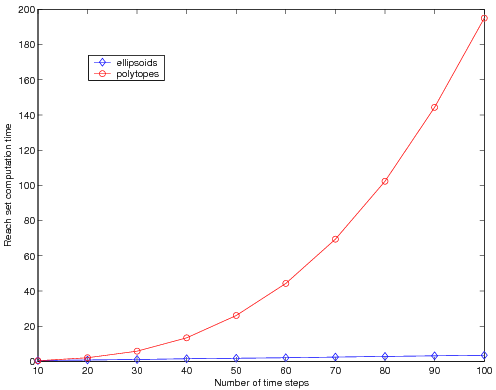
\includegraphics{ellpoly.png}
\caption{Reach set computation performance comparison.}\label{chap_examples:ellpolyfig}\end{figure}

Let ${\mathcal X}_0$ and $U$ be unit boxes in
${\bf R}^2$, and compute the reach set using the polytope method
implemented in MPT (“Multi-Parametric Toolbox Homepage”). With every
time step the number of vertices of the reach set polytope increases by
$4$. The complexity of the convex hull computation increases
exponentially with number of vertices. In \hyperref[chap_examples:ellpolyfig]{figure  \ref*{chap_examples:ellpolyfig}}, the time
required to compute the reach set for different time steps using
polytopes is shown in red.

To compute the reach set of the system using \emph{Ellipsoidal Toolbox}, we
assume ${\mathcal X}_0$ and $U$ to be unit balls in
${\bf R}^2$, fix any number of initial direction values that
corresponds to the number of ellipsoidal approximations, and obtain
external and internal ellipsoidal approximations of the reach set:

\begin{Verbatim}[commandchars=\\\{\},numbers=left,firstnumber=1,stepnumber=1]
\PYG{n}{aMat} \PYG{o}{=} \PYG{p}{[}\PYG{n}{cos}\PYG{p}{(}\PYG{l+m+mi}{1}\PYG{p}{)} \PYG{n}{sin}\PYG{p}{(}\PYG{l+m+mi}{1}\PYG{p}{)}\PYG{p}{;} \PYG{o}{\PYGZhy{}}\PYG{n}{sin}\PYG{p}{(}\PYG{l+m+mi}{1}\PYG{p}{)} \PYG{n}{cos}\PYG{p}{(}\PYG{l+m+mi}{1}\PYG{p}{)}\PYG{p}{]}\PYG{p}{;}
\PYG{n}{uBoundsEllObj} \PYG{o}{=} \PYG{n}{ell\PYGZus{}unitball}\PYG{p}{(}\PYG{l+m+mi}{2}\PYG{p}{)}\PYG{p}{;}  \PYG{o}{\PYGZpc{}} \PYG{n}{control} \PYG{n}{bounds}
\PYG{o}{\PYGZpc{}} \PYG{n}{define} \PYG{n}{linear} \PYG{n}{discrete}\PYG{o}{\PYGZhy{}}\PYG{n}{time} \PYG{n}{system}
\PYG{n}{lsys} \PYG{o}{=} \PYG{n}{elltool}\PYG{p}{.}\PYG{n}{linsys}\PYG{p}{.}\PYG{n}{LinSysFactory}\PYG{p}{.}\PYG{n}{create}\PYG{p}{(}\PYG{n}{aMat}\PYG{p}{,} \PYG{n}{eye}\PYG{p}{(}\PYG{l+m+mi}{2}\PYG{p}{)}\PYG{p}{,} \PYG{n}{uBoundsEllObj}\PYG{p}{,}\PYG{p}{.}\PYG{p}{.}\PYG{p}{.}
    \PYG{p}{[}\PYG{p}{]}\PYG{p}{,} \PYG{p}{[}\PYG{p}{]}\PYG{p}{,} \PYG{l+s+sc}{\PYGZsq{}d\PYGZsq{}}\PYG{p}{)}\PYG{p}{;}
\PYG{n}{x0EllObj} \PYG{o}{=} \PYG{n}{ell\PYGZus{}unitball}\PYG{p}{(}\PYG{l+m+mi}{2}\PYG{p}{)}\PYG{p}{;}  \PYG{o}{\PYGZpc{}} \PYG{n}{set} \PYG{n}{of} \PYG{n}{initial} \PYG{n}{conditions}
\PYG{n}{dirsMat} \PYG{o}{=} \PYG{p}{[}\PYG{n}{cos}\PYG{p}{(}\PYG{l+m+mi}{0}\PYG{o}{:}\PYG{l+m+mf}{0.1}\PYG{o}{:}\PYG{n}{pi}\PYG{p}{)}\PYG{p}{;} \PYG{n}{sin}\PYG{p}{(}\PYG{l+m+mi}{0}\PYG{o}{:}\PYG{l+m+mf}{0.1}\PYG{o}{:}\PYG{n}{pi}\PYG{p}{)}\PYG{p}{]}\PYG{p}{;}  \PYG{o}{\PYGZpc{}} \PYG{l+m+mi}{32} \PYG{n}{initial} \PYG{n}{directions}
\PYG{n}{nSteps}  \PYG{o}{=} \PYG{l+m+mi}{100}\PYG{p}{;}  \PYG{o}{\PYGZpc{}} \PYG{n}{number} \PYG{n}{of} \PYG{n}{time} \PYG{n}{steps}

\PYG{o}{\PYGZpc{}} \PYG{n}{compute} \PYG{n}{the} \PYG{n}{reach} \PYG{n}{set}
\PYG{n}{rsObj} \PYG{o}{=} \PYG{n}{elltool}\PYG{p}{.}\PYG{n}{reach}\PYG{p}{.}\PYG{n}{ReachDiscrete}\PYG{p}{(}\PYG{n}{lsys}\PYG{p}{,} \PYG{n}{x0EllObj}\PYG{p}{,} \PYG{n}{dirsMat}\PYG{p}{,} \PYG{p}{[}\PYG{l+m+mi}{0} \PYG{n}{nSteps}\PYG{p}{]}\PYG{p}{)}\PYG{p}{;}
\end{Verbatim}

In \hyperref[chap_examples:ellpolyfig]{figure  \ref*{chap_examples:ellpolyfig}}, the time required to compute both external and
internal ellipsoidal approximations, with $32$ ellipsoids each,
for different number of time steps is shown in blue.

\hyperref[chap_examples:ellpolyfig]{Figure  \ref*{chap_examples:ellpolyfig}} illustrates the fact that the complexity of polytope
method grows exponentially with number of time steps, whereas the
complexity of ellipsoidal method grows linearly.


\section{System with Disturbance}
\label{chap_examples:system-with-disturbance}\begin{figure}[htbp]
\centering
\capstart

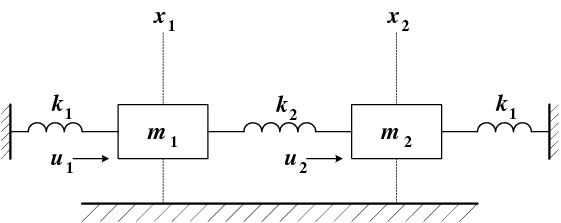
\includegraphics{springmass.png}
\caption{Spring-mass system.}\label{chap_examples:springmassfig}\end{figure}

The mechanical system presented in \hyperref[chap_examples:springmassfig]{figure  \ref*{chap_examples:springmassfig}}, is described
by the following system of equations:
\phantomsection\label{chap_examples:equation-spmass1}\begin{gather}
\begin{split}m_1\ddot{x}_1+(k_1+k_2)x_1-k_2x_2 & = & u_1,\end{split}\label{chap_examples-spmass1}
\end{gather}\phantomsection\label{chap_examples:equation-spmass2}\begin{gather}
\begin{split}m_2\ddot{x}_2-k_2x_1+(k_1+k_2)x_2 & = & u_2 .\end{split}\label{chap_examples-spmass2}
\end{gather}
Here $u_1$ and $u_2$ are the forces applied to masses
$m_1$ and $m_2$, and we shall assume
$[u_1 ~~ u_2]^T\in{\mathcal E}(0,I)$. The initial conditions can
be taken as $x_1(0)=0$, $x_2(0)=2$. Defining
$x_3=\dot{x}_1$ and $x_4=\dot{x}_2$, we can rewrite
\eqref{chap_examples-spmass1}-\eqref{chap_examples-spmass2} as a linear system in standard form:
\phantomsection\label{chap_examples:equation-spmassls}\begin{gather}
\begin{split}\left[\begin{array}{c}
\dot{x}_1 \\
\dot{x}_2 \\
\dot{x}_3 \\
\dot{x}_4 \end{array}\right] = \left[\begin{array}{cccc}
0 & 0 & 1 & 0\\
0 & 0 & 0 & 1\\
-\frac{k_1+k_2}{m_1} & \frac{k_2}{m_1} & 0 & 0\\
\frac{k_2}{m_2} & -\frac{k_1+k_2}{m_2} & 0 & 0\end{array}\right]
\left[\begin{array}{c}
x_1 \\
x_2 \\
x_3 \\
x_4 \end{array}\right] + \left[\begin{array}{cc}
0 & 0\\
0 & 0\\
\frac{1}{m_1} & 0\\
0 & \frac{1}{m_2}\end{array}\right]\left[\begin{array}{c}
u_1\\
u_2\end{array}\right].\end{split}\label{chap_examples-spmassls}
\end{gather}
Now we can compute the reach set of system \eqref{chap_examples-spmass1}-\eqref{chap_examples-spmass2} for
given time by computing the reach set of the linear system \eqref{chap_examples-spmassls}
and taking its projection onto $(x_1, x_2)$ subspace.
\begin{figure}[htbp]
\centering
\capstart

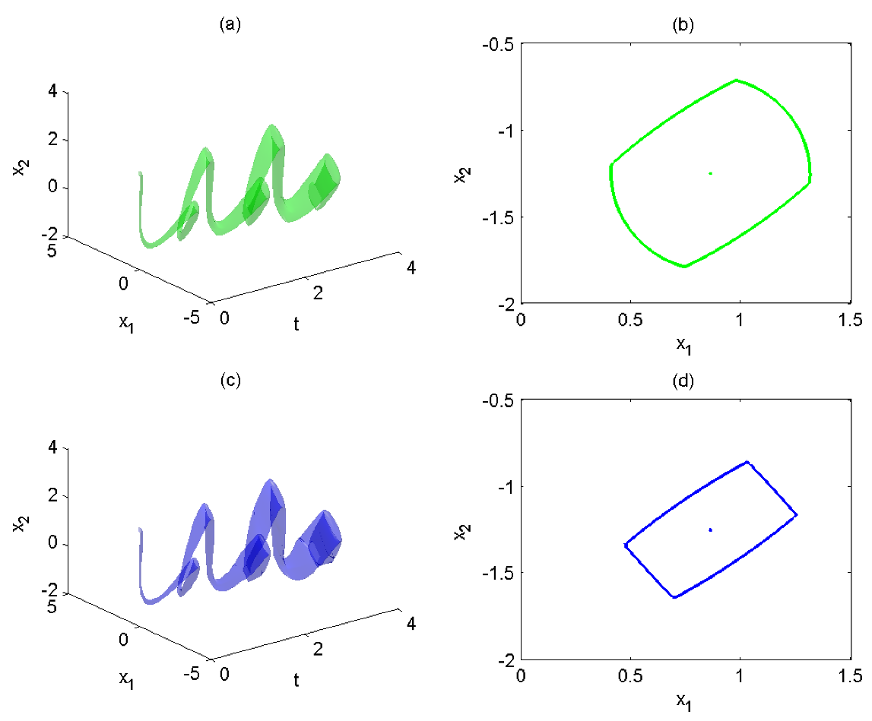
\includegraphics{reachmech.png}
\caption{Spring-mass system without disturbance:
(a) reach tube for time $t\in[0,4]$; (b) reach set at time $t=4$.
Spring-mass system with disturbance:
(c) reach tube for time $t\in[0,4]$; (d) reach set at time $t=4$.}\label{chap_examples:mechreachfig}\end{figure}

\begin{Verbatim}[commandchars=\\\{\},numbers=left,firstnumber=1,stepnumber=1]
\PYG{n}{k1} \PYG{o}{=} \PYG{l+m+mi}{24}\PYG{p}{;}  \PYG{n}{k2} \PYG{o}{=} \PYG{l+m+mi}{32}\PYG{p}{;}
\PYG{n}{m1} \PYG{o}{=} \PYG{l+m+mf}{1.5}\PYG{p}{;} \PYG{n}{m2} \PYG{o}{=} \PYG{l+m+mi}{1}\PYG{p}{;}
\PYG{o}{\PYGZpc{}} \PYG{n}{define} \PYG{n}{matrices} \PYG{n}{aMat}\PYG{p}{,} \PYG{n}{bMat}\PYG{p}{,} \PYG{n}{and} \PYG{n}{control} \PYG{n}{bounds} \PYG{n}{uBoundsEll}\PYG{o}{:}
\PYG{n}{aMat} \PYG{o}{=} \PYG{p}{[}\PYG{l+m+mi}{0} \PYG{l+m+mi}{0} \PYG{l+m+mi}{1} \PYG{l+m+mi}{0}\PYG{p}{;} \PYG{l+m+mi}{0} \PYG{l+m+mi}{0} \PYG{l+m+mi}{0} \PYG{l+m+mi}{1}\PYG{p}{;} \PYG{o}{\PYGZhy{}}\PYG{p}{(}\PYG{n}{k1}\PYG{o}{+}\PYG{n}{k2}\PYG{p}{)}\PYG{o}{/}\PYG{n}{m1} \PYG{n}{k2}\PYG{o}{/}\PYG{n}{m1} \PYG{l+m+mi}{0} \PYG{l+m+mi}{0}\PYG{p}{;} \PYG{n}{k2}\PYG{o}{/}\PYG{n}{m2} \PYG{o}{\PYGZhy{}}\PYG{p}{(}\PYG{n}{k1}\PYG{o}{+}\PYG{n}{k2}\PYG{p}{)}\PYG{o}{/}\PYG{n}{m2} \PYG{l+m+mi}{0} \PYG{l+m+mi}{0}\PYG{p}{]}\PYG{p}{;}
\PYG{n}{bMat} \PYG{o}{=} \PYG{p}{[}\PYG{l+m+mi}{0} \PYG{l+m+mi}{0}\PYG{p}{;} \PYG{l+m+mi}{0} \PYG{l+m+mi}{0}\PYG{p}{;} \PYG{l+m+mi}{1}\PYG{o}{/}\PYG{n}{m1} \PYG{l+m+mi}{0}\PYG{p}{;} \PYG{l+m+mi}{0} \PYG{l+m+mi}{1}\PYG{o}{/}\PYG{n}{m2}\PYG{p}{]}\PYG{p}{;}
\PYG{n}{uBoundsEllObj} \PYG{o}{=} \PYG{n}{ell\PYGZus{}unitball}\PYG{p}{(}\PYG{l+m+mi}{2}\PYG{p}{)}\PYG{p}{;}
\PYG{o}{\PYGZpc{}} \PYG{n}{linear} \PYG{n}{system}
\PYG{n}{lsys} \PYG{o}{=} \PYG{n}{elltool}\PYG{p}{.}\PYG{n}{linsys}\PYG{p}{.}\PYG{n}{LinSysContinuous}\PYG{p}{(}\PYG{n}{aMat}\PYG{p}{,} \PYG{n}{bMat}\PYG{p}{,} \PYG{n}{uBoundsEllObj}\PYG{p}{)}\PYG{p}{;}  
\PYG{n}{timeVec} \PYG{o}{=} \PYG{p}{[}\PYG{l+m+mi}{0} \PYG{l+m+mi}{4}\PYG{p}{]}\PYG{p}{;}  \PYG{o}{\PYGZpc{}} \PYG{n}{time} \PYG{n}{interval}\PYG{o}{\PYGZpc{}} \PYG{n}{initial} \PYG{n}{conditions}\PYG{o}{:}
\PYG{n}{x0EllObj} \PYG{o}{=} \PYG{p}{[}\PYG{l+m+mi}{0} \PYG{l+m+mi}{2} \PYG{l+m+mi}{0} \PYG{l+m+mi}{0}\PYG{p}{]}\PYG{p}{.}\PYG{err}{\PYGZsq{}} \PYG{o}{+} \PYG{n}{ellipsoid}\PYG{p}{(}\PYG{p}{[}\PYG{l+m+mf}{0.01} \PYG{l+m+mi}{0} \PYG{l+m+mi}{0} \PYG{l+m+mi}{0}\PYG{p}{;} \PYG{l+m+mi}{0} \PYG{l+m+mf}{0.01} \PYG{l+m+mi}{0} \PYG{l+m+mi}{0}\PYG{p}{;} \PYG{l+m+mi}{0} \PYG{l+m+mi}{0} \PYG{l+m+mi}{0} \PYG{l+m+mi}{0}\PYG{p}{;}\PYG{p}{.}\PYG{p}{.}\PYG{p}{.}
           \PYG{l+m+mi}{0} \PYG{l+m+mi}{0} \PYG{l+m+mi}{0} \PYG{l+m+mi}{0}\PYG{p}{]}\PYG{p}{)}\PYG{p}{;}
\PYG{o}{\PYGZpc{}} \PYG{n}{initial} \PYG{n}{directions} \PYG{p}{(}\PYG{n}{some} \PYG{n}{random} \PYG{n}{vectors} \PYG{n}{in} \PYG{n}{R}\PYG{o}{\PYGZca{}}\PYG{l+m+mi}{4}\PYG{p}{)}\PYG{o}{:}
\PYG{n}{dirsMat} \PYG{o}{=} \PYG{p}{[}\PYG{l+m+mi}{1} \PYG{l+m+mi}{0} \PYG{l+m+mi}{1} \PYG{l+m+mi}{0}\PYG{p}{;} \PYG{l+m+mi}{1} \PYG{o}{\PYGZhy{}}\PYG{l+m+mi}{1} \PYG{l+m+mi}{0} \PYG{l+m+mi}{0}\PYG{p}{;} \PYG{l+m+mi}{0} \PYG{o}{\PYGZhy{}}\PYG{l+m+mi}{1} \PYG{l+m+mi}{0} \PYG{l+m+mi}{1}\PYG{p}{;} \PYG{l+m+mi}{1} \PYG{l+m+mi}{1} \PYG{o}{\PYGZhy{}}\PYG{l+m+mi}{1} \PYG{l+m+mi}{1}\PYG{p}{;} \PYG{o}{\PYGZhy{}}\PYG{l+m+mi}{1} \PYG{l+m+mi}{1} \PYG{l+m+mi}{1} \PYG{l+m+mi}{0}\PYG{p}{;} \PYG{o}{\PYGZhy{}}\PYG{l+m+mi}{2} \PYG{l+m+mi}{0} \PYG{l+m+mi}{1} \PYG{l+m+mi}{1}\PYG{p}{]}\PYG{p}{.}\PYG{err}{\PYGZsq{}}\PYG{p}{;}
\PYG{o}{\PYGZpc{}} \PYG{n}{reach} \PYG{n}{set}
\PYG{n}{rsObj} \PYG{o}{=} \PYG{n}{elltool}\PYG{p}{.}\PYG{n}{reach}\PYG{p}{.}\PYG{n}{ReachContinuous}\PYG{p}{(}\PYG{n}{lsys}\PYG{p}{,} \PYG{n}{x0EllObj}\PYG{p}{,} \PYG{n}{dirsMat}\PYG{p}{,} \PYG{n}{timeVec}\PYG{p}{,}\PYG{p}{.}\PYG{p}{.}\PYG{p}{.}
    \PYG{err}{\PYGZsq{}}\PYG{n}{isRegEnabled}\PYG{err}{\PYGZsq{}}\PYG{p}{,} \PYG{n+nb}{true}\PYG{p}{,} \PYG{err}{\PYGZsq{}}\PYG{n}{isJustCheck}\PYG{err}{\PYGZsq{}}\PYG{p}{,} \PYG{n+nb}{false}\PYG{p}{,} \PYG{err}{\PYGZsq{}}\PYG{n}{regTol}\PYG{err}{\PYGZsq{}}\PYG{p}{,} \PYG{l+m+mf}{1e\PYGZhy{}3}\PYG{p}{)}\PYG{p}{;}  
\PYG{n}{basisMat} \PYG{o}{=} \PYG{p}{[}\PYG{l+m+mi}{1} \PYG{l+m+mi}{0} \PYG{l+m+mi}{0} \PYG{l+m+mi}{0}\PYG{p}{;} \PYG{l+m+mi}{0} \PYG{l+m+mi}{1} \PYG{l+m+mi}{0} \PYG{l+m+mi}{0}\PYG{p}{]}\PYG{err}{\PYGZsq{}}\PYG{p}{;}  \PYG{o}{\PYGZpc{}} \PYG{n}{orthogonal} \PYG{n}{basis} \PYG{n}{of} \PYG{p}{(}\PYG{n}{x1}\PYG{p}{,} \PYG{n}{x2}\PYG{p}{)} \PYG{n}{subspace}
\PYG{n}{psObj} \PYG{o}{=} \PYG{n}{rsObj}\PYG{p}{.}\PYG{n}{projection}\PYG{p}{(}\PYG{n}{basisMat}\PYG{p}{)}\PYG{p}{;}  \PYG{o}{\PYGZpc{}} \PYG{n}{reach} \PYG{n}{set} \PYG{n}{projection}
\PYG{o}{\PYGZpc{}} \PYG{n}{plot} \PYG{n}{projection} \PYG{n}{of} \PYG{n}{reach} \PYG{n}{set} \PYG{n}{external} \PYG{n}{approximation}\PYG{o}{:}

\PYG{n}{psObj}\PYG{p}{.}\PYG{n}{plotByEa}\PYG{p}{(}\PYG{l+s+sc}{\PYGZsq{}g\PYGZsq{}}\PYG{p}{)}\PYG{p}{;}  \PYG{o}{\PYGZpc{}} \PYG{n}{plot} \PYG{n}{the} \PYG{n}{whole} \PYG{n}{reach} \PYG{n}{tube}

\PYG{o}{\PYGZpc{}}
\PYG{o}{\PYGZpc{}} \PYG{n}{ReachContinuous}\PYG{err}{\PYGZsq{}}\PYG{n}{s} \PYG{n}{cut}\PYG{p}{(}\PYG{p}{)} \PYG{n}{doesn}\PYG{err}{\PYGZsq{}}\PYG{n}{t} \PYG{n}{work} \PYG{n}{with} \PYG{n}{projections}\PYG{o}{:}
\PYG{n}{psObj} \PYG{o}{=} \PYG{n}{psObj}\PYG{p}{.}\PYG{n}{cut}\PYG{p}{(}\PYG{l+m+mi}{4}\PYG{p}{)}\PYG{p}{;}
\PYG{n}{psObj}\PYG{p}{.}\PYG{n}{plotByEa}\PYG{p}{(}\PYG{l+s+sc}{\PYGZsq{}g\PYGZsq{}}\PYG{p}{)}\PYG{p}{;}  \PYG{o}{\PYGZpc{}} \PYG{n}{plot} \PYG{n}{reach} \PYG{n}{set} \PYG{n}{approximation} \PYG{n}{at} \PYG{n}{time} \PYG{n}{t} \PYG{o}{=} \PYG{l+m+mi}{4}
\end{Verbatim}

\hyperref[chap_examples:mechreachfig]{Figure  \ref*{chap_examples:mechreachfig}} (a) shows the reach set of the system
\eqref{chap_examples-spmass1}-\eqref{chap_examples-spmass2} evolving in time from $t=0$ to $t=4$.
\hyperref[chap_examples:mechreachfig]{Figure  \ref*{chap_examples:mechreachfig}} (b) presents a snapshot of this reach set at time
$t=4$.

So far we considered an ideal system without any disturbance, such as
friction. We introduce disturbance to \eqref{chap_examples-spmass1}-\eqref{chap_examples-spmass2} by adding
extra terms, $v_1$ and $v_2$,
\phantomsection\label{chap_examples:equation-smdist1}\begin{gather}
\begin{split}m_1\ddot{x}_1+(k_1+k_2)x_1-k_2x_2 & = & u_1 + v_1,\end{split}\label{chap_examples-smdist1}
\end{gather}\phantomsection\label{chap_examples:equation-smdist2}\begin{gather}
\begin{split}m_2\ddot{x}_2-k_2x_1+(k_1+k_2)x_2 & = & u_2 + v_2,\end{split}\label{chap_examples-smdist2}
\end{gather}
which results in equation \eqref{chap_examples-spmassls} getting an extra term
\begin{gather}
\begin{split}\left[\begin{array}{cc}
0 & 0\\
0 & 0\\
1 & 0\\
0 & 1\end{array}\right]\left[\begin{array}{c}
v_1\\
v_2\end{array}\right].\end{split}\notag
\end{gather}
Assuming that $[v_1 ~~ v_2]^T$ is unknown but bounded by
ellipsoid ${\mathcal E}(0, \frac{1}{4}I)$, we can compute the
closed-loop reach set of the system with disturbance.

\begin{Verbatim}[commandchars=\\\{\},numbers=left,firstnumber=1,stepnumber=1]
\PYG{c}{\PYGZpc{} define disturbance:}
\PYG{n}{gMat} \PYG{p}{=} \PYG{p}{[}\PYG{l+m+mi}{0} \PYG{l+m+mi}{0}\PYG{p}{;} \PYG{l+m+mi}{0} \PYG{l+m+mi}{0}\PYG{p}{;} \PYG{l+m+mi}{1} \PYG{l+m+mi}{0}\PYG{p}{;} \PYG{l+m+mi}{0} \PYG{l+m+mi}{1}\PYG{p}{]}\PYG{p}{;}
\PYG{n}{vEllObj} \PYG{p}{=} \PYG{l+m+mf}{0.05}\PYG{o}{*}\PYG{n}{ell\PYGZus{}unitball}\PYG{p}{(}\PYG{l+m+mi}{2}\PYG{p}{)}\PYG{p}{;}
\PYG{c}{\PYGZpc{} linear system with disturbance}
\PYG{n}{lsysd} \PYG{p}{=} \PYG{n}{elltool}\PYG{p}{.}\PYG{n}{linsys}\PYG{p}{.}\PYG{n}{LinSysContinuous}\PYG{p}{(}\PYG{n}{aMat}\PYG{p}{,} \PYG{n}{bMat}\PYG{p}{,} \PYG{n}{uBoundsEllObj}\PYG{p}{,}\PYG{c}{...}
    \PYG{n}{gMat}\PYG{p}{,} \PYG{n}{vEllObj}\PYG{p}{)}\PYG{p}{;} 
\PYG{c}{\PYGZpc{} reach set}
\PYG{n}{rsdObj} \PYG{p}{=} \PYG{n}{elltool}\PYG{p}{.}\PYG{n}{reach}\PYG{p}{.}\PYG{n}{ReachContinuous}\PYG{p}{(}\PYG{n}{lsysd}\PYG{p}{,} \PYG{n}{x0EllObj}\PYG{p}{,} \PYG{n}{dirsMat}\PYG{p}{,}\PYG{c}{...}
    \PYG{n}{timeVec}\PYG{p}{,} \PYG{l+s}{\PYGZsq{}}\PYG{l+s}{isRegEnabled\PYGZsq{}}\PYG{p}{,} \PYG{n}{true}\PYG{p}{,} \PYG{l+s}{\PYGZsq{}}\PYG{l+s}{isJustCheck\PYGZsq{}}\PYG{p}{,} \PYG{n}{false}\PYG{p}{,} \PYG{l+s}{\PYGZsq{}}\PYG{l+s}{regTol\PYGZsq{}}\PYG{p}{,} \PYG{l+m+mf}{1e\PYGZhy{}1}\PYG{p}{)}\PYG{p}{;} 
\PYG{n}{psdObj} \PYG{p}{=} \PYG{n}{rsdObj}\PYG{p}{.}\PYG{n}{projection}\PYG{p}{(}\PYG{n}{basisMat}\PYG{p}{)}\PYG{p}{;}  \PYG{c}{\PYGZpc{} reach set projection onto (x1, x2)}
\PYG{c}{\PYGZpc{} plot projection of reach set external approximation:}
\PYG{n}{psdObj}\PYG{p}{.}\PYG{n}{plotEa}\PYG{p}{(}\PYG{p}{)}\PYG{p}{;}  \PYG{c}{\PYGZpc{} plot the whole reach tube}
\PYG{n}{psdCutObj} \PYG{p}{=} \PYG{n}{psdObj}\PYG{p}{.}\PYG{n}{cut}\PYG{p}{(}\PYG{l+m+mi}{4}\PYG{p}{)}\PYG{p}{;}
\PYG{n}{psdCutObj}\PYG{p}{.}\PYG{n}{plotEa}\PYG{p}{(}\PYG{p}{)}\PYG{p}{;}  \PYG{c}{\PYGZpc{} plot reach set approximation at time t = 4}
\end{Verbatim}

\hyperref[chap_examples:mechreachfig`(c) shows the reach set of the system ([smdist1]-[smdist2]) evolving in time from :math:`t=0]{Figure  \ref*{chap_examples:mechreachfig`(c) shows the reach set of the system ([smdist1]-[smdist2]) evolving in time from :math:`t=0}} to $t=4$.
\hyperref[chap_examples:mechreachfig`(d) presents a snapshot of this reach set at time :math:`t=4]{Figure  \ref*{chap_examples:mechreachfig`(d) presents a snapshot of this reach set at time :math:`t=4}}.


\section{Switched System}
\label{chap_examples:switched-system}\begin{figure}[htbp]
\centering
\capstart

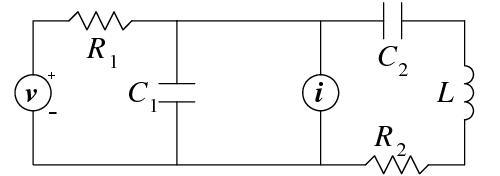
\includegraphics{rlc.png}
\caption{RLC circuit with two inputs.}\label{chap_examples:rlcfig}\end{figure}

By \emph{switched systems} we mean systems whose dynamics changes at known
times. Consider the RLC circuit shown in \hyperref[chap_examples:rlcfig]{figure  \ref*{chap_examples:rlcfig}}. It has two
inputs - the voltage ($v$) and current ($i$) sources. Define
\begin{itemize}
\item {} 
$x_1$ - voltage across capacitor $C_1$, so
$C_1\dot{x}_1$ is the corresponding current;

\item {} 
$x_2$ - voltage across capacitor $C_2$, so the
corresponding current is $C_2\dot{x}_2$.

\item {} 
$x_3$ - current through the inductor $L$, so the voltage
across the inductor is $L\dot{x}_3$.

\end{itemize}

Applying Kirchoff current and voltage laws we arrive at the linear
system,
\phantomsection\label{chap_examples:equation-rlceq}\begin{gather}
\begin{split}\left[\begin{array}{c}
\dot{x}_1\\
\dot{x}_2\\
\dot{x}_3\end{array}\right] = \left[\begin{array}{ccc}
-\frac{1}{R_1C_1} & 0 & -\frac{1}{C_1}\\
0 & 0 & \frac{1}{C_2}\\
\frac{1}{L} & -\frac{1}{L} & -\frac{R_2}{L}\end{array}\right]
\left[\begin{array}{c}
x_1\\
x_2\\
x_3\end{array}\right] + \left[\begin{array}{cc}
\frac{1}{R_1C_1} & \frac{1}{C_1}\\
0 & 0\\
0 & 0\end{array}\right]\left[\begin{array}{c}
v\\
i\end{array}\right].\end{split}\label{chap_examples-rlceq}
\end{gather}
The parameters $R_1$, $R_2$, $C_1$, $C_2$ and
$L$, as well as the inputs, may depend on time. Suppose, for time
$0\leqslant t<2$, $R_1=2$ Ohm, $R_2=1$ Ohm,
$C_1=3$ F, $C_2=7$ F, $L=2$ H, both inputs, $v$
and $i$ are present and bounded by ellipsoid
${\mathcal E}(0,I)$; and for time $t\geqslant2$,
$R_1=R_2=2$ Ohm, $C_1=C_2=3$ F, $L=6$ H, the current
source is turned off, and $|v|\leqslant1$. Then, system \eqref{chap_examples-rlceq}
can be rewritten as
\phantomsection\label{chap_examples:equation-rlceq2}\begin{gather}
\begin{split}\left[\begin{array}{c}
\dot{x}_1\\
\dot{x}_2\\
\dot{x}_3\end{array}\right] = \left\{\begin{array}{ll}
\left[\begin{array}{ccc}
-\frac{1}{6} & 0 & -\frac{1}{3}\\
0 & 0 & \frac{1}{7}\\
\frac{1}{2} & -\frac{1}{2} & -\frac{1}{2}\end{array}\right]
\left[\begin{array}{c}
x_1\\
x_2\\
x_3\end{array}\right] + \left[\begin{array}{cc}
\frac{1}{6} & \frac{1}{3}\\
0 & 0\\
0 & 0\end{array}\right]\left[\begin{array}{c}
v\\
i\end{array}\right], & 0\leqslant t< 2, \\
\left[\begin{array}{ccc}
-\frac{1}{6} & 0 & -\frac{1}{3}\\
0 & 0 & \frac{1}{3}\\
\frac{1}{6} & -\frac{1}{6} & -\frac{1}{3}\end{array}\right]
\left[\begin{array}{c}
x_1\\
x_2\\
x_3\end{array}\right] + \left[\begin{array}{c}
\frac{1}{6} \\
0 \\
0 \end{array}\right]v, & 2\leqslant t. \end{array}\right.\end{split}\label{chap_examples-rlceq2}
\end{gather}
We can compute the reach set of \eqref{chap_examples-rlceq2} for some time $t>2$,
say, $t=3$.

\begin{Verbatim}[commandchars=\\\{\},numbers=left,firstnumber=1,stepnumber=1]
\PYG{c}{\PYGZpc{} define system 1}
\PYG{n}{firstAMat} \PYG{p}{=} \PYG{p}{[}\PYG{o}{\PYGZhy{}}\PYG{l+m+mi}{1}\PYG{o}{/}\PYG{l+m+mi}{6} \PYG{l+m+mi}{0} \PYG{o}{\PYGZhy{}}\PYG{l+m+mi}{1}\PYG{o}{/}\PYG{l+m+mi}{3}\PYG{p}{;} \PYG{l+m+mi}{0} \PYG{l+m+mi}{0} \PYG{l+m+mi}{1}\PYG{o}{/}\PYG{l+m+mi}{7}\PYG{p}{;} \PYG{l+m+mi}{1}\PYG{o}{/}\PYG{l+m+mi}{2} \PYG{o}{\PYGZhy{}}\PYG{l+m+mi}{1}\PYG{o}{/}\PYG{l+m+mi}{2} \PYG{o}{\PYGZhy{}}\PYG{l+m+mi}{1}\PYG{o}{/}\PYG{l+m+mi}{2}\PYG{p}{]}\PYG{p}{;}
\PYG{n}{firstBMat} \PYG{p}{=} \PYG{p}{[}\PYG{l+m+mi}{1}\PYG{o}{/}\PYG{l+m+mi}{6} \PYG{l+m+mi}{1}\PYG{o}{/}\PYG{l+m+mi}{3}\PYG{p}{;} \PYG{l+m+mi}{0} \PYG{l+m+mi}{0}\PYG{p}{;} \PYG{l+m+mi}{0} \PYG{l+m+mi}{0}\PYG{p}{]}\PYG{p}{;}
\PYG{n}{firstUBoundsEllObj} \PYG{p}{=} \PYG{n}{ellipsoid}\PYG{p}{(}\PYG{n+nb}{eye}\PYG{p}{(}\PYG{l+m+mi}{2}\PYG{p}{)}\PYG{p}{)}\PYG{p}{;}
\PYG{n}{firstSys} \PYG{p}{=} \PYG{n}{elltool}\PYG{p}{.}\PYG{n}{linsys}\PYG{p}{.}\PYG{n}{LinSysContinuous}\PYG{p}{(}\PYG{n}{firstAMat}\PYG{p}{,} \PYG{n}{firstBMat}\PYG{p}{,}\PYG{c}{...}
       \PYG{n}{firstUBoundsEllObj}\PYG{p}{)}\PYG{p}{;}
\PYG{c}{\PYGZpc{} define system 2:}
\PYG{n}{secAMat} \PYG{p}{=} \PYG{p}{[}\PYG{o}{\PYGZhy{}}\PYG{l+m+mi}{1}\PYG{o}{/}\PYG{l+m+mi}{6} \PYG{l+m+mi}{0} \PYG{o}{\PYGZhy{}}\PYG{l+m+mi}{1}\PYG{o}{/}\PYG{l+m+mi}{3}\PYG{p}{;} \PYG{l+m+mi}{0} \PYG{l+m+mi}{0} \PYG{l+m+mi}{1}\PYG{o}{/}\PYG{l+m+mi}{3}\PYG{p}{;} \PYG{l+m+mi}{1}\PYG{o}{/}\PYG{l+m+mi}{6} \PYG{o}{\PYGZhy{}}\PYG{l+m+mi}{1}\PYG{o}{/}\PYG{l+m+mi}{6} \PYG{o}{\PYGZhy{}}\PYG{l+m+mi}{1}\PYG{o}{/}\PYG{l+m+mi}{3}\PYG{p}{]}\PYG{p}{;}
\PYG{n}{secBMat} \PYG{p}{=} \PYG{p}{[}\PYG{l+m+mi}{1}\PYG{o}{/}\PYG{l+m+mi}{6}\PYG{p}{;} \PYG{l+m+mi}{0}\PYG{p}{;} \PYG{l+m+mi}{0}\PYG{p}{]}\PYG{p}{;}
\PYG{n}{secUBoundsEllObj} \PYG{p}{=} \PYG{n}{ellipsoid}\PYG{p}{(}\PYG{l+m+mi}{1}\PYG{p}{)}\PYG{p}{;}
\PYG{n}{secondSys} \PYG{p}{=} \PYG{n}{elltool}\PYG{p}{.}\PYG{n}{linsys}\PYG{p}{.}\PYG{n}{LinSysContinuous}\PYG{p}{(}\PYG{n}{secAMat}\PYG{p}{,} \PYG{n}{secBMat}\PYG{p}{,}\PYG{c}{....}
         \PYG{n}{secUBoundsEllObj}\PYG{p}{)}\PYG{p}{;}
\PYG{n}{x0EllObj} \PYG{p}{=} \PYG{n}{ellipsoid}\PYG{p}{(}\PYG{l+m+mf}{0.01}\PYG{o}{*}\PYG{n+nb}{eye}\PYG{p}{(}\PYG{l+m+mi}{3}\PYG{p}{)}\PYG{p}{)}\PYG{p}{;}  \PYG{c}{\PYGZpc{} set of initial states}
\PYG{n}{dirsMat} \PYG{p}{=} \PYG{n+nb}{eye}\PYG{p}{(}\PYG{l+m+mi}{3}\PYG{p}{)}\PYG{p}{;}  \PYG{c}{\PYGZpc{} 3 initial directions}
\PYG{n}{switchTime} \PYG{p}{=} \PYG{l+m+mi}{2}\PYG{p}{;}  \PYG{c}{\PYGZpc{} time of switch}
\PYG{n}{termTime} \PYG{p}{=} \PYG{l+m+mi}{3}\PYG{p}{;}  \PYG{c}{\PYGZpc{} terminating time}

\PYG{c}{\PYGZpc{} compute the reach set:}
\PYG{n}{firstRsObj} \PYG{p}{=} \PYG{n}{elltool}\PYG{p}{.}\PYG{n}{reach}\PYG{p}{.}\PYG{n}{ReachContinuous}\PYG{p}{(}\PYG{n}{firstSys}\PYG{p}{,} \PYG{n}{x0EllObj}\PYG{p}{,} \PYG{n}{dirsMat}\PYG{p}{,}\PYG{c}{...}
 \PYG{p}{[}\PYG{l+m+mi}{0} \PYG{n}{switchTime}\PYG{p}{]}\PYG{p}{,} \PYG{l+s}{\PYGZsq{}}\PYG{l+s}{isRegEnabled\PYGZsq{}}\PYG{p}{,} \PYG{n}{true}\PYG{p}{,} \PYG{l+s}{\PYGZsq{}}\PYG{l+s}{isJustCheck\PYGZsq{}}\PYG{p}{,} \PYG{n}{false}\PYG{p}{,}\PYG{c}{...}
 \PYG{l+s}{\PYGZsq{}}\PYG{l+s}{regTol\PYGZsq{}}\PYG{p}{,} \PYG{l+m+mf}{1e\PYGZhy{}5}\PYG{p}{)}\PYG{p}{;}  \PYG{c}{\PYGZpc{} reach set of the first system}
\PYG{c}{\PYGZpc{} computation of the second reach set starts}
\PYG{c}{\PYGZpc{} where the first left off}
\PYG{n}{secRsObj} \PYG{p}{=} \PYG{n}{firstRsObj}\PYG{p}{.}\PYG{n}{evolve}\PYG{p}{(}\PYG{n}{termTime}\PYG{p}{,} \PYG{n}{secondSys}\PYG{p}{)}\PYG{p}{;}

\PYG{c}{\PYGZpc{} obtain projections onto (x1, x2) subspace:}
\PYG{n}{basisMat} \PYG{p}{=} \PYG{p}{[}\PYG{l+m+mi}{1} \PYG{l+m+mi}{0} \PYG{l+m+mi}{0}\PYG{p}{;} \PYG{l+m+mi}{0} \PYG{l+m+mi}{1} \PYG{l+m+mi}{0}\PYG{p}{]}\PYG{o}{\PYGZsq{}}\PYG{p}{;}  \PYG{c}{\PYGZpc{} (x1, x2) subspace basis}
\PYG{n}{firstPsObj} \PYG{p}{=} \PYG{n}{firstRsObj}\PYG{p}{.}\PYG{n}{projection}\PYG{p}{(}\PYG{n}{basisMat}\PYG{p}{)}\PYG{p}{;}
\PYG{n}{secPsObj} \PYG{p}{=} \PYG{n}{secRsObj}\PYG{p}{.}\PYG{n}{projection}\PYG{p}{(}\PYG{n}{basisMat}\PYG{p}{)}\PYG{p}{;}

\PYG{c}{\PYGZpc{} plot the results:}

\PYG{n}{firstPsObj}\PYG{p}{.}\PYG{n}{plotByEa}\PYG{p}{(}\PYG{l+s}{\PYGZsq{}}\PYG{l+s}{r\PYGZsq{}}\PYG{p}{)}\PYG{p}{;}  \PYG{c}{\PYGZpc{} external apprx. of reach set 1 (red)}
\PYG{n}{hold} \PYG{n}{on}\PYG{p}{;}
\PYG{n}{firstPsObj}\PYG{p}{.}\PYG{n}{plotByIa}\PYG{p}{(}\PYG{l+s}{\PYGZsq{}}\PYG{l+s}{g\PYGZsq{}}\PYG{p}{)}\PYG{p}{;}  \PYG{c}{\PYGZpc{} internal apprx. of reach set 1 (green)}
\PYG{n}{secPsObj}\PYG{p}{.}\PYG{n}{plotByEa}\PYG{p}{(}\PYG{l+s}{\PYGZsq{}}\PYG{l+s}{y\PYGZsq{}}\PYG{p}{)}\PYG{p}{;}  \PYG{c}{\PYGZpc{} external apprx. of reach set 2 (yellow)}
\PYG{n}{secPsObj}\PYG{p}{.}\PYG{n}{plotByIa}\PYG{p}{(}\PYG{l+s}{\PYGZsq{}}\PYG{l+s}{b\PYGZsq{}}\PYG{p}{)}\PYG{p}{;}  \PYG{c}{\PYGZpc{} internal apprx. of reach set 2 (blue)}
\PYG{c}{\PYGZpc{} plot the 3\PYGZhy{}dimensional reach set at time t = 3:}
\PYG{n}{secRsObj} \PYG{p}{=} \PYG{n}{secRsObj}\PYG{p}{.}\PYG{n}{cut}\PYG{p}{(}\PYG{l+m+mi}{3}\PYG{p}{)}\PYG{p}{;}
\PYG{n}{secRsObj}\PYG{p}{.}\PYG{n}{plotByEa}\PYG{p}{(}\PYG{l+s}{\PYGZsq{}}\PYG{l+s}{y\PYGZsq{}}\PYG{p}{)}\PYG{p}{;}
\PYG{n}{hold} \PYG{n}{on}\PYG{p}{;}
\PYG{n}{secRsObj}\PYG{p}{.}\PYG{n}{plotByIa}\PYG{p}{(}\PYG{l+s}{\PYGZsq{}}\PYG{l+s}{b\PYGZsq{}}\PYG{p}{)}\PYG{p}{;}
\end{Verbatim}
\begin{figure}[htbp]
\centering
\capstart

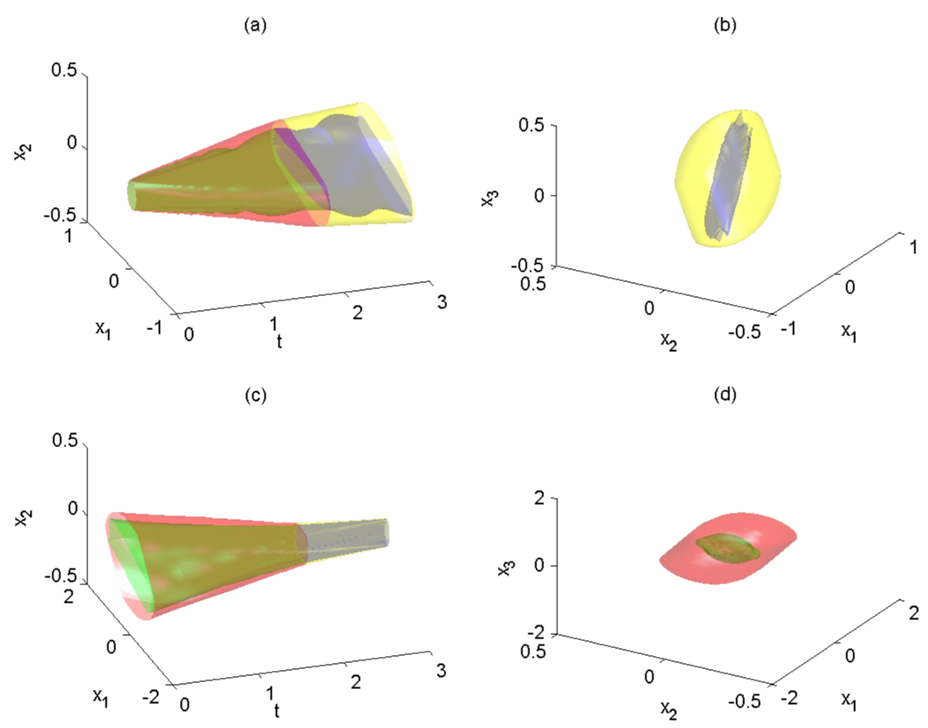
\includegraphics{rlcreach.png}
\caption{Forward and backward reach sets of the switched system
(external and internal approximations).}\label{chap_examples:rlcreachfig}\end{figure}

\hyperref[chap_examples:rlcreachfig]{Figure  \ref*{chap_examples:rlcreachfig}} (a) shows how the reach set projection onto
$(x_1, x_2)$ of system \eqref{chap_examples-rlceq2} evolves in time from $t=0$
to $t=3$. The external reach set approximation for the first
dynamics is in red, the internal approximation is in green. The dynamics
switches at $t=2$. The external reach set approximation for the
second dynamics is in yellow, its internal approximation is in blue. The
full three-dimensional external (yellow) and internal (blue)
approximations of the reach set are shown in \hyperref[chap_examples:rlcreachfig]{figure  \ref*{chap_examples:rlcreachfig}} (b).

To find out where the system should start at time $t=0$ in order
to reach a neighborhood M of the origin at time $t=3$, we compute
the backward reach set from $t=3$ to $t=0$.

\begin{Verbatim}[commandchars=\\\{\},numbers=left,firstnumber=1,stepnumber=1]
\PYG{n}{mEllObj}  \PYG{o}{=} \PYG{n}{ellipsoid}\PYG{p}{(}\PYG{l+m+mf}{0.01}\PYG{o}{*}\PYG{n}{eye}\PYG{p}{(}\PYG{l+m+mi}{3}\PYG{p}{)}\PYG{p}{)}\PYG{p}{;}  \PYG{o}{\PYGZpc{}} \PYG{n}{terminating} \PYG{n}{set}
\PYG{n}{termTime} \PYG{o}{=} \PYG{l+m+mi}{3}\PYG{p}{;}  \PYG{o}{\PYGZpc{}} \PYG{n}{terminating} \PYG{n}{time}

\PYG{o}{\PYGZpc{}} \PYG{n}{compute} \PYG{n}{backward} \PYG{n}{reach} \PYG{n}{set}\PYG{o}{:}
\PYG{o}{\PYGZpc{}} \PYG{n}{compute} \PYG{n}{the} \PYG{n}{reach} \PYG{n}{set}\PYG{o}{:}
\PYG{n}{secBrsObj} \PYG{o}{=} \PYG{n}{elltool}\PYG{p}{.}\PYG{n}{reach}\PYG{p}{.}\PYG{n}{ReachContinuous}\PYG{p}{(}\PYG{n}{secondSys}\PYG{p}{,} \PYG{n}{mEllObj}\PYG{p}{,} \PYG{n}{dirsMat}\PYG{p}{,}\PYG{p}{.}\PYG{p}{.}\PYG{p}{.}
 \PYG{p}{[}\PYG{n}{termTime} \PYG{n}{switchTime}\PYG{p}{]}\PYG{p}{,} \PYG{err}{\PYGZsq{}}\PYG{n}{isRegEnabled}\PYG{err}{\PYGZsq{}}\PYG{p}{,} \PYG{n+nb}{true}\PYG{p}{,} \PYG{err}{\PYGZsq{}}\PYG{n}{isJustCheck}\PYG{err}{\PYGZsq{}}\PYG{p}{,} \PYG{n+nb}{false}\PYG{p}{,}\PYG{p}{.}\PYG{p}{.}\PYG{p}{.}
 \PYG{err}{\PYGZsq{}}\PYG{n}{regTol}\PYG{err}{\PYGZsq{}}\PYG{p}{,} \PYG{l+m+mf}{1e\PYGZhy{}5}\PYG{p}{)}\PYG{p}{;}  \PYG{o}{\PYGZpc{}} \PYG{n}{second} \PYG{n}{system} \PYG{n}{comes} \PYG{n}{first}
\PYG{n}{firstBrsObj} \PYG{o}{=} \PYG{n}{secBrsObj}\PYG{p}{.}\PYG{n}{evolve}\PYG{p}{(}\PYG{l+m+mi}{0}\PYG{p}{,} \PYG{n}{firstSys}\PYG{p}{)}\PYG{p}{;}  \PYG{o}{\PYGZpc{}} \PYG{n}{then} \PYG{n}{the} \PYG{n}{first} \PYG{n}{system}

\PYG{o}{\PYGZpc{}} \PYG{n}{obtain} \PYG{n}{projections} \PYG{n}{onto} \PYG{p}{(}\PYG{n}{x1}\PYG{p}{,} \PYG{n}{x2}\PYG{p}{)} \PYG{n}{subspace}\PYG{o}{:}
\PYG{n}{firstBpsObj} \PYG{o}{=} \PYG{n}{firstBrsObj}\PYG{p}{.}\PYG{n}{projection}\PYG{p}{(}\PYG{n}{basisMat}\PYG{p}{)}\PYG{p}{;}
\PYG{n}{secBpsObj} \PYG{o}{=} \PYG{n}{secBrsObj}\PYG{p}{.}\PYG{n}{projection}\PYG{p}{(}\PYG{n}{basisMat}\PYG{p}{)}\PYG{p}{;}

\PYG{o}{\PYGZpc{}} \PYG{n}{plot} \PYG{n}{the} \PYG{n}{results}\PYG{o}{:}

\PYG{n}{firstBpsObj}\PYG{p}{.}\PYG{n}{plotByEa}\PYG{p}{(}\PYG{l+s+sc}{\PYGZsq{}r\PYGZsq{}}\PYG{p}{)}\PYG{p}{;} \PYG{o}{\PYGZpc{}} \PYG{n}{external} \PYG{n}{apprx}\PYG{p}{.} \PYG{n}{of} \PYG{n}{backward} \PYG{n}{reach} \PYG{n}{set} \PYG{l+m+mi}{1} \PYG{p}{(}\PYG{n}{red}\PYG{p}{)}
\PYG{n}{hold} \PYG{n}{on}\PYG{p}{;}
\PYG{n}{firstBpsObj}\PYG{p}{.}\PYG{n}{plotByIa}\PYG{p}{(}\PYG{l+s+sc}{\PYGZsq{}g\PYGZsq{}}\PYG{p}{)}\PYG{p}{;} \PYG{o}{\PYGZpc{}} \PYG{n}{internal} \PYG{n}{apprx}\PYG{p}{.} \PYG{n}{of} \PYG{n}{backward} \PYG{n}{reach} \PYG{n}{set} \PYG{l+m+mi}{1} \PYG{p}{(}\PYG{n}{green}\PYG{p}{)}
\PYG{n}{secBpsObj}\PYG{p}{.}\PYG{n}{plotByEa}\PYG{p}{(}\PYG{l+s+sc}{\PYGZsq{}y\PYGZsq{}}\PYG{p}{)}\PYG{p}{;} \PYG{o}{\PYGZpc{}} \PYG{n}{external} \PYG{n}{apprx}\PYG{p}{.} \PYG{n}{of} \PYG{n}{backward} \PYG{n}{reach} \PYG{n}{set} \PYG{l+m+mi}{2} \PYG{p}{(}\PYG{n}{yellow}\PYG{p}{)}
\PYG{n}{secBpsObj}\PYG{p}{.}\PYG{n}{plotByIa}\PYG{p}{(}\PYG{l+s+sc}{\PYGZsq{}b\PYGZsq{}}\PYG{p}{)}\PYG{p}{;} \PYG{o}{\PYGZpc{}} \PYG{n}{internal} \PYG{n}{apprx}\PYG{p}{.} \PYG{n}{of} \PYG{n}{backward} \PYG{n}{reach} \PYG{n}{set} \PYG{l+m+mi}{2} \PYG{p}{(}\PYG{n}{blue}\PYG{p}{)}

\PYG{o}{\PYGZpc{}} \PYG{n}{plot} \PYG{n}{the} \PYG{l+m+mi}{3}\PYG{o}{\PYGZhy{}}\PYG{n}{dimensional} \PYG{n}{backward} \PYG{n}{reach} \PYG{n}{set} \PYG{n}{at} \PYG{n}{time} \PYG{n}{t} \PYG{o}{=} \PYG{l+m+mi}{0}\PYG{o}{:}

\PYG{n}{firstBrsObj} \PYG{o}{=} \PYG{n}{firstBrsObj}\PYG{p}{.}\PYG{n}{cut}\PYG{p}{(}\PYG{l+m+mi}{0}\PYG{p}{)}\PYG{p}{;}
\PYG{n}{firstBrsObj}\PYG{p}{.}\PYG{n}{plotByEa}\PYG{p}{(}\PYG{l+s+sc}{\PYGZsq{}r\PYGZsq{}}\PYG{p}{)}\PYG{p}{;}
\PYG{n}{hold} \PYG{n}{on}\PYG{p}{;}
\PYG{n}{firstBrsObj}\PYG{p}{.}\PYG{n}{plotByIa}\PYG{p}{(}\PYG{l+s+sc}{\PYGZsq{}g\PYGZsq{}}\PYG{p}{)}\PYG{p}{;}
\end{Verbatim}

\hyperref[chap_examples:rlcreachfig]{Figure  \ref*{chap_examples:rlcreachfig}} (c) presents the evolution of the reach set projection onto
$(x_1, x_2)$ in backward time. Again, external and internal
approximations corresponding to the first dynamics are shown in red and
green, and to the second dynamics in yellow and blue. The full
dimensional backward reach set external and internal approximations of
system \eqref{chap_examples-rlceq2} at time $t=0$ is shown in \hyperref[chap_examples:rlcreachfig]{figure  \ref*{chap_examples:rlcreachfig}} (d).


\section{Hybrid System}
\label{chap_examples:hybrid-system}\begin{figure}[htbp]
\centering
\capstart

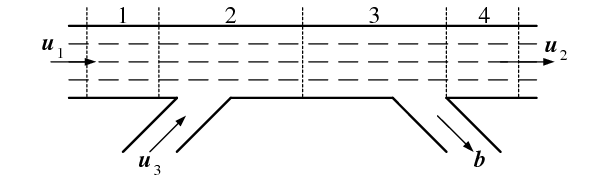
\includegraphics{hw.png}
\caption{Highway model. Adapted from L.Muñoz et al. (2003).}\label{chap_examples:hwfig}\end{figure}

There is no explicit implementation of the reachability analysis for
hybrid systems in the \emph{Ellipsoidal Toolbox}. Nonetheless, the operations
of intersection available in the toolbox allow us to work with certain
class of hybrid systems, namely, hybrid systems with affine continuous
dynamics whose guards are ellipsoids, hyperplanes, halfspaces or
polytopes.

We consider the \emph{switching-mode model} of highway traffic presented in
L.Muñoz et al. (2003). The highway segment is divided into $N$
cells as shown in \hyperref[chap_examples:hwfig]{figure  \ref*{chap_examples:hwfig}}. In this particular case, $N=4$.
The traffic density in cell $i$ is $x_i$ vehicles per mile,
$i=1,2,3,4$.

Define
\begin{itemize}
\item {} 
$v_i$ - average speed in mph, in the $i$-th cell,
$i=1,2,3,4$;

\item {} 
$w_i$ - backward congestion wave propagation speed in mph, in
the $i$-th highway cell, $i=1,2,3,4$;

\item {} 
$x_{Mi}$ - maximum allowed density in the $i$-th cell;
when this velue is reached, there is a traffic jam,
$i=1,2,3,4$;

\item {} 
$d_i$ - length of $i$-th cell in miles,
$i=1,2,3,4$;

\item {} 
$T_s$ - sampling time in hours;

\item {} 
$b$ - split ratio for the off-ramp;

\item {} 
$u_1$ - traffic flow coming into the highway segment, in
vehicles per hour (vph);

\item {} 
$u_2$ - traffic flow coming out of the highway segment (vph);

\item {} 
$u_3$ - on-ramp traffic flow (vph).

\end{itemize}

Highway traffic operates in two modes: \emph{free-flow} in normal operation;
and \emph{congested} mode, when there is a jam. Traffic flow in free-flow
mode is described by
\phantomsection\label{chap_examples:equation-fflow}\begin{gather}
\begin{split}\begin{aligned}
\left[\begin{array}{c}
x_1[t+1]\\
x_2[t+1]\\
x_3[t+1]\\
x_4[t+1]\end{array}\right] & = & \left[\begin{array}{cccc}
1-\frac{v_1T_s}{d_1} & 0 & 0 & 0\\
\frac{v_1T_s}{d_2} & 1-\frac{v_2T_s}{d_2} & 0 & 0\\
0 & \frac{v_2T_s}{d_3} & 1-\frac{v_3T_s}{d_3} & 0\\
0 & 0 & (1-b)\frac{v_3T_s}{d_4} & 1-\frac{v_4T_s}{d_4}\end{array}\right]
\left[\begin{array}{c}
x_1[t]\\
x_2[t]\\
x_3[t]\\
x_4[t]\end{array}\right] \nonumber\\
& + & \left[\begin{array}{ccc}
\frac{v_1T_s}{d_1} & 0 & 0\\
0 & 0 & \frac{v_2T_s}{d_2}\\
0 & 0 & 0\\
0 & 0 & 0\end{array}\right]\left[\begin{array}{c}
u_1\\
u_2\\
u_3\end{array}\right].\end{aligned}\end{split}\label{chap_examples-fflow}
\end{gather}
The equation for the congested mode is
\phantomsection\label{chap_examples:equation-cflow}\begin{gather}
\begin{split}\begin{aligned}
\left[\begin{array}{c}
x_1[t+1]\\
x_2[t+1]\\
x_3[t+1]\\
x_4[t+1]\end{array}\right] & = & \left[\begin{array}{cccc}
1-\frac{w_1T_s}{d_1} & \frac{w_2T_s}{d_1} & 0 & 0\\
0 & 1-\frac{w_2T_s}{d_2} & \frac{w_3T_s}{d_2} & 0\\
0 & 0 & 1-\frac{w_3T_s}{d_3} & \frac{1}{1-b}\frac{w_4T_s}{d_3}\\
0 & 0 & 0 & 1-\frac{w_4T_s}{d_4}\end{array}\right]
\left[\begin{array}{c}
x_1[t]\\
x_2[t]\\
x_3[t]\\
x_4[t]\end{array}\right] \nonumber\\
& + & \left[\begin{array}{ccc}
0 & 0 & \frac{w_1T_s}{d_1}\\
0 & 0 & 0\\
0 & 0 & 0\\
0 & -\frac{w_4T_s}{d_4} & 0\end{array}\right]\left[\begin{array}{c}
u_1\\
u_2\\
u_3\end{array}\right] \nonumber\\
& + & \left[\begin{array}{cccc}
\frac{w_1T_s}{d_1} & -\frac{w_2T_s}{d_1} & 0 & 0\\
0 & \frac{w_2T_s}{d_2} & -\frac{w_3T_s}{d_2} & 0\\
0 & 0 & \frac{w_3T_s}{d_3} & -\frac{1}{1-b}\frac{w_4T_s}{d_3}\\
0 & 0 & 0 & \frac{w_4T_s}{d_4}\end{array}\right]
\left[\begin{array}{c}
x_{M1}\\
x_{M2}\\
x_{M3}\\
x_{M4}\end{array}\right].\end{aligned}\end{split}\label{chap_examples-cflow}
\end{gather}
The switch from the free-flow to the congested mode occurs when the
density $x_2$ reaches $x_{M2}$. In other words, the
hyperplane $H([0 ~ 1 ~ 0 ~ 0]^T, x_{M2})$ is the guard.

We indicate how to implement the reach set computation of this hybrid
system. We first define the two linear systems and the guard.

\begin{Verbatim}[commandchars=\\\{\},numbers=left,firstnumber=1,stepnumber=1]
\PYG{c}{\PYGZpc{} assign parameter values:}
\PYG{n}{v1} \PYG{p}{=} \PYG{l+m+mi}{65}\PYG{p}{;} \PYG{n}{v2} \PYG{p}{=} \PYG{l+m+mi}{60}\PYG{p}{;} \PYG{n}{v3} \PYG{p}{=} \PYG{l+m+mi}{63}\PYG{p}{;} \PYG{n}{v4} \PYG{p}{=} \PYG{l+m+mi}{65}\PYG{p}{;}  \PYG{c}{\PYGZpc{} mph}
\PYG{n}{w1} \PYG{p}{=} \PYG{l+m+mi}{10}\PYG{p}{;} \PYG{n}{w2} \PYG{p}{=} \PYG{l+m+mi}{10}\PYG{p}{;} \PYG{n}{w3} \PYG{p}{=} \PYG{l+m+mi}{10}\PYG{p}{;} \PYG{n}{w4} \PYG{p}{=} \PYG{l+m+mi}{10}\PYG{p}{;}  \PYG{c}{\PYGZpc{} mph}
\PYG{n}{d1} \PYG{p}{=} \PYG{l+m+mi}{2}\PYG{p}{;} \PYG{n}{d2} \PYG{p}{=} \PYG{l+m+mi}{3}\PYG{p}{;} \PYG{n}{d3} \PYG{p}{=} \PYG{l+m+mi}{4}\PYG{p}{;} \PYG{n}{d4} \PYG{p}{=} \PYG{l+m+mi}{2}\PYG{p}{;}  \PYG{c}{\PYGZpc{} miles}
\PYG{n}{Ts} \PYG{p}{=} \PYG{l+m+mi}{2}\PYG{o}{/}\PYG{l+m+mi}{3600}\PYG{p}{;}  \PYG{c}{\PYGZpc{} sampling time in hours}
\PYG{n}{xM1} \PYG{p}{=} \PYG{l+m+mi}{200}\PYG{p}{;} \PYG{n}{xM2} \PYG{p}{=} \PYG{l+m+mi}{200}\PYG{p}{;} \PYG{n}{xM3} \PYG{p}{=} \PYG{l+m+mi}{200}\PYG{p}{;} \PYG{n}{xM4} \PYG{p}{=} \PYG{l+m+mi}{200}\PYG{p}{;}  \PYG{c}{\PYGZpc{} vehicles per lane}
\PYG{n}{b} \PYG{p}{=} \PYG{l+m+mf}{0.4}\PYG{p}{;}

\PYG{n}{firstAMat} \PYG{p}{=} \PYG{p}{[}\PYG{p}{(}\PYG{l+m+mi}{1}\PYG{o}{\PYGZhy{}}\PYG{p}{(}\PYG{n}{v1}\PYG{o}{*}\PYG{n}{Ts}\PYG{o}{/}\PYG{n}{d1}\PYG{p}{)}\PYG{p}{)} \PYG{l+m+mi}{0} \PYG{l+m+mi}{0} \PYG{l+m+mi}{0}
         \PYG{p}{(}\PYG{n}{v1}\PYG{o}{*}\PYG{n}{Ts}\PYG{o}{/}\PYG{n}{d2}\PYG{p}{)} \PYG{p}{(}\PYG{l+m+mi}{1}\PYG{o}{\PYGZhy{}}\PYG{p}{(}\PYG{n}{v2}\PYG{o}{*}\PYG{n}{Ts}\PYG{o}{/}\PYG{n}{d2}\PYG{p}{)}\PYG{p}{)} \PYG{l+m+mi}{0} \PYG{l+m+mi}{0}
         \PYG{l+m+mi}{0} \PYG{p}{(}\PYG{n}{v2}\PYG{o}{*}\PYG{n}{Ts}\PYG{o}{/}\PYG{n}{d3}\PYG{p}{)} \PYG{p}{(}\PYG{l+m+mi}{1}\PYG{o}{\PYGZhy{}}\PYG{p}{(}\PYG{n}{v3}\PYG{o}{*}\PYG{n}{Ts}\PYG{o}{/}\PYG{n}{d3}\PYG{p}{)}\PYG{p}{)} \PYG{l+m+mi}{0}
         \PYG{l+m+mi}{0} \PYG{l+m+mi}{0} \PYG{p}{(}\PYG{p}{(}\PYG{l+m+mi}{1}\PYG{o}{\PYGZhy{}}\PYG{n}{b}\PYG{p}{)}\PYG{o}{*}\PYG{p}{(}\PYG{n}{v3}\PYG{o}{*}\PYG{n}{Ts}\PYG{o}{/}\PYG{n}{d4}\PYG{p}{)}\PYG{p}{)} \PYG{p}{(}\PYG{l+m+mi}{1}\PYG{o}{\PYGZhy{}}\PYG{p}{(}\PYG{n}{v4}\PYG{o}{*}\PYG{n}{Ts}\PYG{o}{/}\PYG{n}{d4}\PYG{p}{)}\PYG{p}{)}\PYG{p}{]}\PYG{p}{;}
\PYG{n}{firstBMat} \PYG{p}{=} \PYG{p}{[}\PYG{n}{v1}\PYG{o}{*}\PYG{n}{Ts}\PYG{o}{/}\PYG{n}{d1} \PYG{l+m+mi}{0} \PYG{l+m+mi}{0}\PYG{p}{;} \PYG{l+m+mi}{0} \PYG{l+m+mi}{0} \PYG{n}{v2}\PYG{o}{*}\PYG{n}{Ts}\PYG{o}{/}\PYG{n}{d2}\PYG{p}{;} \PYG{l+m+mi}{0} \PYG{l+m+mi}{0} \PYG{l+m+mi}{0}\PYG{p}{;} \PYG{l+m+mi}{0} \PYG{l+m+mi}{0} \PYG{l+m+mi}{0}\PYG{p}{]}\PYG{p}{;}
\PYG{n}{firstUBoundsEllObj} \PYG{p}{=} \PYG{n}{ellipsoid}\PYG{p}{(}\PYG{p}{[}\PYG{l+m+mi}{180}\PYG{p}{;} \PYG{l+m+mi}{150}\PYG{p}{;} \PYG{l+m+mi}{50}\PYG{p}{]}\PYG{p}{,} \PYG{p}{[}\PYG{l+m+mi}{100} \PYG{l+m+mi}{0} \PYG{l+m+mi}{0}\PYG{p}{;} \PYG{l+m+mi}{0} \PYG{l+m+mi}{100} \PYG{l+m+mi}{0}\PYG{p}{;} \PYG{l+m+mi}{0} \PYG{l+m+mi}{0} \PYG{l+m+mi}{25}\PYG{p}{]}\PYG{p}{)}\PYG{p}{;}

\PYG{n}{secAMat} \PYG{p}{=} \PYG{p}{[}\PYG{p}{(}\PYG{l+m+mi}{1}\PYG{o}{\PYGZhy{}}\PYG{p}{(}\PYG{n}{w1}\PYG{o}{*}\PYG{n}{Ts}\PYG{o}{/}\PYG{n}{d1}\PYG{p}{)}\PYG{p}{)} \PYG{p}{(}\PYG{n}{w2}\PYG{o}{*}\PYG{n}{Ts}\PYG{o}{/}\PYG{n}{d1}\PYG{p}{)} \PYG{l+m+mi}{0} \PYG{l+m+mi}{0}
         \PYG{l+m+mi}{0} \PYG{p}{(}\PYG{l+m+mi}{1}\PYG{o}{\PYGZhy{}}\PYG{p}{(}\PYG{n}{w2}\PYG{o}{*}\PYG{n}{Ts}\PYG{o}{/}\PYG{n}{d2}\PYG{p}{)}\PYG{p}{)} \PYG{p}{(}\PYG{n}{w3}\PYG{o}{*}\PYG{n}{Ts}\PYG{o}{/}\PYG{n}{d2}\PYG{p}{)} \PYG{l+m+mi}{0}
         \PYG{l+m+mi}{0} \PYG{l+m+mi}{0} \PYG{p}{(}\PYG{l+m+mi}{1}\PYG{o}{\PYGZhy{}}\PYG{p}{(}\PYG{n}{w3}\PYG{o}{*}\PYG{n}{Ts}\PYG{o}{/}\PYG{n}{d3}\PYG{p}{)}\PYG{p}{)} \PYG{p}{(}\PYG{p}{(}\PYG{l+m+mi}{1}\PYG{o}{/}\PYG{p}{(}\PYG{l+m+mi}{1}\PYG{o}{\PYGZhy{}}\PYG{n}{b}\PYG{p}{)}\PYG{p}{)}\PYG{o}{*}\PYG{p}{(}\PYG{n}{w4}\PYG{o}{*}\PYG{n}{Ts}\PYG{o}{/}\PYG{n}{d3}\PYG{p}{)}\PYG{p}{)}
         \PYG{l+m+mi}{0} \PYG{l+m+mi}{0} \PYG{l+m+mi}{0} \PYG{p}{(}\PYG{l+m+mi}{1}\PYG{o}{\PYGZhy{}}\PYG{p}{(}\PYG{n}{w4}\PYG{o}{*}\PYG{n}{Ts}\PYG{o}{/}\PYG{n}{d4}\PYG{p}{)}\PYG{p}{)}\PYG{p}{]}\PYG{p}{;}
\PYG{n}{secBMat} \PYG{p}{=} \PYG{p}{[}\PYG{l+m+mi}{0} \PYG{l+m+mi}{0} \PYG{n}{w1}\PYG{o}{*}\PYG{n}{Ts}\PYG{o}{/}\PYG{n}{d1}\PYG{p}{;} \PYG{l+m+mi}{0} \PYG{l+m+mi}{0} \PYG{l+m+mi}{0}\PYG{p}{;} \PYG{l+m+mi}{0} \PYG{l+m+mi}{0} \PYG{l+m+mi}{0}\PYG{p}{;} \PYG{l+m+mi}{0} \PYG{o}{\PYGZhy{}}\PYG{n}{w4}\PYG{o}{*}\PYG{n}{Ts}\PYG{o}{/}\PYG{n}{d4} \PYG{l+m+mi}{0}\PYG{p}{]}\PYG{p}{;}
\PYG{n}{secUBoundsEllObj} \PYG{p}{=} \PYG{n}{firstUBoundsEllObj}\PYG{p}{;}
\PYG{n}{gMat} \PYG{p}{=} \PYG{p}{[}\PYG{p}{(}\PYG{n}{w1}\PYG{o}{*}\PYG{n}{Ts}\PYG{o}{/}\PYG{n}{d1}\PYG{p}{)} \PYG{p}{(}\PYG{o}{\PYGZhy{}}\PYG{n}{w2}\PYG{o}{*}\PYG{n}{Ts}\PYG{o}{/}\PYG{n}{d1}\PYG{p}{)} \PYG{l+m+mi}{0} \PYG{l+m+mi}{0}
         \PYG{l+m+mi}{0} \PYG{p}{(}\PYG{n}{w2}\PYG{o}{*}\PYG{n}{Ts}\PYG{o}{/}\PYG{n}{d2}\PYG{p}{)} \PYG{p}{(}\PYG{o}{\PYGZhy{}}\PYG{n}{w3}\PYG{o}{*}\PYG{n}{Ts}\PYG{o}{/}\PYG{n}{d2}\PYG{p}{)} \PYG{l+m+mi}{0}
         \PYG{l+m+mi}{0} \PYG{l+m+mi}{0} \PYG{p}{(}\PYG{n}{w3}\PYG{o}{*}\PYG{n}{Ts}\PYG{o}{/}\PYG{n}{d3}\PYG{p}{)} \PYG{p}{(}\PYG{p}{(}\PYG{o}{\PYGZhy{}}\PYG{l+m+mi}{1}\PYG{o}{/}\PYG{p}{(}\PYG{l+m+mi}{1}\PYG{o}{\PYGZhy{}}\PYG{n}{b}\PYG{p}{)}\PYG{p}{)}\PYG{o}{*}\PYG{p}{(}\PYG{n}{w4}\PYG{o}{*}\PYG{n}{Ts}\PYG{o}{/}\PYG{n}{d3}\PYG{p}{)}\PYG{p}{)}
         \PYG{l+m+mi}{0} \PYG{l+m+mi}{0} \PYG{l+m+mi}{0} \PYG{p}{(}\PYG{n}{w4}\PYG{o}{*}\PYG{n}{Ts}\PYG{o}{/}\PYG{n}{d4}\PYG{p}{)}\PYG{p}{]}\PYG{p}{;}
\PYG{n}{vVec} \PYG{p}{=} \PYG{p}{[}\PYG{n}{xM1}\PYG{p}{;} \PYG{n}{xM2}\PYG{p}{;} \PYG{n}{xM3}\PYG{p}{;} \PYG{n}{xM4}\PYG{p}{]}\PYG{p}{;}
\PYG{c}{\PYGZpc{} define linear systems:}
\PYG{c}{\PYGZpc{} free\PYGZhy{}flow mode}
\PYG{n}{firstSys} \PYG{p}{=} \PYG{n}{elltool}\PYG{p}{.}\PYG{n}{linsys}\PYG{p}{.}\PYG{n}{LinSysDiscrete}\PYG{p}{(}\PYG{n}{firstAMat}\PYG{p}{,} \PYG{n}{firstBMat}\PYG{p}{,}\PYG{c}{...}
    \PYG{n}{firstUBoundsEllObj}\PYG{p}{)}\PYG{p}{;}
\PYG{c}{\PYGZpc{} congestion mode }
\PYG{n}{secSys} \PYG{p}{=} \PYG{n}{elltool}\PYG{p}{.}\PYG{n}{linsys}\PYG{p}{.}\PYG{n}{LinSysDiscrete}\PYG{p}{(}\PYG{n}{secAMat}\PYG{p}{,} \PYG{n}{secBMat}\PYG{p}{,}\PYG{c}{...}
 \PYG{n}{secUBoundsEllObj}\PYG{p}{,} \PYG{n}{gMat}\PYG{p}{,} \PYG{n}{vVec}\PYG{p}{)}\PYG{p}{;} 
\PYG{c}{\PYGZpc{} define guard:}
\PYG{n}{grdHypObj} \PYG{p}{=} \PYG{n}{hyperplane}\PYG{p}{(}\PYG{p}{[}\PYG{l+m+mi}{0}\PYG{p}{;} \PYG{l+m+mi}{1}\PYG{p}{;} \PYG{l+m+mi}{0}\PYG{p}{;} \PYG{l+m+mi}{0}\PYG{p}{]}\PYG{p}{,} \PYG{n}{xM2}\PYG{p}{)}\PYG{p}{;}
\end{Verbatim}

We assume that initially the system is in free-flow mode. Given a set of
initial conditions, we compute the reach set according to dynamics
\eqref{chap_examples-fflow} for certain number of time steps. We will consider the
external approximation of the reach set by a single ellipsoid.

\begin{Verbatim}[commandchars=\\\{\},numbers=left,firstnumber=1,stepnumber=1]
\PYG{o}{\PYGZpc{}}\PYG{n}{initial} \PYG{n}{conditions}\PYG{o}{:}
\PYG{n}{x0EllObj} \PYG{o}{=} \PYG{p}{[}\PYG{l+m+mi}{170}\PYG{p}{;} \PYG{l+m+mi}{180}\PYG{p}{;} \PYG{l+m+mi}{175}\PYG{p}{;} \PYG{l+m+mi}{170}\PYG{p}{]} \PYG{o}{+} \PYG{l+m+mi}{10}\PYG{o}{*}\PYG{n}{ell\PYGZus{}unitball}\PYG{p}{(}\PYG{l+m+mi}{4}\PYG{p}{)}\PYG{p}{;}

\PYG{n}{dirsMat} \PYG{o}{=} \PYG{p}{[}\PYG{l+m+mi}{1}\PYG{p}{;} \PYG{l+m+mi}{0}\PYG{p}{;} \PYG{l+m+mi}{0}\PYG{p}{;} \PYG{l+m+mi}{0}\PYG{p}{]}\PYG{p}{;}  \PYG{o}{\PYGZpc{}} \PYG{n}{single} \PYG{n}{initial} \PYG{n}{direction}
\PYG{n}{nSteps} \PYG{o}{=} \PYG{l+m+mi}{100}\PYG{p}{;}  \PYG{o}{\PYGZpc{}} \PYG{n}{number} \PYG{n}{of} \PYG{n}{time} \PYG{n}{steps}

\PYG{o}{\PYGZpc{}} \PYG{n}{free}\PYG{o}{\PYGZhy{}}\PYG{n}{flow} \PYG{n}{reach} \PYG{n}{set}
\PYG{n}{ffrsObj} \PYG{o}{=} \PYG{n}{elltool}\PYG{p}{.}\PYG{n}{reach}\PYG{p}{.}\PYG{n}{ReachDiscrete}\PYG{p}{(}\PYG{n}{firstSys}\PYG{p}{,} \PYG{n}{x0EllObj}\PYG{p}{,} \PYG{n}{dirsMat}\PYG{p}{,} \PYG{p}{[}\PYG{l+m+mi}{0} \PYG{n}{nSteps}\PYG{p}{]}\PYG{p}{)}\PYG{p}{;}  
\PYG{n}{externalEllMat} \PYG{o}{=} \PYG{n}{ffrsObj}\PYG{p}{.}\PYG{n}{get\PYGZus{}ea}\PYG{p}{(}\PYG{p}{)}\PYG{p}{;}  \PYG{o}{\PYGZpc{}} \PYG{l+m+mi}{101}\PYG{n}{x1} \PYG{n}{array} \PYG{n}{of} \PYG{n}{external} \PYG{n}{ellipsoids}
\end{Verbatim}

Having obtained the ellipsoidal array externalEllMat representing the
reach set evolving in time, we determine the ellipsoids in the array
that intersect the guard.

\begin{Verbatim}[commandchars=\\\{\},numbers=left,firstnumber=1,stepnumber=1]
\PYG{c}{\PYGZpc{} some of the intersections are empty}
\PYG{n}{intersectEllVec} \PYG{p}{=} \PYG{n}{externalEllMat}\PYG{p}{.}\PYG{n}{hpintersection}\PYG{p}{(}\PYG{n}{grdHypObj}\PYG{p}{)}\PYG{p}{;}  
\PYG{c}{\PYGZpc{} determine nonempty intersections}
\PYG{n}{indNonEmptyVec} \PYG{p}{=} \PYG{n+nb}{find}\PYG{p}{(}\PYG{o}{\PYGZti{}}\PYG{n}{isEmpty}\PYG{p}{(}\PYG{n}{intersectEllVec}\PYG{p}{)}\PYG{p}{)}\PYG{p}{;} 
\PYG{c}{\PYGZpc{}}
\PYG{n}{min}\PYG{p}{(}\PYG{n}{indNonEmptyVec}\PYG{p}{)}

\PYG{c}{\PYGZpc{} ans =}
\PYG{c}{\PYGZpc{} }
\PYG{c}{\PYGZpc{}       19}

\PYG{n}{max}\PYG{p}{(}\PYG{n}{indNonEmptyVec}\PYG{p}{)}

\PYG{c}{\PYGZpc{} ans =}
\PYG{c}{\PYGZpc{} }
\PYG{c}{\PYGZpc{}       69}
\end{Verbatim}
\begin{figure}[htbp]
\centering
\capstart

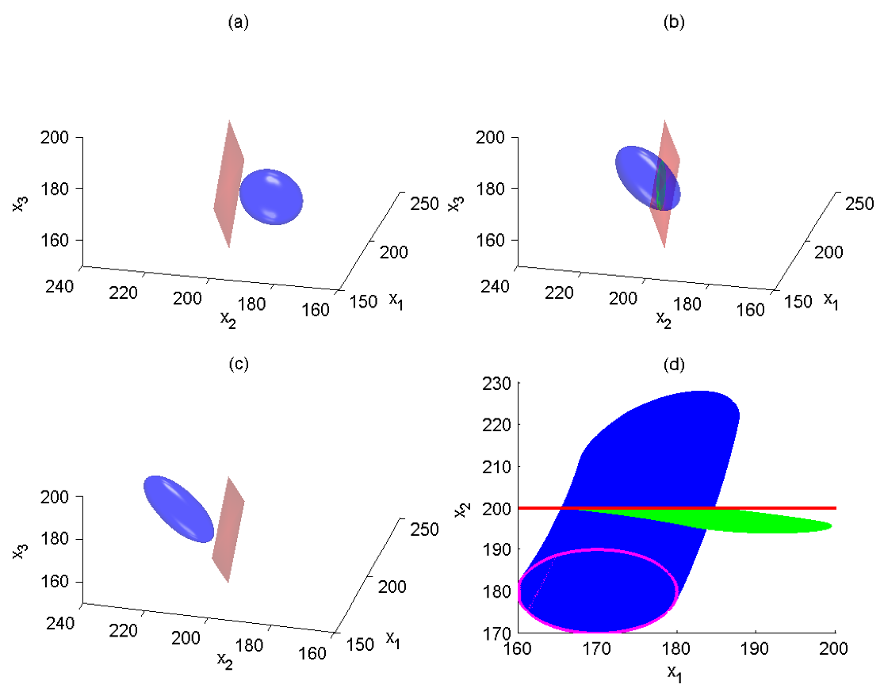
\includegraphics{hwreach.png}
\caption{Reach set of the free-flow system is blue, reach set of the congested
system is green, the guard is red.
(a) Reach set of the free-flow system at $t = 10$, before reaching the guard
(projection onto $(x_1,x_2,x_3)$).
(b) Reach set of the free-flow system at $t = 50$, crossing the guard.
(projection onto $(x_1,x_2,x_3)$).
(c) Reach set of the free-flow system at $t = 80$, after the guard is crossed.
(projection onto $(x_1,x_2,x_3)$).
(d) Reach set trace from $t=0$ to \emph{t=100}, free-flow system in blue,
congested system in green; bounds of initial conditions are marked with magenta
(projection onto $(x_1,x_2)$).}\label{chap_examples:hwreachfig}\end{figure}

Analyzing the values in array dVec, we conclude that the free-flow reach
set has nonempty intersection with hyperplane grdHyp at $t=18$ for
the first time, and at $t=68$ for the last time. Between
$t=18$ and $t=68$ it crosses the guard. \hyperref[chap_examples:hwreachfig]{Figure  \ref*{chap_examples:hwreachfig}} (a)
shows the free-flow reach set projection onto
$(x_1,x_2,x_3)$ subspace for $t=10$, before the guard
crossing; \hyperref[chap_examples:hwreachfig]{figure  \ref*{chap_examples:hwreachfig}} (b) for $t=50$, during the guard
crossing; and \hyperref[chap_examples:hwreachfig]{figure  \ref*{chap_examples:hwreachfig}} (c) for $t=80$, after the guard
was crossed.

For each time step that the intersection of the free-flow reach set and
the guard is nonempty, we establish a new initial time and a set of
initial conditions for the reach set computation according to dynamics
\eqref{chap_examples-cflow}. The initial time is the array index minus one, and the set of
initial conditions is the intersection of the free-flow reach set with
the guard.

\begin{Verbatim}[commandchars=\\\{\},numbers=left,firstnumber=1,stepnumber=1]
\PYG{n}{crsObjVec} \PYG{o}{=} \PYG{p}{[}\PYG{p}{]}\PYG{p}{;}
\PYG{k}{for} \PYG{n}{iInd} \PYG{o}{=} \PYG{l+m+mi}{1}\PYG{o}{:}\PYG{n}{size}\PYG{p}{(}\PYG{n}{indNonEmptyVec}\PYG{p}{,} \PYG{l+m+mi}{2}\PYG{p}{)}
    \PYG{n}{curTimeLimVec}\PYG{o}{=}\PYG{p}{[}\PYG{n}{indNonEmptyVec}\PYG{p}{(}\PYG{n}{iInd}\PYG{p}{)}\PYG{o}{\PYGZhy{}}\PYG{l+m+mi}{1} \PYG{n}{nSteps}\PYG{p}{]}\PYG{p}{;}
     \PYG{n}{rsObj} \PYG{o}{=} \PYG{n}{elltool}\PYG{p}{.}\PYG{n}{reach}\PYG{p}{.}\PYG{n}{ReachDiscrete}\PYG{p}{(}\PYG{n}{secSys}\PYG{p}{,}\PYG{p}{.}\PYG{p}{.}\PYG{p}{.}
         \PYG{n}{intersectEllVec}\PYG{p}{(}\PYG{n}{indNonEmptyVec}\PYG{p}{(}\PYG{n}{iInd}\PYG{p}{)}\PYG{p}{)}\PYG{p}{,} \PYG{p}{.}\PYG{p}{.}\PYG{p}{.}
             \PYG{n}{dirsMat}\PYG{p}{,} \PYG{n}{curTimeLimVec}\PYG{p}{,}\PYG{err}{\PYGZsq{}}\PYG{n}{isRegEnabled}\PYG{err}{\PYGZsq{}}\PYG{p}{,}\PYG{n+nb}{true}\PYG{p}{)}\PYG{p}{;}
     \PYG{n}{crsObjVec} \PYG{o}{=} \PYG{p}{[}\PYG{n}{crsObjVec} \PYG{n}{rsObj}\PYG{p}{]}\PYG{p}{;}
\PYG{n}{end}
\end{Verbatim}

The union of reach sets in array crs forms the reach set for the
congested dynamics.

A summary of the reach set computation of the linear hybrid system
\eqref{chap_examples-fflow}-\eqref{chap_examples-cflow} for $N=100$ time steps with one guard crossing
is given in \hyperref[chap_examples:hwreachfig]{figure  \ref*{chap_examples:hwreachfig}} (d), which shows the projection of the
reach set trace onto $(x_1,x_2)$ subspace. The system starts
evolving in time in free-flow mode from a set of initial conditions at
$t=0$, whose boundary is shown in magenta. The free-flow reach set
evolving from $t=0$ to $t=100$ is shown in blue. Between
$t=18$ and $t=68$ the free-flow reach set crosses the guard.
The guard is shown in red. For each nonempty intersection of the
free-flow reach set and the guard, the congested mode reach set starts
evolving in time until $t=100$. All the congested mode reach sets
are shown in green. Observe that in the congested mode, the density
$x_2$ in the congested part decreases slightly, while the density
$x_1$ upstream of the congested part increases. The blue set above
the guard is not actually reached, because the state evolves according
to the green region.

“Multi-Parametric Toolbox Homepage.” control.ee.ethz.ch/\textbackslash{}\textasciitilde{}mpt.

L.Muñoz, X.Sun, R.Horowitz, and L.Alvarez. 2003. “Traffic Density
Estimation with the Cell Transmission Model.” In \emph{Proceedings of the
American Control Conference}, 3750–3755. Denver, Colorado, USA.


\chapter{Summary and Outlook}
\label{chap_summary::doc}\label{chap_summary:summary-and-outlook}
Although some of the operations with ellipsoids are present in the
commercial Geometric Bounding Toolbox Veres et al. (2001; “Geometric
Bounding Toolbox Homepage”), the ellipsoid-related functionality of that
toolbox is rather limited.

\emph{Ellipsoidal Toolbox} is the first free MATLAB package that implements
ellipsoidal calculus and uses ellipsoidal methods for reachability
analysis of continuous- and discrete-time affine systems,
continuous-time linear systems with disturbances and switched systems,
whose dynamics changes at known times. The reach set computation for
hybrid systems whose guards are hyperplanes or polyhedra is not
implemented explicitly, but the tool for such computation exists,
namely, the operations of intersection of ellipsoid with hyperplane and
ellipsoid with halfspace.

“Geometric Bounding Toolbox Homepage.” www.sysbrain.com/gbt.

Veres, S. M., A. V. Kuntsevich, I. V. Vályi, S. Hermsmeyer, and D. S.
Wall. 2001. “Geometric Bounding Toolbox for MATLAB.” \emph{MATLAB/Simulink
Connections Catalogue}.


\chapter{Acknowledgement}
\label{chap_acknowledge::doc}\label{chap_acknowledge:acknowledgement}
The authors would like to thank Alexander B. Kurzhanski, Manfred Morari,
Johan Löfberg, Michal Kvasnica and Goran Frehse for their support of
this work by useful advice and encouragement.


\chapter{Function Reference}
\label{chap_func::doc}\label{chap_func:function-reference}

\section{ellipsoid}
\label{chap_func:ellipsoid}
\begin{Verbatim}[commandchars=\\\{\}]
CALCGRID - computes grid of 2d or 3d sphere and vertices for each face
           in the grid with number of points taken from ellObj
           nPlot2dPoints or nPlot3dPoints parameters
\end{Verbatim}

\begin{Verbatim}[commandchars=\\\{\}]
CHECKISME - determine whether input object is ellipsoid. And display
            message and abort function if input object
            is not ellipsoid

Input:
  regular:
      someObjArr: any[] - any type array of objects.

Example:
  ellObj = ellipsoid([1; 2], eye(2));
  ellipsoid.checkIsMe(ellObj)
\end{Verbatim}

\begin{Verbatim}[commandchars=\\\{\}]
Ellipsoid library of the Ellipsoidal Toolbox.


Constructor and data accessing functions:
-----------------------------------------
 ellipsoid    - Constructor of ellipsoid object.
 double       - Returns parameters of ellipsoid, i.e. center and shape
                matrix.
 parameters   - Same function as 'double'(legacy matter).
 dimension    - Returns dimension of ellipsoid and its rank.
 isdegenerate - Checks if ellipsoid is degenerate.
 isempty      - Checks if ellipsoid is empty.
 maxeig       - Returns the biggest eigenvalue of the ellipsoid.
 mineig       - Returns the smallest eigenvalue of the ellipsoid.
 trace        - Returns the trace of the ellipsoid.
 volume       - Returns the volume of the ellipsoid.


Overloaded operators and functions:
-----------------------------------
 eq      - Checks if two ellipsoids are equal.
 ne      - The opposite of 'eq'.
 gt, ge  - E1 \textgreater{} E2 (E1 \textgreater{}= E2) checks if, given the same center ellipsoid
           E1 contains E2.
 lt, le  - E1 \textless{} E2 (E1 \textless{}= E2) checks if, given the same center ellipsoid
           E2 contains E1.
 mtimes  - Given matrix A in R\textasciicircum{}(mxn) and ellipsoid E in R\textasciicircum{}n, returns
           (A * E).
 plus    - Given vector b in R\textasciicircum{}n and ellipsoid E in R\textasciicircum{}n, returns (E + b).
 minus   - Given vector b in R\textasciicircum{}n and ellipsoid E in R\textasciicircum{}n, returns (E - b).
 uminus  - Changes the sign of the center of ellipsoid.
 display - Displays the details about given ellipsoid object.
 inv     - inverts the shape matrix of the ellipsoid.
 plot    - Plots ellipsoid in 1D, 2D and 3D.


Geometry functions:
-------------------
 move2origin        - Moves the center of ellipsoid to the origin.
 shape              - Same as 'mtimes', but modifies only shape matrix of
                      the ellipsoid leaving its center as is.
 rho                - Computes the value of support function and
                      corresponding boundary point of the ellipsoid in
                      the given direction.
 polar              - Computes the polar ellipsoid to an ellipsoid that
                      contains the origin.
 projection         - Projects the ellipsoid onto a subspace specified
                      by  orthogonal basis vectors.
 minksum            - Computes and plots the geometric (Minkowski) sum of
                      given ellipsoids in 1D, 2D and 3D.
 minksum\_ea         - Computes the external ellipsoidal approximation of
                      geometric sum of given ellipsoids in given
                      direction.
 minksum\_ia         - Computes the internal ellipsoidal approximation of
                      geometric sum of given ellipsoids in given
                      direction.
 minkdiff           - Computes and plots the geometric (Minkowski)
                      difference of given ellipsoids in 1D, 2D and 3D.
 minkdiff\_ea        - Computes the external ellipsoidal approximation of
                      geometric difference of two ellipsoids in given
                      direction.
 minkdiff\_ia        - Computes the internal ellipsoidal approximation of
                      geometric difference of two ellipsoids in given
                      direction
 minkpm             - Computes and plots the geometric (Minkowski)
                      difference of a geometric sum of ellipsoids and a
                      single ellipsoid in 1D, 2D and 3D.
 minkpm\_ea          - Computes the external ellipsoidal approximation of
                      the geometric difference of a geometric sum of
                      ellipsoids and a single ellipsoid in given
                      direction.
 minkpm\_ia          - Computes the internal ellipsoidal approximation of
                      the geometric difference of a geometric sum of
                      ellipsoids and a single ellipsoid in given
                      direction.
 minkmp             - Computes and plots the geometric (Minkowski) sum of
                      a geometric difference of two single ellipsoids and
                      a geometric sum of ellipsoids in 1D, 2D and 3D.
 minkmp\_ea          - Computes the external ellipsoidal approximation of
                      the geometric sum of a geometric difference of two
                      single ellipsoids and a geometric sum of ellipsoids
                      in given direction.
 minkmp\_ia          -  Computes the internal ellipsoidal approximation of
                      the geometric sum of a geometric difference of
                      two single ellipsoids and a geometric sum of ellipsoids
                      in given direction.
 isbaddirection     - Checks if ellipsoidal approximation of geometric difference
                      of two ellipsoids in the given direction can be computed.
 doesIntersectionContain           - Checks if the union or intersection of
                      ellipsoids or polytopes lies inside the intersection
                      of given ellipsoids.
 isinternal         - Checks if given vector belongs to the union or intersection
                      of given ellipsoids.
 distance           - Computes the distance from ellipsoid to given point,
                      ellipsoid, hyperplane or polytope.
 intersect          - Checks if the union or intersection of ellipsoids intersects
                      with given ellipsoid, hyperplane, or polytope.
 intersection\_ea    - Computes the minimal volume ellipsoid containing intersection
                      of two ellipsoids, ellipsoid and halfspace, or ellipsoid
                      and polytope.
 intersection\_ia    - Computes the maximal ellipsoid contained inside the
                      intersection of two ellipsoids, ellipsoid and halfspace
                      or ellipsoid and polytope.
 ellintersection\_ia - Computes maximum volume ellipsoid that is contained
                      in the intersection of given ellipsoids (can be more than 2).
 ellunion\_ea        - Computes minimum volume ellipsoid that contains
                      the union of given ellipsoids.
 hpintersection     - Computes the intersection of ellipsoid with hyperplane.
\end{Verbatim}

\begin{Verbatim}[commandchars=\\\{\}]
DIMENSION - returns the dimension of the space in which the ellipsoid is
            defined and the actual dimension of the ellipsoid.

Input:
  regular:
    myEllArr: ellipsoid[nDims1,nDims2,...,nDimsN] - array of ellipsoids.

Output:
  regular:
    dimArr: double[nDims1,nDims2,...,nDimsN] - space dimensions.

  optional:
    rankArr: double[nDims1,nDims2,...,nDimsN] - dimensions of the
           ellipsoids in myEllArr.

Example:
  firstEllObj = ellipsoid();
  tempMatObj = [3 1; 0 1; -2 1];
  secEllObj = ellipsoid([1; -1; 1], tempMatObj*tempMatObj');
  thirdEllObj = ellipsoid(eye(2));
  fourthEllObj = ellipsoid(0);
  ellMat = [firstEllObj secEllObj; thirdEllObj fourthEllObj];
  [dimMat, rankMat] = ellMat.dimension()

  dimMat =

     0     3
     2     1

  rankMat =

     0     2
     2     0
\end{Verbatim}

\begin{Verbatim}[commandchars=\\\{\}]
DISP - Displays ellipsoid object.

Input:
  regular:
    myEllMat: ellipsoid [mRows, nCols] - matrix of ellipsoids.

Example:
  ellObj = ellipsoid([-2; -1], [2 -1; -1 1]);
  disp(ellObj)

  Ellipsoid with parameters
  Center:
      -2
      -1

  Shape Matrix:
       2    -1
      -1     1
\end{Verbatim}

\begin{Verbatim}[commandchars=\\\{\}]
DISPLAY - Displays the details of the ellipsoid object.

Input:
  regular:
      myEllMat: ellipsoid [mRows, nCols] - matrix of ellipsoids.

Example:
  ellObj = ellipsoid([-2; -1], [2 -1; -1 1]);
  display(ellObj)

  ellObj =

  Center:
      -2
      -1

  Shape Matrix:
       2    -1
      -1     1

  Nondegenerate ellipsoid in R\textasciicircum{}2.
\end{Verbatim}

\begin{Verbatim}[commandchars=\\\{\}]
DISTANCE - computes distance between the given ellipsoid (or array of
           ellipsoids) to the specified object (or arrays of objects):
           vector, ellipsoid, hyperplane or polytope.

Input:
  regular:
      ellObjArr: ellipsoid [nDims1, nDims2,..., nDimsN] -  array of
         ellipsoids of the same dimension.
      objArray: double / ellipsoid / hyperplane / polytope [nDims1,
          nDims2,..., nDimsN] - array of vectors or ellipsoids or
          hyperplanes or polytopes. If number of elements in objArray
          is more than 1, then it must be equal to the number of elements
          in ellObjArr.

  optional:
      isFlagOn: logical[1,1] - if true then distance is  computed in
          ellipsoidal metric, if false - in Euclidean metric (by default
          isFlagOn=false).

Output:
  regular:
    distValArray: double [nDims1, nDims2,..., nDimsN] - array of pairwise
          calculated distances.
          Negative distance value means
              for ellipsoid and vector: vector belongs to the ellipsoid,
              for ellipsoid and hyperplane: ellipsoid intersects the
                  hyperplane.
              Zero distance value means for ellipsoid and vector: vector
                  is aboundary point of the ellipsoid,
              for ellipsoid and hyperplane: ellipsoid  touches the
                  hyperplane.
  optional:
      statusArray: double [nDims1, nDims2,..., nDimsN] - array of time of
          computation of ellipsoids-vectors or ellipsoids-ellipsoids
          distances, or status of cvx solver for ellipsoids-polytopes
          distances.

Literature:
 1. Lin, A. and Han, S. On the Distance between Two Ellipsoids.
    SIAM Journal on Optimization, 2002, Vol. 13, No. 1 : pp. 298-308
 2. Stanley Chan, "Numerical method for Finding Minimum Distance to an
    Ellipsoid".
    http://videoprocessing.ucsd.edu/\textasciitilde{}stanleychan/publication/...
    unpublished/Ellipse.pdf

Example:
  ellObj = ellipsoid([-2; -1], [4 -1; -1 1]);
  tempMat = [1 1; 1 -1; -1 1; -1 -1]';
  distVec = ellObj.distance(tempMat)

  distVec =

       2.3428    1.0855    1.3799    -1.0000
\end{Verbatim}

\begin{Verbatim}[commandchars=\\\{\}]
DOESCONTAIN - checks if one ellipsoid contains the other ellipsoid or
              polytope. The condition for E1 = firstEllArr to contain
              E2 = secondEllArr is
              min(rho(l \textbar{} E1) - rho(l \textbar{} E2)) \textgreater{} 0, subject to \textless{}l, l\textgreater{} = 1.
              How checked if ellipsoid contains polytope is explained in
              doesContainPoly.
Input:
  regular:
      firstEllArr: ellipsoid [nDims1,nDims2,...,nDimsN]/[1,1] - first
          array of ellipsoids.
      secondObjArr: ellipsoid [nDims1,nDims2,...,nDimsN]/
          polytope[nDims1,nDims2,...,nDimsN]/[1,1] - array of the same
          size as firstEllArr or single ellipsoid or polytope.

   properties:
      mode: char[1, 1] - 'u' or 'i', go to description.
      computeMode: char[1,] - 'highDimFast' or 'lowDimFast'. Determines,
          which way function is computed, when secObjArr is polytope. If
          secObjArr is ellipsoid computeMode is ignored. 'highDimFast'
          works  faster for  high dimensions, 'lowDimFast' for low. If
          this property is omitted if dimension of ellipsoids is greater
          then 10, then 'hightDimFast' is choosen, otherwise -
          'lowDimFast'

Output:
  isPosArr: logical[nDims1,nDims2,...,nDimsN],
      resArr(iCount) = true - firstEllArr(iCount)
      contains secondObjArr(iCount), false - otherwise.

Example:
  firstEllObj = ellipsoid([-2; -1], [2 -1; -1 1]);
  secEllObj = ellipsoid([-1;0], eye(2));
  doesContain(firstEllObj,secEllObj)

  ans =

       0
\end{Verbatim}

\begin{Verbatim}[commandchars=\\\{\}]
DOESINTERSECTIONCONTAIN - checks if the intersection of ellipsoids
                          contains the union or intersection of given
                          ellipsoids or polytopes.

  res = DOESINTERSECTIONCONTAIN(fstEllArr, secEllArr, mode)
      Checks if the union
      (mode = 'u') or intersection (mode = 'i') of ellipsoids in
      secEllArr lies inside the intersection of ellipsoids in
      fstEllArr. Ellipsoids in fstEllArr and secEllArr must be
      of the same dimension. mode = 'u' (default) - union of
      ellipsoids in secEllArr. mode = 'i' - intersection.
  res = DOESINTERSECTIONCONTAIN(fstEllArr, secPolyArr, mode)
       Checks if the union
      (mode = 'u') or intersection (mode = 'i')  of polytopes in
      secPolyArr lies inside the intersection of ellipsoids in
      fstEllArr. Ellipsoids in fstEllArr and polytopes in secPolyArr
      must be of the same dimension. mode = 'u' (default) - union of
      polytopes in secPolyMat. mode = 'i' - intersection.

  To check if the union of ellipsoids secEllArr belongs to the
  intersection of ellipsoids fstEllArr, it is enough to check that
  every ellipsoid of secEllMat is contained in every
  ellipsoid of fstEllArr.
  Checking if the intersection of ellipsoids in secEllMat is inside
  intersection fstEllMat can be formulated as quadratically
  constrained quadratic programming (QCQP) problem.

  Let fstEllArr(iEll) = E(q, Q) be an ellipsoid with center q and shape
  matrix Q. To check if this ellipsoid contains the intersection of
  ellipsoids in secObjArr:
  E(q1, Q1), E(q2, Q2), ..., E(qn, Qn), we define the QCQP problem:
                    J(x) = \textless{}(x - q), Q\textasciicircum{}(-1)(x - q)\textgreater{} --\textgreater{} max
  with constraints:
                    \textless{}(x - q1), Q1\textasciicircum{}(-1)(x - q1)\textgreater{} \textless{}= 1   (1)
                    \textless{}(x - q2), Q2\textasciicircum{}(-1)(x - q2)\textgreater{} \textless{}= 1   (2)
                    ................................
                    \textless{}(x - qn), Qn\textasciicircum{}(-1)(x - qn)\textgreater{} \textless{}= 1   (n)

  If this problem is feasible, i.e. inequalities (1)-(n) do not
  contradict, or, in other words, intersection of ellipsoids
  E(q1, Q1), E(q2, Q2), ..., E(qn, Qn) is nonempty, then we can find
  vector y such that it satisfies inequalities (1)-(n)
  and maximizes function J. If J(y) \textless{}= 1, then ellipsoid E(q, Q)
  contains the given intersection, otherwise, it does not.

  The intersection of polytopes is a polytope, which is computed
  by the standard routine of MPT. How checked if intersection of
  ellipsoids contains polytope is explained in doesContainPoly.

  Checking if the union of polytopes belongs to the intersection
  of ellipsoids is the same as checking if its convex hull belongs
  to this intersection.

Input:
  regular:
      fstEllArr: ellipsoid [nDims1,nDims2,...,nDimsN] - array of ellipsoids
          of the same size.
      secEllArr: ellipsoid /
          polytope [nDims1,nDims2,...,nDimsN] - array of ellipsoids or
          polytopes of the same sizes.

          note: if mode == 'i', then fstEllArr, secEllVec should be
              array.

  properties:
      mode: char[1, 1] - 'u' or 'i', go to description.
      computeMode: char[1,] - 'highDimFast' or 'lowDimFast'. Determines,
          which way function is computed, when secObjArr is polytope. If
          secObjArr is ellipsoid computeMode is ignored. 'highDimFast'
          works  faster for  high dimensions, 'lowDimFast' for low. If
          this property is omitted if dimension of ellipsoids is greater
          then 10, then 'hightDimFast' is choosen, otherwise -
          'lowDimFast'


Output:
  res: double[1, 1] - result:
      -1 - problem is infeasible, for example, if s = 'i',
          but the intersection of ellipsoids in E2 is an empty set;
      0 - intersection is empty;
      1 - if intersection is nonempty.
  status: double[0, 0]/double[1, 1] - status variable. status is empty
      if mode == 'u' or mSecRows == nSecCols == 1.

Example:
  firstEllObj = [0 ; 0] + ellipsoid(eye(2, 2));
  secEllObj = [0 ; 0] + ellipsoid(2*eye(2, 2));
  thirdEllObj = [1; 0] + ellipsoid(0.5 * eye(2, 2));
  secEllObj.doesIntersectionContain([firstEllObj secEllObj], 'i')

  ans =

       1
\end{Verbatim}

\begin{Verbatim}[commandchars=\\\{\}]
DOUBLE - returns parameters of the ellipsoid.

Input:
  regular:
      myEll: ellipsoid [1, 1] - single ellipsoid of dimention nDims.


Output:
  myEllCentVec: double[nDims, 1] - center of the ellipsoid myEll.

  myEllShMat: double[nDims, nDims] - shape matrix of the ellipsoid myEll.

Example:
  ellObj = ellipsoid([-2; -1], [2 -1; -1 1]);
  [centVec, shapeMat] = double(ellObj)
  centVec =

      -2
      -1


  shapeMat =

       2    -1
      -1     1
\end{Verbatim}

\begin{Verbatim}[commandchars=\\\{\}]
ELLBNDR\_2D - compute the boundary of 2D ellipsoid. Private method.

Input:
  regular:
      myEll: ellipsoid [1, 1]- ellipsoid of the dimention 2.
  optional:
      nPoints: number of boundary points

Output:
  regular:
      bpMat: double[nPoints,2] - boundary points of ellipsoid
  optional:
      fVec: double[1,nFaces] - indices of points in each face of
          bpMat graph
\end{Verbatim}

\begin{Verbatim}[commandchars=\\\{\}]
ELLBNDR\_3D - compute the boundary of 3D ellipsoid.

Input:
  regular:
      myEll: ellipsoid [1, 1]- ellipsoid of the dimention 3.

  optional:
      nPoints: number of boundary points

Output:
  regular:
      bpMat: double[nPoints,3] - boundary points of ellipsoid
  optional:
      fMat: double[nFaces,3] - indices of face verties in bpMat
\end{Verbatim}

\begin{Verbatim}[commandchars=\\\{\}]
ELLINTERSECTION\_IA - computes maximum volume ellipsoid that is contained
                     in the intersection of given ellipsoids.


Input:
  regular:
      inpEllArr: ellipsoid [nDims1,nDims2,...,nDimsN] - array of
          ellipsoids of the same dimentions.

Output:
  outEll: ellipsoid [1, 1] - resulting maximum volume ellipsoid.

Example:
  firstEllObj = ellipsoid([-1; 1], [2 0; 0 3]);
  secEllObj = ellipsoid([1 2], eye(2);
  ellVec = [firstEllObj secEllObj];
  resEllObj = ellintersection\_ia(ellVec)

  resEllObj =

  Center:
      0.1847
      1.6914

  Shape Matrix:
      0.0340   -0.0607
     -0.0607    0.1713

  Nondegenerate ellipsoid in R\textasciicircum{}2.
\end{Verbatim}

\begin{Verbatim}[commandchars=\\\{\}]
ELLIPSOID - constructor of the ellipsoid object.

  Ellipsoid E = \PYGZob{} x in R\textasciicircum{}n : \textless{}(x - q), Q\textasciicircum{}(-1)(x - q)\textgreater{} \textless{}= 1 \PYGZcb{}, with current
      "Properties". Here q is a vector in R\textasciicircum{}n, and Q in R\textasciicircum{}(nxn) is positive
      semi-definite matrix

  ell = ELLIPSOID - Creates an empty ellipsoid

  ell = ELLIPSOID(shMat) - creates an ellipsoid with shape matrix shMat,
      centered at 0

   ell = ELLIPSOID(centVec, shMat) - creates an ellipsoid with shape matrix
      shMat and center centVec

  ell = ELLIPSOID(centVec, shMat, 'propName1', propVal1,...,
      'propNameN',propValN) - creates an ellipsoid with shape
      matrix shMat, center centVec and propName1 = propVal1,...,
      propNameN = propValN. In other cases "Properties"
      are taken from current values stored in
      elltool.conf.Properties.
  ellMat = Ellipsoid(centVecArray, shMatArray,
      ['propName1', propVal1,...,'propNameN',propValN]) -
      creates an array (possibly multidimensional) of
      ellipsoids with centers centVecArray(:,dim1,...,dimn)
      and matrices shMatArray(:,:,dim1,...dimn) with
      properties if given.

  These parameters can be accessed by DOUBLE(E) function call.
  Also, DIMENSION(E) function call returns the dimension of
  the space in which ellipsoid E is defined and the actual
  dimension of the ellipsoid; function ISEMPTY(E) checks if
  ellipsoid E is empty; function ISDEGENERATE(E) checks if
  ellipsoid E is degenerate.

Input:
  Case1:
    regular:
      shMatArray: double [nDim, nDim] /
          double [nDim, nDim, nDim1,...,nDimn] -
          shape matrices array

  Case2:
    regular:
      centVecArray: double [nDim,1] /
          double [nDim, 1, nDim1,...,nDimn] -
          centers array
      shMatArray: double [nDim, nDim] /
          double [nDim, nDim, nDim1,...,nDimn] -
          shape matrices array


  properties:
      absTol: double [1,1] - absolute tolerance with default value 10\textasciicircum{}(-7)
      relTol: double [1,1] - relative tolerance with default value 10\textasciicircum{}(-5)
      nPlot2dPoints: double [1,1] - number of points for 2D plot with
          default value 200
      nPlot3dPoints: double [1,1] - number of points for 3D plot with
           default value 200.

Output:
  ellMat: ellipsoid [1,1] / ellipsoid [nDim1,...nDimn] -
      ellipsoid with specified properties
      or multidimensional array of ellipsoids.

Example:
  ellObj = ellipsoid([1 0 -1 6]', 9*eye(4));
\end{Verbatim}

\begin{Verbatim}[commandchars=\\\{\}]
ELLUNION\_EA - computes minimum volume ellipsoid that contains union
              of given ellipsoids.

Input:
  regular:
      inpEllMat: ellipsoid [nDims1,nDims2,...,nDimsN] - array of
          ellipsoids of the same dimentions.

Output:
  outEll: ellipsoid [1, 1] - resulting minimum volume ellipsoid.

Example:
  firstEllObj = ellipsoid([-1; 1], [2 0; 0 3]);
  secEllObj = ellipsoid([1 2], eye(2));
  ellVec = [firstEllObj secEllObj];
  resEllObj = ellunion\_ea(ellVec)
  resEllObj =

  Center:
     -0.3188
      1.2936

  Shape Matrix:
      5.4573    1.3386
      1.3386    4.1037

  Nondegenerate ellipsoid in R\textasciicircum{}2.
\end{Verbatim}

\begin{Verbatim}[commandchars=\\\{\}]
FROMREPMAT - returns array of equal ellipsoids the same
             size as stated in sizeVec argument

  ellArr = fromRepMat(sizeVec) - creates an array  size
           sizeVec of empty ellipsoids.

  ellArr = fromRepMat(shMat,sizeVec) - creates an array
           size sizeVec of ellipsoids with shape matrix
           shMat.

  ellArr = fromRepMat(cVec,shMat,sizeVec) - creates an
           array size sizeVec of ellipsoids with shape
           matrix shMat and center cVec.

Input:
  Case1:
      regular:
          sizeVec: double[1,n] - vector of size, have
          integer values.

  Case2:
      regular:
          shMat: double[nDim, nDim] - shape matrix of
          ellipsoids.
          sizeVec: double[1,n] - vector of size, have
          integer values.

  Case3:
      regular:
          cVec: double[nDim,1] - center vector of
          ellipsoids
          shMat: double[nDim, nDim] - shape matrix of
          ellipsoids.
          sizeVec: double[1,n] - vector of size, have
          integer values.

  properties:
      absTol: double [1,1] - absolute tolerance with default
          value 10\textasciicircum{}(-7)
      relTol: double [1,1] - relative tolerance with default
          value 10\textasciicircum{}(-5)
      nPlot2dPoints: double [1,1] - number of points for 2D plot
          with default value 200
      nPlot3dPoints: double [1,1] - number of points for 3D plot
          with default value 200.
\end{Verbatim}

\begin{Verbatim}[commandchars=\\\{\}]
fromStruct -- converts structure array into ellipsoid array.

Input:
  regular:
      SEllArr: struct [nDim1, nDim2, ...] - array
          of structures with the following fields:

      q: double[1, nEllDim] - the center of ellipsoid
      Q: double[nEllDim, nEllDim] - the shape matrix of ellipsoid
Output:
      ellArr: ellipsoid [nDim1, nDim2, ...] - ellipsoid array with size of
          SEllArr.

Example:
s = struct('Q', eye(2), 'q', [0 0]);
ellipsoid.fromStruct(s)

-------ellipsoid object-------
Properties:
   \textbar{}
   \textbar{}-- actualClass : 'ellipsoid'
   \textbar{}--------- size : [1, 1]

Fields (name, type, description):
    'Q'    'double'    'Configuration matrix'
    'q'    'double'    'Center'

Data:
   \textbar{}
   \textbar{}-- q : [0 0]
   \textbar{}       -----
   \textbar{}-- Q : \textbar{}1\textbar{}0\textbar{}
   \textbar{}       \textbar{}0\textbar{}1\textbar{}
   \textbar{}       -----
\end{Verbatim}

\begin{Verbatim}[commandchars=\\\{\}]
GETABSTOL - gives the array of absTol for all elements in ellArr

Input:
  regular:
      ellArr: ellipsoid[nDim1, nDim2, ...] - multidimension array
          of ellipsoids
  optional
      fAbsTolFun: function\_handle[1,1] - function that apply
          to the absTolArr. The default is @min.

Output:
  regular:
      absTolArr: double [absTol1, absTol2, ...] - return absTol for
          each element in ellArr
  optional:
      absTol: double[1,1] - return result of work fAbsTolFun with
          the absTolArr

Usage:
  use [\textasciitilde{},absTol] = ellArr.getAbsTol() if you want get only
      absTol,
  use [absTolArr,absTol] = ellArr.getAbsTol() if you want get
      absTolArr and absTol,
  use absTolArr = ellArr.getAbsTol() if you want get only absTolArr

Example:
  firstEllObj = ellipsoid([-1; 1], [2 0; 0 3]);
  secEllObj = ellipsoid([1 2], eye(2));
  ellVec = [firstEllObj secEllObj];
  absTolVec = ellVec.getAbsTol()

  absTolVec =

     1.0e-07 *

      1.0000    1.0000
\end{Verbatim}

\begin{Verbatim}[commandchars=\\\{\}]
GETBOUNDARY - computes the boundary of an ellipsoid.

Input:
  regular:
      myEll: ellipsoid [1, 1]- ellipsoid of the dimention 2 or 3.
  optional:
      nPoints: number of boundary points

Output:
  regular:
      bpMat: double[nPoints,nDim] - boundary points of ellipsoid
  optional:
      fVec: double[1,nFaces]/double[nFacex,nDim] - indices of points in
          each face of bpMat graph
\end{Verbatim}

\begin{Verbatim}[commandchars=\\\{\}]
GETBOUNDARYBYFACTOR - computes grid of 2d or 3d ellipsoid and vertices
                      for each face in the grid
\end{Verbatim}

\begin{Verbatim}[commandchars=\\\{\}]
GETCENTERVEC - returns centerVec vector of given ellipsoid

Input:
  regular:
     self: ellipsoid[1,1]

Output:
  centerVecVec: double[nDims,1] - centerVec of ellipsoid

Example:
  ellObj = ellipsoid([1; 2], eye(2));
  getCenterVec(ellObj)

  ans =

       1
       2
\end{Verbatim}

\begin{Verbatim}[commandchars=\\\{\}]
GETCOPY - gives array the same size as ellArr with copies of elements of
          ellArr.

Input:
  regular:
      ellArr: ellipsoid[nDim1, nDim2,...] - multidimensional array of
          ellipsoids.

Output:
  copyEllArr: ellipsoid[nDim1, nDim2,...] - multidimension array of
      copies of elements of ellArr.

Example:
  firstEllObj = ellipsoid([-1; 1], [2 0; 0 3]);
  secEllObj = ellipsoid([1; 2], eye(2));
  ellVec = [firstEllObj secEllObj];
  copyEllVec = getCopy(ellVec)

  copyEllVec =
  1x2 array of ellipsoids.
\end{Verbatim}

\begin{Verbatim}[commandchars=\\\{\}]
GETINV - do the same as INV method: inverts shape matrices of ellipsoids
      in the given array, with only difference, that it doesn't modify
      input array of ellipsoids.

Input:
  regular:
    myEllArr: ellipsoid [nDims1,nDims2,...,nDimsN] - array of ellipsoids.

Output:
   invEllArr: ellipsoid [nDims1,nDims2,...,nDimsN] - array of ellipsoids
      with inverted shape matrices.

Example:
  ellObj = ellipsoid([1; 1], [4 -1; -1 5]);
  invEllObj = ellObj.getInv()

  invEllObj =

  Center:
       1
       1

  Shape Matrix:
      0.2632    0.0526
      0.0526    0.2105

  Nondegenerate ellipsoid in R\textasciicircum{}2.
\end{Verbatim}

\begin{Verbatim}[commandchars=\\\{\}]
GETMOVE2ORIGIN - do the same as MOVE2ORIGIN method: moves ellipsoids in
      the given array to the origin, with only difference, that it doesn't
      modify input array of ellipsoids.

Input:
  regular:
      inpEllArr: ellipsoid [nDims1,nDims2,...,nDimsN] - array of
          ellipsoids.

Output:
  outEllArr: ellipsoid [nDims1,nDims2,...,nDimsN] - array of ellipsoids
      with the same shapes as in inpEllArr centered at the origin.

Example:
  ellObj = ellipsoid([-2; -1], [4 -1; -1 1]);
  outEllObj = ellObj.getMove2Origin()

  outEllObj =

  Center:
       0
       0

  Shape:
       4    -1
      -1     1

  Nondegenerate ellipsoid in R\textasciicircum{}2.
\end{Verbatim}

\begin{Verbatim}[commandchars=\\\{\}]
GETNPLOT2DPOINTS - gives value of nPlot2dPoints property of ellipsoids
                   in ellArr

Input:
  regular:
      ellArr: ellipsoid[nDim1, nDim2,...] - mltidimensional array of
          ellipsoids

Output:
      nPlot2dPointsArr: double[nDim1, nDim2,...] - multidimension array
          of nPlot2dPoints property for ellipsoids in ellArr
Example:
  firstEllObj = ellipsoid([-1; 1], [2 0; 0 3]);
  secEllObj = ellipsoid([1 ;2], eye(2));
  ellVec = [firstEllObj secEllObj];
  ellVec.getNPlot2dPoints()

  ans =

     200   200
\end{Verbatim}

\begin{Verbatim}[commandchars=\\\{\}]
GETNPLOT3DPOINTS - gives value of nPlot3dPoints property of ellipsoids
                   in ellArr

Input:
  regular:
      ellArr: ellipsoid[nDim1, nDim2,...] - mltidimensional array  of
         ellipsoids

Output:
      nPlot2dPointsArr: double[nDim1, nDim2,...] - multidimension array
          of nPlot3dPoints property for ellipsoids in ellArr

Example:
  firstEllObj = ellipsoid([-1; 1], [2 0; 0 3]);
  secEllObj = ellipsoid([1 ;2], eye(2));
  ellVec = [firstEllObj secEllObj];
  ellVec.getNPlot3dPoints()

  ans =

     200   200
\end{Verbatim}

\begin{Verbatim}[commandchars=\\\{\}]
GETPROJECTION - do the same as PROJECTION method: computes projection of
      the ellipsoid onto the given subspace, with only difference, that
      it doesn't modify input array of ellipsoids.

Input:
  regular:
      ellArr: ellipsoid [nDims1,nDims2,...,nDimsN] - array
          of ellipsoids.
      basisMat: double[nDim, nSubSpDim] - matrix of orthogonal basis
          vectors

Output:
  projEllArr: ellipsoid [nDims1,nDims2,...,nDimsN] - array of
      projected ellipsoids, generally, of lower dimension.

Example:
  ellObj = ellipsoid([-2; -1; 4], [4 -1 0; -1 1 0; 0 0 9]);
  basisMat = [0 1 0; 0 0 1]';
  outEllObj = ellObj.getProjection(basisMat)

  outEllObj =

  Center:
      -1
       4

  Shape:
      1     0
      0     9

  Nondegenerate ellipsoid in R\textasciicircum{}2.
\end{Verbatim}

\begin{Verbatim}[commandchars=\\\{\}]
GETRELTOL - gives the array of relTol for all elements in ellArr

Input:
  regular:
      ellArr: ellipsoid[nDim1, nDim2, ...] - multidimension array
          of ellipsoids
  optional:
      fRelTolFun: function\_handle[1,1] - function that apply
          to the relTolArr. The default is @min.
Output:
  regular:
      relTolArr: double [relTol1, relTol2, ...] - return relTol for
          each element in ellArr
  optional:
      relTol: double[1,1] - return result of work fRelTolFun with
          the relTolArr

Usage:
  use [\textasciitilde{},relTol] = ellArr.getRelTol() if you want get only
      relTol,
  use [relTolArr,relTol] = ellArr.getRelTol() if you want get
      relTolArr and relTol,
  use relTolArr = ellArr.getRelTol() if you want get only relTolArr

Example:
  firstEllObj = ellipsoid([-1; 1], [2 0; 0 3]);
  secEllObj = ellipsoid([1 ;2], eye(2));
  ellVec = [firstEllObj secEllObj];
  ellVec.getRelTol()

  ans =

     1.0e-05 *

      1.0000    1.0000
\end{Verbatim}

\begin{Verbatim}[commandchars=\\\{\}]
GETSHAPE -  do the same as SHAPE method: modifies the shape matrix of the
   ellipsoid without changing its center, with only difference, that
   it doesn't modify input array of ellipsoids.

Input:
  regular:
      ellArr: ellipsoid [nDims1,nDims2,...,nDimsN] - array
          of ellipsoids.
      modMat: double[nDim, nDim]/[1,1] - square matrix or scalar

Output:
   outEllArr: ellipsoid [nDims1,nDims2,...,nDimsN] - array of modified
      ellipsoids.

Example:
  ellObj = ellipsoid([-2; -1], [4 -1; -1 1]);
  tempMat = [0 1; -1 0];
  outEllObj = ellObj.getShape(tempMat)

  outEllObj =

  Center:
      -2
      -1

  Shape:
      1     1
      1     4

  Nondegenerate ellipsoid in R\textasciicircum{}2.
\end{Verbatim}

\begin{Verbatim}[commandchars=\\\{\}]
GETSHAPEMAT - returns shapeMat matrix of given ellipsoid

Input:
  regular:
     self: ellipsoid[1,1]

Output:
  shMat: double[nDims,nDims] - shapeMat matrix of ellipsoid

Example:
  ellObj = ellipsoid([1; 2], eye(2));
  getShapeMat(ellObj)

  ans =

       1     0
       0     1
\end{Verbatim}

\begin{Verbatim}[commandchars=\\\{\}]
HPINTERSECTION - computes the intersection of ellipsoid with hyperplane.

Input:
  regular:
      myEllArr: ellipsoid [nDims1,nDims2,...,nDimsN]/[1,1] - array
          of ellipsoids.
      myHypArr: hyperplane [nDims1,nDims2,...,nDimsN]/[1,1] - array
          of hyperplanes of the same size.

Output:
  intEllArr: ellipsoid [nDims1,nDims2,...,nDimsN] - array of ellipsoids
      resulting from intersections.

  isnIntersectedArr: logical [nDims1,nDims2,...,nDimsN].
      isnIntersectedArr(iCount) = true, if myEllArr(iCount)
      doesn't intersect myHipArr(iCount),
      isnIntersectedArr(iCount) = false, otherwise.

Example:
  ellObj = ellipsoid([-2; -1], [4 -1; -1 1]);
  hypMat = [hyperplane([0 -1; -1 0]', 1); hyperplane([0 -2; -1 0]', 1)];
  ellMat = ellObj.hpintersection(hypMat)

  ellMat =
  2x2 array of ellipsoids.
\end{Verbatim}

\begin{Verbatim}[commandchars=\\\{\}]
INTERSECT - checks if the union or intersection of ellipsoids intersects
            given ellipsoid, hyperplane or polytope.

  resArr = INTERSECT(myEllArr, objArr, mode) - Checks if the union
      (mode = 'u') or intersection (mode = 'i') of ellipsoids
      in myEllArr intersects with objects in objArr.
      objArr can be array of ellipsoids, array of hyperplanes,
      or array of polytopes.
      Ellipsoids, hyperplanes or polytopes in objMat must have
      the same dimension as ellipsoids in myEllArr.
      mode = 'u' (default) - union of ellipsoids in myEllArr.
      mode = 'i' - intersection.

  If we need to check the intersection of union of ellipsoids in
  myEllArr (mode = 'u'), or if myEllMat is a single ellipsoid,
  it can be done by calling distance function for each of the
  ellipsoids in myEllArr and objMat, and if it returns negative value,
  the intersection is nonempty. Checking if the intersection of
  ellipsoids in myEllArr (with size of myEllMat greater than 1)
  intersects with ellipsoids or hyperplanes in objArr is more
  difficult. This problem can be formulated as quadratically
  constrained quadratic programming (QCQP) problem.

  Let objArr(iObj) = E(q, Q) be an ellipsoid with center q and shape
  matrix Q. To check if this ellipsoid intersects (or touches) the
  intersection of ellipsoids in meEllArr: E(q1, Q1), E(q2, Q2), ...,
  E(qn, Qn), we define the QCQP problem:
                    J(x) = \textless{}(x - q), Q\textasciicircum{}(-1)(x - q)\textgreater{} --\textgreater{} min
  with constraints:
                     \textless{}(x - q1), Q1\textasciicircum{}(-1)(x - q1)\textgreater{} \textless{}= 1   (1)
                     \textless{}(x - q2), Q2\textasciicircum{}(-1)(x - q2)\textgreater{} \textless{}= 1   (2)
                     ................................
                     \textless{}(x - qn), Qn\textasciicircum{}(-1)(x - qn)\textgreater{} \textless{}= 1   (n)

  If this problem is feasible, i.e. inequalities (1)-(n) do not
  contradict, or, in other words, intersection of ellipsoids
  E(q1, Q1), E(q2, Q2), ..., E(qn, Qn) is nonempty, then we can find
  vector y such that it satisfies inequalities (1)-(n) and minimizes
  function J. If J(y) \textless{}= 1, then ellipsoid E(q, Q) intersects or touches
  the given intersection, otherwise, it does not. To check if E(q, Q)
  intersects the union of E(q1, Q1), E(q2, Q2), ..., E(qn, Qn),
  we compute the distances from this ellipsoids to those in the union.
  If at least one such distance is negative,
  then E(q, Q) does intersect the union.

  If we check the intersection of ellipsoids with hyperplane
  objArr = H(v, c), it is enough to check the feasibility
  of the problem
                      1'x --\textgreater{} min
  with constraints (1)-(n), plus
                    \textless{}v, x\textgreater{} - c = 0.

  Checking the intersection of ellipsoids with polytope
  objArr = P(A, b) reduces to checking if there any x, satisfying
  constraints (1)-(n) and
                       Ax \textless{}= b.

Input:
  regular:
      myEllArr: ellipsoid [nDims1,nDims2,...,nDimsN] - array of
           ellipsoids.
      objArr: ellipsoid / hyperplane /
          / polytope [nDims1,nDims2,...,nDimsN] - array of ellipsoids or
          hyperplanes or polytopes of the same sizes.

  optional:
      mode: char[1, 1] - 'u' or 'i', go to description.

          note: If mode == 'u', then mRows, nCols should be equal to 1.

Output:
  resArr: double[nDims1,nDims2,...,nDimsN] - return:
      resArr(iCount) = -1 in case parameter mode is set
          to 'i' and the intersection of ellipsoids in myEllArr
          is empty.
      resArr(iCount) = 0 if the union or intersection of
          ellipsoids in myEllArr does not intersect the object
          in objArr(iCount).
      resArr(iCount) = 1 if the union or intersection of
          ellipsoids in myEllArr and the object in objArr(iCount)
          have nonempty intersection.
  statusArr: double[0, 0]/double[nDims1,nDims2,...,nDimsN] - status
      variable. statusArr is empty if mode = 'u'.

Example:
  firstEllObj = ellipsoid([-2; -1], [4 -1; -1 1]);
  secEllObj = firstEllObj + [5; 5];
  hypObj  = hyperplane([1; -1]);
  ellVec = [firstEllObj secEllObj];
  ellVec.intersect(hypObj)

  ans =

       1

  ellVec.intersect(hypObj, 'i')

  ans =

      -1
\end{Verbatim}

\begin{Verbatim}[commandchars=\\\{\}]
INTERSECTION\_EA - external ellipsoidal approximation of the
                  intersection of two ellipsoids, or ellipsoid and
                  halfspace, or ellipsoid and polytope.

  outEllArr = INTERSECTION\_EA(myEllArr, objArr) Given two ellipsoidal
      matrixes of equal sizes, myEllArr and objArr = ellArr, or,
      alternatively, myEllArr or ellMat must be a single ellipsoid,
      computes the ellipsoid that contains the intersection of two
      corresponding ellipsoids from myEllArr and from ellArr.
  outEllArr = INTERSECTION\_EA(myEllArr, objArr) Given matrix of
      ellipsoids myEllArr and matrix of hyperplanes objArr = hypArr
      whose sizes match, computes the external ellipsoidal
      approximations of intersections of ellipsoids
      and halfspaces defined by hyperplanes in hypArr.
      If v is normal vector of hyperplane and c - shift,
      then this hyperplane defines halfspace
              \textless{}v, x\textgreater{} \textless{}= c.
  outEllArr = INTERSECTION\_EA(myEllArr, objArr) Given matrix of
      ellipsoids myEllArr and matrix of polytopes objArr = polyArr
      whose sizes match, computes the external ellipsoidal
      approximations of intersections of ellipsoids myEllMat and
      polytopes polyArr.

  The method used to compute the minimal volume overapproximating
  ellipsoid is described in "Ellipsoidal Calculus Based on
  Propagation and Fusion" by Lluis Ros, Assumpta Sabater and
  Federico Thomas; IEEE Transactions on Systems, Man and Cybernetics,
  Vol.32, No.4, pp.430-442, 2002. For more information, visit
  http://www-iri.upc.es/people/ros/ellipsoids.html

  For polytopes this method won't give the minimal volume
  overapproximating ellipsoid, but just some overapproximating ellipsoid.

Input:
  regular:
      myEllArr: ellipsoid [nDims1,nDims2,...,nDimsN]/[1,1] - array
          of ellipsoids.
      objArr: ellipsoid / hyperplane /
          / polytope [nDims1,nDims2,...,nDimsN]/[1,1]  - array of
          ellipsoids or hyperplanes or polytopes of the same sizes.

Example:
  firstEllObj = ellipsoid([-2; -1], [4 -1; -1 1]);
  secEllObj = firstEllObj + [5; 5];
  ellVec = [firstEllObj secEllObj];
  thirdEllObj  = ell\_unitball(2);
  externalEllVec = ellVec.intersection\_ea(thirdEllObj)

  externalEllVec =
  1x2 array of ellipsoids.
\end{Verbatim}

\begin{Verbatim}[commandchars=\\\{\}]
INTERSECTION\_IA - internal ellipsoidal approximation of the
                  intersection of ellipsoid and ellipsoid,
                  or ellipsoid and halfspace, or ellipsoid
                  and polytope.

  outEllArr = INTERSECTION\_IA(myEllArr, objArr) - Given two
      ellipsoidal matrixes of equal sizes, myEllArr and
      objArr = ellArr, or, alternatively, myEllMat or ellMat must be
      a single ellipsoid, comuptes the internal ellipsoidal
      approximations of intersections of two corresponding ellipsoids
      from myEllMat and from ellMat.
  outEllArr = INTERSECTION\_IA(myEllArr, objArr) - Given matrix of
      ellipsoids myEllArr and matrix of hyperplanes objArr = hypArr
      whose sizes match, computes the internal ellipsoidal
      approximations of intersections of ellipsoids and halfspaces
      defined by hyperplanes in hypMat.
      If v is normal vector of hyperplane and c - shift,
      then this hyperplane defines halfspace
                 \textless{}v, x\textgreater{} \textless{}= c.
  outEllArr = INTERSECTION\_IA(myEllArr, objArr) - Given matrix of
      ellipsoids  myEllArr and matrix of polytopes objArr = polyArr
      whose sizes match, computes the internal ellipsoidal
      approximations of intersections of ellipsoids myEllArr
      and polytopes polyArr.

  The method used to compute the minimal volume overapproximating
  ellipsoid is described in "Ellipsoidal Calculus Based on
  Propagation and Fusion" by Lluis Ros, Assumpta Sabater and
  Federico Thomas; IEEE Transactions on Systems, Man and Cybernetics,
  Vol.32, No.4, pp.430-442, 2002. For more information, visit
  http://www-iri.upc.es/people/ros/ellipsoids.html

  The method used to compute maximum volume ellipsoid inscribed in
  intersection of ellipsoid and polytope, is modified version of
  algorithm of finding maximum volume ellipsoid inscribed in intersection
  of ellipsoids discribed in Stephen Boyd and Lieven Vandenberghe "Convex
  Optimization". It works properly for nondegenerate ellipsoid, but for
  degenerate ellipsoid result would not lie in this ellipsoid. The result
  considered as empty ellipsoid, when maximum absolute velue of element
  in its matrix is less than myEllipsoid.getAbsTol().

Input:
  regular:
      myEllArr: ellipsoid [nDims1,nDims2,...,nDimsN]/[1,1] - array
          of ellipsoids.
      objArr: ellipsoid / hyperplane /
          / polytope [nDims1,nDims2,...,nDimsN]/[1,1]  - array of
          ellipsoids or hyperplanes or polytopes of the same sizes.

Output:
   outEllArr: ellipsoid [nDims1,nDims2,...,nDimsN] - array of internal
      approximating ellipsoids; entries can be empty ellipsoids
      if the corresponding intersection is empty.

Example:
  firstEllObj = ellipsoid([-2; -1], [4 -1; -1 1]);
  secEllObj = firstEllObj + [5; 5];
  ellVec = [firstEllObj secEllObj];
  thirdEllObj  = ell\_unitball(2);
  internalEllVec = ellVec.intersection\_ia(thirdEllObj)

  internalEllVec =
  1x2 array of ellipsoids.
\end{Verbatim}

\begin{Verbatim}[commandchars=\\\{\}]
INV - inverts shape matrices of ellipsoids in the given array,
      modified given array is on output (not its copy).


  invEllArr = INV(myEllArr)  Inverts shape matrices of ellipsoids
      in the array myEllMat. In case shape matrix is sigular, it is
      regularized before inversion.

Input:
  regular:
    myEllArr: ellipsoid [nDims1,nDims2,...,nDimsN] - array of ellipsoids.

Output:
   myEllArr: ellipsoid [nDims1,nDims2,...,nDimsN] - array of ellipsoids
      with inverted shape matrices.

Example:
  ellObj = ellipsoid([1; 1], [4 -1; -1 5]);
  ellObj.inv()

  ans =

  Center:
       1
       1

  Shape Matrix:
      0.2632    0.0526
      0.0526    0.2105

  Nondegenerate ellipsoid in R\textasciicircum{}2.
\end{Verbatim}

\begin{Verbatim}[commandchars=\\\{\}]
ISEMPTY - checks if the ellipsoid object is empty.

Input:
  regular:
      myEllArr: ellipsoid [nDims1,nDims2,...,nDimsN] - array of
           ellipsoids.

Output:
  isPositiveArr: logical[nDims1,nDims2,...,nDimsN],
      isPositiveArr(iCount) = true - if ellipsoid
      myEllMat(iCount) is empty, false - otherwise.

Example:
  ellObj = ellipsoid();
  isempty(ellObj)

  ans =

       1
\end{Verbatim}

\begin{Verbatim}[commandchars=\\\{\}]
ISEQUAL - produces logical array the same size as
          ellFirstArr/ellFirstArr (if they have the same).
          isEqualArr[iDim1, iDim2,...] is true if corresponding
          ellipsoids are equal and false otherwise.

Input:
  regular:
      ellFirstArr: ellipsoid[nDim1, nDim2,...] - multidimensional array
          of ellipsoids.
      ellSecArr: ellipsoid[nDim1, nDim2,...] - multidimensional array
          of ellipsoids.
  properties:
      'isPropIncluded': makes to compare second value properties, such as
      absTol etc.
Output:
  isEqualArr: logical[nDim1, nDim2,...] - multidimension array of
      logical values. isEqualArr[iDim1, iDim2,...] is true if
      corresponding ellipsoids are equal and false otherwise.

  reportStr: char[1,] - comparison report.
\end{Verbatim}

\begin{Verbatim}[commandchars=\\\{\}]
ISINSIDE - checks if given ellipsoid(or array of
           ellipsoids) lies inside given object(or array
           of objects): ellipsoid or polytope.

Input:
  regular:
      ellArr: ellipsoid[nDims1,nDims2,...,nDimsN] - array
              of ellipsoids of the same dimension.
      objArr: ellipsoid/
              polytope[nDims1,nDims2,...,nDimsN] of
              objects of the same dimension. If
              ellArr and objArr both non-scalar, than
              size of ellArr must be the same as size of
              objArr. Note that polytopes could be
              combined only in vector of size [1,N].
Output:
  regular:
      resArr: logical[nDims1,nDims2,...,nDimsN] array of
              results. resArr[iDim1,...,iDimN] = true, if
              ellArr[iDim1,...,iDimN] lies inside
              objArr[iDim1,...,iDimN].

Example:
  firstEllObj = [0 ; 0] + ellipsoid(eye(2, 2));
  secEllObj = [0 ; 0] + ellipsoid(2*eye(2, 2));
  firstEllObj.isInside(secEllObj)

  ans =

       1
\end{Verbatim}

\begin{Verbatim}[commandchars=\\\{\}]
ISBADDIRECTION - checks if ellipsoidal approximations of geometric
                 difference of two ellipsoids can be computed for
                 given directions.
  isBadDirVec = ISBADDIRECTION(fstEll, secEll, dirsMat) - Checks if
      it is possible to build ellipsoidal approximation of the
      geometric difference of two ellipsoids fstEll - secEll in
      directions specified by matrix dirsMat (columns of dirsMat
      are direction vectors). Type 'help minkdiff\_ea' or
      'help minkdiff\_ia' for more information.

Input:
  regular:
      fstEll: ellipsoid [1, 1] - first ellipsoid. Suppose nDim - space
          dimension.
      secEll: ellipsoid [1, 1] - second ellipsoid of the same dimention.
      dirsMat: numeric[nDims, nCols] - matrix whose columns are
          direction vectors that need to be checked.
      absTol: double [1,1] - absolute tolerance

Output:
   isBadDirVec: logical[1, nCols] - array of true or false with length
      being equal to the number of columns in matrix dirsMat.
      ture marks direction vector as bad - ellipsoidal approximation
      true marks direction vector as bad - ellipsoidal approximation
      cannot be computed for this direction. false means the opposite.
\end{Verbatim}

\begin{Verbatim}[commandchars=\\\{\}]
ISBIGGER - checks if one ellipsoid would contain the other if their
           centers would coincide.

  isPositive = ISBIGGER(fstEll, secEll) - Given two single ellipsoids
      of the same dimension, fstEll and secEll, check if fstEll
      would contain secEll inside if they were both
      centered at origin.

Input:
  regular:
      fstEll: ellipsoid [1, 1] - first ellipsoid.
      secEll: ellipsoid [1, 1] - second ellipsoid
          of the same dimention.

Output:
  isPositive: logical[1, 1], true - if ellipsoid fstEll
      would contain secEll inside, false - otherwise.

Example:
  firstEllObj = ellipsoid([1; 1], eye(2));
  secEllObj = ellipsoid([1; 1], [4 -1; -1 5]);
  isbigger(firstEllObj, secEllObj)

  ans =

       0
\end{Verbatim}

\begin{Verbatim}[commandchars=\\\{\}]
ISDEGENERATE - checks if the ellipsoid is degenerate.

Input:
  regular:
      myEllArr: ellipsoid[nDims1,nDims2,...,nDimsN] - array of ellipsoids.

Output:
  isPositiveArr: logical[nDims1,nDims2,...,nDimsN],
      isPositiveArr(iCount) = true if ellipsoid myEllMat(iCount)
      is degenerate, false - otherwise.

Example:
  ellObj = ellipsoid([1; 1], eye(2));
  isdegenerate(ellObj)

  ans =

       0
\end{Verbatim}

\begin{Verbatim}[commandchars=\\\{\}]
ISINTERNAL - checks if given points belong to the union or intersection
             of ellipsoids in the given array.

  isPositiveVec = ISINTERNAL(myEllArr,  matrixOfVecMat, mode) - Checks
      if vectors specified as columns of matrix matrixOfVecMat
      belong to the union (mode = 'u'), or intersection (mode = 'i')
      of the ellipsoids in myEllArr. If myEllArr is a single
      ellipsoid, then this function checks if points in matrixOfVecMat
      belong to myEllArr or not. Ellipsoids in myEllArr must be
      of the same dimension. Column size of matrix  matrixOfVecMat
      should match the dimension of ellipsoids.

   Let myEllArr(iEll) = E(q, Q) be an ellipsoid with center q and shape
   matrix Q. Checking if given vector matrixOfVecMat = x belongs
   to E(q, Q) is equivalent to checking if inequality
                   \textless{}(x - q), Q\textasciicircum{}(-1)(x - q)\textgreater{} \textless{}= 1
   holds.
   If x belongs to at least one of the ellipsoids in the array, then it
   belongs to the union of these ellipsoids. If x belongs to all
   ellipsoids in the array,
   then it belongs to the intersection of these ellipsoids.
   The default value of the specifier s = 'u'.

   WARNING: be careful with degenerate ellipsoids.

Input:
  regular:
      myEllArr: ellipsoid [nDims1,nDims2,...,nDimsN] - array
          of ellipsoids.
      matrixOfVecMat: double [mRows, nColsOfVec] - matrix which
          specifiy points.

  optional:
      mode: char[1, 1] - 'u' or 'i', go to description.

Output:
   isPositiveVec: logical[1, nColsOfVec] -
      true - if vector belongs to the union or intersection
      of ellipsoids, false - otherwise.

Example:
  firstEllObj = ellipsoid([-2; -1], [4 -1; -1 1]);
  secEllObj = firstEllObj + [5; 5];
  ellVec = [firstEllObj secEllObj];
  ellVec.isinternal([-2 3; -1 4], 'i')

  ans =

       0     0

  ellVec.isinternal([-2 3; -1 4])

  ans =

       1     1
\end{Verbatim}

\begin{Verbatim}[commandchars=\\\{\}]
MAXEIG - return the maximal eigenvalue of the ellipsoid.

Input:
  regular:
      inpEllArr: ellipsoid [nDims1,nDims2,...,nDimsN] - array of
           ellipsoids.

Output:
  maxEigArr: double[nDims1,nDims2,...,nDimsN] - array of maximal
      eigenvalues of ellipsoids in the input matrix inpEllMat.

Example:
  ellObj = ellipsoid([-2; 4], [4 -1; -1 5]);
  maxEig = maxeig(ellObj)

  maxEig =

      5.6180
\end{Verbatim}

\begin{Verbatim}[commandchars=\\\{\}]
MINEIG - return the minimal eigenvalue of the ellipsoid.

Input:
   regular:
      inpEllArr: ellipsoid [nDims1,nDims2,...,nDimsN] - array of
        ellipsoids.

Output:
   minEigArr: double[nDims1,nDims2,...,nDimsN] - array of minimal
      eigenvalues of ellipsoids in the input array inpEllMat.

Example:
  ellObj = ellipsoid([-2; 4], [4 -1; -1 5]);
  minEig = mineig(ellObj)

  minEig =

      3.3820
\end{Verbatim}

\begin{Verbatim}[commandchars=\\\{\}]
MINKCOMMONACTION - plot Minkowski operation  of ellipsoids in 2D or 3D.
Usage:
minkCommonAction(getEllArr,fCalcBodyTriArr,...
   fCalcCenterTriArr,varargin) -  plot Minkowski operation  of
           ellipsoids in 2D or 3D, using triangulation  of output object

Input:
  regular:
      getEllArr:  Ellipsoid: [dim11Size,dim12Size,...,dim1kSize] -
               array of 2D or 3D Ellipsoids objects. All ellipsoids in
               ellArr must be either 2D or 3D simutaneously.
fCalcBodyTriArr - function, calculeted triangulation of output object
   fCalcCenterTriArr - function, calculeted center  of output object
           properties:
      'shawAll': logical[1,1] - if 1, plot all ellArr.
                   Default value is 0.
      'fill': logical[1,1]/logical[dim11Size,dim12Size,...,dim1kSize]  -
              if 1, ellipsoids in 2D will be filled with color.
              Default value is 0.
      'lineWidth': double[1,1]/double[dim11Size,dim12Size,...,dim1kSize]  -
                   line width for 1D and 2D plots. Default value is 1.
      'color': double[1,3]/double[dim11Size,dim12Size,...,dim1kSize,3] -
               sets default colors in the form [x y z].
              Default value is [1 0 0].
      'shade': double[1,1]/double[dim11Size,dim12Size,...,dim1kSize]  -
               level of transparency between 0 and 1
                  (0 - transparent, 1 - opaque).
               Default value is 0.4.
      'relDataPlotter' - relation data plotter object.

Output:
  centVec: double[nDim, 1] - center of the resulting set.
  boundPointMat: double[nDim, nBoundPoints] - set of boundary
      points (vertices) of resulting set.
\end{Verbatim}

\begin{Verbatim}[commandchars=\\\{\}]
MINKDIFF - computes geometric (Minkowski) difference of two
            ellipsoids in 2D or 3D.
 Usage:
MINKDIFF(inpEllMat,'Property',PropValue,...) - Computes
geometric difference of two ellipsoids in the array inpEllMat, if
1 \textless{}= min(dimension(inpEllMat)) = max(dimension(inpEllMat)) \textless{}= 3,
       and plots it if no output arguments are specified.

   [centVec, boundPointMat] = MINKDIFF(inpEllMat) - Computes
       geometric difference of two ellipsoids in inpEllMat.
       Here centVec is
       the center, and boundPointMat - array of boundary points.
   MINKDIFF(inpEllMat) - Plots geometric differencr of two
   ellipsoids in inpEllMat in default (red) color.
   MINKDIFF(inpEllMat, 'Property',PropValue,...) -
    Plots geometric sum of inpEllMat
       with setting properties.

   In order for the geometric difference to be nonempty set,
   ellipsoid fstEll must be bigger than secEll in the sense that
   if fstEll and secEll had the same centerVec, secEll would be
   contained inside fstEll.
 Input:
   regular:
       ellArr:  Ellipsoid: [dim11Size,dim12Size,...,dim1kSize] -
                array of 2D or 3D Ellipsoids objects. All ellipsoids in ellArr
                must be either 2D or 3D simutaneously.

   properties:
       'shawAll': logical[1,1] - if 1, plot all ellArr.
                    Default value is 0.
       'fill': logical[1,1]/logical[dim11Size,dim12Size,...,dim1kSize]  -
               if 1, ellipsoids in 2D will be filled with color.
               Default value is 0.
       'lineWidth': double[1,1]/double[dim11Size,dim12Size,...,dim1kSize]  -
                    line width for 1D and 2D plots. Default value is 1.
       'color': double[1,3]/double[dim11Size,dim12Size,...,dim1kSize,3] -
                sets default colors in the form [x y z].
               Default value is [1 0 0].
       'shade': double[1,1]/double[dim11Size,dim12Size,...,dim1kSize]  -
                level of transparency between 0 and 1
                   (0 - transparent, 1 - opaque).
                Default value is 0.4.
       'relDataPlotter' - relation data plotter object.
       Notice that property vector could have different dimensions, only
       total number of elements must be the same.

 Output:
   centVec: double[nDim, 1] - center of the resulting set.
   boundPointMat: double[nDim, nBoundPoints] - set of boundary
       points (vertices) of resulting set.

 Example:
   firstEllObj = ellipsoid([-1; 1], [2 0; 0 3]);
   secEllObj = ellipsoid([1 2], eye(2));
   [centVec, boundPointMat] = minkdiff(firstEllObj, secEllObj);
\end{Verbatim}

\begin{Verbatim}[commandchars=\\\{\}]
MINKDIFF\_EA - computation of external approximating ellipsoids
              of the geometric difference of two ellipsoids along
              given directions.

  extApprEllVec = MINKDIFF\_EA(fstEll, secEll, directionsMat) -
      Computes external approximating ellipsoids of the
      geometric difference of two ellipsoids fstEll - secEll
      along directions specified by columns of matrix directionsMat

  First condition for the approximations to be computed, is that
  ellipsoid fstEll = E1 must be bigger than ellipsoid secEll = E2
  in the sense that if they had the same center, E2 would be contained
  inside E1. Otherwise, the geometric difference E1 - E2
  is an empty set.
  Second condition for the approximation in the given direction l
  to exist, is the following. Given
      P = sqrt(\textless{}l, Q1 l\textgreater{})/sqrt(\textless{}l, Q2 l\textgreater{})
  where Q1 is the shape matrix of ellipsoid E1, and
  Q2 - shape matrix of E2, and R being minimal root of the equation
      det(Q1 - R Q2) = 0,
  parameter P should be less than R.
  If both of these conditions are satisfied, then external
  approximating ellipsoid is defined by its shape matrix
      Q = (Q1\textasciicircum{}(1/2) + S Q2\textasciicircum{}(1/2))' (Q1\textasciicircum{}(1/2) + S Q2\textasciicircum{}(1/2)),
  where S is orthogonal matrix such that vectors
      Q1\textasciicircum{}(1/2)l and SQ2\textasciicircum{}(1/2)l
  are parallel, and its center
      q = q1 - q2,
  where q1 is center of ellipsoid E1 and q2 - center of E2.

Input:
  regular:
      fstEll: ellipsoid [1, 1] - first ellipsoid. Suppose
          nDim - space dimension.
      secEll: ellipsoid [1, 1] - second ellipsoid
          of the same dimention.
      directionsMat: double[nDim, nCols] - matrix whose columns
          specify the directions for which the approximations
          should be computed.

Output:
  extApprEllVec: ellipsoid [1, nCols] - array of external
      approximating ellipsoids (empty, if for all specified
      directions approximations cannot be computed).

Example:
  firstEllObj= ellipsoid([-2; -1], [4 -1; -1 1]);
  secEllObj = 3*ell\_unitball(2);
  dirsMat = [1 0; 1 1; 0 1; -1 1]';
  externalEllVec = secEllObj.minkdiff\_ea(firstEllObj, dirsMat)

  externalEllVec =
  1x2 array of ellipsoids.
\end{Verbatim}

\begin{Verbatim}[commandchars=\\\{\}]
MINKDIFF\_IA - computation of internal approximating ellipsoids
              of the geometric difference of two ellipsoids along
              given directions.

  intApprEllVec = MINKDIFF\_IA(fstEll, secEll, directionsMat) -
      Computes internal approximating ellipsoids of the geometric
      difference of two ellipsoids fstEll - secEll along directions
      specified by columns of matrix directionsMat.

  First condition for the approximations to be computed, is that
  ellipsoid fstEll = E1 must be bigger than ellipsoid secEll = E2
  in the sense that if they had the same center, E2 would be contained
  inside E1. Otherwise, the geometric difference E1 - E2 is an
  empty set. Second condition for the approximation in the given
  direction l to exist, is the following. Given
      P = sqrt(\textless{}l, Q1 l\textgreater{})/sqrt(\textless{}l, Q2 l\textgreater{})
  where Q1 is the shape matrix of ellipsoid E1,
  and Q2 - shape matrix of E2, and R being minimal root of the equation
      det(Q1 - R Q2) = 0,
  parameter P should be less than R.
  If these two conditions are satisfied, then internal approximating
  ellipsoid for the geometric difference E1 - E2 along the
  direction l is defined by its shape matrix
      Q = (1 - (1/P)) Q1 + (1 - P) Q2
  and its center
      q = q1 - q2,
  where q1 is center of E1 and q2 - center of E2.

Input:
  regular:
      fstEll: ellipsoid [1, 1] - first ellipsoid. Suppose
          nDim - space dimension.
      secEll: ellipsoid [1, 1] - second ellipsoid
          of the same dimention.
      directionsMat: double[nDim, nCols] - matrix whose columns
          specify the directions for which the approximations
          should be computed.

Output:
  intApprEllVec: ellipsoid [1, nCols] - array of internal
      approximating ellipsoids (empty, if for all specified directions
      approximations cannot be computed).

Example:
  firstEllObj = ellipsoid([-2; -1], [4 -1; -1 1]);
  secEllObj = 3*ell\_unitball(2);
  dirsMat = [1 0; 1 1; 0 1; -1 1]';
  internalEllVec = secEllObj.minkdiff\_ia(firstEllObj, dirsMat)

  internalEllVec =
  1x2 array of ellipsoids.
\end{Verbatim}

\begin{Verbatim}[commandchars=\\\{\}]
MINKMP - computes and plots geometric (Minkowski) sum of the
         geometric difference of two ellipsoids and the geometric
         sum of n ellipsoids in 2D or 3D:
         (E - Em) + (E1 + E2 + ... + En),
         where E = firstEll, Em = secondEll,
         E1, E2, ..., En - are ellipsoids in sumEllArr

Usage:
  MINKMP(firEll,secEll,ellMat,'Property',PropValue,...) -
          Computes (E1 - E2) + (E3 + E4+ ... + En), if
      1 \textless{}= min(dimension(inpEllMat)) = max(dimension(inpEllMat)) \textless{}= 3,
      and plots it if no output arguments are specified.

  [centVec, boundPointMat] = MINKMP(firEll,secEll,ellMat) - Computes
     (E1 - E2) + (E3 + E4+ ... + En). Here centVec is
      the center, and boundPointMat - array of boundary points.
Input:
  regular:
      ellArr:  Ellipsoid: [dim11Size,dim12Size,...,dim1kSize] -
          array of 2D or 3D Ellipsoids objects. All ellipsoids in ellArr
               must be either 2D or 3D simutaneously.

  properties:
      'showAll': logical[1,1] - if 1, plot all ellArr.
                   Default value is 0.
      'fill': logical[1,1]/logical[dim11Size,dim12Size,...,dim1kSize]  -
              if 1, ellipsoids in 2D will be filled with color.
              Default value is 0.
      'lineWidth': double[1,1]/double[dim11Size,dim12Size,...,dim1kSize]-
                   line width for 1D and 2D plots. Default value is 1.
      'color': double[1,3]/double[dim11Size,dim12Size,...,dim1kSize,3] -
               sets default colors in the form [x y z].
                  Default value is [1 0 0].
      'shade': double[1,1]/double[dim11Size,dim12Size,...,dim1kSize]  -
               level of transparency between 0 and 1
              (0 - transparent, 1 - opaque).
               Default value is 0.4.
      'relDataPlotter' - relation data plotter object.
      Notice that property vector could have different dimensions, only
      total number of elements must be the same.

Output:
  centVec: double[nDim, 1] - center of the resulting set.
  boundPointMat: double[nDim, nBoundPoints] - set of boundary
      points (vertices) of resulting set.

Example:
  firstEllObj = ellipsoid([-2; -1], [2 -1; -1 1]);
  secEllObj = ell\_unitball(2);
  ellVec = [firstEllObj secEllObj ellipsoid([-3; 1], eye(2))];
  minkmp(firstEllObj, secEllObj, ellVec);
\end{Verbatim}

\begin{Verbatim}[commandchars=\\\{\}]
MINKMP\_EA - computation of external approximating ellipsoids
            of (E - Em) + (E1 + ... + En) along given directions.
            where E = fstEll, Em = secEll,
            E1, E2, ..., En - are ellipsoids in sumEllArr

  extApprEllVec = MINKMP\_EA(fstEll, secEll, sumEllArr, dirMat) -
      Computes external approximating
      ellipsoids of (E - Em) + (E1 + E2 + ... + En),
      where E1, E2, ..., En are ellipsoids in array sumEllArr,
      E = fstEll, Em = secEll,
      along directions specified by columns of matrix dirMat.

Input:
  regular:
      fstEll: ellipsoid [1, 1] - first ellipsoid. Suppose
          nDims - space dimension.
      secEll: ellipsoid [1, 1] - second ellipsoid
          of the same dimention.
      sumEllArr: ellipsoid [nDims1, nDims2,...,nDimsN] - array of
          ellipsoids of the same dimentions nDims.
      dirMat: double[nDims, nCols] - matrix whose columns specify the
          directions for which the approximations should be computed.

Output:
  extApprEllVec: ellipsoid [1, nCols] - array of external
      approximating ellipsoids (empty, if for all specified
      directions approximations cannot be computed).

Example:
  firstEllObj = ellipsoid([-2; -1], [4 -1; -1 1]);
  secEllObj = 3*ell\_unitball(2);
  dirsMat = [1 0; 1 1; 0 1; -1 1]';
  bufEllVec = [secEllObj firstEllObj];
  externalEllVec = secEllObj.minkmp\_ea(firstEllObj, bufEllVec, dirsMat)

  externalEllVec =
  1x2 array of ellipsoids.
\end{Verbatim}

\begin{Verbatim}[commandchars=\\\{\}]
MINKMP\_IA - computation of internal approximating ellipsoids
            of (E - Em) + (E1 + ... + En) along given directions.
            where E = fstEll, Em = secEll,
            E1, E2, ..., En - are ellipsoids in sumEllArr

  intApprEllVec = MINKMP\_IA(fstEll, secEll, sumEllArr, dirMat) -
      Computes internal approximating
      ellipsoids of (E - Em) + (E1 + E2 + ... + En),
      where E1, E2, ..., En are ellipsoids in array sumEllArr,
      E = fstEll, Em = secEll,
      along directions specified by columns of matrix dirMat.

Input:
  regular:
      fstEll: ellipsoid [1, 1] - first ellipsoid. Suppose
          nDim - space dimension.
      secEll: ellipsoid [1, 1] - second ellipsoid
          of the same dimention.
      sumEllArr: ellipsoid [nDims1, nDims2,...,nDimsN] - array of
          ellipsoids of the same dimentions.
      dirMat: double[nDim, nCols] - matrix whose columns specify the
          directions for which the approximations should be computed.

Output:
  intApprEllVec: ellipsoid [1, nCols] - array of internal
      approximating ellipsoids (empty, if for all specified
      directions approximations cannot be computed).

Example:
  firstEllObj = ellipsoid([-2; -1], [4 -1; -1 1]);
  secEllObj = 3*ell\_unitball(2);
  dirsMat = [1 0; 1 1; 0 1; -1 1]';
  bufEllVec = [secEllObj firstEllObj];
  internalEllVec = secEllObj.minkmp\_ia(firstEllObj, bufEllVec, dirsMat)

  internalEllVec =
  1x2 array of ellipsoids.
\end{Verbatim}

\begin{Verbatim}[commandchars=\\\{\}]
MINKPM - computes and plots geometric (Minkowski) difference
         of the geometric sum of ellipsoids and a single ellipsoid
         in 2D or 3D: (E1 + E2 + ... + En) - E,
         where E = inpEll,
         E1, E2, ... En - are ellipsoids in inpEllArr.

  MINKPM(inpEllArr, inpEll, OPTIONS)  Computes geometric difference
      of the geometric sum of ellipsoids in inpEllMat and
      ellipsoid inpEll, if
      1 \textless{}= dimension(inpEllArr) = dimension(inpArr) \textless{}= 3,
      and plots it if no output arguments are specified.

  [centVec, boundPointMat] = MINKPM(inpEllArr, inpEll) - pomputes
      (geometric sum of ellipsoids in inpEllArr) - inpEll.
      Here centVec is the center, and boundPointMat - array
      of boundary points.
  MINKPM(inpEllArr, inpEll) - plots (geometric sum of ellipsoids
      in inpEllArr) - inpEll in default (red) color.
  MINKPM(inpEllArr, inpEll, Options) - plots
      (geometric sum of ellipsoids in inpEllArr) - inpEll using
      options given in the Options structure.

Input:
  regular:
      inpEllArr: ellipsoid [nDims1, nDims2,...,nDimsN] - array of
          ellipsoids of the same dimentions 2D or 3D.
      inpEll: ellipsoid [1, 1] - ellipsoid of the same
          dimention 2D or 3D.

  optional:
      Options: structure[1, 1] - fields:
          show\_all: double[1, 1] - if 1, displays
              also ellipsoids fstEll and secEll.
          newfigure: double[1, 1] - if 1, each plot
              command will open a new figure window.
          fill: double[1, 1] - if 1, the resulting
              set in 2D will be filled with color.
          color: double[1, 3] - sets default colors
              in the form [x y z].
          shade: double[1, 1] = 0-1 - level of transparency
              (0 - transparent, 1 - opaque).

Output:
   centVec: double[nDim, 1]/double[0, 0] - center of the resulting set.
      centerVec may be empty.
   boundPointMat: double[nDim, ]/double[0, 0] - set of boundary
      points (vertices) of resulting set. boundPointMat may be empty.
\end{Verbatim}

\begin{Verbatim}[commandchars=\\\{\}]
MINKPM\_EA - computation of external approximating ellipsoids
            of (E1 + E2 + ... + En) - E along given directions.
            where E = inpEll,
            E1, E2, ... En - are ellipsoids in inpEllArr.

  ExtApprEllVec = MINKPM\_EA(inpEllArr, inpEll, dirMat) - Computes
      external approximating ellipsoids of
      (E1 + E2 + ... + En) - E, where E1, E2, ..., En are ellipsoids
      in array inpEllArr, E = inpEll,
      along directions specified by columns of matrix dirMat.

Input:
  regular:
      inpEllArr: ellipsoid [nDims1, nDims2,...,nDimsN] -
          array of ellipsoids of the same dimentions.
      inpEll: ellipsoid [1, 1] - ellipsoid of the same dimention.
      dirMat: double[nDim, nCols] - matrix whose columns specify
          the directions for which the approximations
          should be computed.

Output:
  extApprEllVec: ellipsoid [1, nCols]/[0, 0] - array of external
      approximating ellipsoids. Empty, if for all specified
      directions approximations cannot be computed.

Example:
  firstEllObj = ellipsoid([2; -1], [9 -5; -5 4]);
  secEllObj = ellipsoid([-2; -1], [4 -1; -1 1]);
  thirdEllObj = ell\_unitball(2);
  dirsMat = [1 0; 1 1; 0 1; -1 1]';
  ellVec = [thirdEllObj firstEllObj];
  externalEllVec = ellVec.minkpm\_ea(secEllObj, dirsMat)

  externalEllVec =
  1x4 array of ellipsoids.
\end{Verbatim}

\begin{Verbatim}[commandchars=\\\{\}]
MINKPM\_IA - computation of internal approximating ellipsoids
            of (E1 + E2 + ... + En) - E along given directions.
            where E = inpEll,
            E1, E2, ... En - are ellipsoids in inpEllArr.

  intApprEllVec = MINKPM\_IA(inpEllArr, inpEll, dirMat) - Computes
      internal approximating ellipsoids of
      (E1 + E2 + ... + En) - E, where E1, E2, ..., En are ellipsoids
      in array inpEllArr, E = inpEll,
      along directions specified by columns of matrix dirArr.

Input:
  regular:
      inpEllArr: ellipsoid [nDims1, nDims2,...,nDimsN] -
          array of ellipsoids of the same dimentions.
      inpEll: ellipsoid [1, 1] - ellipsoid of the same dimention.
      dirMat: double[nDim, nCols] - matrix whose columns specify
          the directions for which the approximations
          should be computed.

Output:
  intApprEllVec: ellipsoid [1, nCols]/[0, 0] - array of internal
      approximating ellipsoids. Empty, if for all specified
      directions approximations cannot be computed.

Example:
  firstEllObj = ellipsoid([2; -1], [9 -5; -5 4]);
  secEllObj = ellipsoid([-2; -1], [4 -1; -1 1]);
  thirdEllObj = ell\_unitball(2);
  ellVec = [thirdEllObj firstEllObj];
  dirsMat = [1 0; 1 1; 0 1; -1 1]';
  internalEllVec = ellVec.minkpm\_ia(secEllObj, dirsMat)

  internalEllVec =
  1x3 array of ellipsoids.
\end{Verbatim}

\begin{Verbatim}[commandchars=\\\{\}]
MINKSUM - computes geometric (Minkowski) sum of ellipsoids in 2D or 3D.

Usage:
  MINKSUM(inpEllMat,'Property',PropValue,...) - Computes geometric sum of
      ellipsoids in the array inpEllMat, if
      1 \textless{}= min(dimension(inpEllMat)) = max(dimension(inpEllMat)) \textless{}= 3,
      and plots it if no output arguments are specified.

  [centVec, boundPointMat] = MINKSUM(inpEllMat) - Computes
      geometric sum of ellipsoids in inpEllMat. Here centVec is
      the center, and boundPointMat - array of boundary points.
  MINKSUM(inpEllMat) - Plots geometric sum of ellipsoids in
      inpEllMat in default (red) color.
  MINKSUM(inpEllMat, 'Property',PropValue,...) - Plots geometric sum of
  inpEllMat with setting properties.

Input:
  regular:
      ellArr:  Ellipsoid: [dim11Size,dim12Size,...,dim1kSize] -
               array of 2D or 3D Ellipsoids objects. All ellipsoids
               in ellArr must be either 2D or 3D simutaneously.

  properties:
   'showAll': logical[1,1] - if 1, plot all ellArr.
                   Default value is 0.
   'fill': logical[1,1]/logical[dim11Size,dim12Size,...,dim1kSize]  -
              if 1, ellipsoids in 2D will be filled with color. Default
              value is 0.
   'lineWidth': double[1,1]/double[dim11Size,dim12Size,...,dim1kSize]-
                   line width for 1D and 2D plots. Default value is 1.
   'color': double[1,3]/double[dim11Size,dim12Size,...,dim1kSize,3] -
       sets default colors in the form [x y z]. Default value is [1 0 0].
   'shade': double[1,1]/double[dim11Size,dim12Size,...,dim1kSize]  -
     level of transparency between 0 and 1 (0 - transparent, 1 - opaque).
               Default value is 0.4.
      'relDataPlotter' - relation data plotter object.
      Notice that property vector could have different dimensions, only
      total number of elements must be the same.

Output:
  centVec: double[nDim, 1] - center of the resulting set.
  boundPointMat: double[nDim, nBoundPoints] - set of boundary
      points (vertices) of resulting set.

Example:
  firstEllObj = ellipsoid([-2; -1], [2 -1; -1 1]);
  secEllObj = ell\_unitball(2);
  ellVec = [firstEllObj, secellObj]
  sumVec = minksum(ellVec);
\end{Verbatim}

\begin{Verbatim}[commandchars=\\\{\}]
MINKSUM\_EA - computation of external approximating ellipsoids
             of the geometric sum of ellipsoids along given directions.

  extApprEllVec = MINKSUM\_EA(inpEllArr, dirMat) - Computes
      tight external approximating ellipsoids for the geometric
      sum of the ellipsoids in the array inpEllArr along directions
      specified by columns of dirMat.
      If ellipsoids in inpEllArr are n-dimensional, matrix
      dirMat must have dimension (n x k) where k can be
      arbitrarily chosen.
      In this case, the output of the function will contain k
      ellipsoids computed for k directions specified in dirMat.

  Let inpEllArr consists of E(q1, Q1), E(q2, Q2), ..., E(qm, Qm) -
  ellipsoids in R\textasciicircum{}n, and dirMat(:, iCol) = l - some vector in R\textasciicircum{}n.
  Then tight external approximating ellipsoid E(q, Q) for the
  geometric sum E(q1, Q1) + E(q2, Q2) + ... + E(qm, Qm)
  along direction l, is such that
      rho(l \textbar{} E(q, Q)) = rho(l \textbar{} (E(q1, Q1) + ... + E(qm, Qm)))
  and is defined as follows:
      q = q1 + q2 + ... + qm,
      Q = (p1 + ... + pm)((1/p1)Q1 + ... + (1/pm)Qm),
  where
      p1 = sqrt(\textless{}l, Q1l\textgreater{}), ..., pm = sqrt(\textless{}l, Qml\textgreater{}).

Input:
  regular:
      inpEllArr: ellipsoid [nDims1, nDims2,...,nDimsN] - array
          of ellipsoids of the same dimentions.
      dirMat: double[nDims, nCols] - matrix whose columns specify
          the directions for which the approximations
          should be computed.

Output:
  extApprEllVec: ellipsoid [1, nCols] - array of external
      approximating ellipsoids.

Example:
  firstEllObj = ellipsoid([-2; -1], [4 -1; -1 1]);
  secEllObj = ell\_unitball(2);
  ellVec = [firstEllObj secEllObj firstEllObj.inv()];
  dirsMat = [1 0; 1 1; 0 1; -1 1]';
  externalEllVec = ellVec.minksum\_ea(dirsMat)

  externalEllVec =
  1x4 array of ellipsoids.
\end{Verbatim}

\begin{Verbatim}[commandchars=\\\{\}]
MINKSUM\_IA - computation of internal approximating ellipsoids
             of the geometric sum of ellipsoids along given directions.

  intApprEllVec = MINKSUM\_IA(inpEllArr, dirMat) - Computes
      tight internal approximating ellipsoids for the geometric
      sum of the ellipsoids in the array inpEllArr along directions
      specified by columns of dirMat. If ellipsoids in
      inpEllArr are n-dimensional, matrix dirMat must have
      dimension (n x k) where k can be arbitrarily chosen.
      In this case, the output of the function will contain k
      ellipsoids computed for k directions specified in dirMat.

  Let inpEllArr consist of E(q1, Q1), E(q2, Q2), ..., E(qm, Qm) -
  ellipsoids in R\textasciicircum{}n, and dirMat(:, iCol) = l - some vector in R\textasciicircum{}n.
  Then tight internal approximating ellipsoid E(q, Q) for the
  geometric sum E(q1, Q1) + E(q2, Q2) + ... + E(qm, Qm) along
  direction l, is such that
      rho(l \textbar{} E(q, Q)) = rho(l \textbar{} (E(q1, Q1) + ... + E(qm, Qm)))
  and is defined as follows:
      q = q1 + q2 + ... + qm,
      Q = (S1 Q1\textasciicircum{}(1/2) + ... + Sm Qm\textasciicircum{}(1/2))' *
          * (S1 Q1\textasciicircum{}(1/2) + ... + Sm Qm\textasciicircum{}(1/2)),
  where S1 = I (identity), and S2, ..., Sm are orthogonal
  matrices such that vectors
  (S1 Q1\textasciicircum{}(1/2) l), ..., (Sm Qm\textasciicircum{}(1/2) l) are parallel.

Input:
  regular:
      inpEllArr: ellipsoid [nDims1, nDims2,...,nDimsN] - array
          of ellipsoids of the same dimentions.
      dirMat: double[nDim, nCols] - matrix whose columns specify the
          directions for which the approximations should be computed.

Output:
  intApprEllVec: ellipsoid [1, nCols] - array of internal
      approximating ellipsoids.

Example:
  firstEllObj = ellipsoid([-2; -1], [4 -1; -1 1]);
  secEllObj = ell\_unitball(2);
  ellVec = [firstEllObj secEllObj firstEllObj.inv()];
  dirsMat = [1 0; 1 1; 0 1; -1 1]';
  internalEllVec = ellVec.minksum\_ia(dirsMat)

  internalEllVec =
  1x4 array of ellipsoids.
\end{Verbatim}

\begin{Verbatim}[commandchars=\\\{\}]
MINUS - overloaded operator '-'

  outEllArr = MINUS(inpEllArr, inpVec) implements E(q, Q) - b
      for each ellipsoid E(q, Q) in inpEllArr.
  outEllArr = MINUS(inpVec, inpEllArr) implements b - E(q, Q)
      for each ellipsoid E(q, Q) in inpEllArr.

  Operation E - b where E = inpEll is an ellipsoid in R\textasciicircum{}n,
  and b = inpVec - vector in R\textasciicircum{}n. If E(q, Q) is an ellipsoid
  with center q and shape matrix Q, then
  E(q, Q) - b = E(q - b, Q).

Input:
  regular:
      inpEllArr: ellipsoid [nDims1,nDims2,...,nDimsN] - array of
          ellipsoids of the same dimentions nDims.
      inpVec: double[nDims, 1] - vector.

Output:
   outEllVec: ellipsoid [nDims1,nDims2,...,nDimsN] - array of ellipsoids
      with same shapes as inpEllVec, but with centers shifted by vectors
      in -inpVec.

Example:
  ellVec  = [ellipsoid([-2; -1], [4 -1; -1 1]) ell\_unitball(2)];
  outEllVec = ellVec - [1; 1];
  outEllVec(1)

  ans =

  Center:
      -3
      -2

  Shape:
       4    -1
      -1     1

  Nondegenerate ellipsoid in R\textasciicircum{}2.

  outEllVec(2)

  ans =

  Center:
      -1
      -1

  Shape:
       1     0
       0     1

  Nondegenerate ellipsoid in R\textasciicircum{}2.
\end{Verbatim}

\begin{Verbatim}[commandchars=\\\{\}]
MOVE2ORIGIN - moves ellipsoids in the given array to the origin. Modified
              given array is on output (not its copy).

  outEllArr = MOVE2ORIGIN(inpEll) - Replaces the centers of
      ellipsoids in inpEllArr with zero vectors.

Input:
  regular:
      inpEllArr: ellipsoid [nDims1,nDims2,...,nDimsN] - array of
          ellipsoids.

Output:
  inpEllArr: ellipsoid [nDims1,nDims2,...,nDimsN] - array of ellipsoids
      with the same shapes as in inpEllArr centered at the origin.

Example:
  ellObj = ellipsoid([-2; -1], [4 -1; -1 1]);
  outEllObj = ellObj.move2origin()

  outEllObj =

  Center:
       0
       0

  Shape:
       4    -1
      -1     1

  Nondegenerate ellipsoid in R\textasciicircum{}2.
\end{Verbatim}

\begin{Verbatim}[commandchars=\\\{\}]
MTIMES - overloaded operator '*'.

  Multiplication of the ellipsoid by a matrix or a scalar.
  If inpEllVec(iEll) = E(q, Q) is an ellipsoid, and
  multMat = A - matrix of suitable dimensions,
  then A E(q, Q) = E(Aq, AQA').

Input:
  regular:
      multMat: double[mRows, nDims]/[1, 1] - scalar or
          matrix in R\textasciicircum{}\PYGZob{}mRows x nDim\PYGZcb{}
      inpEllVec: ellipsoid [1, nCols] - array of ellipsoids.

Output:
  outEllVec: ellipsoid [1, nCols] - resulting ellipsoids.

Example:
  ellObj = ellipsoid([-2; -1], [4 -1; -1 1]);
  tempMat = [0 1; -1 0];
  outEllObj = tempMat*ellObj

  outEllObj =

  Center:
      -1
       2

  Shape:
       1     1
       1     4

  Nondegenerate ellipsoid in R\textasciicircum{}2.
\end{Verbatim}

\begin{Verbatim}[commandchars=\\\{\}]
PARAMETERS - returns parameters of the ellipsoid.

Input:
  regular:
      myEll: ellipsoid [1, 1] - single ellipsoid of dimention nDims.

Output:
  myEllCenterVec: double[nDims, 1] - center of the ellipsoid myEll.
  myEllShapeMat: double[nDims, nDims] - shape matrix
      of the ellipsoid myEll.

Example:
  ellObj = ellipsoid([-2; 4], [4 -1; -1 5]);
  [centVec shapeMat] = parameters(ellObj)
  centVec =

      -2
       4

  shapeMat =

      4    -1
     -1     5
\end{Verbatim}

\begin{Verbatim}[commandchars=\\\{\}]
PLOT - plots ellipsoids in 2D or 3D.


Usage:
      plot(ell) - plots ellipsoid ell in default (red) color.
      plot(ellArr) - plots an array of ellipsoids.
      plot(ellArr, 'Property',PropValue,...) - plots ellArr with setting
                                               properties.

Input:
  regular:
      ellArr:  Ellipsoid: [dim11Size,dim12Size,...,dim1kSize] -
               array of 2D or 3D Ellipsoids objects. All ellipsoids in ellArr
               must be either 2D or 3D simutaneously.
  optional:
      color1Spec: char[1,1] - color specification code, can be 'r','g',
                              etc (any code supported by built-in Matlab function).
      ell2Arr: Ellipsoid: [dim21Size,dim22Size,...,dim2kSize] -
                                          second ellipsoid array...
      color2Spec: char[1,1] - same as color1Spec but for ell2Arr
      ....
      ellNArr: Ellipsoid: [dimN1Size,dim22Size,...,dimNkSize] -
                                           N-th ellipsoid array
      colorNSpec - same as color1Spec but for ellNArr.
  properties:
      'newFigure': logical[1,1] - if 1, each plot command will open a new figure window.
                   Default value is 0.
      'fill': logical[1,1]/logical[dim11Size,dim12Size,...,dim1kSize]  -
              if 1, ellipsoids in 2D will be filled with color. Default value is 0.
      'lineWidth': double[1,1]/double[dim11Size,dim12Size,...,dim1kSize]  -
                   line width for 1D and 2D plots. Default value is 1.
      'color': double[1,3]/double[dim11Size,dim12Size,...,dim1kSize,3] -
               sets default colors in the form [x y z]. Default value is [1 0 0].
      'shade': double[1,1]/double[dim11Size,dim12Size,...,dim1kSize]  -
               level of transparency between 0 and 1 (0 - transparent, 1 - opaque).
               Default value is 0.4.
      'relDataPlotter' - relation data plotter object.
      Notice that property vector could have different dimensions, only
      total number of elements must be the same.
Output:
  regular:
      plObj: smartdb.disp.RelationDataPlotter[1,1] - returns the relation
      data plotter object.

Examples:
      plot([ell1, ell2, ell3], 'color', [1, 0, 1; 0, 0, 1; 1, 0, 0]);
      plot([ell1, ell2, ell3], 'color', [1; 0; 1; 0; 0; 1; 1; 0; 0]);
      plot([ell1, ell2, ell3; ell1, ell2, ell3], 'shade', [1, 1, 1; 1, 1,
      1]);
      plot([ell1, ell2, ell3; ell1, ell2, ell3], 'shade', [1; 1; 1; 1; 1;
      1]);
      plot([ell1, ell2, ell3], 'shade', 0.5);
      plot([ell1, ell2, ell3], 'lineWidth', 1.5);
      plot([ell1, ell2, ell3], 'lineWidth', [1.5, 0.5, 3]);
\end{Verbatim}

\begin{Verbatim}[commandchars=\\\{\}]
PLUS - overloaded operator '+'

  outEllArr = PLUS(inpEllArr, inpVec) implements E(q, Q) + b
      for each ellipsoid E(q, Q) in inpEllArr.
  outEllArr = PLUS(inpVec, inpEllArr) implements b + E(q, Q)
      for each ellipsoid E(q, Q) in inpEllArr.

   Operation E + b (or b+E) where E = inpEll is an ellipsoid in R\textasciicircum{}n,
  and b=inpVec - vector in R\textasciicircum{}n. If E(q, Q) is an ellipsoid
  with center q and shape matrix Q, then
  E(q, Q) + b = b + E(q,Q) = E(q + b, Q).

Input:
  regular:
      ellArr: ellipsoid [nDims1,nDims2,...,nDimsN] - array of ellipsoids
          of the same dimentions nDims.
      bVec: double[nDims, 1] - vector.

Output:
  outEllArr: ellipsoid [nDims1,nDims2,...,nDimsN] - array of ellipsoids
      with same shapes as ellVec, but with centers shifted by vectors
      in inpVec.

Example:
  ellVec  = [ellipsoid([-2; -1], [4 -1; -1 1]) ell\_unitball(2)];
  outEllVec = ellVec + [1; 1];
  outEllVec(1)

  ans =

  Center:
      -1
       0

  Shape:
      4    -1
     -1     1

  Nondegenerate ellipsoid in R\textasciicircum{}2.

  outEllVec(2)

  ans =

  Center:
       1
       1

  Shape:
      1     0
      0     1

  Nondegenerate ellipsoid in R\textasciicircum{}2.
\end{Verbatim}

\begin{Verbatim}[commandchars=\\\{\}]
POLAR - computes the polar ellipsoids.

  polEllArr = POLAR(ellArr)  Computes the polar ellipsoids for those
      ellipsoids in ellArr, for which the origin is an interior point.
      For those ellipsoids in E, for which this condition does not hold,
      an empty ellipsoid is returned.

  Given ellipsoid E(q, Q) where q is its center, and Q - its shape matrix,
  the polar set to E(q, Q) is defined as follows:
  P = \PYGZob{} l in R\textasciicircum{}n  \textbar{} \textless{}l, q\textgreater{} + sqrt(\textless{}l, Q l\textgreater{}) \textless{}= 1 \PYGZcb{}
  If the origin is an interior point of ellipsoid E(q, Q),
  then its polar set P is an ellipsoid.

Input:
  regular:
      ellArr: ellipsoid [nDims1,nDims2,...,nDimsN] - array
          of ellipsoids.

Output:
  polEllArr: ellipsoid [nDims1,nDims2,...,nDimsN] - array of
       polar ellipsoids.

Example:
  ellObj = ellipsoid([4 -1; -1 1]);
  ellObj.polar() == ellObj.inv()

  ans =

      1
\end{Verbatim}

\begin{Verbatim}[commandchars=\\\{\}]
PROJECTION - computes projection of the ellipsoid onto the given subspace.
             modified given array is on output (not its copy).

  projEllArr = projection(ellArr, basisMat)  Computes projection of the
      ellipsoid ellArr onto a subspace, specified by orthogonal
      basis vectors basisMat. ellArr can be an array of ellipsoids of
      the same dimension. Columns of B must be orthogonal vectors.

Input:
  regular:
      ellArr: ellipsoid [nDims1,nDims2,...,nDimsN] - array
          of ellipsoids.
      basisMat: double[nDim, nSubSpDim] - matrix of orthogonal basis
          vectors

Output:
  ellArr: ellipsoid [nDims1,nDims2,...,nDimsN] - array of
      projected ellipsoids, generally, of lower dimension.

Example:
  ellObj = ellipsoid([-2; -1; 4], [4 -1 0; -1 1 0; 0 0 9]);
  basisMat = [0 1 0; 0 0 1]';
  outEllObj = ellObj.projection(basisMat)

  outEllObj =

  Center:
      -1
       4

  Shape:
      1     0
      0     9

  Nondegenerate ellipsoid in R\textasciicircum{}2.
\end{Verbatim}

\begin{Verbatim}[commandchars=\\\{\}]
REPMAT - is analogous to built-in repmat function with one exception - it
         copies the objects, not just the handles

Example:
  firstEllObj = ellipsoid([1; 2], eye(2));
  secEllObj = ellipsoid([1; 1], 2*eye(2));
  ellVec = [firstEllObj secEllObj];
  repMat(ellVec)

  ans =
  1x2 array of ellipsoids.
\end{Verbatim}

\begin{Verbatim}[commandchars=\\\{\}]
RHO - computes the values of the support function for given ellipsoid
      and given direction.

      supArr = RHO(ellArr, dirsMat)  Computes the support function of the
      ellipsoid ellArr in directions specified by the columns of matrix
      dirsMat. Or, if ellArr is array of ellipsoids, dirsMat is expected
      to be a single vector.

      [supArr, bpArr] = RHO(ellArr, dirstMat)  Computes the support function
      of the ellipsoid ellArr in directions specified by the columns of
      matrix dirsMat, and boundary points bpArr of this ellipsoid that
      correspond to directions in dirsMat. Or, if ellArr is array of
      ellipsoids, and dirsMat - single vector, then support functions and
      corresponding boundary points are computed for all the given
      ellipsoids in the array in the specified direction dirsMat.

      The support function is defined as
  (1)  rho(l \textbar{} E) = sup \PYGZob{} \textless{}l, x\textgreater{} : x belongs to E \PYGZcb{}.
      For ellipsoid E(q,Q), where q is its center and Q - shape matrix,
  it is simplified to
  (2)  rho(l \textbar{} E) = \textless{}q, l\textgreater{} + sqrt(\textless{}l, Ql\textgreater{})
  Vector x, at which the maximum at (1) is achieved is defined by
  (3)  q + Ql/sqrt(\textless{}l, Ql\textgreater{})

Input:
  regular:
      ellArr: ellipsoid [nDims1,nDims2,...,nDimsN]/[1,1] - array
          of ellipsoids.
      dirsMat: double[nDim,nDims1,nDims2,...,nDimsN]/
          double[nDim,nDirs]/[nDim,1] - array or matrix of directions.

Output:
      supArr: double [nDims1,nDims2,...,nDimsN]/[1,nDirs] - support function
      of the ellArr in directions specified by the columns of matrix
      dirsMat. Or, if ellArr is array of ellipsoids, support function of
      each ellipsoid in ellArr specified by dirsMat direction.

  bpArr: double[nDim,nDims1,nDims2,...,nDimsN]/
          double[nDim,nDirs]/[nDim,1] - array or matrix of boundary points

Example:
  ellObj = ellipsoid([-2; 4], [4 -1; -1 1]);
  dirsMat = [-2 5; 5 1];
  suppFuncVec = rho(ellObj, dirsMat)

  suppFuncVec =

      31.8102    3.5394
\end{Verbatim}

\begin{Verbatim}[commandchars=\\\{\}]
SHAPE - modifies the shape matrix of the ellipsoid without
  changing its center. Modified given array is on output (not its copy).

   modEllArr = SHAPE(ellArr, modMat)  Modifies the shape matrices of
      the ellipsoids in the ellipsoidal array ellArr. The centers
      remain untouched - that is the difference of the function SHAPE and
      linear transformation modMat*ellArr. modMat is expected to be a
      scalar or a square matrix of suitable dimension.

Input:
  regular:
      ellArr: ellipsoid [nDims1,nDims2,...,nDimsN] - array
          of ellipsoids.
      modMat: double[nDim, nDim]/[1,1] - square matrix or scalar

Output:
   ellArr: ellipsoid [nDims1,nDims2,...,nDimsN] - array of modified
      ellipsoids.

Example:
  ellObj = ellipsoid([-2; -1], [4 -1; -1 1]);
  tempMat = [0 1; -1 0];
  outEllObj = shape(ellObj, tempMat)

  outEllObj =

  Center:
      -2
      -1

  Shape:
      1     1
      1     4

  Nondegenerate ellipsoid in R\textasciicircum{}2.
\end{Verbatim}

\begin{Verbatim}[commandchars=\\\{\}]
TOPOLYTOPE - for ellipsoid ell makes polytope object represanting the
             boundary of ell

Input:
  regular:
      ell: ellipsoid[1,1] - ellipsoid in 3D or 2D.
  optional:
      nPoints: double[1,1] - number of boundary points.
               Actually number of points in resulting
               polytope will be ecual to lowest
               number of points of icosaeder, that greater
               than nPoints.

Output:
  regular:
      poly: polytope[1,1] - polytop in 3D or 2D.
\end{Verbatim}

\begin{Verbatim}[commandchars=\\\{\}]
toStruct -- converts ellipsoid array into structural array.

Input:
  regular:
      ellArr: ellipsoid [nDim1, nDim2, ...] - array
          of ellipsoids.
Output:
  SDataArr: struct[nDims1,...,nDimsk] - structure array same size, as
      ellArr, contain all data.
  SFieldNiceNames: struct[1,1] - structure with the same fields as SDataArr. Field values
      contain the nice names.
  SFieldDescr: struct[1,1] - structure with same fields as SDataArr,
      values contain field descriptions.

      q: double[1, nEllDim] - the center of ellipsoid
      Q: double[nEllDim, nEllDim] - the shape matrix of ellipsoid

Example:
  ellObj = ellipsoid([1 1]', eye(2));
  ellObj.toStruct()

  ans =

  Q: [2x2 double]
  q: [1 1]
\end{Verbatim}

\begin{Verbatim}[commandchars=\\\{\}]
TRACE - returns the trace of the ellipsoid.

   trArr = TRACE(ellArr)  Computes the trace of ellipsoids in
      ellipsoidal array ellArr.

Input:
  regular:
      ellArr: ellipsoid [nDims1,nDims2,...,nDimsN] - array
          of ellipsoids.

Output:
   trArr: double [nDims1,nDims2,...,nDimsN] - array of trace values,
      same size as ellArr.

Example:
  firstEllObj = ellipsoid([4 -1; -1 1]);
  secEllObj = ell\_unitball(2);
  ellVec = [firstEllObj secEllObj];
  trVec = ellVec.trace()

  trVec =

      5     2
\end{Verbatim}

\begin{Verbatim}[commandchars=\\\{\}]
UMINUS - changes the sign of the centerVec of ellipsoid.

Input:
   regular:
      ellArr: ellipsoid [nDims1,nDims2,...,nDimsN] - array of ellipsoids.


Output:
   outEllArr: ellipsoid [nDims1,nDims2,...,nDimsN] - array of ellipsoids,
       same size as ellArr.

Example:
  ellObj = -ellipsoid([-2; -1], [4 -1; -1 1])

  ellObj =

  Center:
       2
       1

  Shape:
       4    -1
      -1     1

  Nondegenerate ellipsoid in R\textasciicircum{}2.
\end{Verbatim}

\begin{Verbatim}[commandchars=\\\{\}]
VOLUME - returns the volume of the ellipsoid.

   volArr = VOLUME(ellArr)  Computes the volume of ellipsoids in
      ellipsoidal array ellArr.

   The volume of ellipsoid E(q, Q) with center q and shape matrix Q
   is given by V = S sqrt(det(Q)) where S is the volume of unit ball.

Input:
  regular:
      ellArr: ellipsoid [nDims1,nDims2,...,nDimsN] - array
          of ellipsoids.

Output:
   volArr: double [nDims1,nDims2,...,nDimsN] - array of
      volume values, same size as ellArr.

Example:
  firstEllObj = ellipsoid([4 -1; -1 1]);
  secEllObj = ell\_unitball(2);
  ellVec = [firstEllObj secEllObj]
  volVec = ellVec.volume()

  volVec =

      5.4414     3.1416
\end{Verbatim}


\section{hyperplane}
\label{chap_func:hyperplane}
\begin{Verbatim}[commandchars=\\\{\}]
CHECKISME - determine whether input object is hyperplane. And display
            message and abort function if input object
            is not hyperplane

Input:
  regular:
      someObjArr: any[] - any type array of objects.

Example:
  hypObj = hyperplane([-2, 0]);
  hyperplane.checkIsMe(hypObj)
\end{Verbatim}

\begin{Verbatim}[commandchars=\\\{\}]
CONTAINS - checks if given vectors belong to the hyperplanes.

  isPosArr = CONTAINS(myHypArr, xArr) - Checks if vectors specified
      by columns xArr(:, hpDim1, hpDim2, ...) belong
      to hyperplanes in myHypArr.

Input:
  regular:
      myHypArr: hyperplane [nCols, 1]/[1, nCols]/
          /[hpDim1, hpDim2, ...]/[1, 1] - array of hyperplanes
          of the same dimentions nDims.
      xArr: double[nDims, nCols]/[nDims, hpDim1, hpDim2, ...]/
          /[nDims, 1]/[nDims, nVecArrDim1, nVecArrDim2, ...] - array
          whose columns represent the vectors needed to be checked.

          note: if size of myHypArr is [hpDim1, hpDim2, ...], then
              size of xArr is [nDims, hpDim1, hpDim2, ...]
              or [nDims, 1], if size of myHypArr [1, 1], then xArr
              can be any size [nDims, nVecArrDim1, nVecArrDim2, ...],
              in this case output variable will has
              size [1, nVecArrDim1, nVecArrDim2, ...]. If size of
              xArr is [nDims, nCols], then size of myHypArr may be
              [nCols, 1] or [1, nCols] or [1, 1], output variable
              will has size respectively
              [nCols, 1] or [1, nCols] or [nCols, 1].

Output:
  isPosArr: logical[hpDim1, hpDim2,...] /
      / logical[1, nVecArrDim1, nVecArrDim2, ...],
      isPosArr(iDim1, iDim2, ...) = true - myHypArr(iDim1, iDim2, ...)
      contains xArr(:, iDim1, iDim2, ...), false - otherwise.

Example:
  hypObj = hyperplane([-1; 1]);
  tempMat = [100 -1 2; 100 1 2];
  hypObj.contains(tempMat)

  ans =

       1
       0
       1
\end{Verbatim}

\begin{Verbatim}[commandchars=\\\{\}]
Hyperplane object of the Ellipsoidal Toolbox.


Functions:
----------
 hyperplane - Constructor of hyperplane object.
 double     - Returns parameters of hyperplane, i.e. normal vector and
              shift.
 parameters - Same function as 'double' (legacy matter).
 dimension  - Returns dimension of hyperplane.
 isempty    - Checks if hyperplane is empty.
 isparallel - Checks if one hyperplane is parallel to the other one.
 contains   - Check if hyperplane contains given point.


Overloaded operators and functions:
-----------------------------------
 eq      - Checks if two hyperplanes are equal.
 ne      - The opposite of 'eq'.
 uminus  - Switches signs of normal and shift parameters to the opposite.
 display - Displays the details about given hyperplane object.
 plot    - Plots hyperplane in 2D and 3D.
\end{Verbatim}

\begin{Verbatim}[commandchars=\\\{\}]
DIMENSION - returns dimensions of hyperplanes in the array.

  dimsArr = DIMENSION(hypArr) - returns dimensions of hyperplanes
      described by hyperplane structures in the array hypArr.

Input:
  regular:
      hypArr: hyperplane [nDims1, nDims2, ...] - array
          of hyperplanes.

Output:
      dimsArr: double[nDims1, nDims2, ...] - dimensions
          of hyperplanes.

Example:
  firstHypObj = hyperplane([-1; 1]);
  secHypObj = hyperplane([-1; 1; 8; -2; 3], 7);
  thirdHypObj = hyperplane([1; 2; 0], -1);
  hypVec = [firstHypObj secHypObj thirdHypObj];
  dimsVec  = hypVec.dimension()

  dimsVec =

     2     5     3
\end{Verbatim}

\begin{Verbatim}[commandchars=\\\{\}]
DISPLAY - Displays hyperplane object.

Input:
  regular:
      myHypArr: hyperplane [hpDim1, hpDim2, ...] - array
          of hyperplanes.

Example:
  hypObj = hyperplane([-1; 1]);
  display(hypObj)

  hypObj =
  size: [1 1]

  Element: [1 1]
  Normal:
      -1
       1

  Shift:
       0

  Hyperplane in R\textasciicircum{}2.
\end{Verbatim}

\begin{Verbatim}[commandchars=\\\{\}]
DOUBLE - return parameters of hyperplane - normal vector and shift.

  [normVec, hypScal] = DOUBLE(myHyp) - returns normal vector
      and scalar value of the hyperplane.

Input:
  regular:
      myHyp: hyperplane [1, 1] - single hyperplane of dimention nDims.

Output:
  normVec: double[nDims, 1] - normal vector of the hyperplane myHyp.
  hypScal: double[1, 1] - scalar of the hyperplane myHyp.

Example:
  hypObj = hyperplane([-1; 1]);
  [normVec, hypScal] = double(hypObj)

  normVec =

      -1
       1

  hypScal =

       0
\end{Verbatim}

\begin{Verbatim}[commandchars=\\\{\}]
FROMREPMAT - returns array of equal hyperplanes the same
             size as stated in sizeVec argument

  hpArr = fromRepMat(sizeVec) - creates an array  size
           sizeVec of empty hyperplanes.

  hpArr = fromRepMat(normalVec,sizeVec) - creates an array
           size sizeVec of hyperplanes with normal
           normalVec.

  hpArr = fromRepMat(normalVec,shift,sizeVec) - creates an
           array size sizeVec of hyperplanes with normal normalVec
           and hyperplane shift shift.

Input:
  Case1:
      regular:
          sizeVec: double[1,n] - vector of size, have
          integer values.

  Case2:
      regular:
          normalVec: double[nDim, 1] - normal of
          hyperplanes.
          sizeVec: double[1, n] - vector of size, have
          integer values.

  Case3:
      regular:
          normalVec: double[nDim, 1] - normal of
          hyperplanes.
          shift: double[1, 1] - shift of hyperplane.
          sizeVec: double[1,n] - vector of size, have
          integer values.

  properties:
      absTol: double [1,1] - absolute tolerance with default
          value 10\textasciicircum{}(-7)
\end{Verbatim}

\begin{Verbatim}[commandchars=\\\{\}]
fromStruct -- converts structural array into hyperplanes array.

Input:
  regular:
  SHpArr: struct [hpDim1, hpDim2, ...] -  structural array with following fields:

       normal: double[nHpDim, 1] - the normal of hyperplane
       shift: double[1, 1] - the shift of hyperplane

Output:
  hpArr : hyperplane [nDim1, nDim2, ...] - hyperplane array with size of
      SHpArr.


Example:
  hpObj = hyperplane([1 1]', 1);
  hpObj.toStruct()

  ans =

  normal: [2x1 double]
  shift: 0.7071
\end{Verbatim}

\begin{Verbatim}[commandchars=\\\{\}]
GETABSTOL - gives the array of absTol for all elements in hplaneArr

Input:
  regular:
      ellArr: hyperplane[nDim1, nDim2, ...] - multidimension array
          of hyperplane
  optional
      fAbsTolFun: function\_handle[1,1] - function that apply
          to the absTolArr. The default is @min.

Output:
  regular:
      absTolArr: double [absTol1, absTol2, ...] - return absTol for
          each element in hplaneArr
  optional:
      absTol: double[1, 1] - return result of work fAbsTolFun with
          the absTolArr

Usage:
  use [\textasciitilde{},absTol] = hplaneArr.getAbsTol() if you want get only
      absTol,
  use [absTolArr,absTol] = hplaneArr.getAbsTol() if you want get
      absTolArr and absTol,
  use absTolArr = hplaneArr.getAbsTol() if you want get only absTolArr

Example:
  firstHypObj = hyperplane([-1; 1]);
  secHypObj = hyperplane([-2; 5]);
  hypVec = [firstHypObj secHypObj];
  hypVec.getAbsTol()

  ans =

     1.0e-07 *

      1.0000    1.0000
\end{Verbatim}

\begin{Verbatim}[commandchars=\\\{\}]
GETCOPY - gives array the same size as hpArr with copies of elements of
          hpArr.

Input:
  regular:
      hpArr: hyperplane[nDim1, nDim2,...] - multidimensional array of
          hyperplanes.

Output:
  copyHpArr: hyperplane[nDim1, nDim2,...] - multidimension array of
      copies of elements of hpArr.

Example:
  firstHpObj = hyperplane([-1; 1], [2 0; 0 3]);
  secHpObj = hyperplane([1; 2], eye(2));
  hpVec = [firstHpObj secHpObj];
  copyHpVec = getCopy(hpVec)

  copyHpVec =
  1x2 array of hyperplanes.
\end{Verbatim}

\begin{Verbatim}[commandchars=\\\{\}]
GETPROPERTY - gives array the same size as hpArr with values of
              propName properties for each hyperplane in hpArr.
              Private method, used in every public property getter.

Input:
  regular:
      hpArr: hyperplane[nDim1, nDim2,...] - mltidimensional array
          of hyperplanes
      propName: char[1,N] - name property
  optional:
      fPropFun: function\_handle[1,1] - function that apply
          to the propArr. The default is @min.

Output:
  regular:
      propArr: double[nDim1, nDim2,...] - multidimension array of
          propName properties for hyperplanes in rsArr
  optional:
      propVal: double[1, 1] - return result of work fPropFun with
          the propArr
\end{Verbatim}

\begin{Verbatim}[commandchars=\\\{\}]
GETRELTOL - gives the array of relTol for all elements in hpArr

Input:
  regular:
      hpArr: hyperplane[nDim1, nDim2, ...] - multidimension array
          of hyperplanes
  optional:
      fRelTolFun: function\_handle[1,1] - function that apply
          to the relTolArr. The default is @min.
Output:
  regular:
      relTolArr: double [relTol1, relTol2, ...] - return relTol for
          each element in hpArr
  optional:
      relTol: double[1,1] - return result of work fRelTolFun with
          the relTolArr

Usage:
  use [\textasciitilde{},relTol] = hpArr.getRelTol() if you want get only
      relTol,
  use [relTolArr,relTol] = hpArr.getRelTol() if you want get
      relTolArr and relTol,
  use relTolArr = hpArr.getRelTol() if you want get only relTolArr

Example:
  firsthpObj = hyperplane([-1; 1], 1);
  sechpObj = hyperplane([1 ;2], 2);
  hpVec = [firsthpObj sechpObj];
  hpVec.getRelTol()

  ans =

     1.0e-05 *

      1.0000    1.0000
\end{Verbatim}

\begin{Verbatim}[commandchars=\\\{\}]
HYPERPLANE - creates hyperplane structure
             (or array of hyperplane structures).

  Hyperplane H = \PYGZob{} x in R\textasciicircum{}n : \textless{}v, x\textgreater{} = c \PYGZcb{},
  with current "Properties"..
  Here v must be vector in R\textasciicircum{}n, and c - scalar.

  hypH = HYPERPLANE - create empty hyperplane.

  hypH = HYPERPLANE(hypNormVec) - create
      hyperplane object hypH with properties:
          hypH.normal = hypNormVec,
          hypH.shift = 0.

  hypH = HYPERPLANE(hypNormVec, hypConst) - create
      hyperplane object hypH with properties:
          hypH.normal = hypNormVec,
          hypH.shift = hypConst.

  hypH = HYPERPLANE(hypNormVec, hypConst, ...
      'absTol', absTolVal) - create
      hyperplane object hypH with properties:
          hypH.normal = hypNormVec,
          hypH.shift = hypConst.
          hypH.absTol = absTolVal

  hypObjArr = HYPERPLANE(hypNormArr, hypConstArr) - create
      array of hyperplanes object just as
      hyperplane(hypNormVec, hypConst).

  hypObjArr = HYPERPLANE(hypNormArr, hypConstArr, ...
      'absTol', absTolValArr) - create
      array of hyperplanes object just as
      hyperplane(hypNormVec, hypConst, 'absTol', absTolVal).

Input:
  Case1:
    regular:
      hypNormArr: double[hpDims, nDims1, nDims2,...] -
          array of vectors in R\textasciicircum{}hpDims. There hpDims -
          hyperplane dimension.

  Case2:
    regular:
      hypNormArr: double[hpDims, nCols] /
          / [hpDims, nDims1, nDims2,...] /
          / [hpDims, 1] - array of vectors
          in R\textasciicircum{}hpDims. There hpDims - hyperplane dimension.
      hypConstArr: double[1, nCols] / [nCols, 1] /
          / [nDims1, nDims2,...] /
          / [nVecArrDim1, nVecArrDim2,...] -
          array of scalar.

  Case3:
    regular:
      hypNormArr: double[hpDims, nCols] /
          / [hpDims, nDims1, nDims2,...] /
          / [hpDims, 1] - array of vectors
          in R\textasciicircum{}hpDims. There hpDims - hyperplane dimension.
      hypConstArr: double[1, nCols] / [nCols, 1] /
          / [nDims1, nDims2,...] /
          / [nVecArrDim1, nVecArrDim2,...] -
          array of scalar.
      absTolValArr: double[1, 1] - value of
          absTol propeties.

    properties:
      propMode: char[1,] - property mode, the following
          modes are supported:
          'absTol' - name of absTol properties.

          note: if size of hypNormArr is
              [hpDims, nDims1, nDims2,...], then size of
              hypConstArr is [nDims1, nDims2, ...] or
              [1, 1], if size of hypNormArr [hpDims, 1],
              then hypConstArr can be any size
              [nVecArrDim1, nVecArrDim2, ...],
              in this case output variable will has
              size [nVecArrDim1, nVecArrDim2, ...].
              If size of hypNormArr is [hpDims, nCols],
              then size of hypConstArr may be
              [1, nCols] or [nCols, 1],
              output variable will has size
              respectively [1, nCols] or [nCols, 1].

Output:
  hypObjArr: hyperplane [nDims1, nDims2...] /
      / hyperplane [nVecArrDim1, nVecArrDim2, ...] -
      array of hyperplane structure hypH:
          hypH.normal - vector in R\textasciicircum{}hpDims,
          hypH.shift  - scalar.

Example:
  hypNormMat = [1 1 1; 1 1 1];
  hypConstVec = [1 -5 0];
  hypObj = hyperplane(hypNormMat, hypConstVec);
\end{Verbatim}

\begin{Verbatim}[commandchars=\\\{\}]
ISEMPTY - checks if hyperplanes in H are empty.

Input:
  regular:
      myHypArr: hyperplane [nDims1, nDims2, ...] - array
          of hyperplanes.

Output:
  isPositiveArr: logical[nDims1, nDims2, ...],
      isPositiveArr(iDim1, iDim2, ...) = true - if ellipsoid
      myHypArr(iDim1, iDim2, ...) is empty, false - otherwise.

Example:
  hypObj = hyperplane();
  isempty(hypObj)

  ans =

       1
\end{Verbatim}

\begin{Verbatim}[commandchars=\\\{\}]
ISEQUAL - produces logical array the same size as
          ellFirstArr/ellFirstArr (if they have the same).
          isEqualArr[iDim1, iDim2,...] is true if corresponding
          ellipsoids are equal and false otherwise.

Input:
  regular:
      ellFirstArr: ellipsoid[nDim1, nDim2,...] - multidimensional array
          of ellipsoids.
      ellSecArr: ellipsoid[nDim1, nDim2,...] - multidimensional array
          of ellipsoids.
  properties:
      'isPropIncluded': makes to compare second value properties, such as
      absTol etc.
Output:
  isEqualArr: logical[nDim1, nDim2,...] - multidimension array of
      logical values. isEqualArr[iDim1, iDim2,...] is true if
      corresponding ellipsoids are equal and false otherwise.

  reportStr: char[1,] - comparison report.
\end{Verbatim}

\begin{Verbatim}[commandchars=\\\{\}]
ISPARALLEL - check if two hyperplanes are parallel.

  isResArr = ISPARALLEL(fstHypArr, secHypArr) - Checks if hyperplanes
      in fstHypArr are parallel to hyperplanes in secHypArr and
      returns array of true and false of the size corresponding
      to the sizes of fstHypArr and secHypArr.

Input:
  regular:
      fstHypArr: hyperplane [nDims1, nDims2, ...] - first array
          of hyperplanes
      secHypArr: hyperplane [nDims1, nDims2, ...] - second array
          of hyperplanes

Output:
  isPosArr: logical[nDims1, nDims2, ...] -
      isPosArr(iFstDim, iSecDim, ...) = true -
      if fstHypArr(iFstDim, iSecDim, ...) is parallel
      secHypArr(iFstDim, iSecDim, ...), false - otherwise.

Example:
  hypObj = hyperplane([-1 1 1; 1 1 1; 1 1 1], [2 1 0]);
  hypObj.isparallel(hypObj(2))

  ans =

       0     1     1
\end{Verbatim}

\begin{Verbatim}[commandchars=\\\{\}]
PARAMETERS - return parameters of hyperplane - normal vector and shift.

  [normVec, hypScal] = PARAMETERS(myHyp) - returns normal vector
      and scalar value of the hyperplane.

Input:
  regular:
      myHyp: hyperplane [1, 1] - single hyperplane of dimention nDims.

Output:
  normVec: double[nDims, 1] - normal vector of the hyperplane myHyp.
  hypScal: double[1, 1] - scalar of the hyperplane myHyp.

Example:
  hypObj = hyperplane([-1; 1]);
  [normVec, hypScal] = parameters(hypObj)

  normVec =

      -1
       1


  hypScal =

       0
\end{Verbatim}

\begin{Verbatim}[commandchars=\\\{\}]
PLOT - plots hyperplaces in 2D or 3D.


Usage:
      plot(hyp) - plots hyperplace hyp in default (red) color.
      plot(hypArr) - plots an array of hyperplaces.
      plot(hypArr, 'Property',PropValue,...) - plots hypArr with setting
                                               properties.

Input:
  regular:
      hypArr:  Hyperplace: [dim11Size,dim12Size,...,dim1kSize] -
               array of 2D or 3D hyperplace objects. All hyperplaces in hypArr
               must be either 2D or 3D simutaneously.
  optional:
      color1Spec: char[1,1] - color specification code, can be 'r','g',
                              etc (any code supported by built-in Matlab function).
      hyp2Arr: Hyperplane: [dim21Size,dim22Size,...,dim2kSize] -
                                          second Hyperplane array...
      color2Spec: char[1,1] - same as color1Spec but for hyp2Arr
      ....
      hypNArr: Hyperplane: [dimN1Size,dim22Size,...,dimNkSize] -
                                           N-th Hyperplane array
      colorNSpec - same as color1Spec but for hypNArr.
  properties:
      'newFigure': logical[1,1] - if 1, each plot command will open a new figure window.
                   Default value is 0.
      'fill': logical[1,1]/logical[dim11Size,dim12Size,...,dim1kSize]  -
              if 1, ellipsoids in 2D will be filled with color. Default value is 0.
      'lineWidth': double[1,1]/double[dim11Size,dim12Size,...,dim1kSize]  -
                   line width for 1D and 2D plots. Default value is 1.
      'color': double[1,3]/double[dim11Size,dim12Size,...,dim1kSize,3] -
               sets default colors in the form [x y z]. Default value is [1 0 0].
      'shade': double[1,1]/double[dim11Size,dim12Size,...,dim1kSize]  -
               level of transparency between 0 and 1 (0 - transparent, 1 - opaque).
               Default value is 0.4.
      'size': double[1,1] - length of the line segment in 2D, or square diagonal in 3D.
      'center': double[1,dimHyp] - center of the line segment in 2D, of the square in 3D
      'relDataPlotter' - relation data plotter object.
      Notice that property vector could have different dimensions, only
      total number of elements must be the same.
Output:
  regular:
      plObj: smartdb.disp.RelationDataPlotter[1,1] - returns the relation
      data plotter object.
\end{Verbatim}

\begin{Verbatim}[commandchars=\\\{\}]
toStruct -- converts hyperplanes array into structural array.

Input:
  regular:
      hpArr: hyperplane [hpDim1, hpDim2, ...] - array
          of hyperplanes.

Output:
  ShpArr : struct[nDim1, nDim2, ...] - structural array with size of
      hpArr with the following fields:

      normal: double[nHpDim, 1] - the normal of hyperplane
      shift: double[1, 1] - the shift of hyperplane
\end{Verbatim}

\begin{Verbatim}[commandchars=\\\{\}]
UMINUS - switch signs of normal vector and the shift scalar
         to the opposite.

Input:
  regular:
      inpHypArr: hyperplane [nDims1, nDims2, ...] - array
          of hyperplanes.

Output:
  outHypArr: hyperplane [nDims1, nDims2, ...] - array
      of the same hyperplanes as in inpHypArr whose
      normals and scalars are multiplied by -1.

Example:
  hypObj = -hyperplane([-1; 1], 1)

  hypObj =
  size: [1 1]

  Element: [1 1]
  Normal:
       1
      -1

  Shift:
      -1

  Hyperplane in R\textasciicircum{}2.
\end{Verbatim}


\section{elltool.conf.Properties}
\label{chap_func:elltool-conf-properties}
\begin{Verbatim}[commandchars=\\\{\}]
PROPERTIES - a static class, providing emulation of static properties for
             toolbox.
\end{Verbatim}

\begin{Verbatim}[commandchars=\\\{\}]
Example:
  elltool.conf.Properties.checkSettings()
\end{Verbatim}

\begin{Verbatim}[commandchars=\\\{\}]
Example:
  elltool.conf.Properties.getAbsTol();
\end{Verbatim}

\begin{Verbatim}[commandchars=\\\{\}]
Example:
  elltool.conf.Properties.getConfRepoMgr()

  ans =

    elltool.conf.ConfRepoMgr handle
    Package: elltool.conf

    Properties:
      DEFAULT\_STORAGE\_BRANCH\_KEY: '\_default'
\end{Verbatim}

\begin{Verbatim}[commandchars=\\\{\}]
Example:
  elltool.conf.Properties.getIsEnabledOdeSolverOptions();
\end{Verbatim}

\begin{Verbatim}[commandchars=\\\{\}]
Example:
  elltool.conf.Properties.getIsODENormControl();
\end{Verbatim}

\begin{Verbatim}[commandchars=\\\{\}]
Example:
  elltool.conf.Properties.getIsVerbose();
\end{Verbatim}

\begin{Verbatim}[commandchars=\\\{\}]
Example:
  elltool.conf.Properties.getNPlot2dPoints();
\end{Verbatim}

\begin{Verbatim}[commandchars=\\\{\}]
Example:
  elltool.conf.Properties.getNPlot3dPoints();
\end{Verbatim}

\begin{Verbatim}[commandchars=\\\{\}]
Example:
  elltool.conf.Properties.getNTimeGridPoints();
\end{Verbatim}

\begin{Verbatim}[commandchars=\\\{\}]
Example:
  elltool.conf.Properties.getODESolverName();
\end{Verbatim}

\begin{Verbatim}[commandchars=\\\{\}]
Example:
  elltool.conf.Properties.getConfRepoMgr.getCurConf()

  ans =

                    version: '1.4dev'
                  isVerbose: 0
                     absTol: 1.0000e-07
                     relTol: 1.0000e-05
            nTimeGridPoints: 200
              ODESolverName: 'ode45'
           isODENormControl: 'on'
  isEnabledOdeSolverOptions: 0
              nPlot2dPoints: 200
              nPlot3dPoints: 200
                    logging: [1x1 struct]
\end{Verbatim}

\begin{Verbatim}[commandchars=\\\{\}]
::
\end{Verbatim}

\begin{Verbatim}[commandchars=\\\{\}]
Example:
  elltool.conf.Properties.getVersion();
\end{Verbatim}

\begin{Verbatim}[commandchars=\\\{\}]
Example:
  elltool.conf.Properties.init()
\end{Verbatim}

\begin{Verbatim}[commandchars=\\\{\}]
PARSEPROP - parses input into cell array with values of properties listed
           in neededPropNameList.
           Values are  taken from args or, if there no value for some
           property in args, in current Properties.


Input:
  regular:
      args: cell[1,] of any[] - cell array of arguments that
          should be parsed.
  optional
      neededPropNameList: cell[1,nProp] of char[1,] - cell array of strings
          containing names of parameters, that output should consist of.
          The following properties are supported:
              version
              isVerbose
              absTol
              relTol
              regTol
              ODESolverName
              isODENormControl
              isEnabledOdeSolverOptions
              nPlot2dPoints
              nPlot3dPoints
              nTimeGridPoints
          trying to specify other properties would be result in error
          If neededPropNameList is not specified, the list of all
          supported properties is assumed.

Output:
  propVal1:  - value of the first property specified
                             in neededPropNameList in the same order as
                             they listed in neededPropNameList
      ....
  propValN:  - value of the last property from neededPropNameList
  restList: cell[1,nRest] - list of the input arguments that were not
      recognized as properties

Example:
    testAbsTol = 1;
    testRelTol = 2;
    nPlot2dPoints = 3;
    someArg = 4;
    args = \PYGZob{}'absTol',testAbsTol, 'relTol',testRelTol,'nPlot2dPoints',...
        nPlot2dPoints, 'someOtherArg', someArg\PYGZcb{};
    neededPropList = \PYGZob{}'absTol','relTol'\PYGZcb{};
    [absTol, relTol,resList]=elltool.conf.Properties.parseProp(args,...
        neededPropList)

    absTol =

         1


    relTol =

         2


    resList =

        'nPlot2dPoints'    [3]    'someOtherArg'    [4]
\end{Verbatim}

\begin{Verbatim}[commandchars=\\\{\}]
Example:
  prevConfRepo = Properties.getConfRepoMgr();
  prevAbsTol = prevConfRepo.getParam('absTol');
  elltool.conf.Properties.setConfRepoMgr(prevConfRepo);
\end{Verbatim}

\begin{Verbatim}[commandchars=\\\{\}]
Example:
  elltool.conf.Properties.setIsVerbose(true);
\end{Verbatim}

\begin{Verbatim}[commandchars=\\\{\}]
Example:
  elltool.conf.Properties.setNPlot2dPoints(300);
\end{Verbatim}

\begin{Verbatim}[commandchars=\\\{\}]
Example:
  elltool.conf.Properties.setNTimeGridPoints(300);
\end{Verbatim}

\begin{Verbatim}[commandchars=\\\{\}]
SETRELTOL - set global relative tolerance

Input
relTol: double[1,1]
\end{Verbatim}


\section{elltool.core.GenEllipsoid}
\label{chap_func:elltool-core-genellipsoid}
\begin{Verbatim}[commandchars=\\\{\}]
GENELLIPSOID - class of generalized ellipsoids

Input:
  Case1:
    regular:
      qVec: double[nDim,1] - ellipsoid center
      qMat: double[nDim,nDim] / qVec: double[nDim,1] - ellipsoid matrix
          or diagonal vector of eigenvalues, that may contain infinite
          or zero elements

  Case2:
    regular:
      qMat: double[nDim,nDim] / qVec: double[nDim,1] - diagonal matrix or
          vector, may contain infinite or zero elements

  Case3:
    regular:
      qVec: double[nDim,1] - ellipsoid center
      dMat: double[nDim,nDim] / dVec: double[nDim,1] - diagonal matrix or
          vector, may contain infinite or zero elements
      wMat: double[nDim,nDim] - any square matrix


Output:
  self: GenEllipsoid[1,1] - created generalized ellipsoid

Example:
  ellObj = elltool.core.GenEllipsoid([5;2], eye(2));
  ellObj = elltool.core.GenEllipsoid([5;2], eye(2), [1 3; 4 5]);
\end{Verbatim}

\begin{Verbatim}[commandchars=\\\{\}]
Example:
  firstEllObj = elltool.core.GenEllipsoid([1; 1], eye(2));
  secEllObj = elltool.core.GenEllipsoid([0; 5], 2*eye(2));
  ellVec = [firstEllObj secEllObj];
  ellVec.dimension()

  ans =

       2     2
\end{Verbatim}

\begin{Verbatim}[commandchars=\\\{\}]
Example:
  ellObj = elltool.core.GenEllipsoid([5;2], eye(2), [1 3; 4 5]);
  ellObj.display()
     \textbar{}
     \textbar{}----- q : [5 2]
     \textbar{}          -------
     \textbar{}----- Q : \textbar{}10\textbar{}19\textbar{}
     \textbar{}          \textbar{}19\textbar{}41\textbar{}
     \textbar{}          -------
     \textbar{}          -----
     \textbar{}-- QInf : \textbar{}0\textbar{}0\textbar{}
     \textbar{}          \textbar{}0\textbar{}0\textbar{}
     \textbar{}          -----
\end{Verbatim}

\begin{Verbatim}[commandchars=\\\{\}]
Example:
  ellObj = elltool.core.GenEllipsoid([5;2], eye(2), [1 3; 4 5]);
  ellObj.getCenter()

  ans =

       5
       2
\end{Verbatim}

\begin{Verbatim}[commandchars=\\\{\}]
Example:
  ellObj = elltool.core.GenEllipsoid([5;2], eye(2), [1 3; 4 5]);
  ellObj.getCheckTol()

  ans =

     1.0000e-09
\end{Verbatim}

\begin{Verbatim}[commandchars=\\\{\}]
Example:
  ellObj = elltool.core.GenEllipsoid([5;2], eye(2), [1 3; 4 5]);
  ellObj.getDiagMat()

  ans =

      0.9796         0
           0   50.0204
\end{Verbatim}

\begin{Verbatim}[commandchars=\\\{\}]
Example:
  ellObj = elltool.core.GenEllipsoid([5;2], eye(2), [1 3; 4 5]);
  ellObj.getEigvMat()

  ans =

      0.9034   -0.4289
     -0.4289   -0.9034
\end{Verbatim}

\begin{Verbatim}[commandchars=\\\{\}]
Example:
  firstEllObj = elltool.core.GenEllipsoid([10;0], 2*eye(2));
  secEllObj = elltool.core.GenEllipsoid([0;0], [1 0; 0 0.1]);
  curDirMat = [1; 0];
  isOk=getIsGoodDir(firstEllObj,secEllObj,dirsMat)

  isOk =

       1
\end{Verbatim}

\begin{Verbatim}[commandchars=\\\{\}]
INV - create generalized ellipsoid whose matrix in pseudoinverse
      to the matrix of input generalized ellipsoid

Input:
  regular:
      ellObj: GenEllipsoid: [1,1] - generalized ellipsoid

Output:
  ellInvObj: GenEllipsoid: [1,1] - inverse generalized ellipsoid

Example:
  ellObj = elltool.core.GenEllipsoid([5;2], [1 0; 0 0.7]);
  ellObj.inv()
     \textbar{}
     \textbar{}----- q : [5 2]
     \textbar{}          -----------------
     \textbar{}----- Q : \textbar{}1      \textbar{}0      \textbar{}
     \textbar{}          \textbar{}0      \textbar{}1.42857\textbar{}
     \textbar{}          -----------------
     \textbar{}          -----
     \textbar{}-- QInf : \textbar{}0\textbar{}0\textbar{}
     \textbar{}          \textbar{}0\textbar{}0\textbar{}
     \textbar{}          -----
\end{Verbatim}

\begin{Verbatim}[commandchars=\\\{\}]
MINKDIFFEA - computes tight external ellipsoidal approximation for
             Minkowsky difference of two generalized ellipsoids

Input:
  regular:
      ellObj1: GenEllipsoid: [1,1] - first generalized ellipsoid
      ellObj2: GenEllipsoid: [1,1] - second generalized ellipsoid
      dirMat: double[nDim,nDir] - matrix whose columns specify
          directions for which approximations should be computed
Output:
  resEllVec: GenEllipsoid[1,nDir] - vector of generalized ellipsoids of
      external approximation of the dirrence of first and second
      generalized ellipsoids (may contain empty ellipsoids if in specified
      directions approximation cannot be computed)

Example:
  firstEllObj = elltool.core.GenEllipsoid([10;0], 2*eye(2));
  secEllObj = elltool.core.GenEllipsoid([0;0], [1 0; 0 0.1]);
  dirsMat = [1,0].';
  resEllVec  = minkDiffEa( firstEllObj, secEllObj, dirsMat)
     \textbar{}
     \textbar{}----- q : [10 0]
     \textbar{}          -------------------
     \textbar{}----- Q : \textbar{}0.171573\textbar{}0       \textbar{}
     \textbar{}          \textbar{}0       \textbar{}1.20557 \textbar{}
     \textbar{}          -------------------
     \textbar{}          -----
     \textbar{}-- QInf : \textbar{}0\textbar{}0\textbar{}
     \textbar{}          \textbar{}0\textbar{}0\textbar{}
     \textbar{}          -----
\end{Verbatim}

\begin{Verbatim}[commandchars=\\\{\}]
MINKDIFFIA - computes tight internal ellipsoidal approximation for
             Minkowsky difference of two generalized ellipsoids

Input:
  regular:
      ellObj1: GenEllipsoid: [1,1] - first generalized ellipsoid
      ellObj2: GenEllipsoid: [1,1] - second generalized ellipsoid
      dirMat: double[nDim,nDir] - matrix whose columns specify
          directions for which approximations should be computed
Output:
  resEllVec: GenEllipsoid[1,nDir] - vector of generalized ellipsoids of
      internal approximation of the dirrence of first and second
      generalized ellipsoids

Example:
  firstEllObj = elltool.core.GenEllipsoid([10;0], 2*eye(2));
  secEllObj = elltool.core.GenEllipsoid([0;0], [1 0; 0 0.1]);
  dirsMat = [1,0].';
  resEllVec  = minkDiffIa( firstEllObj, secEllObj, dirsMat)
     \textbar{}
     \textbar{}----- q : [10 0]
     \textbar{}          -------------------
     \textbar{}----- Q : \textbar{}0.171573\textbar{}0       \textbar{}
     \textbar{}          \textbar{}0       \textbar{}0.544365\textbar{}
     \textbar{}          -------------------
     \textbar{}          -----
     \textbar{}-- QInf : \textbar{}0\textbar{}0\textbar{}
     \textbar{}          \textbar{}0\textbar{}0\textbar{}
     \textbar{}          -----
\end{Verbatim}

\begin{Verbatim}[commandchars=\\\{\}]
MINKSUMEA - computes tight external ellipsoidal approximation for
            Minkowsky sum of the set of generalized ellipsoids

Input:
  regular:
      ellObjVec: GenEllipsoid: [kSize,mSize] - vector of  generalized
                                          ellipsoid
      dirMat: double[nDim,nDir] - matrix whose columns specify
          directions for which approximations should be computed
Output:
  ellResVec: GenEllipsoid[1,nDir] - vector of generalized ellipsoids of
      external approximation of the dirrence of first and second
      generalized ellipsoids

Example:
  firstEllObj = elltool.core.GenEllipsoid([1;1],eye(2));
  secEllObj = elltool.core.GenEllipsoid([5;0],[3 0; 0 2]);
  ellVec = [firstEllObj secEllObj];
  dirsMat = [1 3; 2 4];
  ellResVec  = minkSumEa(ellVec, dirsMat )

  Structure(1)
     \textbar{}
     \textbar{}----- q : [6 1]
     \textbar{}          -----------------
     \textbar{}----- Q : \textbar{}7.50584\textbar{}0      \textbar{}
     \textbar{}          \textbar{}0      \textbar{}5.83164\textbar{}
     \textbar{}          -----------------
     \textbar{}          -----
     \textbar{}-- QInf : \textbar{}0\textbar{}0\textbar{}
     \textbar{}          \textbar{}0\textbar{}0\textbar{}
     \textbar{}          -----
     O

  Structure(2)
     \textbar{}
     \textbar{}----- q : [6 1]
     \textbar{}          -----------------
     \textbar{}----- Q : \textbar{}7.48906\textbar{}0      \textbar{}
     \textbar{}          \textbar{}0      \textbar{}5.83812\textbar{}
     \textbar{}          -----------------
     \textbar{}          -----
     \textbar{}-- QInf : \textbar{}0\textbar{}0\textbar{}
     \textbar{}          \textbar{}0\textbar{}0\textbar{}
     \textbar{}          -----
     O
\end{Verbatim}

\begin{Verbatim}[commandchars=\\\{\}]
MINKSUMIA - computes tight internal ellipsoidal approximation for
            Minkowsky sum of the set of generalized ellipsoids

Input:
  regular:
      ellObjVec: GenEllipsoid: [kSize,mSize] - vector of  generalized
                                          ellipsoid
      dirMat: double[nDim,nDir] - matrix whose columns specify
          directions for which approximations should be computed
Output:
  ellResVec: GenEllipsoid[1,nDir] - vector of generalized ellipsoids of
      internal approximation of the dirrence of first and second
      generalized ellipsoids

Example:
  firstEllObj = elltool.core.GenEllipsoid([1;1],eye(2));
  secEllObj = elltool.core.GenEllipsoid([5;0],[3 0; 0 2]);
  ellVec = [firstEllObj secEllObj];
  dirsMat = [1 3; 2 4];
  ellResVec  = minkSumIa(ellVec, dirsMat )

  Structure(1)
     \textbar{}
     \textbar{}----- q : [6 1]
     \textbar{}          ---------------------
     \textbar{}----- Q : \textbar{}7.45135  \textbar{}0.0272432\textbar{}
     \textbar{}          \textbar{}0.0272432\textbar{}5.81802  \textbar{}
     \textbar{}          ---------------------
     \textbar{}          -----
     \textbar{}-- QInf : \textbar{}0\textbar{}0\textbar{}
     \textbar{}          \textbar{}0\textbar{}0\textbar{}
     \textbar{}          -----
     O

  Structure(2)
     \textbar{}
     \textbar{}----- q : [6 1]
     \textbar{}          ---------------------
     \textbar{}----- Q : \textbar{}7.44698  \textbar{}0.0315642\textbar{}
     \textbar{}          \textbar{}0.0315642\textbar{}5.81445  \textbar{}
     \textbar{}          ---------------------
     \textbar{}          -----
     \textbar{}-- QInf : \textbar{}0\textbar{}0\textbar{}
     \textbar{}          \textbar{}0\textbar{}0\textbar{}
     \textbar{}          -----
     O
\end{Verbatim}

\begin{Verbatim}[commandchars=\\\{\}]
PLOT - plots ellipsoids in 2D or 3D.


Usage:
      plot(ell) - plots generic ellipsoid ell in default (red) color.
      plot(ellArr) - plots an array of generic ellipsoids.
      plot(ellArr, 'Property',PropValue,...) - plots ellArr with setting
                                               properties.

Input:
  regular:
      ellArr:  elltool.core.GenEllipsoid: [dim11Size,dim12Size,...,
               dim1kSize] - array of 2D or 3D GenEllipsoids objects.
               All ellipsoids in ellArr  must be either 2D or 3D
               simutaneously.
  optional:
      color1Spec: char[1,1] - color specification code, can be 'r','g',
                              etc (any code supported by built-in Matlab
                              function).
      ell2Arr: elltool.core.GenEllipsoid: [dim21Size,dim22Size,...,
                              dim2kSize] - second ellipsoid array...
      color2Spec: char[1,1] - same as color1Spec but for ell2Arr
      ....
      ellNArr: elltool.core.GenEllipsoid: [dimN1Size,dim22Size,...,
                               dimNkSize] - N-th ellipsoid array
      colorNSpec - same as color1Spec but for ellNArr.
  properties:
      'newFigure': logical[1,1] - if 1, each plot command will open a new .
                   figure window Default value is 0.
      'fill': logical[1,1]/logical[dim11Size,dim12Size,...,dim1kSize]  -
              if 1, ellipsoids in 2D will be filled with color.
              Default value is 0.
      'lineWidth': double[1,1]/double[dim11Size,dim12Size,...,dim1kSize]  -
               line width for 1D and 2D plots.
               Default value is 1.
      'color': double[1,3]/double[dim11Size,dim12Size,...,dim1kSize,3] -
               sets default colors in the form [x y z].
               Default value is [1 0 0].
      'shade': double[1,1]/double[dim11Size,dim12Size,...,dim1kSize]  -
               level of transparency between 0 and 1 (0 - transparent,
               1 - opaque).
               Default value is 0.4.
      'relDataPlotter' - relation data plotter object.
      Notice that property vector could have different dimensions, only
      total number of elements must be the same.
Output:
  regular:
      plObj: smartdb.disp.RelationDataPlotter[1,1] - returns the relation
      data plotter object.

Examples:
  plot([ell1, ell2, ell3], 'color', [1, 0, 1; 0, 0, 1; 1, 0, 0]);
  plot([ell1, ell2, ell3], 'color', [1; 0; 1; 0; 0; 1; 1; 0; 0]);
  plot([ell1, ell2, ell3; ell1, ell2, ell3], 'shade', [1, 1, 1; 1, 1,
    1]);
  plot([ell1, ell2, ell3; ell1, ell2, ell3], 'shade', [1; 1; 1; 1; 1;
      1]);
  plot([ell1, ell2, ell3], 'shade', 0.5);
  plot([ell1, ell2, ell3], 'lineWidth', 1.5);
  plot([ell1, ell2, ell3], 'lineWidth', [1.5, 0.5, 3]);
\end{Verbatim}

\begin{Verbatim}[commandchars=\\\{\}]
Example:
  ellObj = elltool.core.GenEllipsoid([1;1],eye(2));
  dirsVec = [1; 0];
  [resRho, bndPVec] = rho(ellObj, dirsVec)

  resRho =

       2

 bndPVec =

       2
       1
\end{Verbatim}


\section{smartdb.relations.ATypifiedStaticRelation}
\label{chap_func:smartdb-relations-atypifiedstaticrelation}
\begin{Verbatim}[commandchars=\\\{\}]
ATYPIFIEDSTATICRELATION is a constructor of static relation class
object

Usage: self=AStaticRelation(obj) or
       self=AStaticRelation(varargin)

Input:
  optional
    inpObj: ARelation[1,1]/SData: struct[1,1]
        structure with values of all fields
        for all tuples

    SIsNull: struct [1,1] - structure of fields with is-null
       information for the field content, it can be logical for
       plain real numbers of cell of logicals for cell strs or
       cell of cell of str for more complex types

    SIsValueNull: struct [1,1] - structure with logicals
        determining whether value corresponding to each field
        and each tuple is null or not

  properties:
      fillMissingFieldsWithNulls: logical[1,1] - if true,
          the relation fields absent in the input data
          structures are filled with null values

Output:
  regular:
    self: ATYPIFIEDSTATICRELATION [1,1] - constructed class object

Note: In the case the first interface is used, SData and
      SIsNull are taken from class object obj
\end{Verbatim}

\begin{Verbatim}[commandchars=\\\{\}]
ADDDATA - adds a set of field values to existing data in a form of new
          tuples

Input:
  regular:
     self:ARelation [1,1] - class object
\end{Verbatim}

\begin{Verbatim}[commandchars=\\\{\}]
ADDDATAALONGDIM - adds a set of field values to existing data using
                  a concatenation along a specified dimension

Input:
  regular:
      self: CubeStruct [1,1] - the object
\end{Verbatim}

\begin{Verbatim}[commandchars=\\\{\}]
ADDTUPLES - adds a set of new tuples to the relation

Usage: addTuplesInternal(self,varargin)

input:
  regular:
      self: ARelation [1,1] - class object
      SData: struct [1,1] - structure with values of all fields  for all
       tuples
  optional:
      SIsNull: struct [1,1] - structure of fields with is-null
        information for the field content, it can be logical for plain
        real numbers of cell of logicals for cell strs or cell of cell of
        str for more complex types

      SIsValueNull: struct [1,1] - structure with logicals determining
        whether value corresponding to each field and each tuple is null
        or not

  properties:
      checkConsistency: logical[1,1], if true, a consistency between the
         input structures is not checked, true by default
\end{Verbatim}

\begin{Verbatim}[commandchars=\\\{\}]
APPLYGETFUNC - applies a function to the specified fields as columns, i.e.
               the function is applied to each field as whole, not to
               each cell separately

Input:
  regular:
      hFunc: function\_handle[1,1] - function to apply to each of the
         field values
  optional:
      toFieldNameList: char/cell[1,] of char - a list of fields to which
         the function specified by hFunc is to be applied

    Note: hFunc can optionally be specified after toFieldNameList
          parameter

Notes: this function currently has a lots of limitations:
  1) it assumes that the output is uniform
  2) the function is applies to SData part of field value
  3) no additional arguments can be passed
  All this limitations will eventually go away though so stay tuned...
\end{Verbatim}

\begin{Verbatim}[commandchars=\\\{\}]
APPLYSETFUNC - applies some function to each cell of the specified fields
               of a given CubeStruct object

Usage: applySetFunc(self,toFieldNameList,hFunc)
       applySetFunc(self,hFunc,toFieldNameList)

Input:
  regular:
      self: CubeStruct [1,1] - class object

      hFunc: function handle [1,1] - handle of function to be
        applied to fields, the function is assumed to
          1) have the same number of input/output arguments
          2) the number of input arguments should be
             length(structNameList)*length(fieldNameList)
          3) the input arguments should be ordered according to the
          following rule
              (x\_struct\_1\_field\_1,x\_struct\_1\_field\_2,...,struct\_n\_field1,
              ...,struct\_n\_field\_m)

  optional:

      toFieldNameList: char or char cell [1,nFields] - list of
        field names to which given function should be applied

        Note1: field lists of length\textgreater{}1 are not currently supported !
        Note2: it is possible to specify toFieldNameList before hFunc in
           which case the parameters will be recognized automatically

  properties:
      uniformOutput: logical[1,1] - specifies if the result
         of the function is uniform to be stored in non-cell
         field, by default it is false for cell fileds and
         true for non-cell fields

      structNameList: char[1,]/cell[1,], name of data structure/list of
        data structure names to which the function is to
             be applied, can be composed from the following values

           SData - data itself

           SIsNull - contains is-null indicator information for data
             values

           SIsValueNull - contains is-null indicators for CubeStruct
              cells (not for cell values)

        structNameList=\PYGZob{}'SData'\PYGZcb{} by default

      inferIsNull: logical[1,2] - if the first(second) element is true,
          SIsNull(SIsValueNull) indicators are inferred from SData,
          i.e. with this indicator set to true it is sufficient to apply
          the function only to SData while the rest of the structures
          will be adjusted automatically.

      inputType: char[1,] - specifies a way in which the field value is
         partitioned into individual cells before being passed as an
         input parameter to hFunc. This parameter directly corresponds to
         outputType parameter of toArray method, see its documentation
         for a list of supported input types.
\end{Verbatim}

\begin{Verbatim}[commandchars=\\\{\}]
APPLYTUPLEGETFUNC - applies a function to the specified fields
                    separately to each tuple

Input:
  regular:
      hFunc: function\_handle[1,1] - function to apply to the specified
         fields
  optional:
      toFieldNameList: char/cell[1,] of char - a list of fields to which
         the function specified by hFunc is to be applied

  properties:
      uniformOutput: logical[1,1] - if true, output is expected to be
          uniform as in cellfun with 'UniformOutput'=true, default
           value is true

Output:
  funcOut1Arr: \textless{}type1\textgreater{}[] - array corresponding to the first output of the
      applied function
          ....
  funcOutNArr: \textless{}typeN\textgreater{}[] - array corresponding to the last output of the
      applied function


Notes: this function currently has a lots of limitations:
  1) the function is applies to SData part of field value
  2) no additional arguments can be passed
  All this limitations will eventually go away though so stay tuned...
\end{Verbatim}

\begin{Verbatim}[commandchars=\\\{\}]
CLEARDATA - deletes all the data from the object

Usage: self.clearData(self)

Input:
  regular:
    self: CubeStruct [1,1] - class object
\end{Verbatim}

\begin{Verbatim}[commandchars=\\\{\}]
CLONE - creates a copy of a specified object via calling
        a copy constructor for the object class

Input:
  regular:
    self: any [] - current object
  optional
    any parameters applicable for relation constructor

Ouput:
  self: any [] - constructed object
\end{Verbatim}

\begin{Verbatim}[commandchars=\\\{\}]
COPYFROM - reconstruct CubeStruct object within a current object using the
           input CubeStruct object as a prototype

Input:
  regular:
    self: CubeStruct [n\_1,...,n\_k]
    obj: any [] - internal representation of the object

  optional:
    fieldNameList: cell[1,nFields] - list of fields to copy
\end{Verbatim}

\begin{Verbatim}[commandchars=\\\{\}]
CREATEINSTANCE - returns an object of the same class by calling a default
                 constructor (with no parameters)

Usage: resObj=getInstance(self)

input:
  regular:
    self: any [] - current object
  optional
    any parameters applicable for relation constructor

Ouput:
  self: any [] - constructed object
\end{Verbatim}

\begin{Verbatim}[commandchars=\\\{\}]
DISPONUI - displays a content of the given relation as a data grid UI
           component.

Input:
  regular:
      self:
  properties:
      tableType: char[1,] - type of table used for displaying the data,
          the following types are supported:
          'sciJavaGrid' - proprietary Java-based data grid component
              is used
          'uitable'  - Matlab built-in uitable component is used.
              if not specified, the method tries to use sciJavaGrid
              if it is available, if not - uitable is used.

Output:
  hFigure: double[1,1] - figure handle containing the component
  gridObj: smartdb.relations.disp.UIDataGrid[1,1] - data grid component
      instance used for displaying a content of the relation object
\end{Verbatim}

\begin{Verbatim}[commandchars=\\\{\}]
DISPLAY - puts some textual information about CubeStruct object in screen

Input:
 regular:
     self.
\end{Verbatim}

\begin{Verbatim}[commandchars=\\\{\}]
FROMSTRUCTLIST - creates a dynamic relation from a list of structures
                 interpreting each structure as the data for
                 several tuples.

Input:
  regular:
      className: name of object class which will be created,
          the class constructor should accept 2 properties:
          'fieldNameList' and 'fieldTypeSpecList'

      structList: cell[] of struct[1,1] - list of structures

Output:
  relDataObj: smartdb.relations.DynamicRelation[1,1] -
     constructed relation
\end{Verbatim}

\begin{Verbatim}[commandchars=\\\{\}]
GETCOPY - returns an object copy

Usage: resObj=getCopy(self)

Input:
  regular:
    self: CubeStruct [1,1] - current CubeStruct object
  optional:
    same as for getData
\end{Verbatim}

\begin{Verbatim}[commandchars=\\\{\}]
GETDATA - returns an indexed projection of CubeStruct object's content

Input:
  regular:
      self: CubeStruct [1,1] - the object

  optional:

      subIndCVec:
        Case\#1: numeric[1,]/numeric[,1]

        Case\#2: cell[1,nDims]/cell[nDims,1] of double [nSubElem\_i,1]
              for i=1,...,nDims

          -array of indices of field value slices that are selected
          to be returned; if not given (default),
          no indexation is performed

        Note!: numeric components of subIndVec are allowed to contain
           zeros which are be treated as they were references to null
           data slices

      dimVec: numeric[1,nDims]/numeric[nDims,1] - vector of dimension
          numbers corresponding to subIndCVec

  properties:

      fieldNameList: char[1,]/cell[1,nFields] of char[1,]
          list of field names to return

      structNameList: char[1,]/cell[1,nStructs] of char[1,]
          list of internal structures to return (by default it
          is \PYGZob{}SData, SIsNull, SIsValueNull\PYGZcb{}

      replaceNull: logical[1,1] if true, null values are replaced with
          certain default values uniformly across all the cells,
              default value is false

      nullReplacements: cell[1,nReplacedFields]  - list of null
          replacements for each of the fields

      nullReplacementFields: cell[1,nReplacedFields] - list of fields in
         which the nulls are to be replaced with the specified values,
         if not specified it is assumed that all fields are to be
         replaced

         NOTE!: all fields not listed in this parameter are replaced with
         the default values

      checkInputs: logical[1,1] - true by default (input arguments are
         checked for correctness

Output:
  regular:
    SData: struct [1,1] - structure containing values of
        fields at the selected slices, each field is an array
        containing values of the corresponding type

    SIsNull: struct [1,1] - structure containing a nested
        array with is-null indicators for each CubeStruct cell content

    SIsValueNull: struct [1,1] - structure containing a
       logical array [] for each of the fields (true
       means that a corresponding cell doesn't not contain
          any value
\end{Verbatim}

\begin{Verbatim}[commandchars=\\\{\}]
GETFIELDDESCRLIST - returns the list of CubeStruct field descriptions

Usage: value=getFieldDescrList(self)

Input:
  regular:
      self: CubeStruct [1,1]
  optional:
      fieldNameList: cell[1,nSpecFields] of char[1,] - field names for
         which descriptions should be returned

Output:
  regular:
    value: char cell [1,nFields] - list of CubeStruct object field
        descriptions
\end{Verbatim}

\begin{Verbatim}[commandchars=\\\{\}]
GETFIELDISNULL - returns for given field a nested logical/cell array
                 containing is-null indicators for cell content

Usage: fieldIsNullCVec=getFieldIsNull(self,fieldName)

Input:
  regular:
    self: CubeStruct [1,1]
    fieldName: char - field name
Output:
  regular:
    fieldIsCVec: logical/cell[] - nested cell/logical array containing
       is-null indicators for content of the field
\end{Verbatim}

\begin{Verbatim}[commandchars=\\\{\}]
GETFIELDISVALUENULL - returns for given field logical vector determining
                      whether value of this field in each cell is null
                      or not.

BEWARE OF confusing this with getFieldIsNull method which returns is-null
   indicators for a field content

Usage: isNullVec=getFieldValueIsNull(self,fieldName)

Input:
  regular:
    self: CubeStruct [1,1]
    fieldName: char - field name

Output:
  regular:
    isValueNullVec: logical[] - array of isValueNull indicators for the
       specified field
\end{Verbatim}

\begin{Verbatim}[commandchars=\\\{\}]
GETFIELDNAMELIST - returns the list of CubeStruct object field names

Usage: value=getFieldNameList(self)

Input:
  regular:
    self: CubeStruct [1,1]
Iutput:
  regular:
    value: char cell [1,nFields] - list of CubeStruct object field
        names
\end{Verbatim}

\begin{Verbatim}[commandchars=\\\{\}]
GETFIELDPROJECTION - project object with specified fields.

Input:
  regular:
      self: ARelation[1,1] - original object
      fieldNameList: cell[1,nFields] of char[1,] - field name list

Output:
  obj: DynamicRelation[1,1] - projected object
\end{Verbatim}

\begin{Verbatim}[commandchars=\\\{\}]
GETFIELDTYPELIST - returns list of field types in given CubeStruct object

Usage: fieldTypeList=getFieldTypeList(self)

Input:
  regular:
      self: CubeStruct [1,1]

  optional:
      fieldNameList: cell[1,nFields] - list of field names

Output:
 regular:
  fieldTypeList: cell [1,nFields] of smartdb.cubes.ACubeStructFieldType[1,1]
      - list of field types
\end{Verbatim}

\begin{Verbatim}[commandchars=\\\{\}]
GETFIELDTYPESPECLIST - returns a list of field type specifications. Field
                       type specification is a sequence of type names
                       corresponding to field value types starting with
                       the top level and going down into the nested
                       content of a field (for a field having a complex
                       type).

Input:
  regular:
      self:
  optional:
      fieldNameList: cell [1,nFields] of char[1,] - list of field names
  properties:
      uniformOutput: logical[1,1] - if true, the result is concatenated
         across all the specified fields

Output:
  typeSpecList:
       Case\#1: uniformOutput=false
          cell[1,nFields] of cell[1,nNestedLevels\_i] of char[1,.]
       Case\#2: uniformOutput=true
          cell[1,nFields*prod(nNestedLevelsVec)] of char[1,.]
       - list of field type specifications
\end{Verbatim}

\begin{Verbatim}[commandchars=\\\{\}]
GETFIELDVALUESIZEMAT - returns a matrix composed from the size vectors
                       for the specified fields

Input:
  regular:
      self:

  optional:
      fieldNameList: cell[1,nFields] - a list of fileds for which the size
         matrix is to be generated

  properties:
      skipMinDimensions: logical[1,1] - if true, the dimensions from 1 up
          to minDimensionality are skipped

      minDimension: numeric[1,1] - minimum dimension which definies a
         minimum number of columns in the resulting matrix

Output:
  sizeMat: double[nFields,nMaxDims]
\end{Verbatim}

\begin{Verbatim}[commandchars=\\\{\}]
GETISFIELDVALUENULL - returns a vector indicating whether a particular
                      field is composed of null values completely

Usage: isValueNullVec=getIsFieldValueNull(self,fieldNameList)

Input:
  regular:
    self: CubeStruct [1,1]

  optional:
    fieldNameList: cell[1,nFields] of char[1,] - list of field names

Output:
  regular:
    isValueNullVec: logical[1,nFields]
\end{Verbatim}

\begin{Verbatim}[commandchars=\\\{\}]
GETJOINWITH - returns a result of INNER join of given relation with
              another relation by the specified key fields

LIMITATION: key fields by which the join is peformed are required to form
a unique key in the given relation

Input:
  regular:
      self:
      otherRel: smartdb.relations.ARelation[1,1]
      keyFieldNameList: char[1,]/cell[1,nFields] of char[1,]

  properties:
      joinType: char[1,] - type of join, can be
          'inner' (DEFAULT)
          'leftOuter'

Output:
  resRel: smartdb.relations.ARelation[1,1] - join result
\end{Verbatim}

\begin{Verbatim}[commandchars=\\\{\}]
GETMINDIMENSIONSIZE - returns a size vector for the specified
                      dimensions. If no dimensions are specified, a size
                      vector for all dimensions up to minimum CubeStruct
                      dimension is returned

Input:
  regular:
      self:
  optional:
      dimNumVec: numeric[1,nDims] - a vector of dimension
          numbers

Output:
  minDimensionSizeVec: double [1,nDims] - a size vector for
     the requested dimensions
\end{Verbatim}

\begin{Verbatim}[commandchars=\\\{\}]
GETMINDIMENSIONALITY - returns a minimum dimensionality for a given
                       object

Input:
  regular:
      self

Output:
  minDimensionality: double[1,1] - minimum dimensionality of
     self object
\end{Verbatim}

\begin{Verbatim}[commandchars=\\\{\}]
GETNELEMS - returns a number of elements in a given object
Input:
  regular:
     self:

Output:
  nElems:double[1, 1] - number of elements in a given object
\end{Verbatim}

\begin{Verbatim}[commandchars=\\\{\}]
GETNFIELDS - returns number of fields in given object

Usage: nFields=getNFields(self)

Input:
  regular:
    self: CubeStruct [1,1]
Output:
  regular:
    nFields: double [1,1] - number of fields in given object
\end{Verbatim}

\begin{Verbatim}[commandchars=\\\{\}]
GETNTUPLES - returns number of tuples in given relation

Usage: nTuples=getNTuples(self)

input:
  regular:
    self: ARelation [1,1] - class object
output:
  regular:
    nTuples: double [1,1] - number of tuples in given  relation
\end{Verbatim}

\begin{Verbatim}[commandchars=\\\{\}]
GETSORTINDEX - gets sort index for all tuples of given relation with
               respect to some of its fields

Usage: sortInd=getSortIndex(self,sortFieldNameList,varargin)

input:
  regular:
    self: ARelation [1,1] - class object
    sortFieldNameList: char or char cell [1,nFields] - list of field
       names with respect to which tuples are sorted

  properties:
    Direction: char or char cell [1,nFields] - direction of sorting for
        all fields (if one value is given) or for each field separately;
        each value may be 'asc' or 'desc'
output:
  regular:
   sortIndex: double [nTuples,1] - sort index for all tuples such that if
       fieldValueVec is a vector of values for some field of given
       relation, then fieldValueVec(sortIndex) is a vector of values for
       this field when tuples of the relation are sorted
\end{Verbatim}

\begin{Verbatim}[commandchars=\\\{\}]
GETTUPLES - selects tuples with given indices from given relation and
            returns the result as new relation

Usage: obj=getTuples(self,subIndVec)

input:
  regular:
    self: ARelation [1,1] - class object
    subIndVec: double [nSubTuples,1]/logical[nTuples,1] - array of
        indices for tuples that are selected
output:
  regular:
    obj: ARelation [1,1] - new class object containing only selected
        tuples
\end{Verbatim}

\begin{Verbatim}[commandchars=\\\{\}]
GETTUPLESFILTEREDBY - selects tuples from given relation such that a
                      fixed index field contains values from a given set
                      of value and returns the result as new relation

Input:
  regular:
    self: ARelation [1,1] - class object
    filterFieldName: char - name of index field
    filterValueVec: numeric/ cell of char [nValues,1] - vector of index
        values

  properties:
    keepNulls: logical[1,1] - if true, null values are not filteed out,
       and removed otherwise,
          default: false

Output:
  regular:
    obj: ARelation [1,1] - new class object containing only selected
        tuples
    isThereVec: logical[nTuples,1] - contains true for the kept tuples
\end{Verbatim}

\begin{Verbatim}[commandchars=\\\{\}]
 GETTUPLESINDEXEDBY - selects tuples from given relation such that fixed
                      index field contains given in a specified order
                      values and returns the result as new relation.
                      It is required that the original relation
                      contains only one record for each field value

 input:
   regular:
     self: ARelation [1,1] - class object
     indexFieldName: char - name of index field
     indexValueVec: numeric or char cell [nValues,1] - vector of index
         values
 output:
   regular:
     obj: ARelation [1,1] - new class object containing only selected
         tuples

TODO add type check
\end{Verbatim}

\begin{Verbatim}[commandchars=\\\{\}]
GETTUPLESJOINEDWITH - returns the tuples of the given relation
                      INNER-joined with other relation by the specified
                      key fields

Input:
  regular:
      self:
      otherRel: smartdb.relations.ARelation[1,1]
      keyFieldNameList: char[1,]/cell[1,nFields] of char[1,]

  properties:
      joinType: char[1,] - type of join, can be
          'inner' (DEFAULT) - inner join
          'leftOuter' - left outer join
          'rightOuter' - right outer join
          'fullOuter' - full outer join

      fieldDescrSource: char[1,] - defines where the field descriptions
         are taken from, can be
          'useOriginal' - field descriptions are taken from the left hand
              side argument of the join operation
          'useOther' - field descriptions are taken from the right hand
              side of the join operation

Output:
  resRel: smartdb.relations.ARelation[1,1] - join result
\end{Verbatim}

\begin{Verbatim}[commandchars=\\\{\}]
GETUNIQUEDATA - returns internal representation for a set of unique
                tuples for given relation

Usage: [SData,SIsNull,SIsValueNull]=getUniqueData(self,varargin)

Input:
  regular:
    self: ARelation [1,1] - class object
  properties
      fieldNameList: list of field names used for finding the unique
          elements; only the specified fields are returned in SData,
          SIsNull,SIsValueNull structures
      structNameList: list of internal structures to return (by default it
          is \PYGZob{}SData, SIsNull, SIsValueNull\PYGZcb{}
      replaceNull: logical[1,1] if true, null values are replaced with
          certain default values uniformly across all the tuples
              default value is false

Output:
  regular:

    SData: struct [1,1] - structure containing values of fields in
        selected tuples, each field is an array containing values of the
        corresponding type

    SIsNull: struct [1,1] - structure containing info whether each value
        in selected tuples is null or not, each field is either logical
        array or cell array containing logical arrays

    SIsValueNull: struct [1,1] - structure containing a
       logical array [nTuples,1] for each of the fields (true
       means that a corresponding cell doesn't not contain
          any value

    indForward: double[1,nUniqueTuples] - indices of unique entries in
       the original tuple set

    indBackward: double[1,nTuples] - indices that map the unique tuple
       set back to the original tuple set
\end{Verbatim}

\begin{Verbatim}[commandchars=\\\{\}]
GETUNIQUEDATAALONGDIM - returns internal representation of CubeStruct

Input:
  regular:
    self:
    catDim: double[1,1] - dimension number along which uniqueness is
       checked

  properties
      fieldNameList: list of field names used for finding the unique
          elements; only the specified fields are returned in SData,
          SIsNull,SIsValueNull structures
      structNameList: list of internal structures to return (by default
          it is \PYGZob{}SData, SIsNull, SIsValueNull\PYGZcb{}
      replaceNull: logical[1,1] if true, null values are replaced with
          certain default values uniformly across all CubeStruct cells
              default value is false
      checkInputs: logical[1,1] - if true, the input parameters are
         checked for consistency

Output:
  regular:
    SData: struct [1,1] - structure containing values of fields

    SIsNull: struct [1,1] - structure containing info whether each value
        in selected cells is null or not, each field is either logical
        array or cell array containing logical arrays

    SIsValueNull: struct [1,1] - structure containing a
       logical array [nSlices,1] for each of the fields (true
       means that a corresponding cell doesn't not contain
          any value

    indForwardVec: double[nUniqueSlices,1] - indices of unique entries in
       the original CubeStruct data set

    indBackwardVec: double[nSlices,1] - indices that map the unique data
       set back to the original data setdata set unique along a specified
       dimension
\end{Verbatim}

\begin{Verbatim}[commandchars=\\\{\}]
GETUNIQUETUPLES - returns a relation containing the unique tuples from
                  the original relation

Usage: [resRel,indForwardVec,indBackwardVec]=getUniqueTuples(self,varargin)

Input:
  regular:
    self: ARelation [1,1] - class object
  properties
      fieldNameList: list of field names used for finding the unique
         tuples
      structNameList: list of internal structures to return (by default it
          is \PYGZob{}SData, SIsNull, SIsValueNull\PYGZcb{}
      replaceNull: logical[1,1] if true, null values are replaced with
          certain default values uniformly across all the tuples
              default value is false

Output:
  regular:

    resRel: ARelation[1,1] - resulting relation

    indForward: double[1,nUniqueTuples] - indices of unique entries in
       the original tuple set

    indBackward: double[1,nTuples] - indices that map the unique tuple
       set back to the original tuple set
\end{Verbatim}

\begin{Verbatim}[commandchars=\\\{\}]
INITBYEMPTYDATASET - initializes cube struct object with null value arrays
                     of specified size based on minDimVec specified.

For instance, if minDimVec=[2,3,4,5,6] and minDimensionality of cube
struct object cb is 2, then cb.initByEmptyDataSet(minDimVec) will create
a cube struct object with element array of [2,3] size where each element
has size of [4,5,6,0]

Input:
  regular:
      self:
  optional
      minDimVec: double[1,nDims] - size vector of null value arrays
\end{Verbatim}

\begin{Verbatim}[commandchars=\\\{\}]
INITBYDEFAULTDATASET - initializes cube struct object with null value
                       arrays of specified size based on minDimVec
                       specified.

For instance, if minDimVec=[2,3,4,5,6] and minDimensionality of cube
struct object cb is 2, then cb.initByEmptyDataSet(minDimVec) will create
a cube struct object with element array of [2,3] size where each element
has size of [4,5,6]

Input:
  regular:
      self:
  optional
      minDimVec: double[1,nDims] - size vector of null value arrays
\end{Verbatim}

\begin{Verbatim}[commandchars=\\\{\}]
ISEQUAL - compares current relation object with other relation object and
          returns true if they are equal, otherwise it returns false


Usage: isEq=isEqual(self,otherObj)

Input:
  regular:
    self: ARelation [1,1] - current relation object
    otherObj: ARelation [1,1] - other relation object

  properties:
    checkFieldOrder/isFieldOrderCheck: logical [1,1] - if true, then fields
        in compared relations must be in the same order, otherwise the
        order is not  important (false by default)
    checkTupleOrder: logical[1,1] -  if true, then the tuples in the
        compared relations are expected to be in the same order,
        otherwise the order is not important (false by default)

    maxTolerance: double [1,1] - maximum allowed tolerance

    compareMetaDataBackwardRef: logical[1,1] if true, the CubeStruct's
        referenced from the meta data objects are also compared

    maxRelativeTolerance: double [1,1] - maximum allowed
    relative tolerance

Output:
  isEq: logical[1,1] - result of comparison
  reportStr: char[1,] - report of comparsion
\end{Verbatim}

\begin{Verbatim}[commandchars=\\\{\}]
 ISFIELDS - returns whether all fields whose names are given in the input
            list are in the field list of given object or not

 Usage: isPositive=isFields(self,fieldList)

 Input:
   regular:
     self: CubeStruct [1,1]
     fieldList: char or char cell [1,nFields]/[nFields,1] - input list of
         given field names
 Output:
   isPositive: logical [1,1] - true if all gields whose
       names are given in the input list are in the field
       list of given object, false otherwise

   isUniqueNames: logical[1,1] - true if the specified names contain
      unique field values

   isThereVec: logical[1,nFields] - each element indicate whether the
       corresponding field is present in the cube

TODO allow for varargins
\end{Verbatim}

\begin{Verbatim}[commandchars=\\\{\}]
ISMEMBERALONGDIM - performs ismember operation of CubeStruct data slices
                   along the specified dimension
Input:
  regular:
    self: ARelation [1,1] - class object
    other: ARelation [1,1] - other class object
    dim: double[1,1] - dimension number for ismember operation

  properties:
    keyFieldNameList/fieldNameList: char or char cell [1,nKeyFields] -
        list  of fields to which ismember is applied; by default all
        fields of first (self) object are used


Output:
  regular:
    isThere: logical [nSlices,1] - determines for each data slice of the
        first (self) object whether combination of values for key fields
        is in the second (other) object or not
    indTheres: double [nSlices,1] - zero if the corresponding coordinate
        of isThere is false, otherwise the highest index of the
        corresponding data slice in the second (other) object
\end{Verbatim}

\begin{Verbatim}[commandchars=\\\{\}]
ISMEMBER - performs ismember operation for tuples of two relations by key
           fields given by special list

Usage: isTuple=isMemberTuples(self,otherRel,keyFieldNameList) or
       [isTuple indTuples]=isMemberTuples(self,otherRel,keyFieldNameList)

Input:
  regular:
    self: ARelation [1,1] - class object
    other: ARelation [1,1] - other class object
  optional:
    keyFieldNameList: char or char cell [1,nKeyFields] - list of fields
        to which ismember is applied; by default all fields of first
        (self) object are used
Output:
  regular:
    isTuple: logical [nTuples,1] - determines for each tuple of first
        (self) object whether combination of values for key fields is in
        the second (other) relation or not
    indTuples: double [nTuples,1] - zero if the corresponding coordinate
        of isTuple is false, otherwise the highest index of the
        corresponding tuple in the second (other) relation
\end{Verbatim}

\begin{Verbatim}[commandchars=\\\{\}]
ISUNIQUEKEY - checks if a specified set of fields forms a unique key

Usage: isPositive=self.isUniqueKey(fieldNameList)

Input:
  regular:
      self: ARelation [1,1] - class object
      fieldNameList: cell[1,nFields] - list of field names for a unique
          key candidate
Output:
  isPositive: logical[1,1] - true means that a specified set of fields is
     a unique key
\end{Verbatim}

\begin{Verbatim}[commandchars=\\\{\}]
ISEQUAL - compares current relation object with other relation object and
          returns true if they are equal, otherwise it returns false


Usage: isEq=isEqual(self,otherObj)

Input:
  regular:
    self: ARelation [1,1] - current relation object
    otherObj: ARelation [1,1] - other relation object

  properties:
    checkFieldOrder/isFieldOrderCheck: logical [1,1] - if true, then fields
        in compared relations must be in the same order, otherwise the
        order is not  important (false by default)
    checkTupleOrder: logical[1,1] -  if true, then the tuples in the
        compared relations are expected to be in the same order,
        otherwise the order is not important (false by default)

    maxTolerance: double [1,1] - maximum allowed tolerance

    compareMetaDataBackwardRef: logical[1,1] if true, the CubeStruct's
        referenced from the meta data objects are also compared

    maxRelativeTolerance: double [1,1] - maximum allowed
    relative tolerance

Output:
  isEq: logical[1,1] - result of comparison
  reportStr: char[1,] - report of comparsion
\end{Verbatim}

\begin{Verbatim}[commandchars=\\\{\}]
REMOVEDUPLICATETUPLES - removes all duplicate tuples from the relation

Usage: [indForwardVec,indBackwardVec]=...
           removeDuplicateTuples(self,varargin)

Input:
  regular:
    self: ARelation [1,1] - class object

  properties:
      replaceNull: logical[1,1] if true, null values are replaced with
          certain default values for all fields uniformly across all
          relation tuples
              default value is false

Output:
  optional:
    indForwardVec: double[nUniqueSlices,1] - indices of unique tuples in
       the original relation

    indBackwardVec: double[nSlices,1] - indices that map the unique
       tuples back to the original tuples
\end{Verbatim}

\begin{Verbatim}[commandchars=\\\{\}]
REMOVETUPLES - removes tuples with given indices from given relation

Usage: self.removeTuples(subIndVec)

Input:
  regular:
    self: ARelation [1,1] - class object
    subIndVec: double [nSubTuples,1]/logical[nTuples,1] - array of
       indices for tuples that are selected to be removed
\end{Verbatim}

\begin{Verbatim}[commandchars=\\\{\}]
REORDERDATA - reorders cells of CubeStruct object along the specified
              dimensions according to the specified index vectors

Input:
  regular:
      self: CubeStruct [1,1] - the object
      subIndCVec: numeric[1,]/cell[1,nDims] of double [nSubElem\_i,1]
          for i=1,...,nDims array of indices of field value slices that
          are selected to be returned;
          if not given (default), no indexation is performed

  optional:
      dimVec: numeric[1,nDims] - vector of dimension numbers
          corresponding to subIndCVec
\end{Verbatim}

\begin{Verbatim}[commandchars=\\\{\}]
SAVEOBJ- transforms given CubeStruct object into structure containing
         internal representation of object properties

Input:
  regular:
    self: CubeStruct [nDim1,...,nDim2]


Output:
  regular:
    SObjectData: struct [n1,...,n\_k] - structure containing an internal
       representation of the specified object
\end{Verbatim}

\begin{Verbatim}[commandchars=\\\{\}]
SETDATA - sets values of all cells for all fields

Input:
  regular:
    self: CubeStruct[1,1]

  optional:
    SData: struct [1,1] - structure with values of all cells for
        all fields

    SIsNull: struct [1,1] - structure of fields with is-null
       information for the field content, it can be logical for
       plain real numbers of cell of logicals for cell strs or
       cell of cell of str for more complex types

    SIsValueNull: struct [1,1] - structure with logicals
        determining whether value corresponding to each field
        and field cell is null or not

  properties:
      fieldNameList: cell[1,] of char[1,] - list of fields for which data
          should be generated, if not specified, all fields from the
          relation are taken

      isConsistencyCheckedVec: logical [1,1]/[1,2]/[1,3] -
          the first element defines if a consistency between the value
              elements (data, isNull and isValueNull) is checked;
          the second element (if specified) defines if
              value's type is checked.
          the third element defines if consistency between of sizes
              between different fields is checked
            If isConsistencyCheckedVec
              if scalar, it is automatically replicated to form a
                  3-element vector
              if the third element is not specified it is assumed
                  to be true

      transactionSafe: logical[1,1], if true, the operation is performed
         in a transaction-safe manner

      checkStruct: logical[1,nStruct] - an array of indicators which when
         all true force checking of structure content (including presence
         of required fields). The first element correspod to SData, the
         second and the third (if specified) to SIsNull and SIsValueNull
         correspondingly

      structNameList: char[1,]/cell[1,], name of data structure/list of
        data structure names to which the function is to
             be applied, can be composed from the following values

           SData - data itself

           SIsNull - contains is-null indicator information for data
                values

           SIsValueNull - contains is-null indicators for CubeStruct cells
               (not for cell values)
        structNameList=\PYGZob{}'SData'\PYGZcb{} by default

      fieldMetaData: smartdb.cubes.CubeStructFieldInfo[1,] - field meta
         data array which is used for data validity checking and for
         replacing the existing meta-data

      mdFieldNameList: cell[1,] of char - list of names of fields for
         which meta data is specified

      dataChangeIsComplete: logical[1,1] - indicates whether a change
          performed by the function is complete

Note: call of setData with an empty list of arguments clears
   the data
\end{Verbatim}

\begin{Verbatim}[commandchars=\\\{\}]
SETFIELDINTERNAL - sets values of all cells for given field

Usage: setFieldInternal(self,fieldName,value)

Input:
  regular:
    self: CubeStruct [1,1]
    fieldName: char - name of field
    value: array [] of some type - field values

  optional:
    isNull: logical/cell[]
    isValueNull: logical[]

  properties:
    structNameList: list of internal structures to return (by default it
      is \PYGZob{}SData, SIsNull, SIsValueNull\PYGZcb{}

    inferIsNull: logical[1,2] - the first (second) element = false
      means that IsNull (IsValueNull) indicator for a field in question
          is kept intact (default = [true,true])

      Note: if structNameList contains 'SIsValueNull' entry,
       inferIsValueNull parameter is overwritten by false
\end{Verbatim}

\begin{Verbatim}[commandchars=\\\{\}]
SORTBY - sorts all tuples of given relation with respect to some of its
         fields

Usage: sortBy(self,sortFieldNameList,varargin)

input:
  regular:
    self: ARelation [1,1] - class object
    sortFieldNameList: char or char cell [1,nFields] - list of field
        names with respect to which tuples are sorted
  properties:
    direction: char or char cell [1,nFields] - direction of sorting for
        all fields (if one value is given) or for each field separately;
        each value may be 'asc' or 'desc'
\end{Verbatim}

\begin{Verbatim}[commandchars=\\\{\}]
SORTBYALONGDIM -  sorts data of given CubeStruct object along the
                  specified dimension using the specified fields

Usage: sortByInternal(self,sortFieldNameList,varargin)

input:
  regular:
    self: CubeStruct [1,1] - class object
    sortFieldNameList: char or char cell [1,nFields] - list of field
        names with respect to which field content is sorted
    sortDim: numeric[1,1] - dimension number along which the sorting is
       to be performed
    properties:
    direction: char or char cell [1,nFields] - direction of sorting for
        all fields (if one value is given) or for each field separately;
        each value may be 'asc' or 'desc'
\end{Verbatim}

\begin{Verbatim}[commandchars=\\\{\}]
TOARRAY - transforms values of all CubeStruct cells into a multi-
          dimentional array

Usage: resCArray=toArray(self,varargin)

Input:
  regular:
    self: CubeStruct [1,1]

  properties:
    checkInputs: logical[1,1] - if false, the method skips checking the
       input parameters for consistency

    fieldNameList: cell[1,] - list of filed names to return

    structNameList: cell[1,]/char[1,], data structure list
       for which the data is to be taken from, can consist of the
       following values

      SData - data itself
      SIsNull - contains is-null indicator information for data values
      SIsValueNull - contains is-null indicators for CubeStruct cells
         (not for cell values)

    groupByColumns: logical[1,1], if true, each column is returned in a
       separate cell

    outputType: char[1,] - method of formign an output array, the
       following methods are supported:
           'uniformMat' - the field values are concatenated without any
                   type/size transformations. As a result, this method
                   will fail if the specified fields have different types
                   or/and sizes along any dimension apart from catDim

           'uniformCell' - not-cell fields are converted to cells
                   element-wise but no size-transformations is performed.
                   This method will fail if the specified fields have
                   different sizes along any dimension apart from catDim

           'notUniform' - this method doesn't make any assumptions about
                   size or type of the fields. Each field value is wrapped
                   into cell in a such way that a size of resulting cell
                   is minDimensionSizeVec for each field. Thus if for
                   instance is size of cube object is [2,3,4] and a field
                   size is [2,4,5,10,30] its value is splitted into 2*4*5
                   pieces with each piece of size [1,1,1,10,30] put it
                   its separate cell
           'adaptiveCell' - functions similarly to 'nonUniform' except for
                   the cases when a field value size equals
                   minDimensionSizeVec exactly i.e. the field takes only
                   scalar values. In such cases no wrapping into cell is
                   performed which allows to get a more transparent
                   output.

    catDim: double[1,1] - dimension number for
       concatenating outputs when groupByColumns is false


    replaceNull: logical[1,1], if true, null values from SData are
       replaced by null replacement, = true by default

    nullTopReplacement: - can be of any type and currently only applicable
      when  UniformOutput=false and of
      the corresponding column type if UniformOutput=true.

      Note!: this parameter is disregarded for any dataStructure different
         from 'SData'.

      Note!: the main difference between this parameter and the following
         parameters is that nullTopReplacement can violate field type
         constraints thus allowing to replace doubles with strings for
         instance (for non-uniform output types only of course)


    nullReplacements: cell[1,nReplacedFields]  - list of null
       replacements for each of the fields

    nullReplacementFields: cell[1,nReplacedFields] - list of fields in
       which the nulls are to be replaced with the specified values,
       if not specified it is assumed that all fields are to be replaced

       NOTE!: all fields not listed in this parameter are replaced with
       the default values


Output:
  Case1 (one output is requested and length(structNameList)==1):

      resCMat: matrix/cell[]  with values of all fields (or
        fields selected by optional arguments) for all CubeStruct
        data cells

  Case2 (multiple outputs are requested and their number =
    length(structNameList) each output is assigned resCMat for the
    corresponding struct

  Case3 (2 outputs is requested or length(structNameList)+1 outputs is
  requested). In this case the last output argument is

       isConvertedToCell: logical[nFields,nStructs] -  matrix with true
          values on the positions which correspond to fields converted to
          cells
\end{Verbatim}

\begin{Verbatim}[commandchars=\\\{\}]
TOCELL - transforms values of all fields for all tuples into two
         dimensional cell array

Usage: resCMat=toCell(self,varargin)

input:
  regular:
    self: ARelation [1,1] - class object
  optional:
    fieldName1: char - name of first field
    ...
    fieldNameN: char - name of N-th field
output:
  resCMat: cell [nTuples,nFields(N)] - cell with values of all fields (or
      fields selected by optional arguments) for all tuples

FIXME - order fields in setData method
\end{Verbatim}

\begin{Verbatim}[commandchars=\\\{\}]
TOCELLISNULL - transforms is-null indicators of all fields for all tuples
               into two dimensional cell array

Usage: resCMat=toCell(self,varargin)

input:
  regular:
    self: ARelation [1,1] - class object
  optional:
    fieldName1: char - name of first field
    ...
    fieldNameN: char - name of N-th field
output:
  resCMat: cell [nTuples,nFields(N)] - cell with values of all fields (or
      fields selected by optional arguments) for all tuples

FIXME - order fields in setData method
\end{Verbatim}

\begin{Verbatim}[commandchars=\\\{\}]
TODISPCELL - transforms values of all fields into their character
             representation

Usage: resCMat=toDispCell(self)

Input:
  regular:
    self: ARelation [1,1] - class object

  properties:
      nullTopReplacement: any[1,1] - value used to replace null values
      fieldNameList: cell[1,] of char[1,] - field name list

Output:
  dataCell: cell[nRows,nCols] of char[1,] - cell array containing the
      character representation of field values
\end{Verbatim}

\begin{Verbatim}[commandchars=\\\{\}]
TOMAT - transforms values of all fields for all tuples into two
        dimensional array

Usage: resCMat=toMat(self,varargin)

input:
  regular:
    self: ARelation [1,1] - class object

  optional:
    fieldNameList: cell[1,] - list of filed names to return

    uniformOutput: logical[1,1], true - cell is returned, false - the
       functions tries to return a result as a matrix

    groupByColumns: logical[1,1], if true, each column is returned in a
       separate cell

    structNameList/dataStructure: char[1,], data structure for which the
       data is to be taken from, can have one of the following values

      SData - data itself
      SIsNull - contains is-null indicator information for data values
      SIsValueNull - contains is-null indicators for relation cells (not
         for cell values

    replaceNull: logical[1,1], if true, null values from SData are
       replaced by null replacement, = true by default

    nullTopReplacement: - can be of any type and currently only applicable
      when  UniformOutput=false and of
      the corresponding column type if UniformOutput=true.

      Note!: this parameter is disregarded for any dataStructure different
         from 'SData'.

      Note!: the main difference between this parameter and the following
         parameters is that nullTopReplacement can violate field type
         constraints thus allowing to replace doubles with strings for
         instance (for non-uniform output types only of course)


    nullReplacements: cell[1,nReplacedFields]  - list of null
       replacements for each of the fields

    nullReplacementFields: cell[1,nReplacedFields] - list of fields in
       which the nulls are to be replaced with the specified values,
       if not specified it is assumed that all fields are to be replaced

       NOTE!: all fields not listed in this parameter are replaced with
       the default values

output:
  resCMat:  [nTuples,nFields(N)] - matrix/cell with values of all fields
      (or fields selected by optional arguments) for all tuples
\end{Verbatim}

\begin{Verbatim}[commandchars=\\\{\}]
TOSTRUCT - transforms given CubeStruct object into structure

Input:
  regular:
    self: CubeStruct [nDim1,...,nDim2]


Output:
  regular:
    SObjectData: struct [n1,...,n\_k] - structure containing an internal
       representation of the specified object
\end{Verbatim}

\begin{Verbatim}[commandchars=\\\{\}]
UNIONWITH - adds tuples of the input relation to the set of tuples of the
            original relation
Usage: self.unionWith(inpRel)

Input:
  regular:
    self: ARelation [1,1] - class object
    inpRel1: ARelation [1,1] - object to get the additional tuples from
      ...
    inpRelN: ARelation [1,1] - object to get the additional tuples from

  properties:
      checkType: logical[1,1] - if true, union is only performed when the
          types of relations is the same. Default value is false

      checkStruct: logical[1,nStruct] - an array of indicators which when
         true force checking of structure content (including presence
         of all required fields). The first element correspod to SData,
         the second and the third (if specified) to SIsNull and
         SIsValueNull correspondingly

      checkConsistency: logical [1,1]/[1,2] - the
          first element defines if a consistency between the value
          elements (data, isNull and isValueNull) is checked;
          the second element (if specified) defines if
          value's type is checked. If isConsistencyChecked
          is scalar, it is automatically replicated to form a
          two-element vector.
          Note: default value is true
\end{Verbatim}

\begin{Verbatim}[commandchars=\\\{\}]
UNIONWITHALONGDIM - adds data from the input CubeStructs

Usage: self.unionWithAlongDim(unionDim,inpCube)

Input:
  regular:
  self:
      inpCube1: CubeStruct [1,1] - object to get the additional data from
          ...
      inpCubeN: CubeStruct [1,1] - object to get the additional data from

  properties:
      checkType: logical[1,1] - if true, union is only performed when the
          types of relations is the same. Default value is false

      checkStruct: logical[1,nStruct] - an array of indicators which when
         true force checking of structure content (including presence of
all required fields). The first element correspod to SData, the
         second and the third (if specified) to SIsNull and SIsValueNull
         correspondingly

      checkConsistency: logical [1,1]/[1,2] - the
          first element defines if a consistency between the value
          elements (data, isNull and isValueNull) is checked;
          the second element (if specified) defines if
          value's type is checked. If isConsistencyChecked
          is scalar, it is automatically replicated to form a
          two-element vector.
          Note: default value is true
\end{Verbatim}

\begin{Verbatim}[commandchars=\\\{\}]
WRITETOCSV - writes a content of relation into Excel spreadsheet file
Input:
  regular:
      self:
      filePath: char[1,] - file path

Output:
  none
\end{Verbatim}

\begin{Verbatim}[commandchars=\\\{\}]
WRITETOXLS - writes a content of relation into Excel spreadsheet file
Input:
  regular:
      self:
      filePath: char[1,] - file path

Output:
  fileName: char[1,] - resulting file name, may not match with filePath
      when Excel is not available and csv format is used instead
\end{Verbatim}


\section{gras.ellapx.smartdb.rels.EllTube}
\label{chap_func:gras-ellapx-smartdb-rels-elltube}
\begin{Verbatim}[commandchars=\\\{\}]
EllTube - class which keeps ellipsoidal tubes

Fields:
  QArray:cell[1, nElem] - Array of ellipsoid matrices
  aMat:cell[1, nElem] - Array of ellipsoid centers
  scaleFactor:double[1, 1] - Tube scale factor
  MArray:cell[1, nElem] - Array of regularization ellipsoid matrices
  dim :double[1, 1] - Dimensionality
  sTime:double[1, 1] - Time s
  approxSchemaName:cell[1,] - Name
  approxSchemaDescr:cell[1,] - Description
  approxType:gras.ellapx.enums.EApproxType - Type of approximation
                (external, internal, not defined)
  timeVec:cell[1, m] - Time vector
  calcPrecision:double[1, 1] - Calculation precision
  indSTime:double[1, 1]  - index of sTime within timeVec
  ltGoodDirMat:cell[1, nElem] - Good direction curve
  lsGoodDirVec:cell[1, nElem] - Good direction at time s
  ltGoodDirNormVec:cell[1, nElem] - Norm of good direction curve
  lsGoodDirNorm:double[1, 1] - Norm of good direction at time s
  xTouchCurveMat:cell[1, nElem] - Touch point curve for good
                                  direction
  xTouchOpCurveMat:cell[1, nElem] - Touch point curve for direction
                                    opposite to good direction
  xsTouchVec:cell[1, nElem]  - Touch point at time s
  xsTouchOpVec :cell[1, nElem] - Touch point at time s

  TODO: correct description of the fields in gras.ellapx.smartdb.rels.EllTube
\end{Verbatim}

See the description of the following methods in section
{[}secClassDescr:smartdb.relations.ATypifiedStaticRelation{]} for
smartdb.relations.ATypifiedStaticRelation:

\begin{Verbatim}[commandchars=\\\{\}]
CAT  - concatenates data from relation objects.

Input:
  regular:
      self.
      newEllTubeRel: smartdb.relation.StaticRelation[1, 1]/
          smartdb.relation.DynamicRelation[1, 1] - relation object
  properties:
      isReplacedByNew: logical[1,1] - if true, sTime and
          values of properties corresponding to sTime are taken
          from newEllTubeRel. Common times in self and
          newEllTubeRel are allowed, however the values for
          those times are taken either from self or from
          newEllTubeRel depending on value of isReplacedByNew
          property

      isCommonValuesChecked: logical[1,1] - if true, values
          at common times (if such are found) are checked for
          strong equality (with zero precision). If not equal
          - an exception is thrown. True by default.

      commonTimeAbsTol: double[1,1] - absolute tolerance used
          for comparing values at common times, =0 by default

      commonTimeRelTol: double[1,1] - absolute tolerance used
          for comparing values at common times, =0 by default

Output:
  catEllTubeRel:smartdb.relation.StaticRelation[1, 1]/
      smartdb.relation.DynamicRelation[1, 1] - relation object
      resulting from CAT operation
\end{Verbatim}

\begin{Verbatim}[commandchars=\\\{\}]
FROMELLARRAY  - creates a relation object using an array of ellipsoids

Input:
  regular:
    qEllArray: ellipsoid[nDim1, nDim2, ..., nDimN] - array of ellipsoids

  optional:
   timeVec:cell[1, m] - time vector
   ltGoodDirArray:cell[1, nElem] - good direction at time s
   sTime:double[1, 1] - time s
   approxType:gras.ellapx.enums.EApproxType - type of approximation
                (external, internal, not defined)
   approxSchemaName:cell[1,] - name of the schema
   approxSchemaDescr:cell[1,] - description of the schema
   calcPrecision:double[1, 1] - calculation precision

Output:
   ellTubeRel: smartdb.relation.StaticRelation[1, 1] - constructed relation
       object
\end{Verbatim}

\begin{Verbatim}[commandchars=\\\{\}]
FROMELLMARRAY  - creates a relation object using an array of ellipsoids.
                 This method uses regularizer in the form of a matrix
                 function.

Input:
  regular:
    qEllArray: ellipsoid[nDim1, nDim2, ..., nDimN] - array of ellipsoids
    ellMArr: double[nDim1, nDim2, ..., nDimN] - regularization ellipsoid
        matrices

  optional:
   timeVec:cell[1, m] - time vector
   ltGoodDirArray:cell[1, nElem] - good direction at time s
   sTime:double[1, 1] - time s
   approxType:gras.ellapx.enums.EApproxType - type of approximation
                (external, internal, not defined)
   approxSchemaName:cell[1,] - name of the schema
   approxSchemaDescr:cell[1,] - description of the schema
   calcPrecision:double[1, 1] - calculation precision

Output:
   ellTubeRel: smartdb.relation.StaticRelation[1, 1] - constructed relation
         object
\end{Verbatim}

\begin{Verbatim}[commandchars=\\\{\}]
FROMQARRAYS  - creates a relation object using an array of ellipsoids,
               described by the array of ellipsoid matrices and
               array of ellipsoid centers.This method used default
               scale factor.

Input:
  regular:
    QArrayList: double[nDim1, nDim2, ..., nDimN] - array of ellipsoid
        matrices
    aMat: double[nDim1, nDim2, ..., nDimN] - array of ellipsoid centers

Optional:
   MArrayList:cell[1, nElem] - array of regularization ellipsoid matrices
   timeVec:cell[1, m] - time vector
   ltGoodDirArray:cell[1, nElem] - good direction at time s
   sTime:double[1, 1] - time s
   approxType:gras.ellapx.enums.EApproxType - type of approximation
                (external, internal, not defined)
   approxSchemaName:cell[1,] - name of the schema
   approxSchemaDescr:cell[1,] - description of the schema
   calcPrecision:double[1, 1] - calculation precision

Output:
   ellTubeRel: smartdb.relation.StaticRelation[1, 1] - constructed relation
       object
\end{Verbatim}

\begin{Verbatim}[commandchars=\\\{\}]
FROMQMARRAYS  - creates a relation object using an array of ellipsoids,
                described by the array of ellipsoid matrices and
                array of ellipsoid centers. Also this method uses
                regularizer in the form of a matrix function. This method
                used default scale factor.

Input:
  regular:
  QArrayList: double[nDim1, nDim2, ..., nDimN] - array of ellipsoid
        matrices
  aMat: double[nDim1, nDim2, ..., nDimN] - array of ellipsoid centers
  MArrayList: double[nDim1, nDim2, ..., nDimN] - ellipsoid  matrices of
        regularization

 optional:
   timeVec:cell[1, m] - time vector
   ltGoodDirArray:cell[1, nElem] - good direction at time s
   sTime:double[1, 1] - time s
   approxType:gras.ellapx.enums.EApproxType - type of approximation
                (external, internal, not defined)
   approxSchemaName:cell[1,] - name of the schema
   approxSchemaDescr:cell[1,] - description of the schema
   calcPrecision:double[1, 1] - calculation precision

Output:
   ellTubeRel: smartdb.relation.StaticRelation[1, 1] - constructed relation
         object
\end{Verbatim}

\begin{Verbatim}[commandchars=\\\{\}]
FROMQMSCALEDARRAYS  - creates a relation object using an array of ellipsoids,
                      described by the array of ellipsoid matrices and
                      array of ellipsoid centers. Also this method uses
                      regularizer in the form of a matrix function.


Input:
  regular:
    QArrayList: double[nDim1, nDim2, ..., nDimN] - array of ellipsoid
        matrices
    aMat: double[nDim1, nDim2, ..., nDimN] - array of ellipsoid centers
    MArrayList: double[nDim1, nDim2, ..., nDimN] - ellipsoid matrices
              of regularization
    scaleFactor:double[1, 1] - tube scale factor

 optional:
   timeVec:cell[1, m] - time vector
   ltGoodDirArray:cell[1, nElem] - good direction at time s
   sTime:double[1, 1] - time s
   approxType:gras.ellapx.enums.EApproxType - type of approximation
                (external, internal, not defined)
   approxSchemaName:cell[1,] - name of the schema
   approxSchemaDescr:cell[1,] - description of the schema
   calcPrecision:double[1, 1] - calculation precision

Output:
   ellTubeRel: smartdb.relation.StaticRelation[1, 1] - constructed relation
         object
\end{Verbatim}

\begin{Verbatim}[commandchars=\\\{\}]
GETDATA - returns an indexed projection of CubeStruct object's content

Input:
  regular:
      self: CubeStruct [1,1] - the object

  optional:

      subIndCVec:
        Case\#1: numeric[1,]/numeric[,1]

        Case\#2: cell[1,nDims]/cell[nDims,1] of double [nSubElem\_i,1]
              for i=1,...,nDims

          -array of indices of field value slices that are selected
          to be returned; if not given (default),
          no indexation is performed

        Note!: numeric components of subIndVec are allowed to contain
           zeros which are be treated as they were references to null
           data slices

      dimVec: numeric[1,nDims]/numeric[nDims,1] - vector of dimension
          numbers corresponding to subIndCVec

  properties:

      fieldNameList: char[1,]/cell[1,nFields] of char[1,]
          list of field names to return

      structNameList: char[1,]/cell[1,nStructs] of char[1,]
          list of internal structures to return (by default it
          is \PYGZob{}SData, SIsNull, SIsValueNull\PYGZcb{}

      replaceNull: logical[1,1] if true, null values are replaced with
          certain default values uniformly across all the cells,
              default value is false

      nullReplacements: cell[1,nReplacedFields]  - list of null
          replacements for each of the fields

      nullReplacementFields: cell[1,nReplacedFields] - list of fields in
         which the nulls are to be replaced with the specified values,
         if not specified it is assumed that all fields are to be
         replaced

         NOTE!: all fields not listed in this parameter are replaced with
         the default values

      checkInputs: logical[1,1] - true by default (input arguments are
         checked for correctness

Output:
  regular:
    SData: struct [1,1] - structure containing values of
        fields at the selected slices, each field is an array
        containing values of the corresponding type

    SIsNull: struct [1,1] - structure containing a nested
        array with is-null indicators for each CubeStruct cell content

    SIsValueNull: struct [1,1] - structure containing a
       logical array [] for each of the fields (true
       means that a corresponding cell doesn't not contain
          any value
\end{Verbatim}

\begin{Verbatim}[commandchars=\\\{\}]
GETELLARRAY - returns array of matrix's ellipsoid according to
              approxType

Input:
 regular:
    self.
    approxType:char[1,] - type of approximation(internal/external)

Output:
  apprEllMat:double[nDim1,..., nDimN] - array of array of ellipsoid's
           matrices
\end{Verbatim}

\begin{Verbatim}[commandchars=\\\{\}]
GETJOINWITH - returns a result of INNER join of given relation with
              another relation by the specified key fields

LIMITATION: key fields by which the join is peformed are required to form
a unique key in the given relation

Input:
  regular:
      self:
      otherRel: smartdb.relations.ARelation[1,1]
      keyFieldNameList: char[1,]/cell[1,nFields] of char[1,]

  properties:
      joinType: char[1,] - type of join, can be
          'inner' (DEFAULT)
          'leftOuter'

Output:
  resRel: smartdb.relations.ARelation[1,1] - join result
\end{Verbatim}

\begin{Verbatim}[commandchars=\\\{\}]
::
\end{Verbatim}

\begin{Verbatim}[commandchars=\\\{\}]
ISEQUAL - compares current relation object with other relation object and
          returns true if they are equal, otherwise it returns false


Usage: isEq=isEqual(self,otherObj)

Input:
  regular:
    self: ARelation [1,1] - current relation object
    otherObj: ARelation [1,1] - other relation object

  properties:
    checkFieldOrder/isFieldOrderCheck: logical [1,1] - if true, then fields
        in compared relations must be in the same order, otherwise the
        order is not  important (false by default)
    checkTupleOrder: logical[1,1] -  if true, then the tuples in the
        compared relations are expected to be in the same order,
        otherwise the order is not important (false by default)

    maxTolerance: double [1,1] - maximum allowed tolerance

    compareMetaDataBackwardRef: logical[1,1] if true, the CubeStruct's
        referenced from the meta data objects are also compared

    maxRelativeTolerance: double [1,1] - maximum allowed
    relative tolerance

Output:
  isEq: logical[1,1] - result of comparison
  reportStr: char[1,] - report of comparsion
\end{Verbatim}

\begin{Verbatim}[commandchars=\\\{\}]
PLOT - displays ellipsoidal tubes using the specified RelationDataPlotter


Input:
  regular:
      self:
      plObj: smartdb.disp.RelationDataPlotter[1,1] - plotter
          object used for displaying ellipsoidal tubes
\end{Verbatim}

\begin{Verbatim}[commandchars=\\\{\}]
PROJECT - computes projection of the relation object onto given time
          dependent subspase
Input:
  regular:
      self.
      projType: gras.ellapx.enums.EProjType[1,1] -
          type of the projection, can be
          'Static' and 'DynamicAlongGoodCurve'
      projMatList: cell[1,nProj] of double[nSpDim,nDim] - list of
          projection matrices, not necessarily orthogonal
   fGetProjMat: function\_handle[1,1] - function which creates
      vector of the projection
            matrices
       Input:
        regular:
          projMat:double[nDim, mDim] - matrix of the projection at the
            instant of time
          timeVec:double[1, nDim] - time interval
        optional:
           sTime:double[1,1] - instant of time
       Output:
          projOrthMatArray:double[1, nSpDim] - vector of the projection
            matrices
          projOrthMatTransArray:double[nSpDim, 1] - transposed vector of
            the projection matrices
Output:
   ellTubeProjRel: gras.ellapx.smartdb.rels.EllTubeProj[1, 1]/
       gras.ellapx.smartdb.rels.EllTubeUnionProj[1, 1] -
          projected ellipsoidal tube

   indProj2OrigVec:cell[nDim, 1] - index of the line number from
            which is obtained the projection

Example:
  function example
   aMat = [0 1; 0 0]; bMat = eye(2);
   SUBounds = struct();
   SUBounds.center = \PYGZob{}'sin(t)'; 'cos(t)'\PYGZcb{};
   SUBounds.shape = [9 0; 0 2];
   sys = elltool.linsys.LinSysContinuous(aMat, bMat, SUBounds);
   x0EllObj = ell\_unitball(2);
   timeVec = [0 10];
   dirsMat = [1 0; 0 1]';
   rsObj = elltool.reach.ReachContinuous(sys, x0EllObj, dirsMat, timeVec);
   ellTubeObj = rsObj.getEllTubeRel();
   unionEllTube = ...
    gras.ellapx.smartdb.rels.EllUnionTube.fromEllTubes(ellTubeObj);
   projMatList = \PYGZob{}[1 0;0 1]\PYGZcb{};
   projType = gras.ellapx.enums.EProjType.Static;
   statEllTubeProj = unionEllTube.project(projType,projMatList,...
      @fGetProjMat);
   plObj=smartdb.disp.RelationDataPlotter();
   statEllTubeProj.plot(plObj);
end

function [projOrthMatArray,projOrthMatTransArray]=fGetProjMat(projMat,...
    timeVec,varargin)
  nTimePoints=length(timeVec);
  projOrthMatArray=repmat(projMat,[1,1,nTimePoints]);
  projOrthMatTransArray=repmat(projMat.',[1,1,nTimePoints]);
 end
\end{Verbatim}

\begin{Verbatim}[commandchars=\\\{\}]
PROJECTTOORTHS - project elltube onto subspace defined by
vectors of standart basis with indices specified in indVec

Input:
  regular:
      self: gras.ellapx.smartdb.rels.EllTube[1, 1] - elltube
          object
      indVec: double[1, nProjDims] - indices specifying a subset of
          standart basis
  optional:
      projType: gras.ellapx.enums.EProjType[1, 1] -  type of
          projection

Output:
  regular:
      ellTubeProjRel: gras.ellapx.smartdb.rels.EllTubeProj[1, 1] -
          elltube projection

Example:
  ellTubeProjRel = ellTubeRel.projectToOrths([1,2])
  projType = gras.ellapx.enums.EProjType.DynamicAlongGoodCurve
  ellTubeProjRel = ellTubeRel.projectToOrths([3,4,5], projType)
\end{Verbatim}

\begin{Verbatim}[commandchars=\\\{\}]
SCALE - scales relation object

 Input:
  regular:
     self.
     fCalcFactor - function which calculates factor for
                    fields in fieldNameList
       Input:
         regular:
           fieldNameList: char/cell[1,] of char - a list of fields
                  for which factor will be calculated
        Output:
            factor:double[1, 1] - calculated factor

      fieldNameList:cell[1,nElem]/char[1,] - names of the fields

 Output:
      none

Example:
  nPoints=5;
  calcPrecision=0.001;
  approxSchemaDescr=char.empty(1,0);
  approxSchemaName=char.empty(1,0);
  nDims=3;
  nTubes=1;
  lsGoodDirVec=[1;0;1];
  aMat=zeros(nDims,nPoints);
  timeVec=1:nPoints;
  sTime=nPoints;
  approxType=gras.ellapx.enums.EApproxType.Internal;
  qArrayList=repmat(\PYGZob{}repmat(diag([1 2 3]),[1,1,nPoints])\PYGZcb{},1,nTubes);
  ltGoodDirArray=repmat(lsGoodDirVec,[1,nTubes,nPoints]);
  fromMatEllTube=...
        gras.ellapx.smartdb.rels.EllTube.fromQArrays(qArrayList,...
        aMat, timeVec,ltGoodDirArray, sTime, approxType,...
        approxSchemaName, approxSchemaDescr, calcPrecision);
  fromMatEllTube.scale(@(varargin)2,\PYGZob{}\PYGZcb{});
\end{Verbatim}

\begin{Verbatim}[commandchars=\\\{\}]
::
\end{Verbatim}


\section{gras.ellapx.smartdb.rels.EllTubeProj}
\label{chap_func:gras-ellapx-smartdb-rels-elltubeproj}
\begin{Verbatim}[commandchars=\\\{\}]
EllTubeProj - class which keeps ellipsoidal tube's projection

Fields:
  QArray:cell[1, nElem] - Array of ellipsoid matrices
  aMat:cell[1, nElem] - Array of ellipsoid centers
  scaleFactor:double[1, 1] - Tube scale factor
  MArray:cell[1, nElem] - Array of regularization ellipsoid matrices
  dim :double[1, 1] - Dimensionality
  sTime:double[1, 1] - Time s
  approxSchemaName:cell[1,] - Name
  approxSchemaDescr:cell[1,] - Description
  approxType:gras.ellapx.enums.EApproxType - Type of approximation
                (external, internal, not defined)
  timeVec:cell[1, m] - Time vector
  calcPrecision:double[1, 1] - Calculation precision
  indSTime:double[1, 1]  - index of sTime within timeVec
  ltGoodDirMat:cell[1, nElem] - Good direction curve
  lsGoodDirVec:cell[1, nElem] - Good direction at time s
  ltGoodDirNormVec:cell[1, nElem] - Norm of good direction curve
  lsGoodDirNorm:double[1, 1] - Norm of good direction at time s
  xTouchCurveMat:cell[1, nElem] - Touch point curve for good
                                  direction
  xTouchOpCurveMat:cell[1, nElem] - Touch point curve for direction
                                    opposite to good direction
  xsTouchVec:cell[1, nElem]  - Touch point at time s
  xsTouchOpVec:cell[1, nElem] - Touch point at time s
  projSTimeMat: cell[1, 1] - Projection matrix at time s
  projType:gras.ellapx.enums.EProjType - Projection type
  ltGoodDirNormOrigVec:cell[1, 1] - Norm of the original (not
                                    projected) good direction curve
  lsGoodDirNormOrig:double[1, 1] - Norm of the original (not
                                   projected)good direction at time s
  lsGoodDirOrigVec:cell[1, 1] - Original (not projected) good
                                direction at time s

TODO: correct description of the fields in
    gras.ellapx.smartdb.rels.EllTubeProj
\end{Verbatim}

See the description of the following methods in section
{[}secClassDescr:smartdb.relations.ATypifiedStaticRelation{]} for
smartdb.relations.ATypifiedStaticRelation:

\begin{Verbatim}[commandchars=\\\{\}]
GETDATA - returns an indexed projection of CubeStruct object's content

Input:
  regular:
      self: CubeStruct [1,1] - the object

  optional:

      subIndCVec:
        Case\#1: numeric[1,]/numeric[,1]

        Case\#2: cell[1,nDims]/cell[nDims,1] of double [nSubElem\_i,1]
              for i=1,...,nDims

          -array of indices of field value slices that are selected
          to be returned; if not given (default),
          no indexation is performed

        Note!: numeric components of subIndVec are allowed to contain
           zeros which are be treated as they were references to null
           data slices

      dimVec: numeric[1,nDims]/numeric[nDims,1] - vector of dimension
          numbers corresponding to subIndCVec

  properties:

      fieldNameList: char[1,]/cell[1,nFields] of char[1,]
          list of field names to return

      structNameList: char[1,]/cell[1,nStructs] of char[1,]
          list of internal structures to return (by default it
          is \PYGZob{}SData, SIsNull, SIsValueNull\PYGZcb{}

      replaceNull: logical[1,1] if true, null values are replaced with
          certain default values uniformly across all the cells,
              default value is false

      nullReplacements: cell[1,nReplacedFields]  - list of null
          replacements for each of the fields

      nullReplacementFields: cell[1,nReplacedFields] - list of fields in
         which the nulls are to be replaced with the specified values,
         if not specified it is assumed that all fields are to be
         replaced

         NOTE!: all fields not listed in this parameter are replaced with
         the default values

      checkInputs: logical[1,1] - true by default (input arguments are
         checked for correctness

Output:
  regular:
    SData: struct [1,1] - structure containing values of
        fields at the selected slices, each field is an array
        containing values of the corresponding type

    SIsNull: struct [1,1] - structure containing a nested
        array with is-null indicators for each CubeStruct cell content

    SIsValueNull: struct [1,1] - structure containing a
       logical array [] for each of the fields (true
       means that a corresponding cell doesn't not contain
          any value
\end{Verbatim}

\begin{Verbatim}[commandchars=\\\{\}]
GETELLARRAY - returns array of matrix's ellipsoid according to
              approxType

Input:
 regular:
    self.
    approxType:char[1,] - type of approximation(internal/external)

Output:
  apprEllMat:double[nDim1,..., nDimN] - array of array of ellipsoid's
           matrices
\end{Verbatim}

\begin{Verbatim}[commandchars=\\\{\}]
GETJOINWITH - returns a result of INNER join of given relation with
              another relation by the specified key fields

LIMITATION: key fields by which the join is peformed are required to form
a unique key in the given relation

Input:
  regular:
      self:
      otherRel: smartdb.relations.ARelation[1,1]
      keyFieldNameList: char[1,]/cell[1,nFields] of char[1,]

  properties:
      joinType: char[1,] - type of join, can be
          'inner' (DEFAULT)
          'leftOuter'

Output:
  resRel: smartdb.relations.ARelation[1,1] - join result
\end{Verbatim}

\begin{Verbatim}[commandchars=\\\{\}]
GETREACHTUBEANEPREFIX - return prefix of the reach tube

Input:
  regular:
     self.
\end{Verbatim}

\begin{Verbatim}[commandchars=\\\{\}]
GETREGTUBEANEPREFIX - return prefix of the reg tube

Input:
  regular:
     self.
\end{Verbatim}

\begin{Verbatim}[commandchars=\\\{\}]
ISEQUAL - compares current relation object with other relation object and
          returns true if they are equal, otherwise it returns false


Usage: isEq=isEqual(self,otherObj)

Input:
  regular:
    self: ARelation [1,1] - current relation object
    otherObj: ARelation [1,1] - other relation object

  properties:
    checkFieldOrder/isFieldOrderCheck: logical [1,1] - if true, then fields
        in compared relations must be in the same order, otherwise the
        order is not  important (false by default)
    checkTupleOrder: logical[1,1] -  if true, then the tuples in the
        compared relations are expected to be in the same order,
        otherwise the order is not important (false by default)

    maxTolerance: double [1,1] - maximum allowed tolerance

    compareMetaDataBackwardRef: logical[1,1] if true, the CubeStruct's
        referenced from the meta data objects are also compared

    maxRelativeTolerance: double [1,1] - maximum allowed
    relative tolerance

Output:
  isEq: logical[1,1] - result of comparison
  reportStr: char[1,] - report of comparsion
\end{Verbatim}

\begin{Verbatim}[commandchars=\\\{\}]
PLOT - displays ellipsoidal tubes using the specified
  RelationDataPlotter

Input:
  regular:
      self:
  optional:
      plObj: smartdb.disp.RelationDataPlotter[1,1] - plotter
          object used for displaying ellipsoidal tubes
  properties:
      fGetColor: function\_handle[1, 1] -
          function that specified colorVec for
          ellipsoidal tubes
      fGetAlpha: function\_handle[1, 1] -
          function that specified transparency
          value for ellipsoidal tubes
      fGetLineWidth: function\_handle[1, 1] -
          function that specified lineWidth for good curves
      fGetFill: function\_handle[1, 1] - this
          property not used in this version
      colorFieldList: cell[nColorFields, ] of char[1, ] -
          list of parameters for color function
      alphaFieldList: cell[nAlphaFields, ] of char[1, ] -
          list of parameters for transparency function
      lineWidthFieldList: cell[nLineWidthFields, ]
          of char[1, ] - list of parameters for lineWidth
          function
      fillFieldList: cell[nIsFillFields, ] of char[1, ] -
          list of parameters for fill function
      plotSpecFieldList: cell[nPlotFields, ] of char[1, ] -
          defaul list of parameters. If for any function in
          properties not specified list of parameters,
          this one will be used

Output:
  plObj: smartdb.disp.RelationDataPlotter[1,1] - plotter
          object used for displaying ellipsoidal tubes
\end{Verbatim}

\begin{Verbatim}[commandchars=\\\{\}]
PLOTEXT - plots external approximation of ellTube.


Usage:
      obj.plotExt() - plots external approximation of ellTube.
      obj.plotExt('Property',PropValue,...) - plots external approximation
                                              of ellTube with setting
                                              properties.

Input:
  regular:
      obj:  EllTubeProj: EllTubeProj object
  optional:
      relDataPlotter:smartdb.disp.RelationDataPlotter[1,1] - relation data plotter object.
      colorSpec: char[1,1] - color specification code, can be 'r','g',
                   etc (any code supported by built-in Matlab function).

  properties:

      fGetColor: function\_handle[1, 1] -
          function that specified colorVec for
          ellipsoidal tubes
      fGetAlpha: function\_handle[1, 1] -
          function that specified transparency
          value for ellipsoidal tubes
      fGetLineWidth: function\_handle[1, 1] -
          function that specified lineWidth for good curves
      fGetFill: function\_handle[1, 1] - this
          property not used in this version
      colorFieldList: cell[nColorFields, ] of char[1, ] -
          list of parameters for color function
      alphaFieldList: cell[nAlphaFields, ] of char[1, ] -
          list of parameters for transparency function
      lineWidthFieldList: cell[nLineWidthFields, ]
          of char[1, ] - list of parameters for lineWidth
          function
      fillFieldList: cell[nIsFillFields, ] of char[1, ] -
          list of parameters for fill function
      plotSpecFieldList: cell[nPlotFields, ] of char[1, ] -
          defaul list of parameters. If for any function in
          properties not specified list of parameters,
          this one will be used
      'showDiscrete':logical[1,1]  -
          if true, approximation in 3D will be filled in every time slice
      'nSpacePartPoins': double[1,1] -
          number of points in every time slice.
Output:
  regular:
      plObj: smartdb.disp.RelationDataPlotter[1,1] - returns the relation
      data plotter object.
\end{Verbatim}

\begin{Verbatim}[commandchars=\\\{\}]
PLOTINT - plots internal approximation of ellTube.


Usage:
      obj.plotInt() - plots internal approximation of ellTube.
      obj.plotInt('Property',PropValue,...) - plots internal approximation
                                              of ellTube with setting
                                              properties.

Input:
  regular:
      obj:  EllTubeProj: EllTubeProj object
  optional:
      relDataPlotter:smartdb.disp.RelationDataPlotter[1,1] - relation data plotter object.
      colorSpec: char[1,1] - color specification code, can be 'r','g',
                   etc (any code supported by built-in Matlab function).

  properties:

      fGetColor: function\_handle[1, 1] -
          function that specified colorVec for
          ellipsoidal tubes
      fGetAlpha: function\_handle[1, 1] -
          function that specified transparency
          value for ellipsoidal tubes
      fGetLineWidth: function\_handle[1, 1] -
          function that specified lineWidth for good curves
      fGetFill: function\_handle[1, 1] - this
          property not used in this version
      colorFieldList: cell[nColorFields, ] of char[1, ] -
          list of parameters for color function
      alphaFieldList: cell[nAlphaFields, ] of char[1, ] -
          list of parameters for transparency function
      lineWidthFieldList: cell[nLineWidthFields, ]
          of char[1, ] - list of parameters for lineWidth
          function
      fillFieldList: cell[nIsFillFields, ] of char[1, ] -
          list of parameters for fill function
      plotSpecFieldList: cell[nPlotFields, ] of char[1, ] -
          defaul list of parameters. If for any function in
          properties not specified list of parameters,
          this one will be used
      'showDiscrete':logical[1,1]  -
          if true, approximation in 3D will be filled in every time slice
      'nSpacePartPoins': double[1,1] -
          number of points in every time slice.
Output:
  regular:
      plObj: smartdb.disp.RelationDataPlotter[1,1] - returns the relation
      data plotter object.
\end{Verbatim}

\begin{Verbatim}[commandchars=\\\{\}]
::
\end{Verbatim}

\begin{Verbatim}[commandchars=\\\{\}]
::
\end{Verbatim}


\section{gras.ellapx.smartdb.rels.EllUnionTube}
\label{chap_func:gras-ellapx-smartdb-rels-elluniontube}
\begin{Verbatim}[commandchars=\\\{\}]
EllUionTube - class which keeps ellipsoidal tubes by the instant of
              time

Fields:
  QArray:cell[1, nElem] - Array of ellipsoid matrices
  aMat:cell[1, nElem] - Array of ellipsoid centers
  scaleFactor:double[1, 1] - Tube scale factor
  MArray:cell[1, nElem] - Array of regularization ellipsoid matrices
  dim :double[1, 1] - Dimensionality
  sTime:double[1, 1] - Time s
  approxSchemaName:cell[1,] - Name
  approxSchemaDescr:cell[1,] - Description
  approxType:gras.ellapx.enums.EApproxType - Type of approximation
                (external, internal, not defined
  timeVec:cell[1, m] - Time vector
  calcPrecision:double[1, 1] - Calculation precision
  indSTime:double[1, 1]  - index of sTime within timeVec
  ltGoodDirMat:cell[1, nElem] - Good direction curve
  lsGoodDirVec:cell[1, nElem] - Good direction at time s
  ltGoodDirNormVec:cell[1, nElem] - Norm of good direction curve
  lsGoodDirNorm:double[1, 1] - Norm of good direction at time s
  xTouchCurveMat:cell[1, nElem] - Touch point curve for good
                                  direction
  xTouchOpCurveMat:cell[1, nElem] - Touch point curve for direction
                                    opposite to good direction
  xsTouchVec:cell[1, nElem]  - Touch point at time s
  xsTouchOpVec :cell[1, nElem] - Touch point at time s
  ellUnionTimeDirection:gras.ellapx.enums.EEllUnionTimeDirection -
                     Direction in time along which union is performed
  isLsTouch:logical[1, 1] - Indicates whether a touch takes place
                            along LS
  isLsTouchOp:logical[1, 1] - Indicates whether a touch takes place
                              along LS opposite
  isLtTouchVec:cell[1, nElem] - Indicates whether a touch takes place
                                along LT
  isLtTouchOpVec:cell[1, nElem] - Indicates whether a touch takes
                                  place along LT opposite
  timeTouchEndVec:cell[1, nElem] - Touch point curve for good
                                   direction
  timeTouchOpEndVec:cell[1, nElem] - Touch point curve for good
                                     direction

TODO: correct description of the fields in
    gras.ellapx.smartdb.rels.EllUnionTube
\end{Verbatim}

See the description of the following methods in section
{[}secClassDescr:smartdb.relations.ATypifiedStaticRelation{]} for
smartdb.relations.ATypifiedStaticRelation:

\begin{Verbatim}[commandchars=\\\{\}]
FROMELLTUBES - returns union of the ellipsoidal tubes on time

Input:
   ellTubeRel: smartdb.relation.StaticRelation[1, 1]/
      smartdb.relation.DynamicRelation[1, 1] - relation
      object

Output:
ellUnionTubeRel: ellapx.smartdb.rel.EllUnionTube - union of the
            ellipsoidal tubes
\end{Verbatim}

\begin{Verbatim}[commandchars=\\\{\}]
GETDATA - returns an indexed projection of CubeStruct object's content

Input:
  regular:
      self: CubeStruct [1,1] - the object

  optional:

      subIndCVec:
        Case\#1: numeric[1,]/numeric[,1]

        Case\#2: cell[1,nDims]/cell[nDims,1] of double [nSubElem\_i,1]
              for i=1,...,nDims

          -array of indices of field value slices that are selected
          to be returned; if not given (default),
          no indexation is performed

        Note!: numeric components of subIndVec are allowed to contain
           zeros which are be treated as they were references to null
           data slices

      dimVec: numeric[1,nDims]/numeric[nDims,1] - vector of dimension
          numbers corresponding to subIndCVec

  properties:

      fieldNameList: char[1,]/cell[1,nFields] of char[1,]
          list of field names to return

      structNameList: char[1,]/cell[1,nStructs] of char[1,]
          list of internal structures to return (by default it
          is \PYGZob{}SData, SIsNull, SIsValueNull\PYGZcb{}

      replaceNull: logical[1,1] if true, null values are replaced with
          certain default values uniformly across all the cells,
              default value is false

      nullReplacements: cell[1,nReplacedFields]  - list of null
          replacements for each of the fields

      nullReplacementFields: cell[1,nReplacedFields] - list of fields in
         which the nulls are to be replaced with the specified values,
         if not specified it is assumed that all fields are to be
         replaced

         NOTE!: all fields not listed in this parameter are replaced with
         the default values

      checkInputs: logical[1,1] - true by default (input arguments are
         checked for correctness

Output:
  regular:
    SData: struct [1,1] - structure containing values of
        fields at the selected slices, each field is an array
        containing values of the corresponding type

    SIsNull: struct [1,1] - structure containing a nested
        array with is-null indicators for each CubeStruct cell content

    SIsValueNull: struct [1,1] - structure containing a
       logical array [] for each of the fields (true
       means that a corresponding cell doesn't not contain
          any value
\end{Verbatim}

\begin{Verbatim}[commandchars=\\\{\}]
GETELLARRAY - returns array of matrix's ellipsoid according to
              approxType

Input:
 regular:
    self.
    approxType:char[1,] - type of approximation(internal/external)

Output:
  apprEllMat:double[nDim1,..., nDimN] - array of array of ellipsoid's
           matrices
\end{Verbatim}

\begin{Verbatim}[commandchars=\\\{\}]
GETJOINWITH - returns a result of INNER join of given relation with
              another relation by the specified key fields

LIMITATION: key fields by which the join is peformed are required to form
a unique key in the given relation

Input:
  regular:
      self:
      otherRel: smartdb.relations.ARelation[1,1]
      keyFieldNameList: char[1,]/cell[1,nFields] of char[1,]

  properties:
      joinType: char[1,] - type of join, can be
          'inner' (DEFAULT)
          'leftOuter'

Output:
  resRel: smartdb.relations.ARelation[1,1] - join result
\end{Verbatim}

\begin{Verbatim}[commandchars=\\\{\}]
::
\end{Verbatim}

\begin{Verbatim}[commandchars=\\\{\}]
ISEQUAL - compares current relation object with other relation object and
          returns true if they are equal, otherwise it returns false


Usage: isEq=isEqual(self,otherObj)

Input:
  regular:
    self: ARelation [1,1] - current relation object
    otherObj: ARelation [1,1] - other relation object

  properties:
    checkFieldOrder/isFieldOrderCheck: logical [1,1] - if true, then fields
        in compared relations must be in the same order, otherwise the
        order is not  important (false by default)
    checkTupleOrder: logical[1,1] -  if true, then the tuples in the
        compared relations are expected to be in the same order,
        otherwise the order is not important (false by default)

    maxTolerance: double [1,1] - maximum allowed tolerance

    compareMetaDataBackwardRef: logical[1,1] if true, the CubeStruct's
        referenced from the meta data objects are also compared

    maxRelativeTolerance: double [1,1] - maximum allowed
    relative tolerance

Output:
  isEq: logical[1,1] - result of comparison
  reportStr: char[1,] - report of comparsion
\end{Verbatim}

\begin{Verbatim}[commandchars=\\\{\}]
PROJECT - computes projection of the relation object onto given time
          dependent subspase
Input:
  regular:
      self.
      projType: gras.ellapx.enums.EProjType[1,1] -
          type of the projection, can be
          'Static' and 'DynamicAlongGoodCurve'
      projMatList: cell[1,nProj] of double[nSpDim,nDim] - list of
          projection matrices, not necessarily orthogonal
   fGetProjMat: function\_handle[1,1] - function which creates
      vector of the projection
            matrices
       Input:
        regular:
          projMat:double[nDim, mDim] - matrix of the projection at the
            instant of time
          timeVec:double[1, nDim] - time interval
        optional:
           sTime:double[1,1] - instant of time
       Output:
          projOrthMatArray:double[1, nSpDim] - vector of the projection
            matrices
          projOrthMatTransArray:double[nSpDim, 1] - transposed vector of
            the projection matrices
Output:
   ellTubeProjRel: gras.ellapx.smartdb.rels.EllTubeProj[1, 1]/
       gras.ellapx.smartdb.rels.EllTubeUnionProj[1, 1] -
          projected ellipsoidal tube

   indProj2OrigVec:cell[nDim, 1] - index of the line number from
            which is obtained the projection

Example:
  function example
   aMat = [0 1; 0 0]; bMat = eye(2);
   SUBounds = struct();
   SUBounds.center = \PYGZob{}'sin(t)'; 'cos(t)'\PYGZcb{};
   SUBounds.shape = [9 0; 0 2];
   sys = elltool.linsys.LinSysContinuous(aMat, bMat, SUBounds);
   x0EllObj = ell\_unitball(2);
   timeVec = [0 10];
   dirsMat = [1 0; 0 1]';
   rsObj = elltool.reach.ReachContinuous(sys, x0EllObj, dirsMat, timeVec);
   ellTubeObj = rsObj.getEllTubeRel();
   unionEllTube = ...
    gras.ellapx.smartdb.rels.EllUnionTube.fromEllTubes(ellTubeObj);
   projMatList = \PYGZob{}[1 0;0 1]\PYGZcb{};
   projType = gras.ellapx.enums.EProjType.Static;
   statEllTubeProj = unionEllTube.project(projType,projMatList,...
      @fGetProjMat);
   plObj=smartdb.disp.RelationDataPlotter();
   statEllTubeProj.plot(plObj);
end

function [projOrthMatArray,projOrthMatTransArray]=fGetProjMat(projMat,...
    timeVec,varargin)
  nTimePoints=length(timeVec);
  projOrthMatArray=repmat(projMat,[1,1,nTimePoints]);
  projOrthMatTransArray=repmat(projMat.',[1,1,nTimePoints]);
 end
\end{Verbatim}


\section{gras.ellapx.smartdb.rels.EllUnionTubeStaticProj}
\label{chap_func:gras-ellapx-smartdb-rels-elluniontubestaticproj}
\begin{Verbatim}[commandchars=\\\{\}]
EllUnionTubeStaticProj - class which keeps projection on static plane
                         union of ellipsoid tubes

Fields:
  QArray:cell[1, nElem] - Array of ellipsoid matrices
  aMat:cell[1, nElem] - Array of ellipsoid centers
  scaleFactor:double[1, 1] - Tube scale factor
  MArray:cell[1, nElem] - Array of regularization ellipsoid matrices
  dim :double[1, 1] - Dimensionality
  sTime:double[1, 1] - Time s
  approxSchemaName:cell[1,] - Name
  approxSchemaDescr:cell[1,] - Description
  approxType:gras.ellapx.enums.EApproxType - Type of approximation
                (external, internal, not defined
  timeVec:cell[1, m] - Time vector
  calcPrecision:double[1, 1] - Calculation precision
  indSTime:double[1, 1]  - index of sTime within timeVec
  ltGoodDirMat:cell[1, nElem] - Good direction curve
  lsGoodDirVec:cell[1, nElem] - Good direction at time s
  ltGoodDirNormVec:cell[1, nElem] - Norm of good direction curve
  lsGoodDirNorm:double[1, 1] - Norm of good direction at time s
  xTouchCurveMat:cell[1, nElem] - Touch point curve for good
                                  direction
  xTouchOpCurveMat:cell[1, nElem] - Touch point curve for direction
                                    opposite to good direction
  xsTouchVec:cell[1, nElem]  - Touch point at time s
  xsTouchOpVec :cell[1, nElem] - Touch point at time s
  projSTimeMat: cell[1, 1] - Projection matrix at time s
  projType:gras.ellapx.enums.EProjType - Projection type
  ltGoodDirNormOrigVec:cell[1, 1] - Norm of the original (not
                                    projected) good direction curve
  lsGoodDirNormOrig:double[1, 1] - Norm of the original (not
                                   projected)good direction at time s
  lsGoodDirOrigVec:cell[1, 1] - Original (not projected) good
                                direction at time s
  ellUnionTimeDirection:gras.ellapx.enums.EEllUnionTimeDirection -
                     Direction in time along which union is performed
  isLsTouch:logical[1, 1] - Indicates whether a touch takes place
                            along LS
  isLsTouchOp:logical[1, 1] - Indicates whether a touch takes place
                              along LS opposite
  isLtTouchVec:cell[1, nElem] - Indicates whether a touch takes place
                                along LT
  isLtTouchOpVec:cell[1, nElem] - Indicates whether a touch takes
                                  place along LT opposite
  timeTouchEndVec:cell[1, nElem] - Touch point curve for good
                                   direction
  timeTouchOpEndVec:cell[1, nElem] - Touch point curve for good
                                     direction

  TODO: correct description of the fields in
    gras.ellapx.smartdb.rels.EllUnionTubeStaticProj
\end{Verbatim}

See the description of the following methods in section
{[}secClassDescr:smartdb.relations.ATypifiedStaticRelation{]} for
smartdb.relations.ATypifiedStaticRelation:

\begin{Verbatim}[commandchars=\\\{\}]
FROMELLTUBES - returns union of the ellipsoidal tubes on time

Input:
   ellTubeRel: smartdb.relation.StaticRelation[1, 1]/
      smartdb.relation.DynamicRelation[1, 1] - relation
      object

Output:
ellUnionTubeRel: ellapx.smartdb.rel.EllUnionTube - union of the
            ellipsoidal tubes
\end{Verbatim}

\begin{Verbatim}[commandchars=\\\{\}]
GETDATA - returns an indexed projection of CubeStruct object's content

Input:
  regular:
      self: CubeStruct [1,1] - the object

  optional:

      subIndCVec:
        Case\#1: numeric[1,]/numeric[,1]

        Case\#2: cell[1,nDims]/cell[nDims,1] of double [nSubElem\_i,1]
              for i=1,...,nDims

          -array of indices of field value slices that are selected
          to be returned; if not given (default),
          no indexation is performed

        Note!: numeric components of subIndVec are allowed to contain
           zeros which are be treated as they were references to null
           data slices

      dimVec: numeric[1,nDims]/numeric[nDims,1] - vector of dimension
          numbers corresponding to subIndCVec

  properties:

      fieldNameList: char[1,]/cell[1,nFields] of char[1,]
          list of field names to return

      structNameList: char[1,]/cell[1,nStructs] of char[1,]
          list of internal structures to return (by default it
          is \PYGZob{}SData, SIsNull, SIsValueNull\PYGZcb{}

      replaceNull: logical[1,1] if true, null values are replaced with
          certain default values uniformly across all the cells,
              default value is false

      nullReplacements: cell[1,nReplacedFields]  - list of null
          replacements for each of the fields

      nullReplacementFields: cell[1,nReplacedFields] - list of fields in
         which the nulls are to be replaced with the specified values,
         if not specified it is assumed that all fields are to be
         replaced

         NOTE!: all fields not listed in this parameter are replaced with
         the default values

      checkInputs: logical[1,1] - true by default (input arguments are
         checked for correctness

Output:
  regular:
    SData: struct [1,1] - structure containing values of
        fields at the selected slices, each field is an array
        containing values of the corresponding type

    SIsNull: struct [1,1] - structure containing a nested
        array with is-null indicators for each CubeStruct cell content

    SIsValueNull: struct [1,1] - structure containing a
       logical array [] for each of the fields (true
       means that a corresponding cell doesn't not contain
          any value
\end{Verbatim}

\begin{Verbatim}[commandchars=\\\{\}]
GETELLARRAY - returns array of matrix's ellipsoid according to
              approxType

Input:
 regular:
    self.
    approxType:char[1,] - type of approximation(internal/external)

Output:
  apprEllMat:double[nDim1,..., nDimN] - array of array of ellipsoid's
           matrices
\end{Verbatim}

\begin{Verbatim}[commandchars=\\\{\}]
GETJOINWITH - returns a result of INNER join of given relation with
              another relation by the specified key fields

LIMITATION: key fields by which the join is peformed are required to form
a unique key in the given relation

Input:
  regular:
      self:
      otherRel: smartdb.relations.ARelation[1,1]
      keyFieldNameList: char[1,]/cell[1,nFields] of char[1,]

  properties:
      joinType: char[1,] - type of join, can be
          'inner' (DEFAULT)
          'leftOuter'

Output:
  resRel: smartdb.relations.ARelation[1,1] - join result
\end{Verbatim}

\begin{Verbatim}[commandchars=\\\{\}]
GETREACHTUBEANEPREFIX - return prefix of the reach tube

Input:
  regular:
     self.
\end{Verbatim}

\begin{Verbatim}[commandchars=\\\{\}]
GETREGTUBEANEPREFIX - return prefix of the reg tube

Input:
  regular:
     self.
\end{Verbatim}

\begin{Verbatim}[commandchars=\\\{\}]
ISEQUAL - compares current relation object with other relation object and
          returns true if they are equal, otherwise it returns false


Usage: isEq=isEqual(self,otherObj)

Input:
  regular:
    self: ARelation [1,1] - current relation object
    otherObj: ARelation [1,1] - other relation object

  properties:
    checkFieldOrder/isFieldOrderCheck: logical [1,1] - if true, then fields
        in compared relations must be in the same order, otherwise the
        order is not  important (false by default)
    checkTupleOrder: logical[1,1] -  if true, then the tuples in the
        compared relations are expected to be in the same order,
        otherwise the order is not important (false by default)

    maxTolerance: double [1,1] - maximum allowed tolerance

    compareMetaDataBackwardRef: logical[1,1] if true, the CubeStruct's
        referenced from the meta data objects are also compared

    maxRelativeTolerance: double [1,1] - maximum allowed
    relative tolerance

Output:
  isEq: logical[1,1] - result of comparison
  reportStr: char[1,] - report of comparsion
\end{Verbatim}

\begin{Verbatim}[commandchars=\\\{\}]
PLOT - displays ellipsoidal tubes using the specified
  RelationDataPlotter

Input:
  regular:
      self:
  optional:
      plObj: smartdb.disp.RelationDataPlotter[1,1] - plotter
          object used for displaying ellipsoidal tubes
  properties:
      fGetColor: function\_handle[1, 1] -
          function that specified colorVec for
          ellipsoidal tubes
      fGetAlpha: function\_handle[1, 1] -
          function that specified transparency
          value for ellipsoidal tubes
      fGetLineWidth: function\_handle[1, 1] -
          function that specified lineWidth for good curves
      fGetFill: function\_handle[1, 1] - this
          property not used in this version
      colorFieldList: cell[nColorFields, ] of char[1, ] -
          list of parameters for color function
      alphaFieldList: cell[nAlphaFields, ] of char[1, ] -
          list of parameters for transparency function
      lineWidthFieldList: cell[nLineWidthFields, ]
          of char[1, ] - list of parameters for lineWidth
          function
      fillFieldList: cell[nIsFillFields, ] of char[1, ] -
          list of parameters for fill function
      plotSpecFieldList: cell[nPlotFields, ] of char[1, ] -
          defaul list of parameters. If for any function in
          properties not specified list of parameters,
          this one will be used

Output:
  plObj: smartdb.disp.RelationDataPlotter[1,1] - plotter
          object used for displaying ellipsoidal tubes
\end{Verbatim}

\begin{Verbatim}[commandchars=\\\{\}]
PLOTEXT - plots external approximation of ellTube.


Usage:
      obj.plotExt() - plots external approximation of ellTube.
      obj.plotExt('Property',PropValue,...) - plots external approximation
                                              of ellTube with setting
                                              properties.

Input:
  regular:
      obj:  EllTubeProj: EllTubeProj object
  optional:
      relDataPlotter:smartdb.disp.RelationDataPlotter[1,1] - relation data plotter object.
      colorSpec: char[1,1] - color specification code, can be 'r','g',
                   etc (any code supported by built-in Matlab function).

  properties:

      fGetColor: function\_handle[1, 1] -
          function that specified colorVec for
          ellipsoidal tubes
      fGetAlpha: function\_handle[1, 1] -
          function that specified transparency
          value for ellipsoidal tubes
      fGetLineWidth: function\_handle[1, 1] -
          function that specified lineWidth for good curves
      fGetFill: function\_handle[1, 1] - this
          property not used in this version
      colorFieldList: cell[nColorFields, ] of char[1, ] -
          list of parameters for color function
      alphaFieldList: cell[nAlphaFields, ] of char[1, ] -
          list of parameters for transparency function
      lineWidthFieldList: cell[nLineWidthFields, ]
          of char[1, ] - list of parameters for lineWidth
          function
      fillFieldList: cell[nIsFillFields, ] of char[1, ] -
          list of parameters for fill function
      plotSpecFieldList: cell[nPlotFields, ] of char[1, ] -
          defaul list of parameters. If for any function in
          properties not specified list of parameters,
          this one will be used
      'showDiscrete':logical[1,1]  -
          if true, approximation in 3D will be filled in every time slice
      'nSpacePartPoins': double[1,1] -
          number of points in every time slice.
Output:
  regular:
      plObj: smartdb.disp.RelationDataPlotter[1,1] - returns the relation
      data plotter object.
\end{Verbatim}

\begin{Verbatim}[commandchars=\\\{\}]
PLOTINT - plots internal approximation of ellTube.


Usage:
      obj.plotInt() - plots internal approximation of ellTube.
      obj.plotInt('Property',PropValue,...) - plots internal approximation
                                              of ellTube with setting
                                              properties.

Input:
  regular:
      obj:  EllTubeProj: EllTubeProj object
  optional:
      relDataPlotter:smartdb.disp.RelationDataPlotter[1,1] - relation data plotter object.
      colorSpec: char[1,1] - color specification code, can be 'r','g',
                   etc (any code supported by built-in Matlab function).

  properties:

      fGetColor: function\_handle[1, 1] -
          function that specified colorVec for
          ellipsoidal tubes
      fGetAlpha: function\_handle[1, 1] -
          function that specified transparency
          value for ellipsoidal tubes
      fGetLineWidth: function\_handle[1, 1] -
          function that specified lineWidth for good curves
      fGetFill: function\_handle[1, 1] - this
          property not used in this version
      colorFieldList: cell[nColorFields, ] of char[1, ] -
          list of parameters for color function
      alphaFieldList: cell[nAlphaFields, ] of char[1, ] -
          list of parameters for transparency function
      lineWidthFieldList: cell[nLineWidthFields, ]
          of char[1, ] - list of parameters for lineWidth
          function
      fillFieldList: cell[nIsFillFields, ] of char[1, ] -
          list of parameters for fill function
      plotSpecFieldList: cell[nPlotFields, ] of char[1, ] -
          defaul list of parameters. If for any function in
          properties not specified list of parameters,
          this one will be used
      'showDiscrete':logical[1,1]  -
          if true, approximation in 3D will be filled in every time slice
      'nSpacePartPoins': double[1,1] -
          number of points in every time slice.
Output:
  regular:
      plObj: smartdb.disp.RelationDataPlotter[1,1] - returns the relation
      data plotter object.
\end{Verbatim}


\section{elltool.reach.AReach}
\label{chap_func:elltool-reach-areach}
\begin{Verbatim}[commandchars=\\\{\}]
CUT - extracts the piece of reach tube from given start time to given
      end time. Given reach set self, find states that are reachable
      within time interval specified by cutTimeVec. If cutTimeVec
      is a scalar, then reach set at given time is returned.

Input:
  regular:
      self.

   cutTimeVec: double[1, 2]/double[1, 1] - time interval to cut.

Output:
  cutObj: elltool.reach.IReach[1, 1] - reach set resulting from the CUT
        operation.

Example:
  aMat = [0 1; 0 0]; bMat = eye(2);
  SUBounds = struct();
  SUBounds.center = \PYGZob{}'sin(t)'; 'cos(t)'\PYGZcb{};
  SUBounds.shape = [9 0; 0 2];
  sys = elltool.linsys.LinSysContinuous(aMat, bMat, SUBounds);
  x0EllObj = ell\_unitball(2);
  timeVec = [0 10];
  dirsMat = [1 0; 0 1]';
  rsObj = elltool.reach.ReachContinuous(sys, x0EllObj, dirsMat, timeVec);
  cutObj = rsObj.cut([3 5]);
  dRsObj = elltool.reach.ReachDiscrete(dtsys, x0EllObj, dirsMat, timeVec);
  dCutObj = dRsObj.cut([3 5]);
\end{Verbatim}

\begin{Verbatim}[commandchars=\\\{\}]
DIMENSION - returns array of dimensions of given reach set array.

Input:
  regular:
      self - multidimensional array of
             ReachContinuous/ReachDiscrete objects

Output:
  rSdimArr: double[nDim1, nDim2,...] - array of reach set dimensions.
  sSdimArr: double[nDim1, nDim2,...] - array of state space dimensions.

Example:
  aMat = [0 1; 0 0]; bMat = eye(2);
  SUBounds = struct();
  SUBounds.center = \PYGZob{}'sin(t)'; 'cos(t)'\PYGZcb{};
  SUBounds.shape = [9 0; 0 2];
  sys = elltool.linsys.LinSysContinuous(aMat, bMat, SUBounds);
  x0EllObj = ell\_unitball(2);
  timeVec = [0 10];
  dirsMat = [1 0; 0 1]';
  rsObj = elltool.reach.ReachContinuous(sys, x0EllObj, dirsMat, timeVec);
  rsObjArr = rsObj.repMat(1,2);
  [rSdim sSdim] = rsObj.dimension()

  rSdim =

           2


  sSdim =

           2

  [rSdim sSdim] = rsObjArr.dimension()

  rSdim =
          [ 2  2 ]

  sSdim =
          [ 2  2 ]
\end{Verbatim}

\begin{Verbatim}[commandchars=\\\{\}]
DISPLAY - displays the reach set object.

Input:
  regular:
      self.

Output:
  None.

Example:
  aMat = [0 1; 0 0]; bMat = eye(2);
  SUBounds = struct();
  SUBounds.center = \PYGZob{}'sin(t)'; 'cos(t)'\PYGZcb{};
  SUBounds.shape = [9 0; 0 2];
  sys = elltool.linsys.LinSysContinuous(aMat, bMat, SUBounds);
  x0EllObj = ell\_unitball(2);
  timeVec = [0 10];
  dirsMat = [1 0; 0 1]';
  rsObj = elltool.reach.ReachContinuous(sys, x0EllObj, dirsMat, timeVec);
  rsObj.display()

  rsObj =
  Reach set of the continuous-time linear system in R\textasciicircum{}2 in the time...
       interval [0, 10].

  Initial set at time t0 = 0:
  Ellipsoid with parameters
  Center:
       0
       0

  Shape Matrix:
       1     0
       0     1

  Number of external approximations: 2
  Number of internal approximations: 2
\end{Verbatim}

\begin{Verbatim}[commandchars=\\\{\}]
EVOLVE - computes further evolution in time of the
         already existing reach set.

Input:
  regular:
      self.

      newEndTime: double[1, 1] - new end time.

  optional:
      linSys: elltool.linsys.LinSys[1, 1] - new linear system.

Output:
  newReachObj: reach[1, 1] - reach set on time  interval
        [oldT0 newEndTime].

Example:
  aMat = [0 1; 0 0]; bMat = eye(2);
  SUBounds = struct();
  SUBounds.center = \PYGZob{}'sin(t)'; 'cos(t)'\PYGZcb{};
  SUBounds.shape = [9 0; 0 2];
  sys = elltool.linsys.LinSysContinuous(aMat, bMat, SUBounds);
  dsys = elltool.linsys.LinSysDiscrete(aMat, bMat, SUBounds);
  x0EllObj = ell\_unitball(2);
  timeVec = [0 10];
  dirsMat = [1 0; 0 1]';
  rsObj = elltool.reach.ReachContinuous(sys, x0EllObj, dirsMat, timeVec);
  dRsObj = elltool.reach.ReachDiscrete(dsys, x0EllObj, dirsMat, timeVec);
  newRsObj = rsObj.evolve(12);
  newDRsObj = dRsObj.evolve(11);
\end{Verbatim}

\begin{Verbatim}[commandchars=\\\{\}]
GETABSTOL - gives the array of absTol for all elements
  in rsArr

Input:
  regular:
      rsArr: elltool.reach.AReach[nDim1, nDim2, ...] -
          multidimension array of reach sets
  optional:
      fAbsTolFun: function\_handle[1,1] - function that is
          applied to the absTolArr. The default is @min.

Output:
  regular:
      absTolArr: double [absTol1, absTol2, ...] - return
          absTol for each element in rsArr
  optional:
      absTol: double[1,1] - return result of work fAbsTolFun
          with the absTolArr

Usage:
  use [\textasciitilde{},absTol] = rsArr.getAbsTol() if you want get only
      absTol,
  use [absTolArr,absTol] = rsArr.getAbsTol() if you want
      get absTolArr and absTol,
  use absTolArr = rsArr.getAbsTol() if you want get only
      absTolArr
\end{Verbatim}

\begin{Verbatim}[commandchars=\\\{\}]
Input:
  regular:
      self:
  properties:
      l0Mat: double[nDims,nDirs] - matrix of good
          directions at time s
      isIntExtApxVec: logical[1,2] - two element vector with the
         first element corresponding to internal approximations
        and second - to external ones. An element equal to
         false means that the corresponding approximation type
         is filtered out. Default value is [true,true]
Example:
    aMat = [0 1; 0 0]; bMat = eye(2);
    SUBounds = struct();
    SUBounds.center = \PYGZob{}'sin(t)'; 'cos(t)'\PYGZcb{};
    SUBounds.shape = [9 0; 0 2];
    sys = elltool.linsys.LinSysContinuous(aMat, bMat, SUBounds);
    x0EllObj = ell\_unitball(2);
    timeVec = [0 10];
    dirsMat = [1 0; 0 1; 1 1;1 2]';
    rsObj = elltool.reach.ReachContinuous(sys, x0EllObj,...
      dirsMat, timeVec);

    copyRsObj = rsObj.getCopy()

    Reach set of the continuous-time linear system in R\textasciicircum{}2 in
      the time interval [0, 10].

    Initial set at time k0 = 0:
    Ellipsoid with parameters
    Center:
         0
         0

    Shape Matrix:
         1     0
         0     1

    Number of external approximations: 4
    Number of internal approximations: 4

    copyRsObj = rsObj.getCopy('l0Mat',[0;1],'approxType',...
      [true,false])

    Reach set of the continuous-time linear system in R\textasciicircum{}2 in
      the time interval [0, 10].

    Initial set at time k0 = 0:
    Ellipsoid with parameters
    Center:
         0
         0

    Shape Matrix:
         1     0
         0     1

    Number of external approximations: 1
    Number of internal approximations: 1
\end{Verbatim}

\begin{Verbatim}[commandchars=\\\{\}]
GET\_EASCALEFACTOR - return the scale factor for external approximation
                    of reach tube

Input:
  regular:
      self.

Output:
  regular:
      eaScaleFactor: double[1, 1] - scale factor.

Example:
  aMat = [0 1; 0 0]; bMat = eye(2);
  SUBounds = struct();
  SUBounds.center = \PYGZob{}'sin(t)'; 'cos(t)'\PYGZcb{};
  SUBounds.shape = [9 0; 0 2];
  sys = elltool.linsys.LinSysContinuous(aMat, bMat, SUBounds);
  x0EllObj = ell\_unitball(2);
  timeVec = [10 0];
  dirsMat = [1 0; 0 1]';
  rsObj = elltool.reach.ReachContinuous(sys, x0EllObj, dirsMat, timeVec);
  rsObj.getEaScaleFactor()

  ans =

      1.0200
\end{Verbatim}

\begin{Verbatim}[commandchars=\\\{\}]
Example:
  aMat = [0 1; 0 0]; bMat = eye(2);
  SUBounds = struct();
  SUBounds.center = \PYGZob{}'sin(t)'; 'cos(t)'\PYGZcb{};
  SUBounds.shape = [9 0; 0 2];
  sys = elltool.linsys.LinSysContinuous(aMat, bMat, SUBounds);
  x0EllObj = ell\_unitball(2);
  timeVec = [0 10];
  dirsMat = [1 0; 0 1]';
  rsObj = elltool.reach.ReachContinuous(sys, x0EllObj, dirsMat, timeVec);
  rsObj.getEllTubeRel();
\end{Verbatim}

\begin{Verbatim}[commandchars=\\\{\}]
Example:
  aMat = [0 1; 0 0]; bMat = eye(2);
  SUBounds = struct();
  SUBounds.center = \PYGZob{}'sin(t)'; 'cos(t)'\PYGZcb{};
  SUBounds.shape = [9 0; 0 2];
  sys = elltool.linsys.LinSysContinuous(aMat, bMat, SUBounds);
  x0EllObj = ell\_unitball(2);
  timeVec = [0 10];
  dirsMat = [1 0; 0 1]';
  rsObj = elltool.reach.ReachContinuous(sys, x0EllObj, dirsMat, timeVec);
  getEllTubeUnionRel(rsObj);
\end{Verbatim}

\begin{Verbatim}[commandchars=\\\{\}]
GET\_IASCALEFACTOR - return the scale factor for internal approximation
                    of reach tube

Input:
  regular:
      self.

Output:
  regular:
      iaScaleFactor: double[1, 1] - scale factor.

Example:
  aMat = [0 1; 0 0]; bMat = eye(2);
  SUBounds = struct();
  SUBounds.center = \PYGZob{}'sin(t)'; 'cos(t)'\PYGZcb{};
  SUBounds.shape = [9 0; 0 2];
  sys = elltool.linsys.LinSysContinuous(aMat, bMat, SUBounds);
  x0EllObj = ell\_unitball(2);
  timeVec = [10 0];
  dirsMat = [1 0; 0 1]';
  rsObj = elltool.reach.ReachContinuous(sys, x0EllObj, dirsMat, timeVec);
  rsObj.getIaScaleFactor()

  ans =

      1.0200
\end{Verbatim}

\begin{Verbatim}[commandchars=\\\{\}]
GETINITIALSET - return the initial set for linear system, which is solved
                for building reach tube.

Input:
  regular:
      self.

Output:
  regular:
      x0Ell: ellipsoid[1, 1] - ellipsoid x0, which was initial set for
          linear system.

Example:
  aMat = [0 1; 0 0]; bMat = eye(2);
  SUBounds = struct();
  SUBounds.center = \PYGZob{}'sin(t)'; 'cos(t)'\PYGZcb{};
  SUBounds.shape = [9 0; 0 2];
  sys = elltool.linsys.LinSysContinuous(aMat, bMat, SUBounds);
  x0EllObj = ell\_unitball(2);
  timeVec = [10 0];
  dirsMat = [1 0; 0 1]';
  rsObj = elltool.reach.ReachContinuous(sys, x0EllObj, dirsMat, timeVec);
  x0Ell = rsObj.getInitialSet()

  x0Ell =

  Center:
       0
       0

  Shape Matrix:
       1     0
       0     1

  Nondegenerate ellipsoid in R\textasciicircum{}2.
\end{Verbatim}

\begin{Verbatim}[commandchars=\\\{\}]
GETNPLOT2DPOINTS - gives array  the same size as rsArr of
  value of nPlot2dPoints property for each element in rsArr -
  array of reach sets

Input:
  regular:
    rsArr:elltool.reach.AReach[nDims1,nDims2,...] - reach
      set array

Output:
  nPlot2dPointsArr:double[nDims1,nDims2,...] - array of
      values of nTimeGridPoints property for each reach set
      in rsArr
\end{Verbatim}

\begin{Verbatim}[commandchars=\\\{\}]
GETNPLOT3DPOINTS - gives array  the same size as rsArr of
  value of nPlot3dPoints property for each element in rsArr
  array of reach sets

Input:
  regular:
      rsArr:reach[nDims1,nDims2,...] - reach set array

Output:
  nPlot3dPointsArr:double[nDims1,nDims2,...]- array of values
      of nPlot3dPoints property for each reach set in rsArr
\end{Verbatim}

\begin{Verbatim}[commandchars=\\\{\}]
GETNTIMEGRIDPOINTS - gives array  the same size as rsArr of
  value of nTimeGridPoints property for each element in rsArr
  array of reach sets

Input:
  regular:
      rsArr: elltool.reach.AReach [nDims1,nDims2,...] - reach
          set array

Output:
  nTimeGridPointsArr: double[nDims1,nDims2,...]- array of
      values of nTimeGridPoints property for each reach set
      in rsArr
\end{Verbatim}

\begin{Verbatim}[commandchars=\\\{\}]
GETRELTOL - gives the array of relTol for all elements in
ellArr

Input:
  regular:
      rsArr: elltool.reach.AReach[nDim1,nDim2, ...] -
          multidimension array of reach sets.
  optional
      fRelTolFun: function\_handle[1,1] - function that is
          applied to the relTolArr. The default is @min.

Output:
  regular:
      relTolArr: double [relTol1, relTol2, ...] - return
          relTol for each element in rsArr.
  optional:
      relTol: double[1,1] - return result of work fRelTolFun
          with the relTolArr

Usage:
  use [\textasciitilde{},relTol] = rsArr.getRelTol() if you want get only
      relTol,
  use [relTolArr,relTol] = rsArr.getRelTol() if you want get
      relTolArr and relTol,
  use relTolArr = rsArr.getRelTol() if you want get only
      relTolArr
\end{Verbatim}

\begin{Verbatim}[commandchars=\\\{\}]
GET\_CENTER - returns the trajectory of the center of the reach set.

Input:
  regular:
      self.

Output:
  trCenterMat: double[nDim, nPoints] - array of points that form the
      trajectory of the reach set center, where nDim is reach set
      dimentsion, nPoints - number of points in time grid.

  timeVec: double[1, nPoints] - array of time values.

Example:
  aMat = [0 1; 0 0]; bMat = eye(2);
  SUBounds = struct();
  SUBounds.center = \PYGZob{}'sin(t)'; 'cos(t)'\PYGZcb{};
  SUBounds.shape = [9 0; 0 2];
  sys = elltool.linsys.LinSysContinuous(aMat, bMat, SUBounds);
  x0EllObj = ell\_unitball(2);
  timeVec = [0 10];
  dirsMat = [1 0; 0 1]';
  rsObj = elltool.reach.ReachContinuous(sys, x0EllObj, dirsMat, timeVec);
  [trCenterMat timeVec] = rsObj.get\_center();
\end{Verbatim}

\begin{Verbatim}[commandchars=\\\{\}]
GET\_DIRECTIONS - returns the values of direction vectors for time grid
                 values.

Input:
  regular:
      self.

Output:
  directionsCVec: cell[1, nPoints] of double [nDim, nDir] - array of
      cells, where each cell is a sequence of direction vector values
      that correspond to the time values of the grid, where nPoints is
      number of points in time grid.

  timeVec: double[1, nPoints] - array of time values.

Example:
  aMat = [0 1; 0 0]; bMat = eye(2);
  SUBounds = struct();
  SUBounds.center = \PYGZob{}'sin(t)'; 'cos(t)'\PYGZcb{};
  SUBounds.shape = [9 0; 0 2];
  sys = elltool.linsys.LinSysContinuous(aMat, bMat, SUBounds);
  x0EllObj = ell\_unitball(2);
  timeVec = [0 10];
  dirsMat = [1 0; 0 1]';
  rsObj = elltool.reach.ReachContinuous(sys, x0EllObj, dirsMat, timeVec);
  [directionsCVec timeVec] = rsObj.get\_directions();
\end{Verbatim}

\begin{Verbatim}[commandchars=\\\{\}]
GET\_EA - returns array of ellipsoid objects representing external
         approximation of the reach  tube.

Input:
  regular:
      self.

Output:
  eaEllMat: ellipsoid[nAppr, nPoints] - array of ellipsoids, where nAppr
      is the number of approximations, nPoints is number of points in time
      grid.

   timeVec: double[1, nPoints] - array of time values.
   l0Mat: double[nDirs,nDims] - matrix of good directions at t0

Example:
  aMat = [0 1; 0 0]; bMat = eye(2);
  SUBounds = struct();
  SUBounds.center = \PYGZob{}'sin(t)'; 'cos(t)'\PYGZcb{};
  SUBounds.shape = [9 0; 0 2];
  sys = elltool.linsys.LinSysContinuous(aMat, bMat, SUBounds);
  x0EllObj = ell\_unitball(2);
  timeVec = [0 10];
  dirsMat = [1 0; 0 1]';
  rsObj = elltool.reach.ReachContinuous(sys, x0EllObj, dirsMat, timeVec);
  [eaEllMat timeVec] = rsObj.get\_ea();

  dsys = elltool.linsys.LinSysDiscrete(aMat, bMat, SUBounds);
  dRsObj = elltool.reach.ReachDiscrete(sys, x0EllObj, dirsMat, timeVec);
  [eaEllMat timeVec] = dRsObj.get\_ea();
\end{Verbatim}

\begin{Verbatim}[commandchars=\\\{\}]
GET\_GOODCURVES - returns the 'good curve' trajectories of the reach set.

Input:
  regular:
      self.

Output:
  goodCurvesCVec: cell[1, nPoints] of double [x, y] - array of cells,
      where each cell is array of points that form a 'good curve'.

  timeVec: double[1, nPoints] - array of time values.

Example:
  aMat = [0 1; 0 0]; bMat = eye(2);
  SUBounds = struct();
  SUBounds.center = \PYGZob{}'sin(t)'; 'cos(t)'\PYGZcb{};
  SUBounds.shape = [9 0; 0 2];
  sys = elltool.linsys.LinSysContinuous(aMat, bMat, SUBounds);
  x0EllObj = ell\_unitball(2);
  timeVec = [0 10];
  dirsMat = [1 0; 0 1]';
  rsObj = elltool.reach.ReachContinuous(sys, x0EllObj, dirsMat, timeVec);
  [goodCurvesCVec timeVec] = rsObj.get\_goodcurves();

  dsys = elltool.linsys.LinSysDiscrete(aMat, bMat, SUBounds);
  dRsObj = elltool.reach.ReachDiscrete(sys, x0EllObj, dirsMat, timeVec);
  [goodCurvesCVec timeVec] = dRsObj.get\_goodcurves();
\end{Verbatim}

\begin{Verbatim}[commandchars=\\\{\}]
GET\_IA - returns array of ellipsoid objects representing internal
         approximation of the  reach tube.

Input:
  regular:
      self.

Output:
  iaEllMat: ellipsoid[nAppr, nPoints] - array of ellipsoids, where nAppr
      is the number of approximations, nPoints is number of points in time
      grid.

  timeVec: double[1, nPoints] - array of time values.

Example:
  aMat = [0 1; 0 0]; bMat = eye(2);
  SUBounds = struct();
  SUBounds.center = \PYGZob{}'sin(t)'; 'cos(t)'\PYGZcb{};
  SUBounds.shape = [9 0; 0 2];
  sys = elltool.linsys.LinSysContinuous(aMat, bMat, SUBounds);
  x0EllObj = ell\_unitball(2);
  timeVec = [0 10];
  dirsMat = [1 0; 0 1]';
  rsObj = elltool.reach.ReachContinuous(sys, x0EllObj, dirsMat, timeVec);
  [iaEllMat timeVec] = rsObj.get\_ia();
\end{Verbatim}

\begin{Verbatim}[commandchars=\\\{\}]
GET\_SYSTEM - returns the linear system for which the reach set is
             computed.

Input:
  regular:
      self.

Output:
  linSys: elltool.linsys.LinSys[1, 1] - linear system object.

Example:
  aMat = [0 1; 0 0]; bMat = eye(2);
  SUBounds = struct();
  SUBounds.center = \PYGZob{}'sin(t)'; 'cos(t)'\PYGZcb{};
  SUBounds.shape = [9 0; 0 2];
  sys = elltool.linsys.LinSysContinuous(aMat, bMat, SUBounds);
  x0EllObj = ell\_unitball(2);
  timeVec = [0 10];
  dirsMat = [1 0; 0 1]';
  rsObj = elltool.reach.ReachContinuous(sys, x0EllObj, dirsMat, timeVec);
  linSys = rsObj.get\_system()

  self =
  A:
       0     1
       0     0


  B:
       1     0
       0     1


  Control bounds:
     2-dimensional ellipsoid with center
      'sin(t)'
      'cos(t)'

     and shape matrix
       9     0
       0     2


  C:
       1     0
       0     1

  2-input, 2-output continuous-time linear time-invariant system of
          dimension 2:
  dx/dt  =  A x(t)  +  B u(t)
   y(t)  =  C x(t)

  dsys = elltool.linsys.LinSysDiscrete(aMat, bMat, SUBounds);
  dRsObj = elltool.reach.ReachDiscrete(sys, x0EllObj, dirsMat, timeVec);
  dRsObj.get\_system();
\end{Verbatim}

\begin{Verbatim}[commandchars=\\\{\}]
INTERSECT - checks if its external (s = 'e'), or internal (s = 'i')
            approximation intersects with given ellipsoid, hyperplane
            or polytop.

Input:
  regular:
      self.

      intersectObj: ellipsoid[1, 1]/hyperplane[1,1]/polytop[1, 1].

      approxTypeChar: char[1, 1] - 'e' (default) - external approximation,
                                   'i' - internal approximation.

Output:
  isEmptyIntersect: logical[1, 1] -  true - if intersection is nonempty,
                                     false - otherwise.

Example:
  aMat = [0 1; 0 0]; bMat = eye(2);
  SUBounds = struct();
  SUBounds.center = \PYGZob{}'sin(t)'; 'cos(t)'\PYGZcb{};
  SUBounds.shape = [9 0; 0 2];
  sys = elltool.linsys.LinSysContinuous(aMat, bMat, SUBounds);
  x0EllObj = ell\_unitball(2);
  timeVec = [0 10];
  dirsMat = [1 0; 0 1]';
  rsObj = elltool.reach.ReachContinuous(sys, x0EllObj, dirsMat, timeVec);
  ellObj = ellipsoid([0; 0], 2*eye(2));
  isEmptyIntersect = intersect(rsObj, ellObj)

  isEmptyIntersect =

                  1
\end{Verbatim}

\begin{Verbatim}[commandchars=\\\{\}]
ISEMPTY - checks if given reach set array is an array of empty objects.

Input:
  regular:
      self - multidimensional array of
             ReachContinuous/ReachDiscrete objects

Output:
  isEmptyArr: logical[nDim1, nDim2, nDim3,...] -
              isEmpty(iDim1, iDim2, iDim3,...) = true - if self(iDim1, iDim2, iDim3,...) is empty,
                                               = false - otherwise.

Example:
  aMat = [0 1; 0 0]; bMat = eye(2);
  SUBounds = struct();
  SUBounds.center = \PYGZob{}'sin(t)'; 'cos(t)'\PYGZcb{};
  SUBounds.shape = [9 0; 0 2];
  sys = elltool.linsys.LinSysContinuous(aMat, bMat, SUBounds);
  dsys = elltool.linsys.LinSysContinuous(aMat, bMat, SUBounds);
  x0EllObj = ell\_unitball(2);
  timeVec = [0 10];
  dirsMat = [1 0; 0 1]';
  rsObj = elltool.reach.ReachContinuous(sys, x0EllObj, dirsMat, timeVec);
  dRsObj = elltool.reach.ReachRiscrete(dsys, x0EllObj, dirsMat, timeVec);
  rsObjArr = rsObj.repMat(1,2);
  dRsObjArr = dRsObj.repMat(1,2);
  dRsObj.isEmpty();
  rsObj.isEmpty()

  ans =

       0

  dRsObjArr.isEmpty();
  rsObjArr.isEmpty()

  ans =
      [ 0  0 ]
\end{Verbatim}

\begin{Verbatim}[commandchars=\\\{\}]
ISEQUAL - checks for equality given reach set objects

Input:
  regular:
      self.
      reachObj:
          elltool.reach.AReach[1, 1] - each set object, which
           compare with self.
  optional:
      indTupleVec: double[1,] - tube numbers that are
          compared
      approxType: gras.ellapx.enums.EApproxType[1, 1] -  type of
          approximation, which will be compared.
  properties:
      notComparedFieldList: cell[1,k] - fields not to compare
          in tubes. Default: LT\_GOOD\_DIR\_*, LS\_GOOD\_DIR\_*,
          IND\_S\_TIME, S\_TIME, TIME\_VEC
      areTimeBoundsCompared: logical[1,1] - treat tubes with
          different timebounds as inequal if 'true'.
          Default: false

Output:
  regular:
      ISEQUAL: logical[1, 1] - true - if reach set objects are equal.
          false - otherwise.

Example:
  aMat = [0 1; 0 0]; bMat = eye(2);
  SUBounds = struct();
  SUBounds.center = \PYGZob{}'sin(t)'; 'cos(t)'\PYGZcb{};
  SUBounds.shape = [9 0; 0 2];
  sys = elltool.linsys.LinSysContinuous(aMat, bMat, SUBounds);
  x0EllObj = ell\_unitball(2);
  timeVec = [0 10];
  dirsMat = [1 0; 0 1]';
  rsObj = elltool.reach.ReachContinuous(sys, x0EllObj, dirsMat, timeVec);
  copyRsObj = rsObj.getCopy();
  isEqual = isEqual(rsObj, copyRsObj)

  isEqual =

          1
\end{Verbatim}

\begin{Verbatim}[commandchars=\\\{\}]
ISBACKWARD - checks if given reach set object was obtained by solving
             the system in reverse time.

Input:
  regular:
      self.

Output:
  regular:
      isBackward: logical[1, 1] - true - if self was obtained by solving
          in reverse time, false - otherwise.

Example:
  aMat = [0 1; 0 0]; bMat = eye(2);
  SUBounds = struct();
  SUBounds.center = \PYGZob{}'sin(t)'; 'cos(t)'\PYGZcb{};
  SUBounds.shape = [9 0; 0 2];
  sys = elltool.linsys.LinSysContinuous(aMat, bMat, SUBounds);
  x0EllObj = ell\_unitball(2);
  timeVec = [10 0];
  dirsMat = [1 0; 0 1]';
  rsObj = elltool.reach.ReachContinuous(sys, x0EllObj, dirsMat, timeVec);
  rsObj.isbackward()

  ans =

       1
\end{Verbatim}

\begin{Verbatim}[commandchars=\\\{\}]
ISCUT - checks if given array of reach set objects is a cut of
        another reach set object's array.

Input:
  regular:
      self - multidimensional array of
             ReachContinuous/ReachDiscrete objects

Output:
  isCutArr: logical[nDim1, nDim2, nDim3 ...] -
            isCut(iDim1, iDim2, iDim3,..) = true - if self(iDim1, iDim2, iDim3,...) is a cut of the reach set,
                                          = false - otherwise.

Example:
  aMat = [0 1; 0 0]; bMat = eye(2);
  SUBounds = struct();
  SUBounds.center = \PYGZob{}'sin(t)'; 'cos(t)'\PYGZcb{};
  SUBounds.shape = [9 0; 0 2];
  sys = elltool.linsys.LinSysContinuous(aMat, bMat, SUBounds);
  dsys = elltool.linsys.LinSysDiscrete(aMat, bMat, SUBounds);
  x0EllObj = ell\_unitball(2);
  timeVec = [0 10];
  dirsMat = [1 0; 0 1]';
  rsObj = elltool.reach.ReachContinuous(sys, x0EllObj, dirsMat, timeVec);
  dRsObj = elltool.reach.ReachRiscrete(dsys, x0EllObj, dirsMat, timeVec);
  cutObj = rsObj.cut([3 5]);
  cutObjArr = cutObj.repMat(2,3,4);
  iscut(cutObj);
  iscut(cutObjArr);
  cutObj = dRsObj.cut([4 8]);
  cutObjArr = cutObj.repMat(1,2);
  iscut(cutObjArr);
  iscut(cutObj);
\end{Verbatim}

\begin{Verbatim}[commandchars=\\\{\}]
ISPROJECTION - checks if given array of reach set objects is projections.

Input:
  regular:
      self - multidimensional array of
             ReachContinuous/ReachDiscrete objects

Output:
  isProjArr: logical[nDim1, nDim2, nDim3, ...] -
             isProj(iDim1, iDim2, iDim3,...) = true - if self(iDim1, iDim2, iDim3,...) is projection,
                                             = false - otherwise.


Example:
  aMat = [0 1; 0 0]; bMat = eye(2);
  SUBounds = struct();
  SUBounds.center = \PYGZob{}'sin(t)'; 'cos(t)'\PYGZcb{};
  SUBounds.shape = [9 0; 0 2];
  sys = elltool.linsys.LinSysContinuous(aMat, bMat, SUBounds);
  dsys = elltool.linsys.LinSysDiscrete(aMat, bMat, SUBounds);
  x0EllObj = ell\_unitball(2);
  timeVec = [0 10];
  dirsMat = [1 0; 0 1]';
  rsObj = elltool.reach.ReachContinuous(sys, x0EllObj, dirsMat, timeVec);
  dRsObj = elltool.reach.ReachRiscrete(dsys, x0EllObj, dirsMat, timeVec);
  projMat = eye(2);
  projObj = rsObj.projection(projMat);
  projObjArr = projObj.repMat(3,2,2);
  isprojection(projObj);
  isprojection(projObjArr);
  projObj = dRsObj.projection(projMat);
  projObjArr = projObj.repMat(1,2);
  isprojection(projObj);
  isprojection(projObjArr);
\end{Verbatim}

\begin{Verbatim}[commandchars=\\\{\}]
plotByEa - plots external approximation of reach tube.


Usage:
      plotByEa(self,'Property',PropValue,...)
      - plots external approximation of reach tube
           with  setting properties

Input:
  regular:
      self: - reach tube

  optional:
      relDataPlotter:smartdb.disp.RelationDataPlotter[1,1] - relation data plotter object.
      charColor: char[1,1]  - color specification code, can be 'r','g',
                     etc (any code supported by built-in Matlab function).
  properties:

      'fill': logical[1,1]  -
              if 1, tube in 2D will be filled with color.
              Default value is true.
      'lineWidth': double[1,1]  -
                   line width for 2D plots. Default value is 2.
      'color': double[1,3] -
               sets default colors in the form [x y z].
                  Default value is [0 0 1].
      'shade': double[1,1]  -
     level of transparency between 0 and 1 (0 - transparent, 1 - opaque).
               Default value is 0.3.

Output:
  regular:
      plObj: smartdb.disp.RelationDataPlotter[1,1] - returns the relation
      data plotter object.
\end{Verbatim}

\begin{Verbatim}[commandchars=\\\{\}]
plotByIa - plots internal approximation of reach tube.


Usage:
      plotByIa(self,'Property',PropValue,...)
      - plots internal approximation of reach tube
           with  setting properties

Input:
  regular:
      self: - reach tube

  optional:
      relDataPlotter:smartdb.disp.RelationDataPlotter[1,1] - relation data plotter object.
      charColor: char[1,1]  - color specification code, can be 'r','g',
                     etc (any code supported by built-in Matlab function).
  properties:

      'fill': logical[1,1]  -
              if 1, tube in 2D will be filled with color.
              Default value is true.
      'lineWidth': double[1,1]  -
                   line width for 2D plots. Default value is 2.
      'color': double[1,3] -
               sets default colors in the form [x y z].
                  Default value is [0 1 0].
      'shade': double[1,1]  -
     level of transparency between 0 and 1 (0 - transparent, 1 - opaque).
               Default value is 0.1.

Output:
  regular:
      plObj: smartdb.disp.RelationDataPlotter[1,1] - returns the relation
      data plotter object.
\end{Verbatim}

\begin{Verbatim}[commandchars=\\\{\}]
PLOT\_EA - plots external approximations of 2D and 3D reach sets.

Input:
  regular:
      self.

  optional:
      colorSpec: char[1, 1] - set color to plot in following way:
                             'r' - red color,
                             'g' - green color,
                             'b' - blue color,
                             'y' - yellow color,
                             'c' - cyan color,
                             'm' - magenta color,
                             'w' - white color.

      OptStruct: struct[1, 1] with fields:
          color: double[1, 3] - sets color of the picture in the form
                [x y z].
          width: double[1, 1] - sets line width for 2D plots.
          shade: double[1, 1] in [0; 1] interval - sets transparency level
                (0 - transparent, 1 - opaque).
           fill: double[1, 1] - if set to 1, reach set will be filled with
                 color.

Output:
  None.

Example:
  aMat = [0 1; 0 0]; bMat = eye(2);
  SUBounds = struct();
  SUBounds.center = \PYGZob{}'sin(t)'; 'cos(t)'\PYGZcb{};
  SUBounds.shape = [9 0; 0 2];
  sys = elltool.linsys.LinSysContinuous(aMat, bMat, SUBounds);
  x0EllObj = ell\_unitball(2);
  timeVec = [0 10];
  dirsMat = [1 0; 0 1]';
  rsObj = elltool.reach.ReachContinuous(sys, x0EllObj, dirsMat, timeVec);
  rsObj.plotEa();
  dsys = elltool.linsys.LinSysDiscrete(aMat, bMat, SUBounds);

  dRsObj = elltool.reach.ReachDiscrete(sys, x0EllObj, dirsMat, timeVec);
  dRsObj.plotEa();
\end{Verbatim}

\begin{Verbatim}[commandchars=\\\{\}]
PLOTIA - plots internal approximations of 2D and 3D reach sets.

Input:
  regular:
      self.

  optional:
      colorSpec: char[1, 1] - set color to plot in following way:
                             'r' - red color,
                             'g' - green color,
                             'b' - blue color,
                             'y' - yellow color,
                             'c' - cyan color,
                             'm' - magenta color,
                             'w' - white color.

      OptStruct: struct[1, 1] with fields:
          color: double[1, 3] - sets color of the picture in the form
                [x y z].
          width: double[1, 1] - sets line width for 2D plots.
          shade: double[1, 1] in [0; 1] interval - sets transparency level
                (0 - transparent, 1 - opaque).
           fill: double[1, 1] - if set to 1, reach set will be filled with
                color.

Example:
  aMat = [0 1; 0 0]; bMat = eye(2);
  SUBounds = struct();
  SUBounds.center = \PYGZob{}'sin(t)'; 'cos(t)'\PYGZcb{};
  SUBounds.shape = [9 0; 0 2];
  sys = elltool.linsys.LinSysContinuous(aMat, bMat, SUBounds);
  x0EllObj = ell\_unitball(2);
  timeVec = [0 10];
  dirsMat = [1 0; 0 1]';
  rsObj = elltool.reach.ReachContinuous(sys, x0EllObj, dirsMat, timeVec);
  rsObj.plotIa();
  dsys = elltool.linsys.LinSysDiscrete(aMat, bMat, SUBounds);
  dRsObj = elltool.reach.ReachDiscrete(sys, x0EllObj, dirsMat, timeVec);
  dRsObj.plotIa();
\end{Verbatim}

\begin{Verbatim}[commandchars=\\\{\}]
REFINE - adds new approximations computed for the specified directions
         to the given reach set or to the projection of reach set.

Input:
  regular:
      self.
      l0Mat: double[nDim, nDir] - matrix of directions for new
          approximation

Output:
  regular:
      reachObj: reach[1,1] - refine reach set for the directions
          specified in l0Mat

Example:
  aMat = [0 1; 0 0]; bMat = eye(2);
  SUBounds = struct();
  SUBounds.center = \PYGZob{}'sin(t)'; 'cos(t)'\PYGZcb{};
  SUBounds.shape = [9 0; 0 2];
  sys = elltool.linsys.LinSysContinuous(aMat, bMat, SUBounds);
  x0EllObj = ell\_unitball(2);
  timeVec = [0 10];
  dirsMat = [1 0; 0 1]';
  newDirsMat = [1; -1];
  rsObj = elltool.reach.ReachContinuous(sys, x0EllObj, dirsMat, timeVec);
  rsObj = rsObj.refine(newDirsMat);
\end{Verbatim}

\begin{Verbatim}[commandchars=\\\{\}]
REPMAT - is analogous to built-in repmat function with one exception - it
         copies the objects, not just the handles

Input:
  regular:
      self.

Output:
  Array of given ReachContinuous/ReachDiscrete object's copies.

 Example:
   aMat = [0 1; 0 0]; bMat = eye(2);
   SUBounds = struct();
   SUBounds.center = \PYGZob{}'sin(t)'; 'cos(t)'\PYGZcb{};
   SUBounds.shape = [9 0; 0 2];
   sys = elltool.linsys.LinSysContinuous(aMat, bMat, SUBounds);
   x0EllObj = ell\_unitball(2);
   timeVec = [0 10];
   dirsMat = [1 0; 0 1]';
   reachObj = elltool.reach.ReachContinuous(sys, x0EllObj, dirsMat, timeVec);
   reachObjArr = reachObj.repMat(1,2);

   reachObjArr = 1x2 array of ReachContinuous objects
\end{Verbatim}


\section{elltool.reach.ReachContinuous}
\label{chap_func:elltool-reach-reachcontinuous}
\begin{Verbatim}[commandchars=\\\{\}]
ReachContinuous - computes reach set approximation of the continuous
    linear system for the given time interval.
Input:
    regular:
      linSys: elltool.linsys.LinSys object -
          given linear system .
      x0Ell: ellipsoid[1, 1] - ellipsoidal set of
          initial conditions.
      l0Mat: double[nRows, nColumns] - initial good directions
          matrix.
      timeVec: double[1, 2] - time interval.

    properties:
      isRegEnabled: logical[1, 1] - if it is 'true' constructor
          is allowed to use regularization.
      isJustCheck: logical[1, 1] - if it is 'true' constructor
          just check if square matrices are degenerate, if it is
          'false' all degenerate matrices will be regularized.
      regTol: double[1, 1] - regularization precision.

Output:
  regular:
    self - reach set object.

Example:
  aMat = [0 1; 0 0]; bMat = eye(2);
  SUBounds = struct();
  SUBounds.center = \PYGZob{}'sin(t)'; 'cos(t)'\PYGZcb{};
  SUBounds.shape = [9 0; 0 2];
  sys = elltool.linsys.LinSysContinuous(aMat, bMat, SUBounds);
  x0EllObj = ell\_unitball(2);
  timeVec = [0 10];
  dirsMat = [1 0; 0 1]';
  rsObj = elltool.reach.ReachContinuous(sys, x0EllObj, dirsMat, timeVec);
\end{Verbatim}

See the description of the following methods in section
{[}secClassDescr:elltool.reach.AReach{]} for elltool.reach.AReach:


\section{elltool.reach.ReachDiscrete}
\label{chap_func:elltool-reach-reachdiscrete}
\begin{Verbatim}[commandchars=\\\{\}]
ReachDiscrete - computes reach set approximation of the discrete linear
                system for the given time interval.


Input:
    linSys: elltool.linsys.LinSys object - given linear system
    x0Ell: ellipsoid[1, 1] - ellipsoidal set of initial conditions
    l0Mat: double[nRows, nColumns] - initial good directions
          matrix.
    timeVec: double[1, 2] - time interval
    properties:
      isRegEnabled: logical[1, 1] - if it is 'true' constructor
          is allowed to use regularization.
      isJustCheck: logical[1, 1] - if it is 'true' constructor
          just check if square matrices are degenerate, if it is
          'false' all degenerate matrices will be regularized.
      regTol: double[1, 1] - regularization precision.
      minmax: logical[1, 1] - field, which:
          = 1 compute minmax reach set,
          = 0 (default) compute maxmin reach set.

Output:
  regular:
    self - reach set object.
Example:
  adMat = [0 1; -1 -0.5];
  bdMat = [0; 1];
  udBoundsEllObj  = ellipsoid(1);
  dtsys = elltool.linsys.LinSysDiscrete(adMat, bdMat, udBoundsEllObj);
  x0EllObj = ell\_unitball(2);
  timeVec = [0 10];
  dirsMat = [1 0; 0 1]';
  dRsObj = elltool.reach.ReachDiscrete(dtsys, x0EllObj, dirsMat, timeVec);
\end{Verbatim}

See the description of the following methods in section
{[}secClassDescr:elltool.reach.AReach{]} for elltool.reach.AReach:


\section{elltool.reach.ReachFactory}
\label{chap_func:elltool-reach-reachfactory}
\begin{Verbatim}[commandchars=\\\{\}]
Example:
  import elltool.reach.ReachFactory;
  crm=gras.ellapx.uncertcalc.test.regr.conf.ConfRepoMgr();
  crmSys=gras.ellapx.uncertcalc.test.regr.conf.sysdef.ConfRepoMgr();
  rsObj =  ReachFactory('demo3firstTest', crm, crmSys, false, false);
\end{Verbatim}

\begin{Verbatim}[commandchars=\\\{\}]
Example:
  import elltool.reach.ReachFactory;
  crm=gras.ellapx.uncertcalc.test.regr.conf.ConfRepoMgr();
  crmSys=gras.ellapx.uncertcalc.test.regr.conf.sysdef.ConfRepoMgr();
  rsObj =  ReachFactory('demo3firstTest', crm, crmSys, false, false);
  reachObj = rsObj.createInstance();
\end{Verbatim}

\begin{Verbatim}[commandchars=\\\{\}]
Example:
  import elltool.reach.ReachFactory;
  crm=gras.ellapx.uncertcalc.test.regr.conf.ConfRepoMgr();
  crmSys=gras.ellapx.uncertcalc.test.regr.conf.sysdef.ConfRepoMgr();
  rsObj =  ReachFactory('demo3firstTest', crm, crmSys, false, false);
  dim = rsObj.getDim();
\end{Verbatim}

\begin{Verbatim}[commandchars=\\\{\}]
Example:
  import elltool.reach.ReachFactory;
  crm=gras.ellapx.uncertcalc.test.regr.conf.ConfRepoMgr();
  crmSys=gras.ellapx.uncertcalc.test.regr.conf.sysdef.ConfRepoMgr();
  rsObj =  ReachFactory('demo3firstTest', crm, crmSys, false, false);
  l0Mat = rsObj.getL0Mat()

  l0Mat =

       1     0
       0     1
\end{Verbatim}

\begin{Verbatim}[commandchars=\\\{\}]
Example:
  import elltool.reach.ReachFactory;
  crm=gras.ellapx.uncertcalc.test.regr.conf.ConfRepoMgr();
  crmSys=gras.ellapx.uncertcalc.test.regr.conf.sysdef.ConfRepoMgr();
  rsObj =  ReachFactory('demo3firstTest', crm, crmSys, false, false);
  linSys = rsObj.getLinSys();
\end{Verbatim}

\begin{Verbatim}[commandchars=\\\{\}]
Example:
  import elltool.reach.ReachFactory;
  crm=gras.ellapx.uncertcalc.test.regr.conf.ConfRepoMgr();
  crmSys=gras.ellapx.uncertcalc.test.regr.conf.sysdef.ConfRepoMgr();
  rsObj =  ReachFactory('demo3firstTest', crm, crmSys, false, false);
  tVec = rsObj.getTVec()

  tVec =

       0    10
\end{Verbatim}

\begin{Verbatim}[commandchars=\\\{\}]
Example:
  import elltool.reach.ReachFactory;
  crm=gras.ellapx.uncertcalc.test.regr.conf.ConfRepoMgr();
  crmSys=gras.ellapx.uncertcalc.test.regr.conf.sysdef.ConfRepoMgr();
  rsObj =  ReachFactory('demo3firstTest', crm, crmSys, false, false);
  X0Ell = rsObj.getX0Ell()

  X0Ell =

  Center:
       0
       0

  Shape Matrix:
      0.0100         0
           0    0.0100

  Nondegenerate ellipsoid in R\textasciicircum{}2.
\end{Verbatim}


\section{elltool.linsys.ALinSys}
\label{chap_func:elltool-linsys-alinsys}
\begin{Verbatim}[commandchars=\\\{\}]
ALinSys - constructor abstract class of linear system.

Continuous-time linear system:
          dx/dt  =  A(t) x(t)  +  B(t) u(t)  +  C(t) v(t)

Discrete-time linear system:
          x[k+1]  =  A[k] x[k]  +  B[k] u[k]  +  C[k] v[k]

Input:
  regular:
      atInpMat: double[nDim, nDim]/cell[nDim, nDim] - matrix A.

      btInpMat: double[nDim, kDim]/cell[nDim, kDim] - matrix B.

      uBoundsEll: ellipsoid[1, 1]/struct[1, 1] - control bounds
          ellipsoid.

      ctInpMat: double[nDim, lDim]/cell[nDim, lDim] - matrix G.

      vBoundsEll: ellipsoid[1, 1]/struct[1, 1] - disturbance bounds
          ellipsoid.
      discrFlag: char[1, 1] - if discrFlag set:
          'd' - to discrete-time linSys
          not 'd' - to continuous-time linSys.

Output:
  self: elltool.linsys.ALinSys[1, 1] -
      linear system.
\end{Verbatim}

\begin{Verbatim}[commandchars=\\\{\}]
DIMENSION - returns dimensions of state, input, output and disturbance
            spaces.
Input:
  regular:
      self: elltool.linsys.LinSys[nDims1, nDims2,...] - an array of
            linear systems.

Output:
  stateDimArr: double[nDims1, nDims2,...] - array of state space
      dimensions.

  inpDimArr: double[nDims1, nDims2,...] - array of input dimensions.

  distDimArr: double[nDims1, nDims2,...] - array of disturbance
        dimensions.

Examples:
  aMat = [0 1; 0 0]; bMat = eye(2);
  SUBounds = struct();
  SUBounds.center = \PYGZob{}'sin(t)'; 'cos(t)'\PYGZcb{};
  SUBounds.shape = [9 0; 0 2];
  sys = elltool.linsys.LinSysContinuous(aMat, bMat, SUBounds);
  [stateDimArr, inpDimArr, outDimArr, distDimArr] = sys.dimension()

  stateDimArr =

       2


  inpDimArr =

       2



  distDimArr =

       0

  dsys = elltool.linsys.LinSysDiscrete(aMat, bMat, SUBounds);
  dsys.dimension();
\end{Verbatim}

\begin{Verbatim}[commandchars=\\\{\}]
DISPLAY - displays the details of linear system object.

Input:
  regular:
      self: elltool.linsys.ALinSys[1, 1] - linear system.

Output:
  None.
\end{Verbatim}

\begin{Verbatim}[commandchars=\\\{\}]
GETABSTOL - gives array the same size as linsysArr with values of absTol
            properties for each hyperplane in hplaneArr.


Input:
  regular:
      self: elltool.linsys.LinSys[nDims1, nDims2,...] - an array of linear
            systems.

Output:
  absTolArr: double[nDims1, nDims2,...] - array of absTol properties for
      linear systems in self.

Examples:
  aMat = [0 1; 0 0]; bMat = eye(2);
  SUBounds = struct();
  SUBounds.center = \PYGZob{}'sin(t)'; 'cos(t)'\PYGZcb{};
  SUBounds.shape = [9 0; 0 2];
  sys = elltool.linsys.LinSysContinuous(aMat, bMat, SUBounds);
  sys.getAbsTol();
  dsys = elltool.linsys.LinSysDiscrete(aMat, bMat, SUBounds);
  dsys.getAbsTol();
\end{Verbatim}

\begin{Verbatim}[commandchars=\\\{\}]
Input:
  regular:
      self: elltool.linsys.ILinSys[1, 1] - linear system.

Output:
  aMat: double[aMatDim, aMatDim]/cell[nDim, nDim] - matrix A.

Examples:
  aMat = [0 1; 0 0]; bMat = eye(2);
  SUBounds = struct();
  SUBounds.center = \PYGZob{}'sin(t)'; 'cos(t)'\PYGZcb{};
  SUBounds.shape = [9 0; 0 2];
  sys = elltool.linsys.LinSysContinuous(aMat, bMat, SUBounds);
  dsys = elltool.linsys.LinSysDiscrete(aMat, bMat, SUBounds);
  aMat = dsys.getAtMat();
\end{Verbatim}

\begin{Verbatim}[commandchars=\\\{\}]
Input:
  regular:
      self: elltool.linsys.ILinSys[1, 1] - linear system.

Output:
  bMat: double[bMatDim, bMatDim]/cell[bMatDim, bMatDim] - matrix B.

Examples:
  aMat = [0 1; 0 0]; bMat = eye(2);
  SUBounds = struct();
  SUBounds.center = \PYGZob{}'sin(t)'; 'cos(t)'\PYGZcb{};
  SUBounds.shape = [9 0; 0 2];
  sys = elltool.linsys.LinSysContinuous(aMat, bMat, SUBounds);
  dsys = elltool.linsys.LinSysDiscrete(aMat, bMat, SUBounds);
  bMat = dsys.getBtMat();
\end{Verbatim}

\begin{Verbatim}[commandchars=\\\{\}]
GETCOPY - gives array the same size as linsysArr with with copies of
          elements of self.

Input:
  regular:
      self: elltool.linsys.ALinSys[nDims1, nDims2,...] - an array of
            linear systems.

Output:
  copyLinSysArr: elltool.linsys.LinSys[nDims1, nDims2,...] -  an array of
     copies of elements of self.

Examples:
  aMat = [0 1; 0 0]; bMat = eye(2);
  SUBounds = struct();
  SUBounds.center = \PYGZob{}'sin(t)'; 'cos(t)'\PYGZcb{};
  SUBounds.shape = [9 0; 0 2];
  sys = elltool.linsys.LinSysContinuous(aMat, bMat, SUBounds);
  newSys = sys.getCopy();
  dsys = elltool.linsys.LinSysDiscrete(aMat, bMat, SUBounds);
  newDSys = dsys.getCopy();
\end{Verbatim}

\begin{Verbatim}[commandchars=\\\{\}]
Input:
  regular:
      self: elltool.linsys.ILinSys[1, 1] - linear system.

Output:
  cMat: double[cMatDim, cMatDim]/cell[cMatDim, cMatDim] - matrix C.

Examples:
  aMat = [0 1; 0 0]; bMat = eye(2);
  SUBounds = struct();
  SUBounds.center = \PYGZob{}'sin(t)'; 'cos(t)'\PYGZcb{};
  SUBounds.shape = [9 0; 0 2];
  sys = elltool.linsys.LinSysContinuous(aMat, bMat, SUBounds);
  dsys = elltool.linsys.LinSysDiscrete(aMat, bMat, SUBounds);
  gMat = sys.getCtMat();
\end{Verbatim}

\begin{Verbatim}[commandchars=\\\{\}]
Input:
  regular:
      self: elltool.linsys.ILinSys[1, 1] - linear system.

Output:
  distEll: ellipsoid[1, 1]/struct[1, 1] - disturbance bounds ellipsoid.

Examples:
  aMat = [0 1; 0 0]; bMat = eye(2);
  SUBounds = struct();
  SUBounds.center = \PYGZob{}'sin(t)'; 'cos(t)'\PYGZcb{};
  SUBounds.shape = [9 0; 0 2];
  sys = elltool.linsys.LinSysContinuous(aMat, bMat, SUBounds);
  dsys = elltool.linsys.LinSysDiscrete(aMat, bMat, SUBounds);
  distEll = sys.getDistBoundsEll();
\end{Verbatim}

\begin{Verbatim}[commandchars=\\\{\}]
Input:
  regular:
      self: elltool.linsys.ILinSys[1, 1] - linear system.

Output:
  uEll: ellipsoid[1, 1]/struct[1, 1] - control bounds ellipsoid.

Examples:
  aMat = [0 1; 0 0]; bMat = eye(2);
  SUBounds = struct();
  SUBounds.center = \PYGZob{}'sin(t)'; 'cos(t)'\PYGZcb{};
  SUBounds.shape = [9 0; 0 2];
  sys = elltool.linsys.LinSysContinuous(aMat, bMat, SUBounds);
  dsys = elltool.linsys.LinSysDiscrete(aMat, bMat, SUBounds);
  uEll = dsys.getUBoundsEll();
\end{Verbatim}

\begin{Verbatim}[commandchars=\\\{\}]
HASDISTURBANCE - returns true if system has disturbance

Input:
  regular:
      self: elltool.linsys.LinSys[nDims1, nDims2,...] - an array of
            linear systems.
  optional:
      isMeaningful: logical[1,1] - if true(default), treat constant
                    disturbance vector as absence of disturbance

Output:
  isDisturbanceArr: logical[nDims1, nDims2,...] - array such that it's
      element at each position is true if corresponding linear system
      has disturbance, and false otherwise.

Examples:
  aMat = [0 1; 0 0]; bMat = eye(2);
  SUBounds = struct();
  SUBounds.center = \PYGZob{}'sin(t)'; 'cos(t)'\PYGZcb{};
  SUBounds.shape = [9 0; 0 2];
  sys = elltool.linsys.LinSysContinuous(aMat, bMat, SUBounds);
  sys.hasDisturbance()

  ans =

       0
  dsys = elltool.linsys.LinSysDiscrete(aMat, bMat, SUBounds);
  dsys.hasDisturbance();
\end{Verbatim}

\begin{Verbatim}[commandchars=\\\{\}]
ISEMPTY - checks if linear system is empty.

Input:
  regular:
      self: elltool.linsys.LinSys[nDims1, nDims2,...] - an array of linear
            systems.

Output:
  isEmptyMat: logical[nDims1, nDims2,...] - array such that it's element at
      each position is true if corresponding linear system is empty, and
      false otherwise.

Examples:
  aMat = [0 1; 0 0]; bMat = eye(2);
  SUBounds = struct();
  SUBounds.center = \PYGZob{}'sin(t)'; 'cos(t)'\PYGZcb{};
  SUBounds.shape = [9 0; 0 2];
  sys = elltool.linsys.LinSysContinuous(aMat, bMat, SUBounds);
  sys.isEmpty()

  ans =

       0
  dsys = elltool.linsys.LinSysDiscrete(aMat, bMat, SUBounds);
  dsys.isEmpty();
\end{Verbatim}

\begin{Verbatim}[commandchars=\\\{\}]
ISEQUAL - produces produces logical array the same size as
          self/compLinSysArr (if they have the same).
          isEqualArr[iDim1, iDim2,...] is true if corresponding
          linear systems are equal and false otherwise.

Input:
  regular:
      self: elltool.linsys.ILinSys[nDims1, nDims2,...] -  an array of
           linear systems.
      compLinSysArr: elltool.linsys.ILinSys[nDims1,...nDims2,...] - an
           array of linear systems.

Output:
  isEqualArr: elltool.linsys.LinSys[nDims1, nDims2,...] - an array of
      logical values.
      isEqualArr[iDim1, iDim2,...] is true if corresponding linear systems
      are equal and false otherwise.

Examples:
  aMat = [0 1; 0 0]; bMat = eye(2);
  SUBounds = struct();
  SUBounds.center = \PYGZob{}'sin(t)'; 'cos(t)'\PYGZcb{};
  SUBounds.shape = [9 0; 0 2];
  sys = elltool.linsys.LinSysContinuous(aMat, bMat, SUBounds);
  newSys = sys.getCopy();
  isEqual = sys.isEqual(newSys)

  isEqual =

       1
  dsys = elltool.linsys.LinSysDiscrete(aMat, bMat, SUBounds);
  newDSys = sys.getCopy();
  isEqual = dsys.isEqual(newDSys)

  isEqual =

       1
\end{Verbatim}

\begin{Verbatim}[commandchars=\\\{\}]
ISLTI - checks if linear system is time-invariant.

Input:
  regular:
      self: elltool.linsys.LinSys[nDims1, nDims2,...] - an array of linear
            systems.

Output:
  isLtiMat: logical[nDims1, nDims2,...] -array such that it's element at
      each position is true if corresponding linear system is
      time-invariant, and false otherwise.

Examples:
  aMat = [0 1; 0 0]; bMat = eye(2);
  SUBounds = struct();
  SUBounds.center = \PYGZob{}'sin(t)'; 'cos(t)'\PYGZcb{};
  SUBounds.shape = [9 0; 0 2];
  sys = elltool.linsys.LinSysContinuous(aMat, bMat, SUBounds);
  isLtiArr = sys.isLti();
  dsys = elltool.linsys.LinSysDiscrete(aMat, bMat, SUBounds);
  isLtiArr = dsys.isLti();
\end{Verbatim}


\section{elltool.linsys.LinSysContinuous}
\label{chap_func:elltool-linsys-linsyscontinuous}
\begin{Verbatim}[commandchars=\\\{\}]
LINSYSCONTINUOUS - Constructor of continuous linear system object.

Continuous-time linear system:
          dx/dt  =  A(t) x(t)  +  B(t) u(t)  +  C(t) v(t)

Input:
  regular:
      atInpMat: double[nDim, nDim]/cell[nDim, nDim] - matrix A.

      btInpMat: double[nDim, kDim]/cell[nDim, kDim] - matrix B.

  optional:
      uBoundsEll: ellipsoid[1, 1]/struct[1, 1] - control bounds
            ellipsoid.

      ctInpMat: double[nDim, lDim]/cell[nDim, lDim] - matrix G.

      distBoundsEll: ellipsoid[1, 1]/struct[1, 1] - disturbance
            bounds ellipsoid.

      discrFlag: char[1, 1] - if discrFlag set:
             'd' - to discrete-time linSys,
             not 'd' - to continuous-time linSys.


Output:
  self: elltool.linsys.LinSysContinuous[1, 1] - continuous linear
            system.

Example:
  aMat = [0 1; 0 0]; bMat = eye(2);
  SUBounds = struct();
  SUBounds.center = \PYGZob{}'sin(t)'; 'cos(t)'\PYGZcb{};
  SUBounds.shape = [9 0; 0 2];
  sys = elltool.linsys.LinSysContinuous(aMat, bMat, SUBounds);
\end{Verbatim}

See the description of the following methods in section
{[}secClassDescr:elltool.linsys.ALinSys{]} for elltool.linsys.ALinSys:


\section{elltool.linsys.LinSysDiscrete}
\label{chap_func:elltool-linsys-linsysdiscrete}
\begin{Verbatim}[commandchars=\\\{\}]
LINSYSDISCRETE - constructor of discrete linear system object.

Discrete-time linear system:
          x[k+1]  =  A[k] x[k]  +  B[k] u[k]  +  C[k] v[k]

Input:
  regular:
      atInpMat: double[nDim, nDim]/cell[nDim, nDim] - matrix A.

      btInpMat: double[nDim, kDim]/cell[nDim, kDim] - matrix B.
  optional:
      uBoundsEll: ellipsoid[1, 1]/struct[1, 1] - control bounds
          ellipsoid.

      ctInpMat: double[nDim, lDim]/cell[nDim, lDim] - matrix G.

      distBoundsEll: ellipsoid[1, 1]/struct[1, 1] - disturbance bounds
          ellipsoid.

      discrFlag: char[1, 1] - if discrFlag set:
           'd' - to discrete-time linSys
           not 'd' - to continuous-time linSys.

Output:
  self: elltool.linsys.LinSysDiscrete[1, 1] - discrete linear system.

Example:
  for k = 1:20
     atMat = \PYGZob{}'0' '1 + cos(pi*k/2)'; '-2' '0'\PYGZcb{};
     btMat =  [0; 1];
     uBoundsEllObj = ellipsoid(4);
     ctMat = [1; 0];
     distBounds = 1/(k+1);
     lsys = elltool.linsys.LinSysDiscrete(atMat, btMat,...
         uBoundsEllObj, ctMat,distBounds);
  end
\end{Verbatim}

See the description of the following methods in section
{[}secClassDescr:elltool.linsys.ALinSys{]} for elltool.linsys.ALinSys:


\section{elltool.linsys.LinSysFactory}
\label{chap_func:elltool-linsys-linsysfactory}
\begin{Verbatim}[commandchars=\\\{\}]
Factory class of linear system objects of the Ellipsoidal Toolbox.
\end{Verbatim}

\begin{Verbatim}[commandchars=\\\{\}]
CREATE - returns linear system object.

Continuous-time linear system:
          dx/dt  =  A(t) x(t)  +  B(t) u(t)  +  C(t) v(t)

Discrete-time linear system:
          x[k+1]  =  A[k] x[k]  +  B[k] u[k]  +  C[k] v[k]

Input:
  regular:
      atInpMat: double[nDim, nDim]/cell[nDim, nDim] - matrix A.

      btInpMat: double[nDim, kDim]/cell[nDim, kDim] - matrix B.

      uBoundsEll: ellipsoid[1, 1]/struct[1, 1] - control bounds
          ellipsoid.

      ctInpMat: double[nDim, lDim]/cell[nDim, lDim] - matrix G.

      distBoundsEll: ellipsoid[1, 1]/struct[1, 1] - disturbance bounds
          ellipsoid.

      discrFlag: char[1, 1] - if discrFlag set:
          'd' - to discrete-time linSys
          not 'd' - to continuous-time linSys.

Output:
  linSys: elltool.linsys.LinSysContinuous[1, 1]/
      elltool.linsys.LinSysDiscrete[1, 1] - linear system.

Examples:
  aMat = [0 1; 0 0]; bMat = eye(2);
  SUBounds = struct();
  SUBounds.center = \PYGZob{}'sin(t)'; 'cos(t)'\PYGZcb{};
  SUBounds.shape = [9 0; 0 2];
  sys = elltool.linsys.LinSysFactory.create(aMat, bMat,SUBounds);
\end{Verbatim}


\chapter{Indices and tables}
\label{main_manual:indices-and-tables}\begin{itemize}
\item {} 
\emph{genindex}

\item {} 
\emph{modindex}

\item {} 
\emph{search}

\end{itemize}



\renewcommand{\indexname}{Index}
\printindex
\end{document}
